\documentclass[a4paper,fleqn]{cas-sc}

\usepackage{color,colortbl}
\definecolor{ligthYellow}{RGB}{255,255,204}
\definecolor{ligthBlue}{RGB}{193,255,255}
\definecolor{ligthRed}{RGB}{255,231,231}
\definecolor{ligthViolet}{RGB}{235,235,255}
\definecolor{ligthGreen}{RGB}{204,255,204}

\usepackage{makecell}

\usepackage[numbers]{natbib}

%%%Author macros
\def\tsc#1{\csdef{#1}{\textsc{\lowercase{#1}}\xspace}}
\tsc{WGM}
\tsc{QE}
%%%


\usepackage{setspace}

\doublespacing

\begin{document}
\let\WriteBookmarks\relax
\def\floatpagepagefraction{1}
\def\textpagefraction{.001}

% Short title
\shorttitle{Meta--heuristic parameter extraction of SCs with S--shaped IV curves}


% Short author
\shortauthors{O.~Olikh}

% Main title of the paper
\title [mode = title]{A test of meta--heuristic algorithms for parameter extraction of next-generation solar cells with S-shaped current-voltage curves}

\author{Oleg~Olikh}[orcid=0000-0003-0633-5429]
%\cormark[1]
\ead{olegolikh@knu.ua}


% Address/affiliation
\affiliation{organization={Taras Shevchenko National University of Kyiv},
            addressline={64/13, Volodymyrska Street},
            city={Kyiv},
%          citysep={}, % Uncomment if no comma needed between city and postcode
            postcode={01601},
 %           state={},
            country={Ukraine}}




\begin{abstract}
Identifying parameters of photovoltaic (PV) models based on measured current-voltage (\emph{IV}) characteristic curves is critical for simulating, evaluating, and controlling PV systems.
\emph{IV} characteristics of the latest-generation solar cells (SCs) often display an S-shaped deformation.
In this paper, we explore the potential of meta--heuristic algorithms to address the parameter estimation problems
associated with PV cells that exhibit S-shaped IV characteristics.
This estimation is performed within the framework of the opposed two-diode model.
We implemented a total of 14 algorithms from various classes to extract the SC parameters
from synthetic \emph{IV} curves, which were generated using a range of parameter values.
The results were compared by using nonparametric statistical methods.
These methods include the Wilcoxon signed-rank test for pairwise comparisons, and the Friedman, Friedman Aligned, and Quade tests for multiple comparisons.
Comprehensive results and analyses show that the STLBO (Simplified teaching-learning based optimization algorithm) and ADELI (Adaptive differential evolution with the Lagrange interpolation argument) algorithms demonstrate highly competitive performance in terms of accuracy and reliability.
This paper underscores the efficacy of advanced meta--heuristic algorithms in solving complex non-linear optimization problems in the domain of photovoltaic research, particularly concerning the unique challenges posed by S-shaped \emph{IV} characteristics of new-generation solar cells.
\end{abstract}




\begin{highlights}
\item 14 meta--heuristic algorithms are used to parameter estimation from S-shaped \emph{IV} curves
\item The algorithms' efficiencies are compared by using nonparametric statistic methods
\item The relevance of using the square error fitness function has been demonstrated
\item STLBO and ADELI excel in identifying parameters of the opposed two-diode model
\end{highlights}


\begin{keywords}
S--shaped \emph{IV} characteristics \sep Opposed two-diode model \sep Parameter estimation \sep
Meta--heuristic algorithms \sep Nonparametric statistical procedure \sep Solar cell models
\end{keywords}

\maketitle

% Main text
\section{Introduction}\label{Int}




The intensive use of fossil fuels has led to numerous ecological and energy-related challenges for humanity.
Addressing these issues, the most hopeful solution appears to be the adoption of renewable green energy sources.
However, this requires tackling several key tasks,
the primary among them being the direct generation of energy and the ability to store it to ensure a reliable supply.
Whereas the latter can be addressed through the development of energy storage devices
(such as lithium-ion batteries or next-generation dual-ion batteries  \cite{Zhang2024,Wang2018,Zhang2016}),
photovoltaics (PV) is widely regarded as the most promising clean technology for energy-producing
to meet the escalating energy demands of Earth's population.
According to the International Energy Agency reports,
the cumulative installed PV capacity was forecasted to rise to 1.826~TW by 2026 and 14.5~TW by 2050 \cite{Wang2022}.

One of the most common approaches to understanding the electrical characteristics of PV devices is the use of an equivalent circuit model.
Such lumped-parameter modeling enables simulation, analysis, and optimization of device performance.
Currently, silicon solar cells (Si-SCs) comprise approximately 90\% of the global PV production capacity.
For describing the operation of these conventional SCs, the following models are most widely utilized:
single-diode model (SDM), double-diode model (DDM), and three-diode model (TDM).
These models incorporate
parallel-connected diodes that activate unidirectionally,
a photo-current source, a parallel shunt resistance, and a series resistance.
The PV module model (PVMM) is based on the SDM and consists of multiple diodes connected in series and/or parallel.
In addition to developing these models, identifying the relevant parameters from current-voltage (\emph{IV}) characteristics is a crucial task.

One prevalent approach for addressing such issues is the utilization of meta--heuristic algorithms.
Numerous studies have been undertaken to compare the efficiency of meta--heuristic algorithms for parameter estimation under conventional SC models.
Some research studies have focused on a single model, such as SDM \cite{DE_EM}, DDM \cite{SSA,FWA}, or TDM \cite{ELSHADE_INR},
while others have examined both SDM and DDM simultaneously \cite{ELPSO,Barth2016,BPFPA,MPALW}.
Additionally, several publications have investigated the efficiency of algorithms in processing \emph{IV} curves
according to three different models:
SDM, DDM, and PVMM \cite{IMPA,SCA_NM_OBL,HFAPS,IWOA}, or SDM, DDM, and TDM \cite{Kepler}.
A comprehensive survey of meta--heuristic algorithms used for parameter extraction
of conventional PV models can be found in the literature \cite{Li2021,Yang2020}.
Furthermore, the use of conventional SC models for testing newly developed algorithms
is one of the most common approaches, following the utilization of benchmark functions from the Congress on Evolutionary Computation.
The diversity of algorithms employed in analyzing conventional models is linked to the No Free Lunch (NFL) theorem \cite{NFL}.
NFL theorem states that no single algorithm can solve all optimization tasks effectively.
Consequently, each problem, including the parameter estimation for every equivalent model, requires the selection of a distinct algorithm.

Recently, there has been intensive research focused on innovative developments,
further experiments, and practical PV applications of various new-generation solar cells (NG-SCs).
The operating principle of NG-SCs is qualitatively similar to that of Si-SCs,
but the fourth quadrant of their \emph{IV} characteristics often exhibits an S-shaped kink.
The origin of the kink has been attributed to various physical phenomena,
and this \emph{IV} characteristics feature is typical among the most promising candidates for NG-SCs.
Specifically, S-shaped IV curves have been observed in silicon heterojunction SCs \cite{Saive2019},
thin-film SCs such as CdTe, CI(G)S, and amorphous silicon PV devices \cite{Saive2019,Roland2016},
normal and inverted organic SCs \cite{Gaur2014,Tran2017,Lastra2019},
perovskite SCs \cite{Saive2019,Xu2016},
quantum dot SCs \cite{Gao2011,Yu2019a},
as well as in hybrid SCs \cite{VeinbergVidal2016,Romero2017,Finck2013}.
Unfortunately, the conventional models have failed to describe the S-shaped kink adequately.
Consequently, new models have been proposed to provide reasonable explanations for the shape of the \emph{IV} curves from an electrical perspective.
However, the NFL theorem suggests that algorithms that have demonstrated exceptional results
for silicon solar cell models may not yield the same level of effectiveness for NG-SC models.
Thus, the relevant task arises of selecting appropriate meta--heuristic algorithms for extracting
parameters from the S-shaped \emph{IV} curves.
Certainly, meta--heuristic algorithms have been utilized in processing experimental S-shaped IV curves \cite{Pillai2017}.
Nevertheless, to our knowledge, studies aimed at identifying the most optimal approach for solving these problems are currently lacking.

This study aimed to compare the effectiveness of meta-heuristic algorithms in extracting the parameters of NG-SCs from the S-shaped \emph{IV} curves
and to determine the most suitable ones for addressing this optimization problem.
The parameters extraction has been done according to the De Castro two-diode model based on synthetic \emph{IV} characteristics.
The peculiarities of the De Castro model compared to others proposed for describing S-shaped curves,
as well as the rationale for its selection, are detailed in Subsection~\ref{SCModel}.
Subsection~\ref{SynIV} deals with the procedure for generating synthetic \emph{IV} curves.
The investigation focused on 14 metaheuristic algorithms, briefly outlined in Subsection~\ref{MHA}.
Some of these algorithms have been well-known for a long time and have proven their effectiveness in solving a wide range of problems.
Other algorithms are more recent and have been developed using the knowledge gained from their predecessors.
When comparing the efficiency of algorithms, considerations were taken into account for computation speed, accuracy of parameter determination, and result repeatability.
The comparison was carried out using various nonparametric statistical methods.
The specific comparison criteria and nonparametric methods utilized are detailed in Subsection~\ref{EvalCr}.
The results of both pairwise and multiple comparisons are detailed in Section~\ref{Result}.
Finally, we conclude this paper in Section~\ref{SecConsl}.



\section{Problem definition}\label{MM}
\subsection{Opposed two--diode model}\label{SCModel}

Today, a considerable number of models have been proposed with the aim of explaining S-shaped \emph{IV} curves.
One of the earliest attempts was proposed by Mazhari \cite{Mazhari2006}.
This model is essentially a simplified version of the SDM, achieved by excluding resistances and incorporating an additional diode.
But Mazhari's model fails to capture the linear-like rise of the S-shaped kink in the third quadrant.
An improved model, which incorporates two resistances, was proposed for organic SCs \cite{Yu2019}.
Gaur and Kumar \cite{Gaur2014} offered equivalent model to represent the behavior of polymer SC in the dark.
This model is almost identical to the DDM, except that one of the diodes has the opposite polarity.
Another approach to developing equivalent models involves using multiple series-connected diodes.
Zuo \emph{et al}. \cite{Zuo2014} proposed a model consisting of two series-connected diodes in the same direction,
two shunt resistors, and one series resistor.
Another equivalent circuit holds two opposed diodes, two opposed current sources, and no resistors \cite{Gao2011}.
De Castro \emph{et al}. \cite{Castro2010} proposed a model consisting of two opposed diodes with shunt resistance for each,
a series resistance, and a photo-current source --- see Fig.~\ref{fig_chem}.
Further modifications to this model include adding a third diode
that would either replace one of the shunt resistances \cite{GarciaSanchez2013}
or be placed in parallel \cite{DeCastro2016,Roland2016}.
In general, the development of models to describe S-shaped IV curves continues.
For instance, a relatively recent proposal is the B2BDM model \cite{Sesa2019}.
This model includes back-to-back diodes parallel
with a shunt resistor and the photo-current source, all in series with an offset voltage source.
This assembly is then connected in parallel to another diode and shunt resistor, again in series with a resistor.
Some review about models for PV devices with S-shaped IV curves can be found in \cite{SshapeRewShot,GarciaSanchez2017}.

\begin{figure}[]
	\centering
		
\includegraphics[width=0.35\columnwidth]{Fig1}
	  \caption{The opposed two--diode equivalent--circuit model of a solar cell  \cite{Castro2010}.}\label{fig_chem}
\end{figure}


Our study focused on the opposed two--diode model, proposed by De Castro \cite{Castro2010}.
This model represents a significant advancement
as it successfully reproduces the S-shaped kink in the power-producing fourth quadrant
of the illuminated \emph{IV} characteristics.
However, it encounters difficulties in accurately describing the \emph{IV} curve beyond the open-circuit point in the first quadrant.
Despite this drawback, the model is gaining attention for deriving analytical solutions
of equivalent circuits \cite{Yu2019a}
and is widely used to describe experimental IV curves of SCs with different structures
\cite{CastroUseBook,Pillai2017,Arredondo2018,delPozo2012,BrenesBadilla2018,Tada2015Organic,Makha2018,CastroUsePerovskitIonikLiquid,CastroUsePerovskitFullerene}.
In particular, these include polymer \cite{Tada2015Organic}
and polymer/fullerene \cite{delPozo2012} bulk heterojunction photocells,
ternary organic solar cells \cite{Makha2018},
and other types of organic structures \cite{Pillai2017,Arredondo2018},
perovskite solar cells with fullerene transport layer and carbon nanotube electrode \cite{CastroUsePerovskitFullerene},
and perovskite solar cells with ionic liquid gating \cite{CastroUsePerovskitIonikLiquid}.
The popularity of the De Castro model is also because, in experiments,
\emph{IV} curves are typically measured only in the fourth quadrant from short-circuit current to open-circuit voltage.
Therefore, our selection of the two-diode model is based on its universality and widespread applicability.

It can be seen from the model structure, as shown in Fig.~\ref{fig_chem}, that some elements are identical to SDM.
It is a current source accompanied by a diode D1, a shunt resistor $R_\mathrm{p1}$ to represent the leakage current,
and a series resistor $R_\mathrm{s}$ to account for the losses associated with the load current.
However, SDM fails to describe the S-shaped kink, which requires additional elements.
As a result, a second diode  (D2) and a second parallel resistor ($R_\mathrm{p2}$) are used.
D2 is placed opposite D1 and represents the effect of traps at the active layer/cathode interface \cite{Castro2010}.

The analytical solution $V(I)$ of the opposed two--diode equivalent circuit model
is as follows \cite{CastroSolution,roberts2015calculating}:

\begin{equation}
\label{eqIV_g}
V(I)= IR_\mathrm{s}+\frac{n_1kT}{q}g(x_1)-\frac{n_2kT}{q}g(x_2)
  -\frac{n_1kT}{q}\ln\left[\frac{qI_{01}R_\mathrm{p1}}{n_1kT}\right] +\frac{n_2kT}{q}\ln\left[\frac{qI_{02}R_\mathrm{p2}}{n_2kT}\right]\,,
\end{equation}

with
\begin{equation}
\label{eqx2}
x_1= \ln\left(\frac{qI_{01}R_\mathrm{p1}}{n_1kT}\right)+\frac{q(I+I_\mathrm{ph}+I_{01})R_\mathrm{p1}}{n_1kT}\,,\quad
x_2= \ln\left(\frac{qI_{02}R_\mathrm{p2}}{n_2kT}\right)-\frac{q(I-I_{02})R_\mathrm{p2}}{n_2kT}\,,
\end{equation}
where
$g(x)=\ln(W(\exp(x)))$,
$W$ is the Lambert function \cite{LambertNew},
$I_{01}$ and $I_{02}$ are the saturation currents and
$n_1$ and $n_2$ are
the ideality factors for D1 and D2, respectively,
and $I_\mathrm{ph}$ is the ideal photocurrent.
Thus, the model employs eight lumped parameters
($I_{01}$, $n_1$, $R_\mathrm{p1}$, $I_{02}$, $n_2$, $R_\mathrm{p2}$,
$R_\mathrm{s}$, and $I_\mathrm{ph}$)
that need to be determined from the \emph{IV} curve.
Thus, from an optimization perspective, the dimension of the problem is $D=8$.

We used Eqs.~(\ref{eqIV_g})--(\ref{eqx2}) for initial simulating \emph{IV} curves
and during the subsequent fitting \emph{IV} curves procedure with the help of meta--heuristic algorithms.
The $g$--function was evaluated using an iterative procedure \cite{roberts2015calculating}.



\subsection{Synthetic IV curves}\label{SynIV}

The research involved estimating the SC parameters from synthetic \emph{IV} characteristics simulated using the opposed two-diode model.
This approach enables us to assess the accuracy of the optimization meta--heuristic methods used,
as the simulation was performed using known parameter values.


In the first part of the study, the performance of meta--heuristic algorithms for parameter estimation was evaluated using a single \emph{IV} curve.
This curve represents the experimental data of bulk heterojunction photocells prepared
using a composite of $p$--DTS(FBTTh$_2$)$_2$ and neat C$_{70}$ \cite{Tada2015Organic}.
In this case (referred to below as the ‘‘Single--\emph{IV} case’’), meta--heuristic algorithms were primarily evaluated through a one--time application.
Additionally, the appropriateness of using two different fitness functions was examined.
In the second part, we simulated a set of \emph{IV} characteristics and evaluated the average performance metrics of various algorithms.
These curves correspond to the temperature range from 260~K to 350~K.
The simulation took into account the temperature dependencies of parameters, closely resembling real SCs.
From now on, this case will be referred to as the ‘‘\emph{IV}--set case’’.
The precise parameter values used in the simulation are listed below.


\subsubsection{Single--IV case}\label{SingleIV}

Previous studies \cite{Tada2015Organic,Tada2021} have shown that the nonlinear least squares method (NLSM) can be used to fit experimental data from an organic SC,
based on the opposed two--diode model, with minimal fitting error.
However, the parameter values obtained from the same \emph{IV} curve with repeated applications of NLSM may differ significantly.
Hence, this approach fails to differentiate between similar \emph{IV} curves derived from SCs with varying parameters.

To overcome this issue, Tada \cite{Tada2021} successfully employed Bayesian estimation of parameters.
To assess the capabilities of meta--heuristic methods in overcoming similar challenges,
they were applied to an \emph{IV} curve corresponding to such a problematic case.
The parameter values were taken from \cite{Tada2021}:
\begin{equation}
\label{eqParSingleIV}
\begin{split}
I_{01}&=1.6\cdot10^{-6}\,\text{mA},\quad n_1=1.92,\quad R_\mathrm{p1}=190\,\Omega,\quad I_{02}=0.16\,\text{mA},\\
\quad n_2&=1.92, \quad R_\mathrm{p2}=190\,\Omega,\quad R_\mathrm{s}=45\,\Omega,\quad I_\mathrm{ph}=8\,\text{mA}.\\
\end{split}
\end{equation}
The \emph{IV} curve was simulated using Eqs.~(\ref{eqIV_g})--(\ref{eqx2}) over a voltage range of 0-0.8~V with a 10~mV step at $T=300$~K.
The simulation result is presented on Fig.~\ref{figSigleIV} by symbols.

\begin{figure}[]
	\centering
		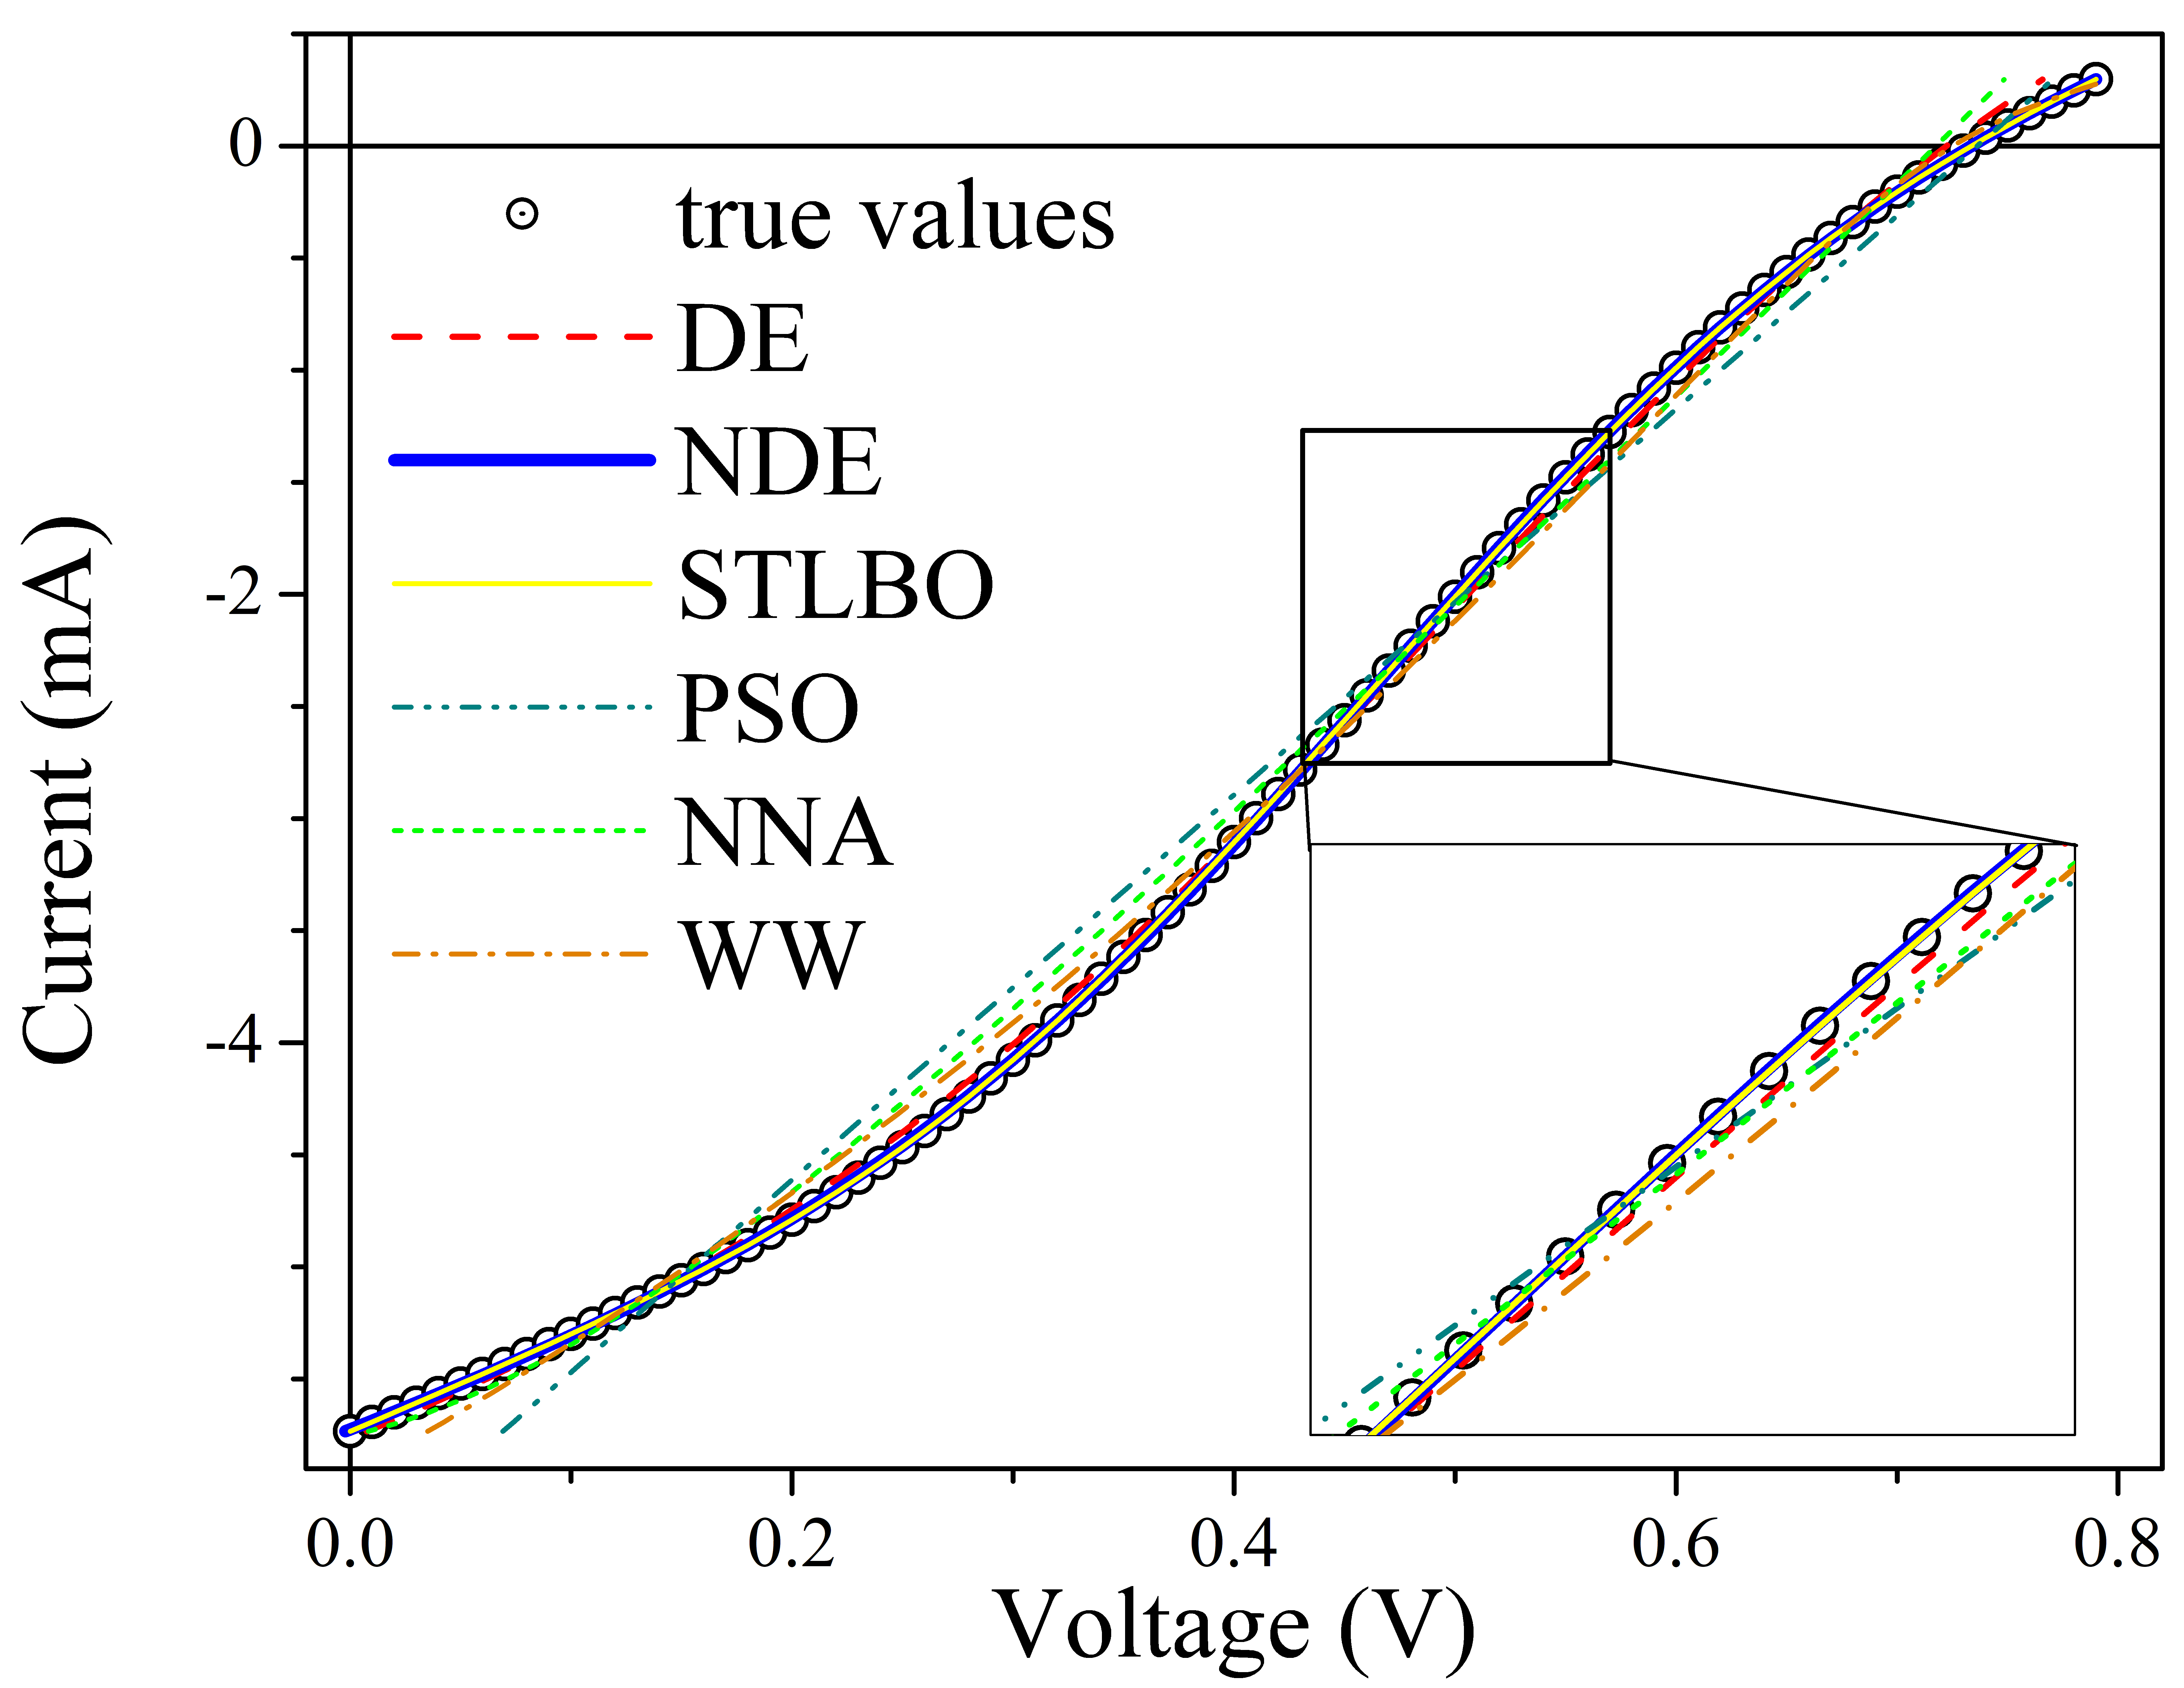
\includegraphics[width=0.5\columnwidth]{Fig2}
	  \caption{The current-voltage characteristic, which used in single-\emph{IV} case (symbols).
        The values from Eq.~(\ref{eqParSingleIV}) were assumed during the simulation.
        The fitting results of various meta---heuristic algorithms are represented by lines.}\label{figSigleIV}
\end{figure}




\subsubsection{IV--set case}\label{SetIV}

Employing various meta--heuristic algorithms to analyze a single \emph{IV} curve
is insufficient for gaining comprehensive insights into the efficacy of these methods in parameter estimation.
Furthermore, the accuracy of parameter determination is closely tied to their exact values.
For example, an increase in the $R_\mathrm{p}$ value can create challenges in accurately estimating resistance
because the shunt will have a reduced impact on the overall shape of the IV curve.
Additionally, the ratio between the parameter values is also crucial.

To test the methods across different parameter values, we generated synthetic data within a temperature range of 260~K to 350~K.
In the simulation process, we considered the temperature dependencies of the parameters.
We based our approach on known physical mechanisms of current flow in NG-SCs and
used the reported temperature dependencies of saturation current, ideality factor, shunt resistance, and series resistance.
However, the main focus was on achieving a diversity of parameter ratios rather
than attempting to precisely replicate real--life PV converters of a specific type.
Furthermore, an S--shaped \emph{IV} curve is observed in various types of solar cells,
and diverse charge transport mechanisms significantly complicate the selection of a single possible temperature dependence for each of the eight model parameters.

Therefore, we assumed that the current conduction mechanism through D1 is close to tunneling.
Hence, $I_{01}$, $R_\mathrm{p1}$, and $(n_1kT)$ remain constant with the selected values
$I_{01}=0.015$~mA, $R_\mathrm{p1}=10^4$~$\Omega$, $n_1kT=7$~eV.
In the case of D2, the thermionic emission current was suggested,
and $I_{02}$ and $n_2$ increased and decreased, respectively, with rising temperature \cite{Sze2012}:
\begin{eqnarray}
%\label{eqIV_W}
I_{02}&=& I_{002}\exp\left(-E_I/kT\right)\,,\\
n_2&=&1+T^*/T\,,
\end{eqnarray}
where
$I_{002}$, $E_I$, and $T^*$ are the constants which are independent of temperature.
The values of $I_{002}=500$~A, $E_I=0.40$~eV, and $T^*=500$~K were used.
For $R_\mathrm{p2}$, an exponential temperature dependence was used,
as it is commonly observed \cite{Kondratenko2019} in NG-SCs for shunt resistance:
\begin{equation}
R_\mathrm{p2}=R_\mathrm{p20}\exp\left(E_R/kT\right)\,
\end{equation}
with
$R_\mathrm{p20}=9$~m$\Omega$,
$E_R=0.32$~eV.
The linear temperature dependencies is expected for both $I_\mathrm{ph}$ \cite{Green2003,Eberle2021} and $R_\mathrm{s}$ \cite{Ibrahim2017,Bradaschia2019}:
\begin{equation}
y=y_{0}[1-\mathrm{TC}_y(T-300)]\,,
\end{equation}
where
$y=I_\mathrm{ph}$ or $R_\mathrm{s}$,
$y_0$ is the parameter value at room temperature,
$\mathrm{TC}_y$ is the temperature coefficient of parameter.
For most types of monocrystalline silicon solar cells, the $\mathrm{TC}_{I_\mathrm{ph}}$ typically ranges from around $-0.0004$~K$^{-1}$ \cite{TuanLe2021}.
However, as the base thickness decreases, the temperature coefficient can increase to $-0.0014$~K$^{-1}$ \cite{Dupre2016}.
For hydrogenated amorphous silicon solar cells, $\mathrm{TC}_{I_\mathrm{ph}}$ is equal to $-10^{-3}$~K$^{-1}$ \cite{Riesen2016}.
For organic solar cells, the temperature coefficient can reach a magnitude of $-0.003$~K$^{-1}$ \cite{Rana2018}.
During the simulation, we assumed $\mathrm{TC}_{I_\mathrm{ph}}=-10^{-3}$~K$^{-1}$.
Furthermore, the values of $I_\mathrm{ph0}=1$~mA,
$\mathrm{TC}_{R_\mathrm{s}}=0.02$~K$^{-1}$,
and $R_\mathrm{s0}=50$~$\Omega$ were used.


The set of \emph{IV} data consisted of 10 curves,
simulated at 10~K intervals from 260~K to 350~K;
in this case,
$n_1$,
$I_{02}$,
$n_2$,
$R_\mathrm{p2}$,
$R_\mathrm{s}$,
and $I_\mathrm{ph}$
varied
from 6.37 to 4.73,
from 9 to 880 $\mu$A,
from 2.92 to 2.43,
from $1.4\cdot10^4$ to 360~$\Omega$,
from 10 to 100~$\Omega$,
and from 0.96 to 1.05~mA, respectively.
The \emph{IV} curves were simulated over a voltage range of 0-1.0~V with a 10~mV step.
The simulation results are depicted in Fig.~\ref{figSetIV} using symbols.

\begin{figure}[]
	\centering
%		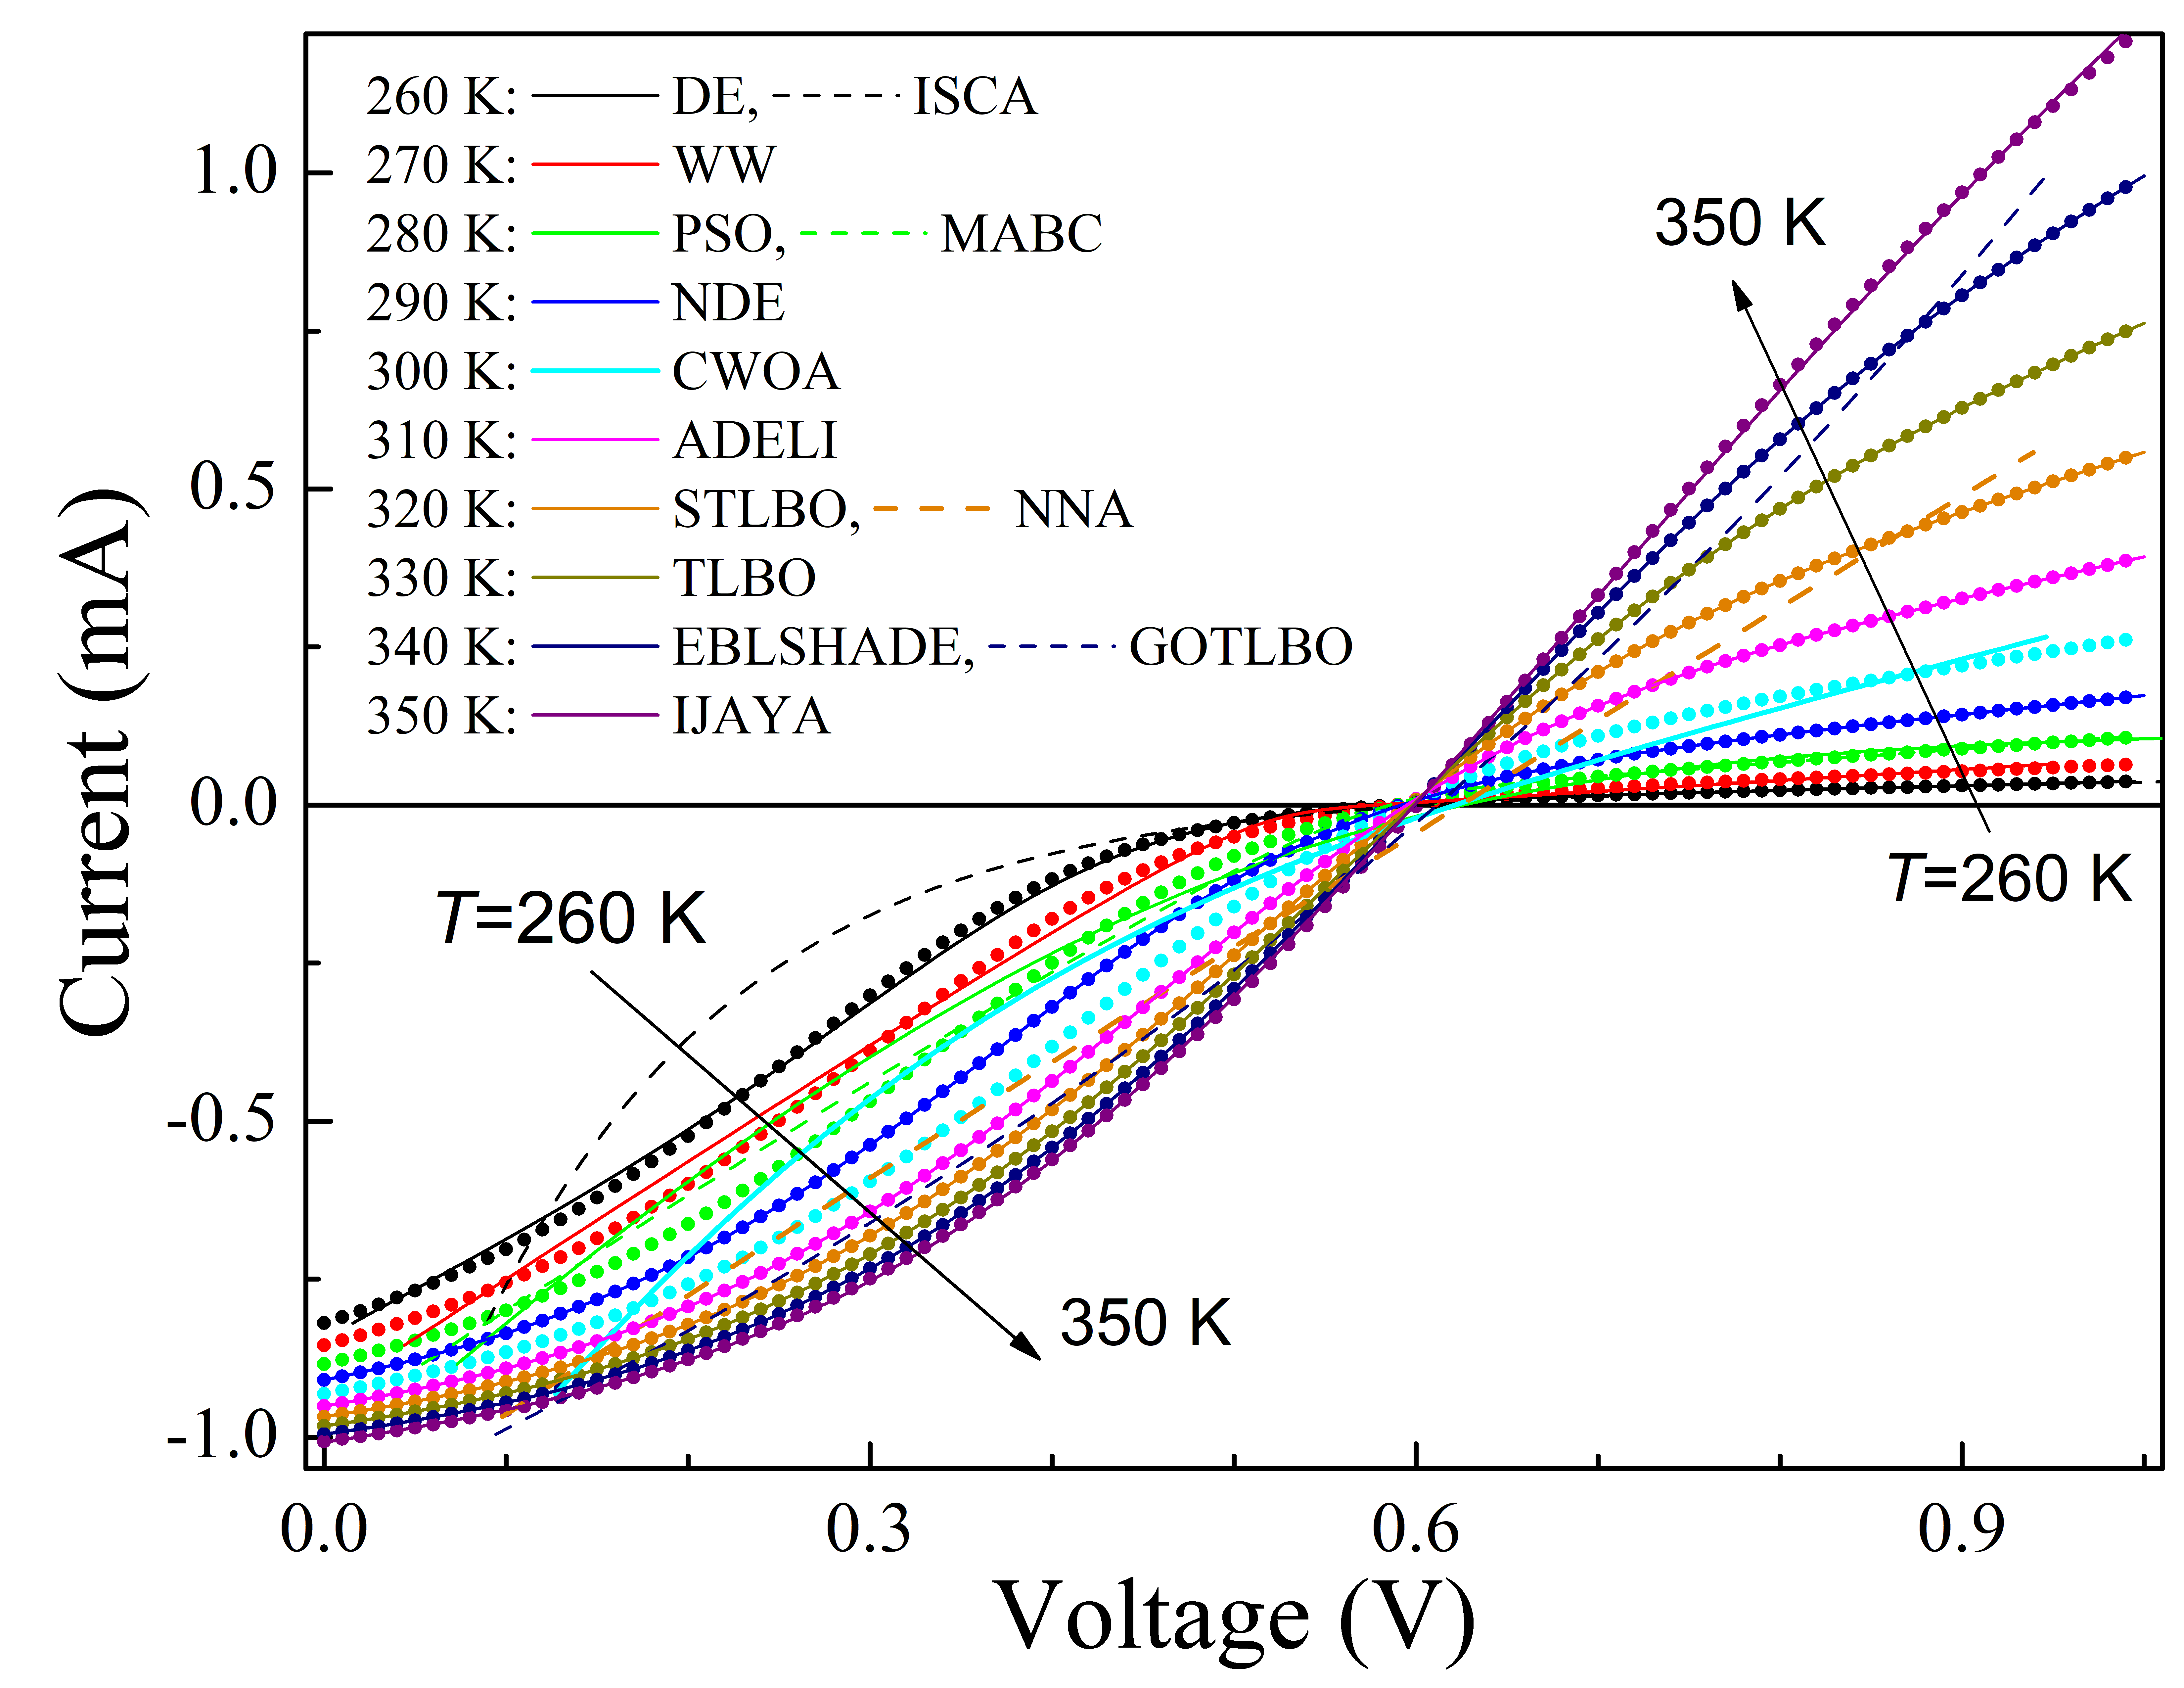
\includegraphics[width=1.0\columnwidth]{IVset}
		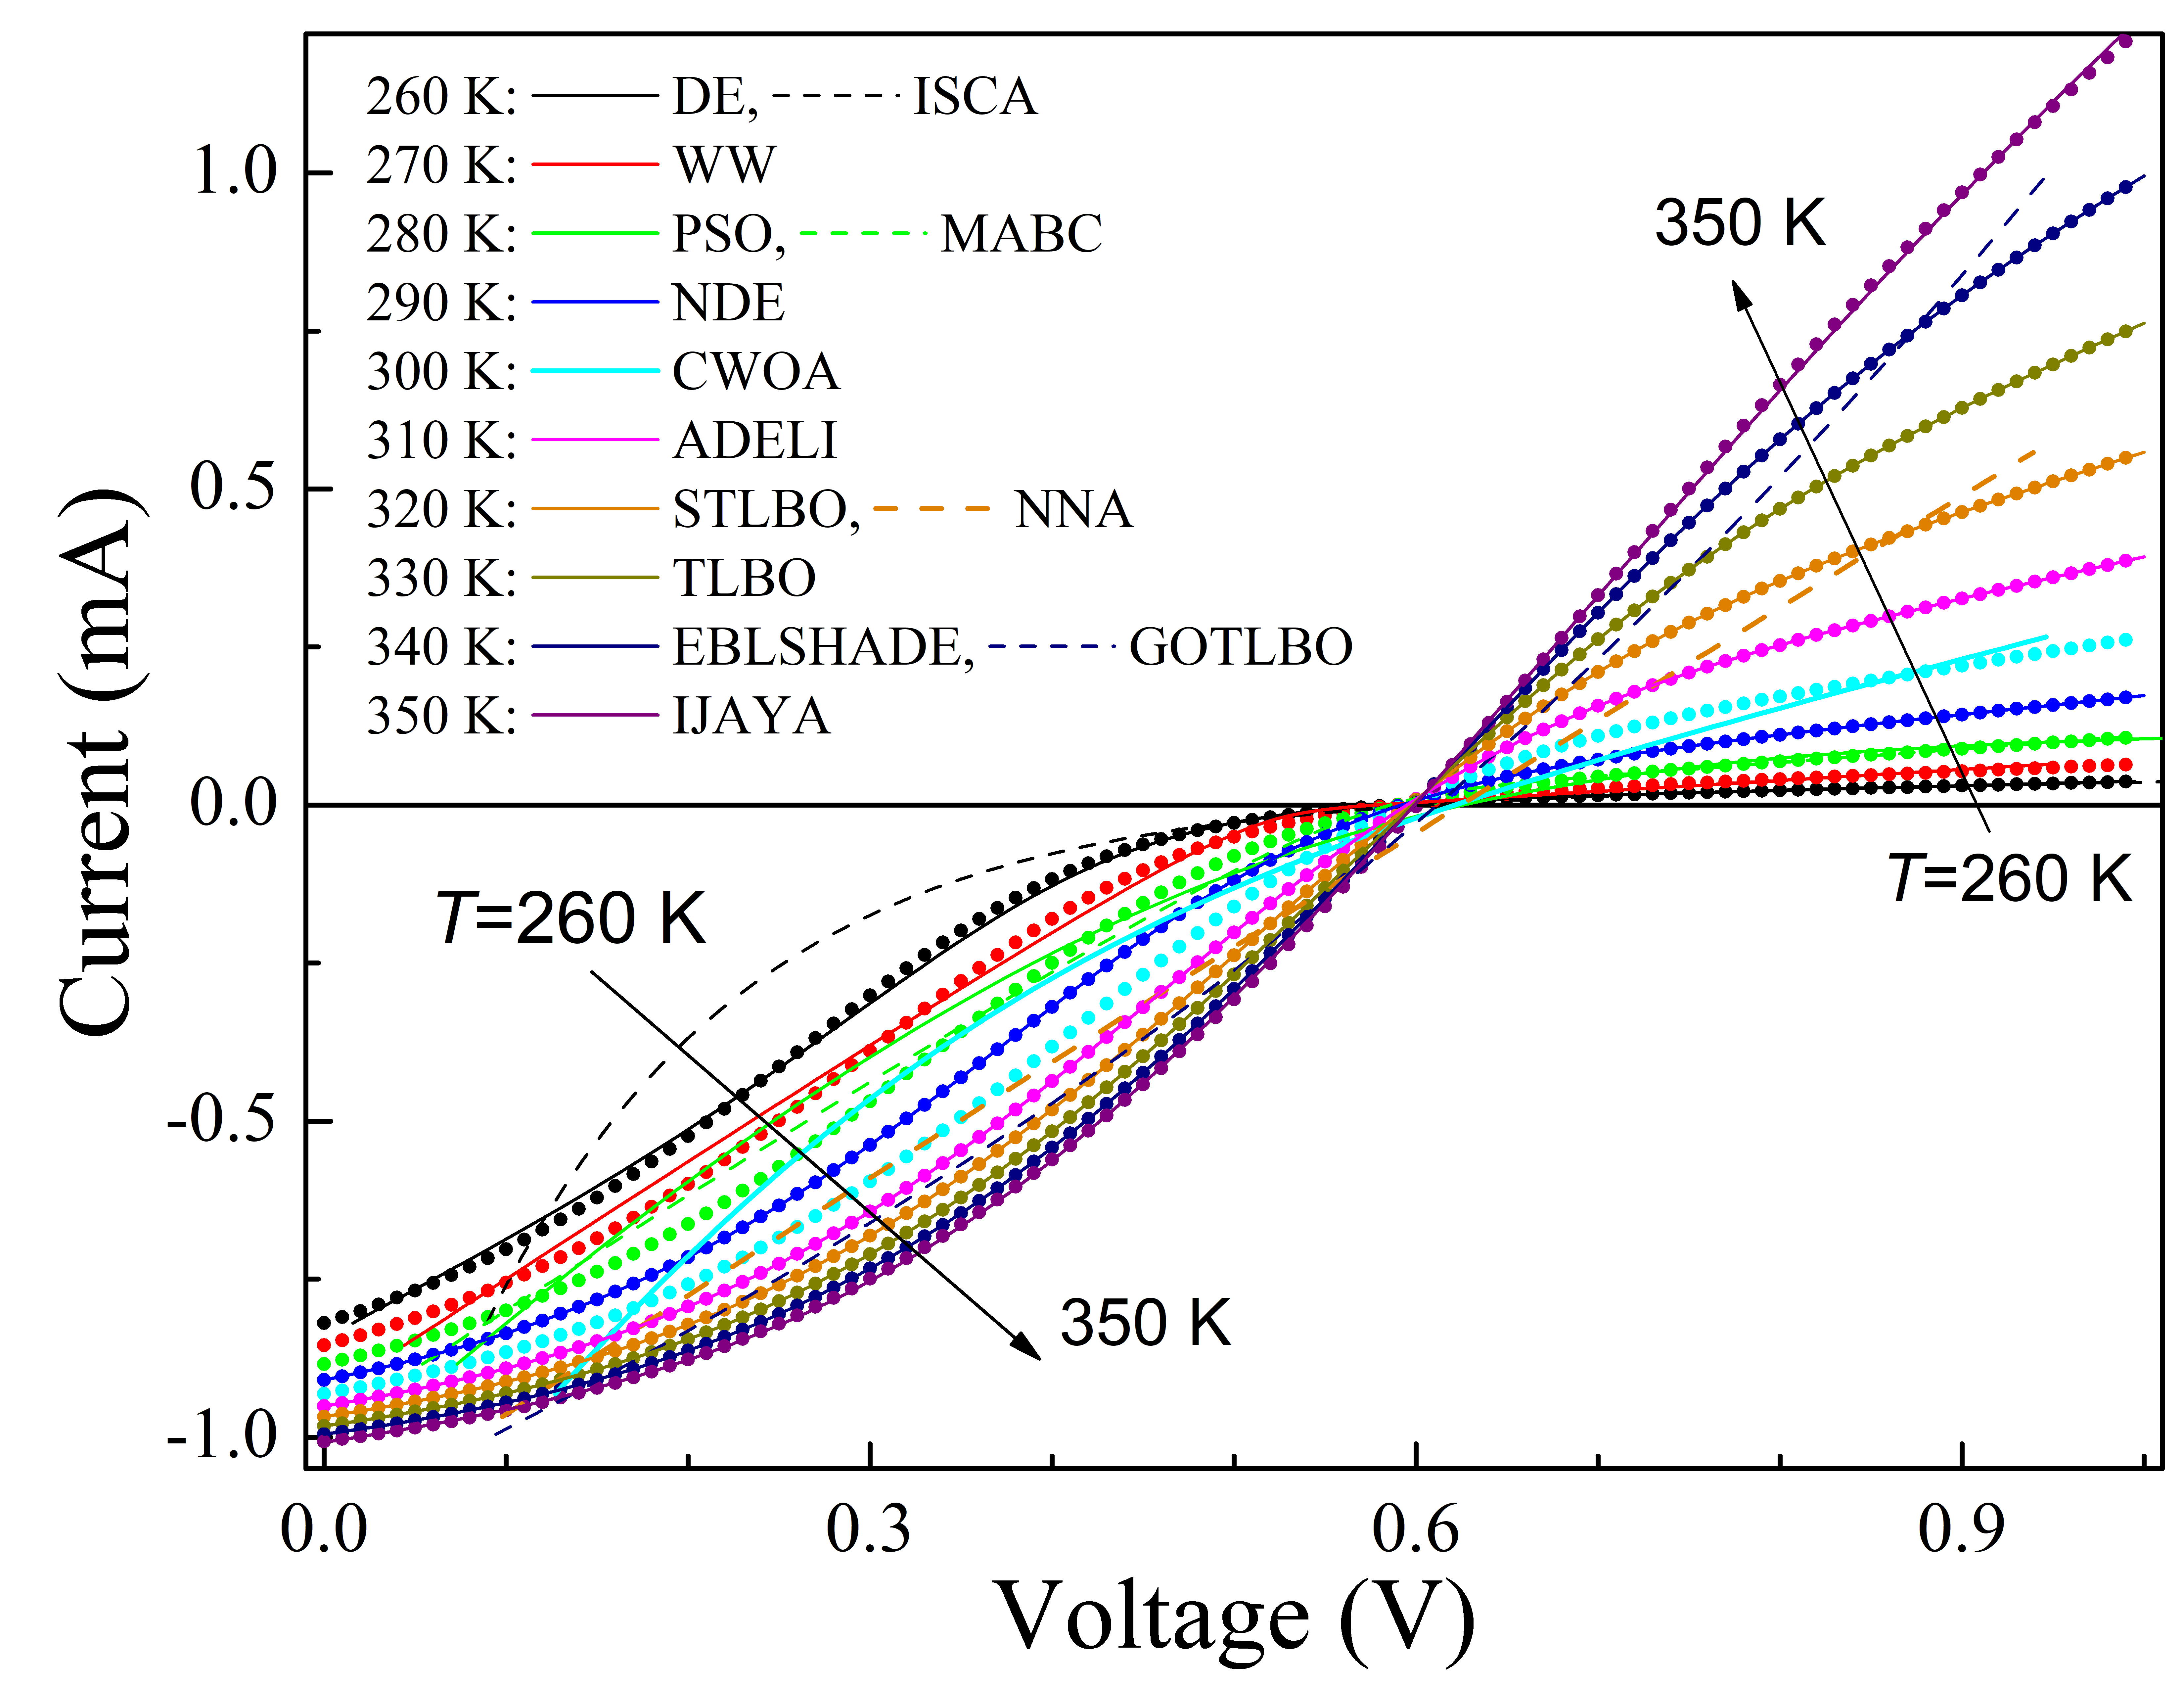
\includegraphics[width=0.5\columnwidth]{Fig3}
	  \caption{The current-voltage characteristics, which used in \emph{IV}-set case (symbols).
        The values from ec.~\ref{SetIV} were assumed during the simulation.
        The fitting results of various meta---heuristic algorithms are represented by lines.}\label{figSetIV}
\end{figure}


\subsection{Meta--heuristic algorithms}\label{MHA}
In the literature, meta--heuristics are frequently categorized based on their sources of inspiration.
This categorization involves blending true simulations with stochastic elements
to mimic various biological behaviors, natural phenomena, and human behavior characteristics.

On this basis, any meta--heuristic algorithm can fall into one of the following main classes \cite{WhiteShark,Gannet,Dandelion}:
evolution-based methods (emulate the principles of evolutionary behavior observed in creatures in nature by relying on the concept of survival of the fittest),
swarm intelligence--based methods (simulate the collective, dynamic, intelligent, and concerted gregarious conduct of collections of flocks or communities found in nature),
bio--based methods (use biological processes unrelated to group behavior),
chemical \& physical--based methods (originate from the physical phenomena or chemical laws that exist in the universe),
human-society--based methods (inspired by human beings, including various activities such as thinking and social behavior),
and math--based methods (borrow the mathematical functions).
Generally, there are hundreds of meta--heuristic optimization methods available.
While we acknowledge that our selection may not be fully comprehensive,
we utilized 14 methods, representing all classes mentioned above,
to tackle the parameter estimation task within the framework of the opposed two-diode model for a solar cell.
Hereafter, we will briefly describe each method and the parameters used during the fitting process.

\emph{Differential evolution} (\textbf{DE}).
DE is one of the classical methods,
and  it is based on the natural selection law, utilizing randomly generated initial populations,
differential mutation, and probability crossover \cite{DEWang}.
We used a penalty function recommended by Ishaque \emph{et al}. \cite{P-DE_Ishaque} during the implementation process.
According to Wang and Ye \cite{DEWang}, this work used the following values:
mutation scaling factor $F=0.8$,
crossover rate $C\!r=0.3$,
and population size $N\!p=8\times D=64$.

\emph{Adaptive differential evolution with the Lagrange interpolation argument} (\textbf{ADELI}).
This improved version of DE incorporates three main elements:
local search using Lagrange interpolation, self-adaptive DE control parameter settings,
and an adaptive mutational strategy \cite{ADELI}.
The first element involves interpolating three potential solutions using a
polynomial function to calculate the local minimum value.
The self-adaptive control parameter settings include randomly altering the
scaling factor and crossover rate values in each iteration.
The adaptive mutational strategy determines the probability of
employing Lagrange interpolation in each generation based on the best fitness function value.
These incorporations aim to enhance exploitation capability and speed up the convergence.
We used parameter values recommended by Huang \emph{et al.} \cite{ADELI} during the implementation process.
Additionally, we set $N\!p$ to 64 for our numerical experiments.

\emph{Differential evolution with neighborhood--based adaptive evolution mechanism} (\textbf{NDE}).
The method employs a mutation strategy that considers neighborhood and individual information, along with an adaptive evolutionary mechanism \cite{NDE}.
$F$ and $C\!r$ values are determined using a weighted adaptive procedure \cite{Tanabe2014}.
The population size is adjusted adaptively using a simple reduction method from $10\times D=80$ to 5.

\emph{Success history based DE with hybridization mutation strategies and population size reduction} (\textbf{EBLSHADE}).
The method represents a hybridization framework between the \emph{pbest} and \emph{ord\_pbest} mutation strategies.
It stores a set of $Cr$ and $F$ values that have shown good performance in the recent past \cite{EBLSHADE}.
A linear $N\!p$ reduction (from $18\times D=144$ to 4) is used as well.

\emph{Particle swarm optimization} (\textbf{PSO}).
It is another classic method based on observations of the social behavior of animals,
such as bird flocking, fish schooling, and swarm theory.
According to Ye et al. \cite{PSO},  the values of learning factors $l_1=l_2=2$,
the final weight and the initial weight $w_{max}=0.9$, $w_{min}=0.4$, and
$N\!p=15\times D=120$ are used in this work.


The \emph{modified artificial bee colony} (\textbf{MABC}) algorithm is inspired
by the intelligent foraging behavior of honey bee swarms \cite{MABC}.
The control parameters include the population size ($N\!p=8\times D=64$)
and the maximum number of generations, ($L_{imit}=36$), after which each non-improved food source is discarded.


\emph{Chaotic Whale Optimization Algorithm} (\textbf{CWOA}).
Initial algorithm (WOA) draws inspiration from the hunting behavior of humpback whales \cite{WOA}.
Whereas CWOA employs chaotic maps to compute and dynamically adjust its internal parameters \cite{CWOA}.
In our study, we utilized the Singer chaotic map and set $N\!p=100$ to identify the SC parameters.

The \emph{neural network algorithm} (\textbf{NNA}) is a meta--heuristic method
inspired by both biological nervous systems and artificial neural networks \cite{NNA}.
In our paper, we used the recommended \cite{NNA} value of $N\!p=50$.

The \emph{teaching learning based optimization} (\textbf{TLBO}) algorithm utilizes the idea of knowledge transfer within a classroom.
Similar to learners acquiring knowledge from a teacher and interacting with their peers,
TLBO incorporates these interactions \cite{TLBO_Patel}.
In this study, a value of $N\!p=100$ is used.

\emph{Generalized oppositional teaching learning based optimization} (\textbf{GOTLBO}).
This method utilizes generalized opposition-based learning to enhance basic TLBO
through the initialization step and generation jumping, improving convergence speed \cite{GOTLBO}.
The values of jumping rate $J\!r=1.0$ and $N\!p=20$ were used.

\emph{Simplified teaching-learning based optimization algorithm} (\textbf{STLBO}).
In STLBO, the teacher phase is redefined and simplified, while the learner phase remains unchanged \cite{STLBO}.
In the redefined teacher phase, the mutation of potential solutions is possible,
with the mutation probability decreasing as the iteration number increases.
During the early stages, a higher mutation probability helps explore a larger solution space
and approach the optimum quickly.
However, in the latter stages of optimization, when the teacher (best solution) is near the global optimum,
a lower mutation probability serves as a fine-tuning mechanism
to enhance local search capability, proving to be an effective strategy.
To enrich the mutation behavior, a chaotic sequence is introduced to generate values for the mutation parameters.
A chaotic sequence is a deterministic, random-like process found in nonlinear dynamic systems,
which is non-periodic, non-converging, and bounded \cite{May1976}.
Additionally, the elite strategy replaces the worst solutions in the current population with new solutions based on objective function values.
The logistic chaotic map and $N\!p=20$ were used.



\emph{Water wave optimization} (\textbf{WW}) takes inspiration from shallow water wave models
and incorporates  ideas from wave propagation, refraction, and breaking \cite{WW}.
WW is easy to implement with a small-size population, and there are four control parameters:
the maximum wave height $h_{max}$,
the wavelength reduction coefficient $\alpha$,
the breaking coefficient $\beta$,
and the maximum number $k_{max}$ of breaking directions.
According to Zheng \cite{WW}, we used
the values $h_{max}=6$, $\alpha=1.026$,  $N\!p=10$,
$k_{max}=\min(12,D/2)=4$, and $\beta$ linearly decreased from 0.25 to 0.001.

\emph{Improved JAYA} (\textbf{IJAYA}).
Jaya algorithm is based on the concept
that the solution obtained for a given problem should move toward the best solution and should
avoid the worst solution and does not require any algorithm-specific parameter \cite{JAYA}.
In IJAYA \cite{IJAYA}, a self-adaptive weight mechanism is introduced to balance
the approach towards the optimal solution while simultaneously avoiding the suboptimal solutions.
An experience-based learning strategy is utilized to preserve population diversity and enhance exploration capabilities.
Additionally, a chaotic elite learning method is proposed to refine the quality of the best solution in each generation.
The logistic chaotic map and $N\!p=4\times D=32$ were used.

\emph{Improved sine cosine algorithm} (\textbf{ISCA}).
SCA is based on simulating the behaviors of sine and cosine mathematical functions \cite{SCA}.
ISCA implementation included a modified position-updating equation based on inertia weight
($w_{start}=1$, $w_{end}=1$),
a nonlinear conversion parameter strategy based on the Gaussian function
($a_{start}=2$, $a_{end}=0$) \cite{ISCA2},
the creation of the opposite population to jump out from the local optima with $J\!r=0.1$ \cite{ISCA3},
a greedy selection, and $N\!p=30$.

The majority of the algorithms used show excellent performance
in estimating the SC parameter within conventional models such as SDM or DDM
\cite{CWOA,DEWang,GOTLBO,IJAYA,MABC,PSO,STLBO,TLBO_Patel,LSHADE,IWOA}.


In meta--heuristic optimization methods, the quality of the extracted parameters is evaluated using the fitness function at
every iteration.
In our investigation, we considered absolute error and square error fitness functions:
\begin{gather}
\label{eqFae}
F_\mathrm{AE}(Y)= \sum_{k=1}^p \left|V^\mathrm{tr}(I_k)-V^\mathrm{cal}(I_k,Y)\right|\,,\\
\label{eqFse}
F_\mathrm{SE}(Y)= \sum_{k=1}^p \left[V^\mathrm{tr}(I_k)-V^\mathrm{cal}(I_k,Y)\right]^2\,,
\end{gather}
where
$V^\mathrm{tr}(I_k)$ is the simulated value of voltage at current $I_k$,
$V^\mathrm{cal}(I_k,Y)$ represents the voltage,
which is calculated using a set of parameters
(i.e. $Y = \{I_{01},n_1,R_\mathrm{p1},I_{02},n_2,R_\mathrm{p2},R_\mathrm{s},I_\mathrm{ph}\}$)
estimated with the help of an algorithm and Eqs.~(\ref{eqIV_g})--(\ref{eqx2});
and $p$ is the total number of voltage steps in the \emph{IV} characteristic.

We executed each tested algorithm for $N_\mathrm{runs}=51$ independent runs on every  simulated \emph{IV} curve
to generate the statistical results.
The search ranges were set as follows:

\noindent
$I_{01}(\mathrm{mA})\in[10^{-13},1]$,
$n_1\in[0.5,50]$,
$R_\mathrm{p1}(\Omega)\in[10,10^6]$,
$I_{02}(\mathrm{mA})\in[10^{-7},10]$,
$n_2\in[0.5,50]$,
$R_\mathrm{p2}(\Omega)\in[10,5\cdot10^4]$,
$R_\mathrm{s}(\Omega)\in[0.1,1000]$,
$I_\mathrm{ph}(\mathrm{mA})\in[10^{-3},100]$.





\subsection{Evaluation metrics}\label{EvalCr}

To better illustrate the performance differences between the algorithms being compared,
we considered several evaluation metrics.
These metrics can be described as follows:
\begin{enumerate}[1.]
\item
Mean value (MEAN), median value (MEDIAN), standard deviance (STD), and interquartile range (IQR)
for each two--diode model parameter $y$
($y$ is one of $\left\{I_{01}\right.$, $n_1$, $R_\mathrm{p1}$, $I_{02}$, $n_2$, $R_\mathrm{p2}$, $R_\mathrm{s}$, $\left.I_\mathrm{ph}\right\}$).
MEAN and MEDIAN are often used to measure the solution quality.
The closer the obtained MEAN and MEDIAN values are to the actual parameter values,
the closer the obtained solution is to the optimal solution.
To quantify, we used the  absolute percentage error (APE):
\begin{equation}
\label{eqAPE}
\mathrm{APE}\,(y)= \left| \frac{y-y^\mathrm{tr}}{y^\mathrm{tr}}\right|\,,
\end{equation}
where
$y^\mathrm{tr}$ is the parameter value used during the \emph{IV} curve simulation.
APE was calculated for $y_i$, obtained by one--run algorithm application ($\mathrm{APE}_i$),
MEAN ($\mathrm{APE}_\mathrm{MEAN}$), and MEDIAN ($\mathrm{APE}_\mathrm{MEDIAN}$).
Reducing STD and IQR result in a more stable algorithm performance.

\item
Another criterion for evaluating and comparing algorithm performance is their execution time.
We used average run time $t_\mathrm{run}$ in seconds for an
individual optimizer on one IV curve.

\item
The root mean square percentage error (RMSPE) is a statistical measure that indicates
how well the fitted curve matches the actual (simulated) \emph{IV} curve.
\begin{equation}
\label{eqRMSPE}
\mathrm{RMSPE}= \sqrt{\frac{1}{p} \sum_{k=1}^p \left[\frac{V^\mathrm{tr}(I_k)-V^\mathrm{cal}(I_k,Y)}{V^\mathrm{tr}(I_k)} \right]^2}\,.
\end{equation}

\item
Wilcoxon signed-rank test is a nonparametric statistical test used for pairwise comparisons of algorithms.
This test assigns a rank to all the scores considered as one group and then sums the ranks of each group.

\item
Friedman, Friedman Aligned, and Quade tests are used for comparing the performance differences
among optimization algorithms
(multiple comparisons with a control method).
Therefore, the average rankings of the algorithms according to the
tests are reported.
Besides, the post--hoc  Finner, Holm, Hochberg, and Holland procedures
are used to establish proper comparisons between each algorithm and a set of other algorithms.

\item
Multiple Comparisons Test (Friedman) with Shaffer’s static, Nemenyi, and Holm procedures
are employed to compute all possible pairwise comparisons between groups ($N\times N$)
and identify the differences.

\end{enumerate}


Wilcoxon test is used to assess whether there are statistically significant differences between pairs of algorithms.
Meanwhile, the Friedman, Friedman Aligned, and Quade tests are employed when it's necessary to compare three or more related groups of results (algorithms).
Friedman test evaluates whether there are statistically significant differences between the medians of the ranks of these algorithms.
Friedman Aligned Ranks test addresses the issue of rank correlation in the original Friedman test, providing more precise results.
Finally, the Quade test helps account for the effects of observed factors, such as random variations,
to more accurately determine the statistical differences between groups.

The main drawback of the Friedman, Friedman Aligned, and Quade tests is that
they can only detect significant differences over the whole set of multiple comparisons,
making it difficult to establish proper comparisons between specific algorithms \cite{Derrac2011}.
To address these issues, it is necessary to employ post-hoc procedures.
Post-hoc methods are applied after the initial analysis and allow for controlling the overall error rate
when comparing multiple algorithms, thereby reducing the likelihood of randomly identifying statistically significant differences.

$1\times N$ designs help determine if there are statistically significant differences between one algorithm
(the control algorithm) and each of the other algorithms.
Multidimensional comparisons $N\times N$ designs involve analyzing statistical differences between all possible pairs of algorithms.
Typically, different post-hoc procedures are used for $1\times N$ and $N\times N$ comparisons.
Description of all the used post-hoc procedures can be found in Derrac \emph{et al.} \cite{Derrac2011}.

All mentioned methods are standard for comparing metaheuristic algorithms \cite{Derrac2011}.
Their comprehensive application enables making the most well-founded conclusions.




\section{Numerical results and discussion}\label{Result}



\subsection{Comparison of algorithm convergence}
In meta--heuristic algorithms, various termination conditions can be defined.
For instance, a termination condition can be a specific number of iterations $N_\mathrm{it}$,
constraints on the number of fitness function evaluations $N_\mathrm{FE}$,
a specific rate of precision,
a specific time,
no sign of change in solutions after a specific number of iterations,
or a combination of these cases \cite{IntelligentChaoticClonal}.
In this study, the main focus was on accurately estimating parameters.
Therefore, to ensure that both exploration and exploitation processes
could be fully realized by each algorithm with an equal opportunity,
the termination criterion used was the absence of changes in the solution.
Based on this condition, the required number of iterations $N_\mathrm{it}$ was determined,
and the corresponding calculation time was measured $t_\mathrm{run}$.
Fig.~S1 in the supplementary material shows the convergence curve for the algorithms used.
In addition, the $N_\mathrm{FE}$ were evaluated.

All the applied algorithms have been coded and implemented in Embarcadero\textregistered Delphi $10.3$ programming software.
The run time was estimated by using WinAPI-functions \emph{QueryPerformanceCounter()} and \emph{QueryPerformanceFrequency()}.
The experiments were performed on Windows 10 Pro 64-bit,
2.9 GHz AMD Ryzen 7 4800H CPU, and 8~GB RAM.


\begin{table}[<options>]
\caption{The convergence parameters for metaheuristic algorithms in a single--\emph{IV} case}\label{tblRun}
\begin{tabular*}{\tblwidth}{@{}LCCC@{}}
\toprule
Algorithm  &  $N_\mathrm{it}$ & $N_\mathrm{FE}$ & $t_\mathrm{run}$ (s)\\ % Table header row
\midrule
DE & 8000& 1024000& $42\pm1$\\
EBLSHADE & 3000& 444600& $22\pm1$\\
ADELI & 12000& 1800000& $93\pm2$\\
NDE & 5000& 430000&$20.2\pm0.3$ \\
MABC & 8000& 1024000&$48\pm11$ \\
TLBO & 5000& 1000000&$56.1\pm0.3$ \\
GOTLBO & 6000& 360000&$15\pm1$ \\
STLBO & 13000& 273000&$13.8\pm0.3$ \\
PSO & 4000& 480000&$19\pm3$ \\
IJAYA & 30000& 960000&$37\pm1$ \\
ISCA & 5000& 150000&$6.5\pm0.1$ \\
NNA & 5000& 250000&$10.6\pm0.5$ \\
CWOA & 3000& 300000&$16.6\pm0.5$ \\
WW & 3000& 35000&$1.4\pm0.1$ \\
\bottomrule
\end{tabular*}
\end{table}

The obtained results are listed in Table~\ref{tblRun}.
As can be seen from the table, the number of iterations required for an algorithm does not always correlate directly
with the number of fitness function evaluations or computation time needed to converge.
The reason for this is the unique mathematical operations required by each algorithm.
The run time of the algorithms varies considerably, with a range of 1.5 seconds to 93 seconds.
Notably, WW, ISCA, NNA, and STLBO converge the fastest, while ADELI, TLBO, and MABC require the most time.

\subsection{Fitness function selection}

To choose the more suitable fitness function, we evaluated each algorithm using the IV curve generated from the parameters
provided in Eq.~(\ref{eqParSingleIV}) with both $F_\mathrm{AE}$ and $F_\mathrm{SE}$ functions (see Eqs.~(\ref{eqFae}) and (\ref{eqFse})).
The results obtained from each of the functions were then compared with each other using pairwise comparisons.
The absolute percentage error values obtained for one-run algorithm application ($\mathrm{APE}_i$) were used.
Table~\ref{tblFF} gives the statistical results produced by Wilcoxon sign-rank test with a significant level $\alpha = 0.05$.
The symbol ``SE'' in a cell indicates that the estimation of the parameter (specified in the column title)
by the algorithm (defined in the first column) with $F_\mathrm{SE}$ outperforms the result obtained by this algorithm with $F_\mathrm{AE}$.
A cell with ``AE'' indicates better results for function $F_\mathrm{AE}$.
In the case of the symbol ``='', there is no significant difference between function $F_\mathrm{SE}$ and function $F_\mathrm{AE}$ application.



\begin{table}[<options>]
\caption{Wilcoxon signed rank test results (level of significance $\alpha = 0.05$) for comparing fitness functions.}\label{tblFF}
\begin{tabular*}{\tblwidth}{@{}LCCCCCCCCC@{}}
\toprule
\multirow{2}{*}{Algorithm}& \multicolumn{9}{C}{Parameter} \\
  & $I_{01}$& $n_1$ & $R_\mathrm{p1}$ &$I_{02}$& $n_2$& $R_\mathrm{p2}$&$R_\mathrm{s}$&$I_\mathrm{ph}$&RMSPE\\ % Table header row
\midrule
%\rowcolor{ligthYellow}
DE &\cellcolor{ligthRed}SE &\cellcolor{ligthRed}SE &\cellcolor{ligthYellow}= & \cellcolor{ligthYellow}= &\cellcolor{ligthRed}SE &\cellcolor{ligthRed}SE &\cellcolor{ligthYellow}=  &\cellcolor{ligthYellow}=  &\cellcolor{ligthYellow}= \\
EBLSHADE &\cellcolor{ligthRed}SE &\cellcolor{ligthYellow}=  &\cellcolor{ligthYellow}=  &\cellcolor{ligthYellow}=  &\cellcolor{ligthYellow}=  &\cellcolor{ligthYellow}=  &\cellcolor{ligthYellow}=  &\cellcolor{ligthYellow}=  &\cellcolor{ligthBlue} AE \\
ADELI &\cellcolor{ligthRed}SE &\cellcolor{ligthYellow}=  & \cellcolor{ligthYellow}= & \cellcolor{ligthYellow}= & \cellcolor{ligthYellow}= & \cellcolor{ligthYellow}= &\cellcolor{ligthYellow}=  &\cellcolor{ligthYellow}=  & \cellcolor{ligthBlue} AE\\
NDE &\cellcolor{ligthYellow}=  &\cellcolor{ligthYellow}=  &\cellcolor{ligthYellow}=  &\cellcolor{ligthYellow}=  &\cellcolor{ligthYellow}=  &\cellcolor{ligthYellow}=  & \cellcolor{ligthYellow}= &\cellcolor{ligthRed}SE &\cellcolor{ligthRed}SE \\
MABC & \cellcolor{ligthYellow}= &\cellcolor{ligthRed}SE &\cellcolor{ligthYellow}=  & \cellcolor{ligthYellow}= &\cellcolor{ligthYellow}=  &\cellcolor{ligthYellow}=  &\cellcolor{ligthYellow}=  &\cellcolor{ligthYellow}=  &\cellcolor{ligthRed}SE \\
TLBO &\cellcolor{ligthRed}SE &\cellcolor{ligthRed}SE &\cellcolor{ligthRed}SE & \cellcolor{ligthRed}SE& \cellcolor{ligthRed}SE&\cellcolor{ligthRed}SE &\cellcolor{ligthRed}SE &\cellcolor{ligthRed}SE &\cellcolor{ligthRed}SE \\
GOTLBO &\cellcolor{ligthYellow}=  &\cellcolor{ligthYellow}=  &\cellcolor{ligthYellow}=  &\cellcolor{ligthYellow}=  &\cellcolor{ligthYellow}=  &\cellcolor{ligthRed}SE &\cellcolor{ligthYellow}=  &\cellcolor{ligthYellow}=  &\cellcolor{ligthYellow}=  \\
STLBO &\cellcolor{ligthRed}SE &\cellcolor{ligthYellow}=  &\cellcolor{ligthYellow}=  &\cellcolor{ligthYellow}=  &\cellcolor{ligthYellow}=  &\cellcolor{ligthYellow}=  &\cellcolor{ligthYellow}=  &\cellcolor{ligthYellow}=  &\cellcolor{ligthBlue} AE \\
PSO &\cellcolor{ligthYellow}=  &\cellcolor{ligthYellow}=  &\cellcolor{ligthYellow}=  &\cellcolor{ligthYellow}=  &\cellcolor{ligthYellow}=  &\cellcolor{ligthYellow}=  &\cellcolor{ligthBlue} AE &\cellcolor{ligthYellow}=  &\cellcolor{ligthYellow}=  \\
IJAYA &\cellcolor{ligthBlue} AE &\cellcolor{ligthBlue} AE & \cellcolor{ligthYellow}= &\cellcolor{ligthYellow}=  &\cellcolor{ligthRed}SE & \cellcolor{ligthYellow}= & \cellcolor{ligthYellow}= &\cellcolor{ligthYellow}=  &\cellcolor{ligthYellow}=  \\
ISCA &\cellcolor{ligthYellow}=  &\cellcolor{ligthYellow}=  &\cellcolor{ligthYellow}=  &\cellcolor{ligthYellow}=  &\cellcolor{ligthYellow}=  &\cellcolor{ligthYellow}=  &\cellcolor{ligthYellow}=  &\cellcolor{ligthYellow}=  &\cellcolor{ligthYellow}=  \\
NNA &\cellcolor{ligthYellow}=  &\cellcolor{ligthYellow}=  &\cellcolor{ligthYellow}=  &\cellcolor{ligthYellow}=  &\cellcolor{ligthYellow}=  &\cellcolor{ligthYellow}=  &\cellcolor{ligthYellow}=  &\cellcolor{ligthYellow}=  & \cellcolor{ligthRed}SE\\
CWOA &\cellcolor{ligthYellow}=  &\cellcolor{ligthYellow}=  & \cellcolor{ligthRed}SE&\cellcolor{ligthYellow}=  & \cellcolor{ligthBlue} AE&\cellcolor{ligthYellow}=  &\cellcolor{ligthYellow}=  &\cellcolor{ligthYellow}=  &\cellcolor{ligthRed}SE \\
WW &\cellcolor{ligthYellow}=  &\cellcolor{ligthYellow}=  & \cellcolor{ligthRed}SE& \cellcolor{ligthYellow}= &\cellcolor{ligthBlue} AE & \cellcolor{ligthYellow}= &\cellcolor{ligthYellow}=  &\cellcolor{ligthYellow}=  & \cellcolor{ligthRed}SE\\
\bottomrule
\end{tabular*}
\end{table}

As evidenced in the provided data, utilizing the square error fitness function more frequently yields better outcomes than $F_\mathrm{AE}$.
In some rare cases, the absolute error fitness function can improve the alignment
between the fitted and actual curves and
enhance the accuracy of parameter estimations by PSO, IJAVA, CWOA, and WW algorithms.
However, RMSPE is not the most crucial factor in determining model parameters, and the mentioned methods,
as will be shown later, do not provide the highest accuracy.
As such, the results presented in the following sections exclusively apply the $F_\mathrm{SE}$ function.
Therefore, it is recommended that researchers consider
the squared error fitness function as a more effective and reliable option for the task of opposed two-diode model parameter estimation.


\subsection{Comparison of algorithm performance}

\subsubsection{Parameter extraction in single--IV case}
In this subsection, we present and analyze the statistical results of
applying different meta-heuristic algorithms to an \emph{IV} curve simulated with the values from Eq.~(\ref{eqParSingleIV}).
Several typical fitting results are shown in Fig.~\ref{figSigleIV}.
A more comprehensive version, including the fitting results obtained using each algorithm,
is provided in the supplementary materials (figure S2).
It can be seen that the closest match between the approximation curves and the \emph{IV} curve points is
observed for EBLSHADE, ADELI, NDE, IJAYA, TLBO, and STLBO.
On the contrary, the fitting curves of PSO and GOTLBO had the least replication of the original data.

Fig.~\ref{figBoxSingleIV} shows the results of SC parameters estimation by algorithms to be compared.
Additionally, the figure presents the RMSPE data,
which confirms the conclusions of the visual comparison between the fitting lines and the points of the \emph{IV} curve.
The results for MEAN, MEDIAN, STD, and IQR are presented in table~S1 of the supplementary material.


\begin{figure*}[]
	\centering
		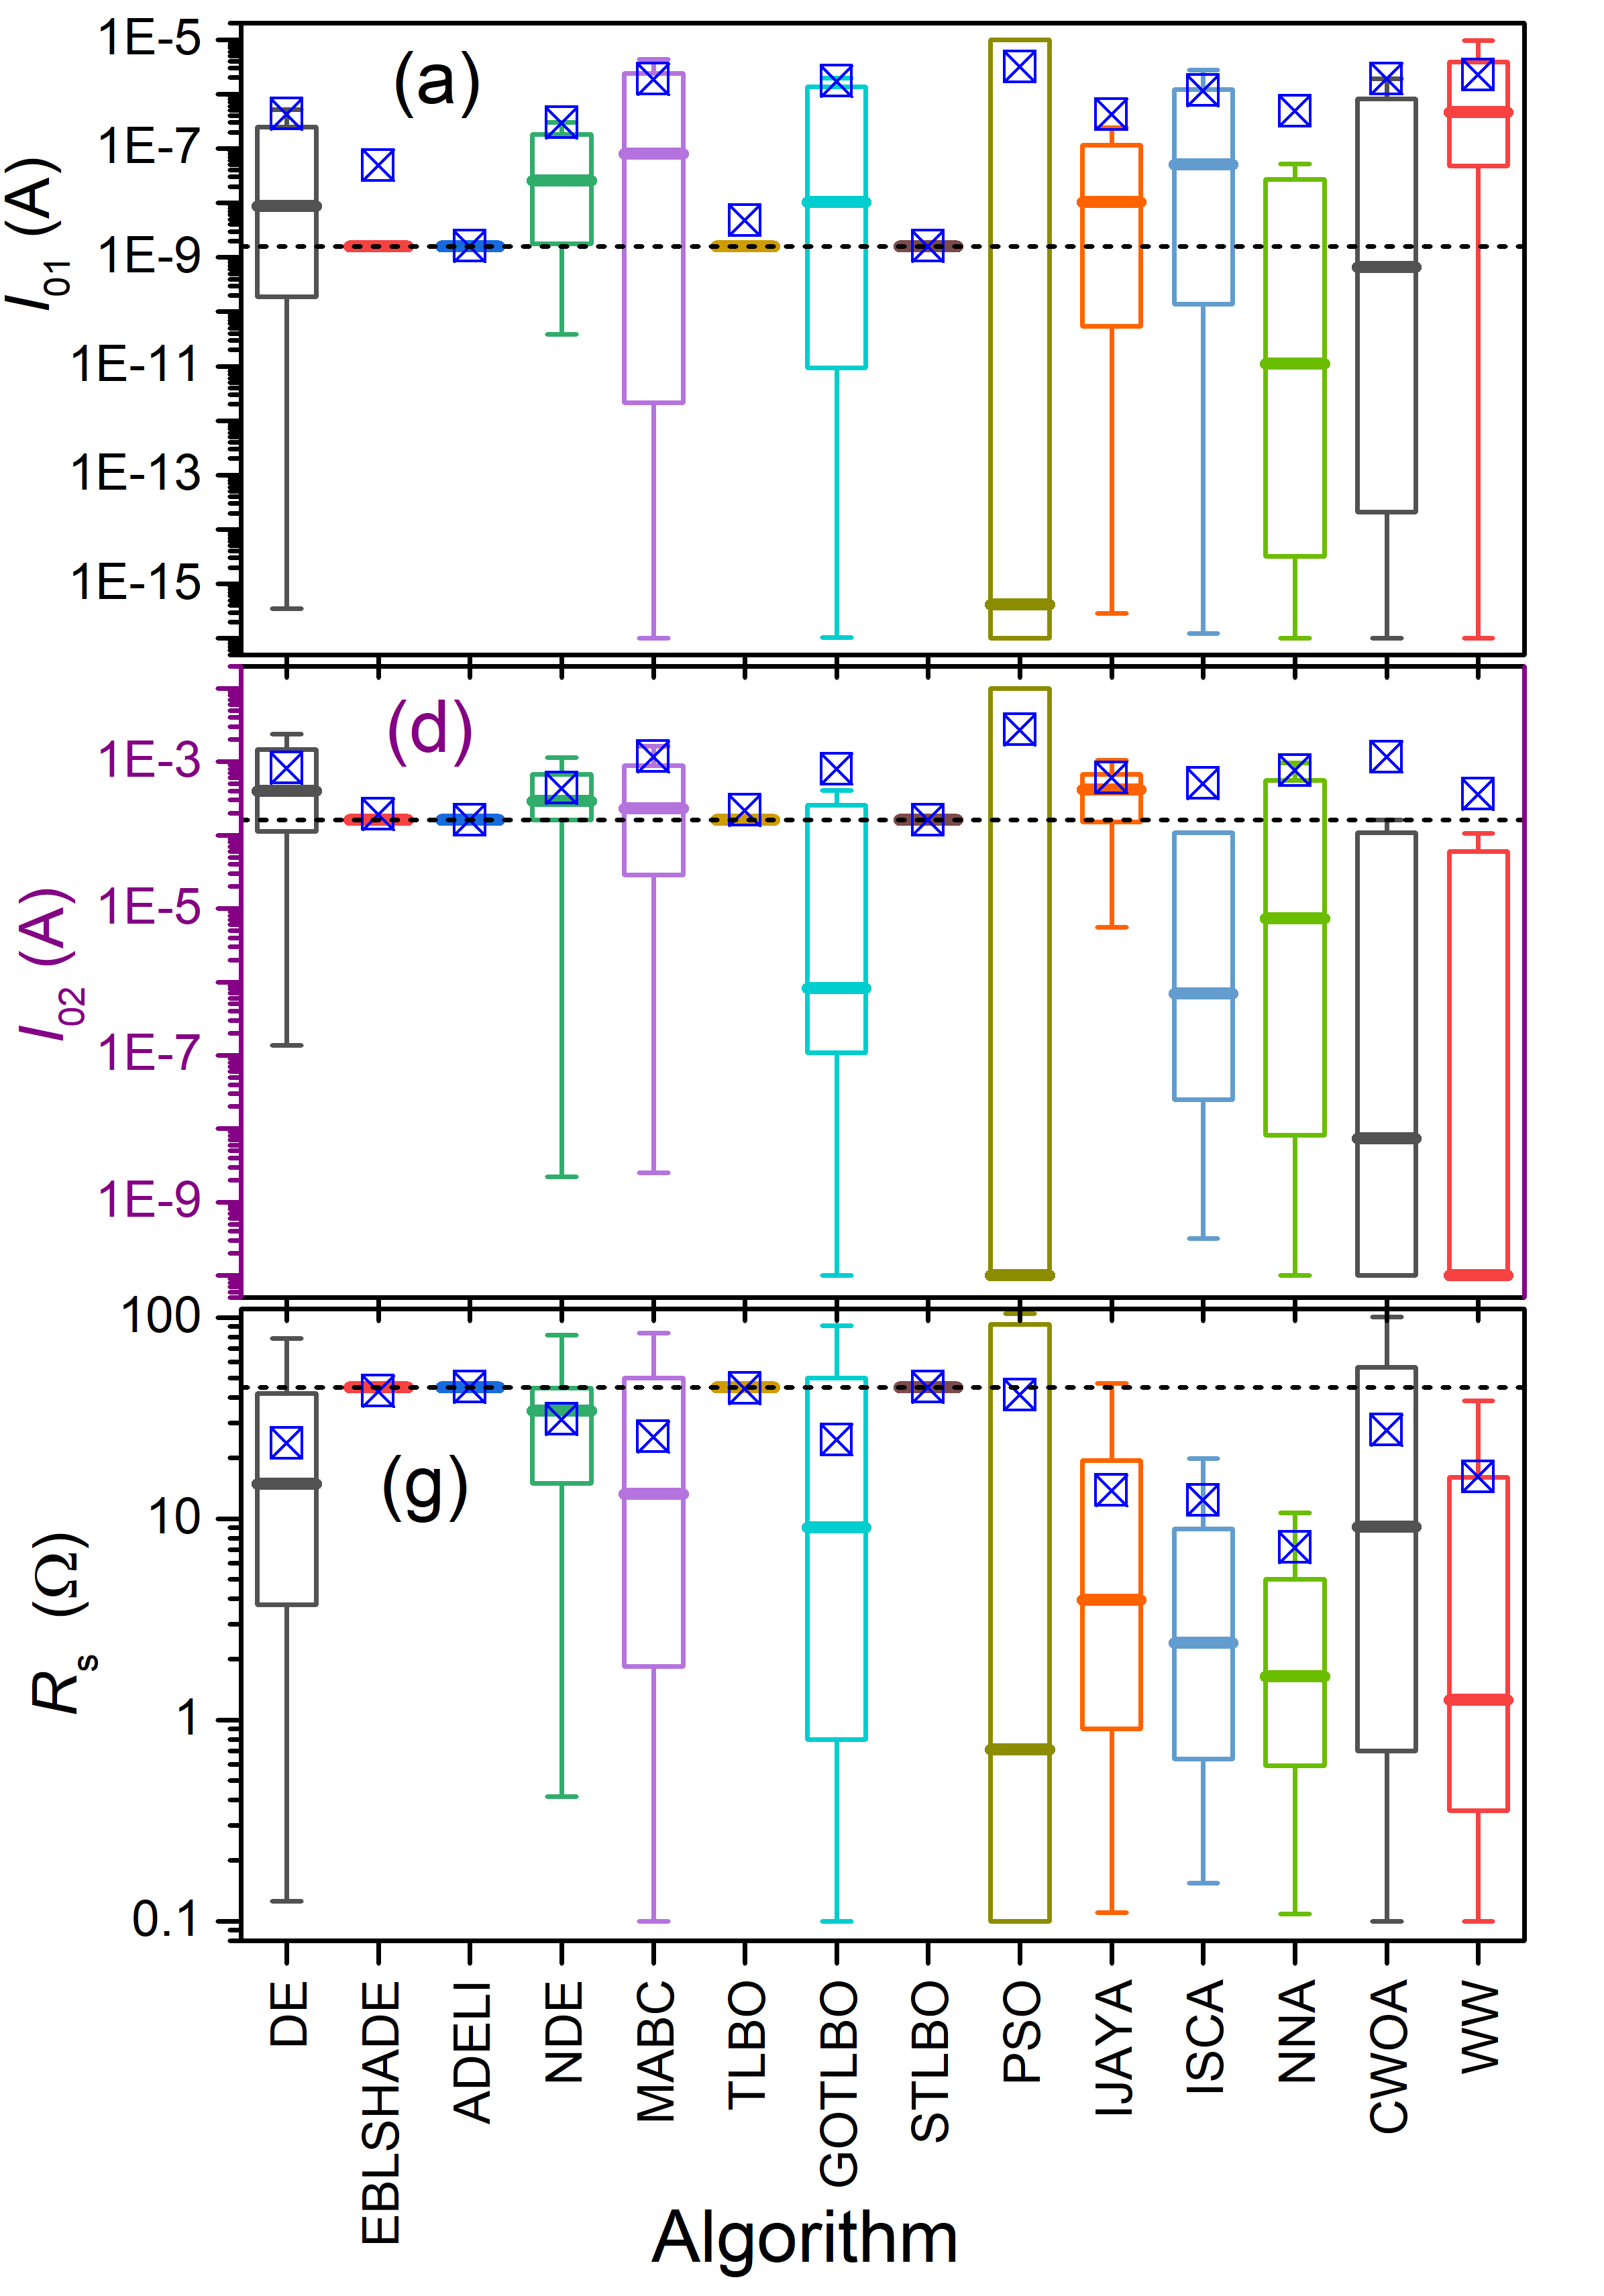
\includegraphics[width=.32\textwidth]{Fig4a}
        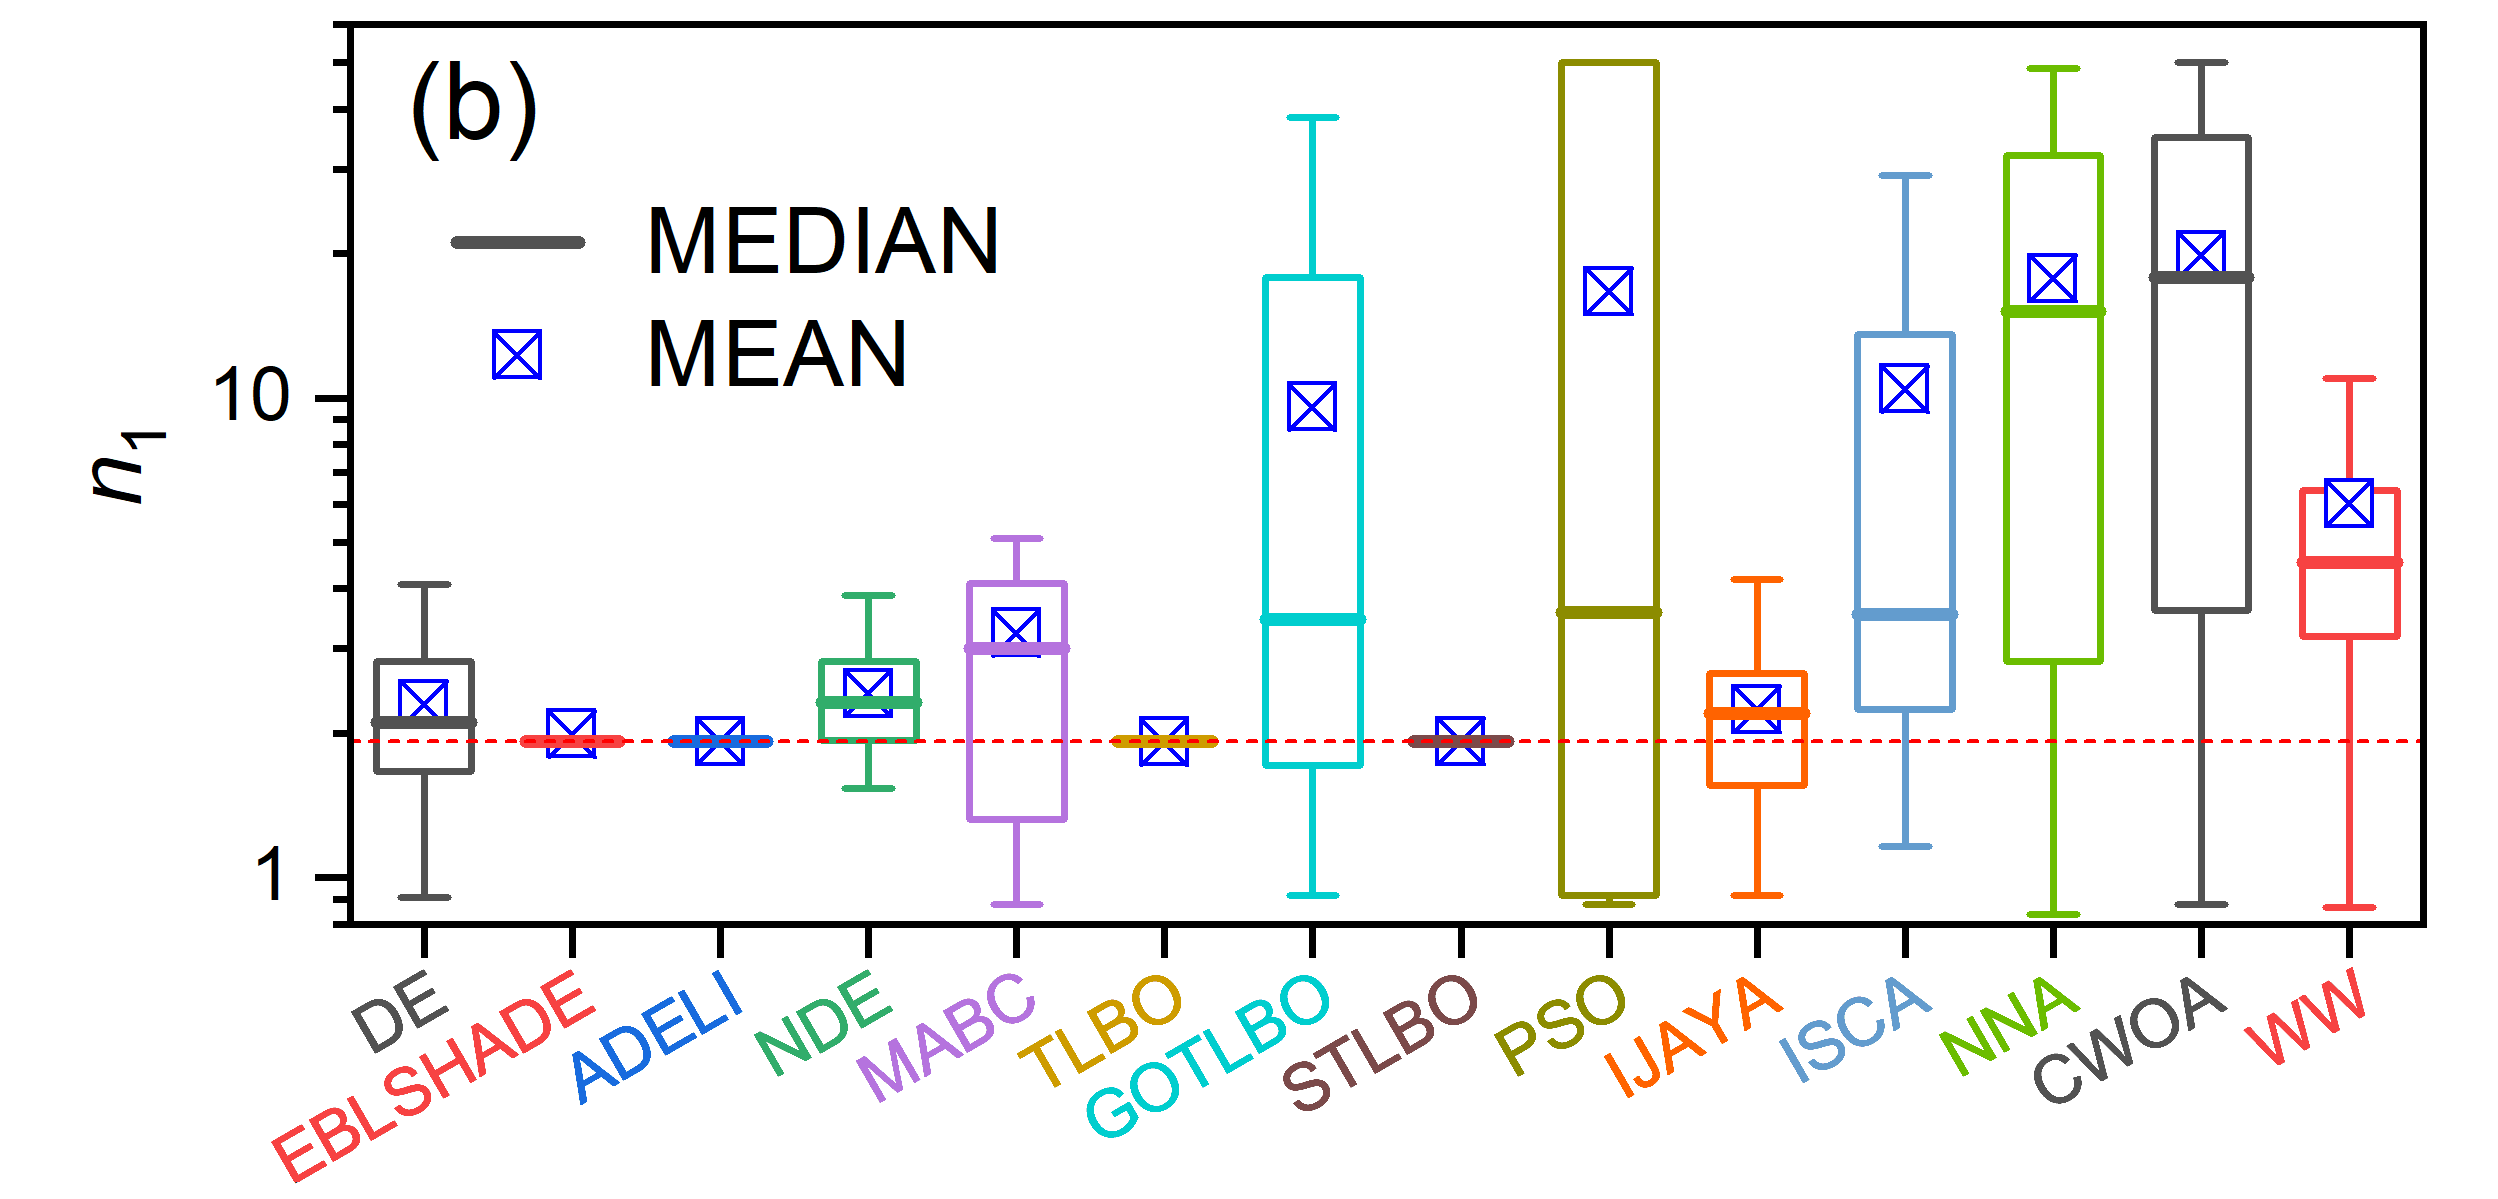
\includegraphics[width=.32\textwidth]{Fig4b}
        
\includegraphics[width=.32\textwidth]{Fig4c}
	  \caption{Box--plot of parameter estimation results by using different optimization algorithms.
      The single--\emph{IV} case.
      The squares represent the mean values, and the dashed lines correspond to the true parameter values.}\label{figBoxSingleIV}
\end{figure*}

We want to emphasize the following.
Firstly, in most cases, median values are more relevant to the actual parameter values than mean values.
The only exceptions to this are in the estimation of $R_\mathrm{s}$ and $R_\mathrm{p2}$.
However, in cases where a method allows for highly accurate parameter estimation (such as EBLSHADE, ADELI, TLBO, and STLBO),
the MEDIANs are at least as good as the MEANs.
As a result, we will utilize median values as a robust measure of central tendency in nonparametric statistical tests.
Secondly, the increased algorithm stability, as indicated by the reduction in STD and IQR values
when determining each model parameter, correlates with improved accuracy in estimating those parameters.
Furthermore, IQR values are generally no worse than STD values.
Finally, small RMSPE values (a close match between the fitting curve and the \emph{IV} points)
do not always indicate high accuracy in determining the parameters of a solar cell --- see IJAYA and NDE data.
For example, the difference between the $\mathrm{MEDIAN}_\mathrm{RMSPE}$ values for NDE and ADELI is approximately 0.0001
(about 0.08\% of their absolute value).
However, in the ADELI case, the values of $\mathrm{APE}_\mathrm{MEDIAN}$ do not exceed $6\cdot 10^{-4}$
for all model parameter estimations.
In contrast, when applying the NDE algorithm, the obtained $\mathrm{APE}_\mathrm{MEDIAN}$ values are significantly higher,
ranging from 0.04 for $I_\mathrm{ph}$ to 11.4 for $I_{01}$.
On the one hand, this confirms the previously mentioned issue identified by Tada \cite{Tada2015Organic,Tada2021},
which arises when estimating parameters according to the opposed two--diode model from similar \emph{IV} curves
corresponding to PV cells with distinct characteristics.
Furthermore, the results indicate that some meta--heuristic algorithms, such as NDE and IJAYA, can fall into a similar trap.
On the other hand, the high accuracy in parameter estimation demonstrated by EBLSHADE, ADELI, and STLBO indicates
that these algorithms can overcome the mentioned issue when applied.
It should be noted that a similar problem has been previously addressed using Bayesian parameter estimation \cite{Tada2021}.
However, each Bayesian calculation took approximately half a day on a more powerful computer than ours \cite{Tada2021}.
In contrast, when applying meta-heuristic algorithms in our case, the worst-case run time did not exceed 100 seconds.

To statistically compare the algorithms under consideration, we used nonparametric tests.
In the single--\emph{IV} case, all nonparametric statistical tests were applied to compare the performance
of meta-heuristic algorithms in assessing each of the eight model parameters.
$\mathrm{APE}_i$ values were used, and the number of case problems in the study, $N_\mathrm{pr}$, was equal to $N_\mathrm{runs}=51$.
Additionally, algorithms were compared in terms of curve--fitting accuracy using RMSPE values.
Furthermore, we employed tests for a composite parameter as well.
This parameter, referred to as ``Comp'' hereafter,
includes $\mathrm{APE}_\mathrm{MEDIAN}$ for each of the eight defined model parameters,
the median value for RMSPE, and $t_\mathrm{run}$.
This composite parameter may provide the most valuable insights for comparing the performance of the algorithms. 
However, it is important to note that the value of $N_\mathrm{pr}$ is only 10.
According to Derrac \emph{et al.} \cite{Derrac2011}, the number of case problems should be $N_\mathrm{pr}\geq 2k$,
where $k$ is the number of algorithms ($k=14$ in our study).
Therefore, the use of the Comp parameter is not strictly rigorous.
Indeed, it would have been possible to increase the $N_\mathrm{pr}$ value by using,
for example, $\mathrm{APE}_\mathrm{MEAN}$.
However, deliberately using a suboptimal parameter would have seemed inappropriate.



\begin{figure}[]
	\centering
		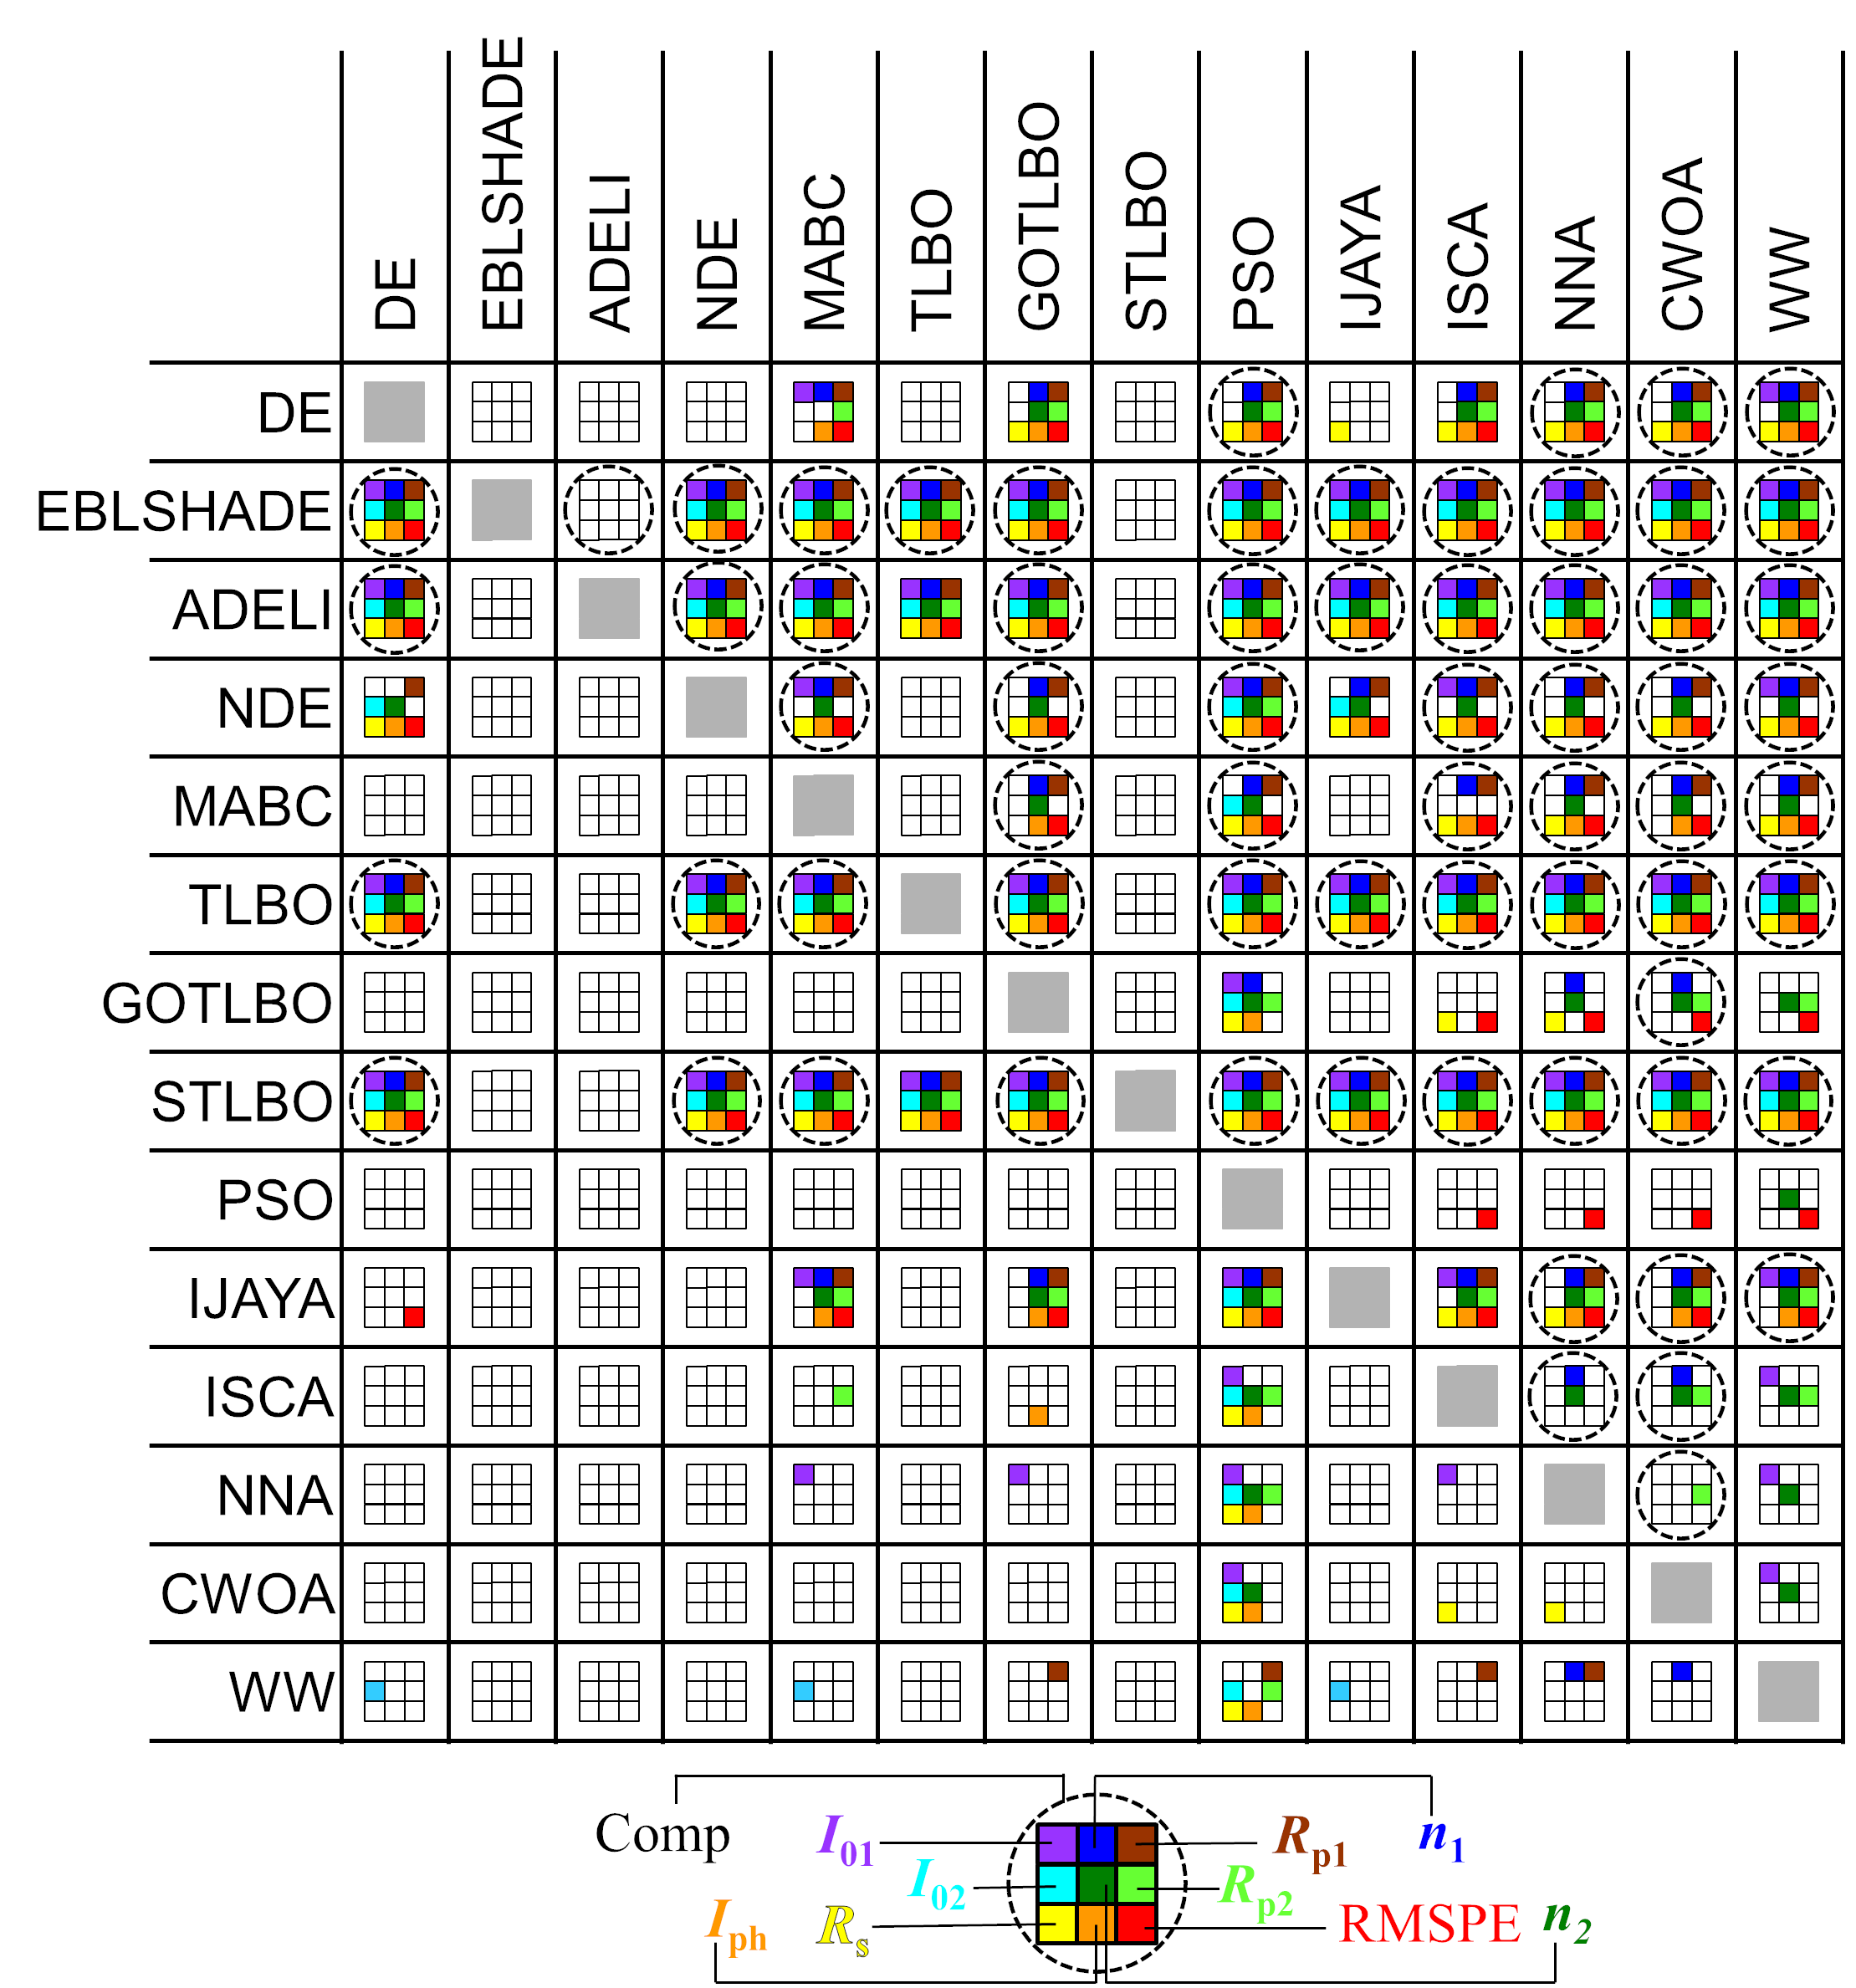
\includegraphics[width=0.45\columnwidth]{Fig5}
	  \caption{The results of Wilcoxon signed-rank test with a level of significance $\alpha = 0.05$ in the single-IV case.
               Each colored small square indicates that the algorithm specified in the row outperforms the algorithm
               specified in the column in evaluating one of the parameters of the two--diode model.
               The correspondence between the color and position of the square to a model parameter
               is shown in a legend at the figure bottom.
               The advantage of the row algorithm in the Comp parameter is indicated by the presence of a dashed circle.}\label{figWilSingleIV}
\end{figure}

\begin{figure}[]
	\centering
		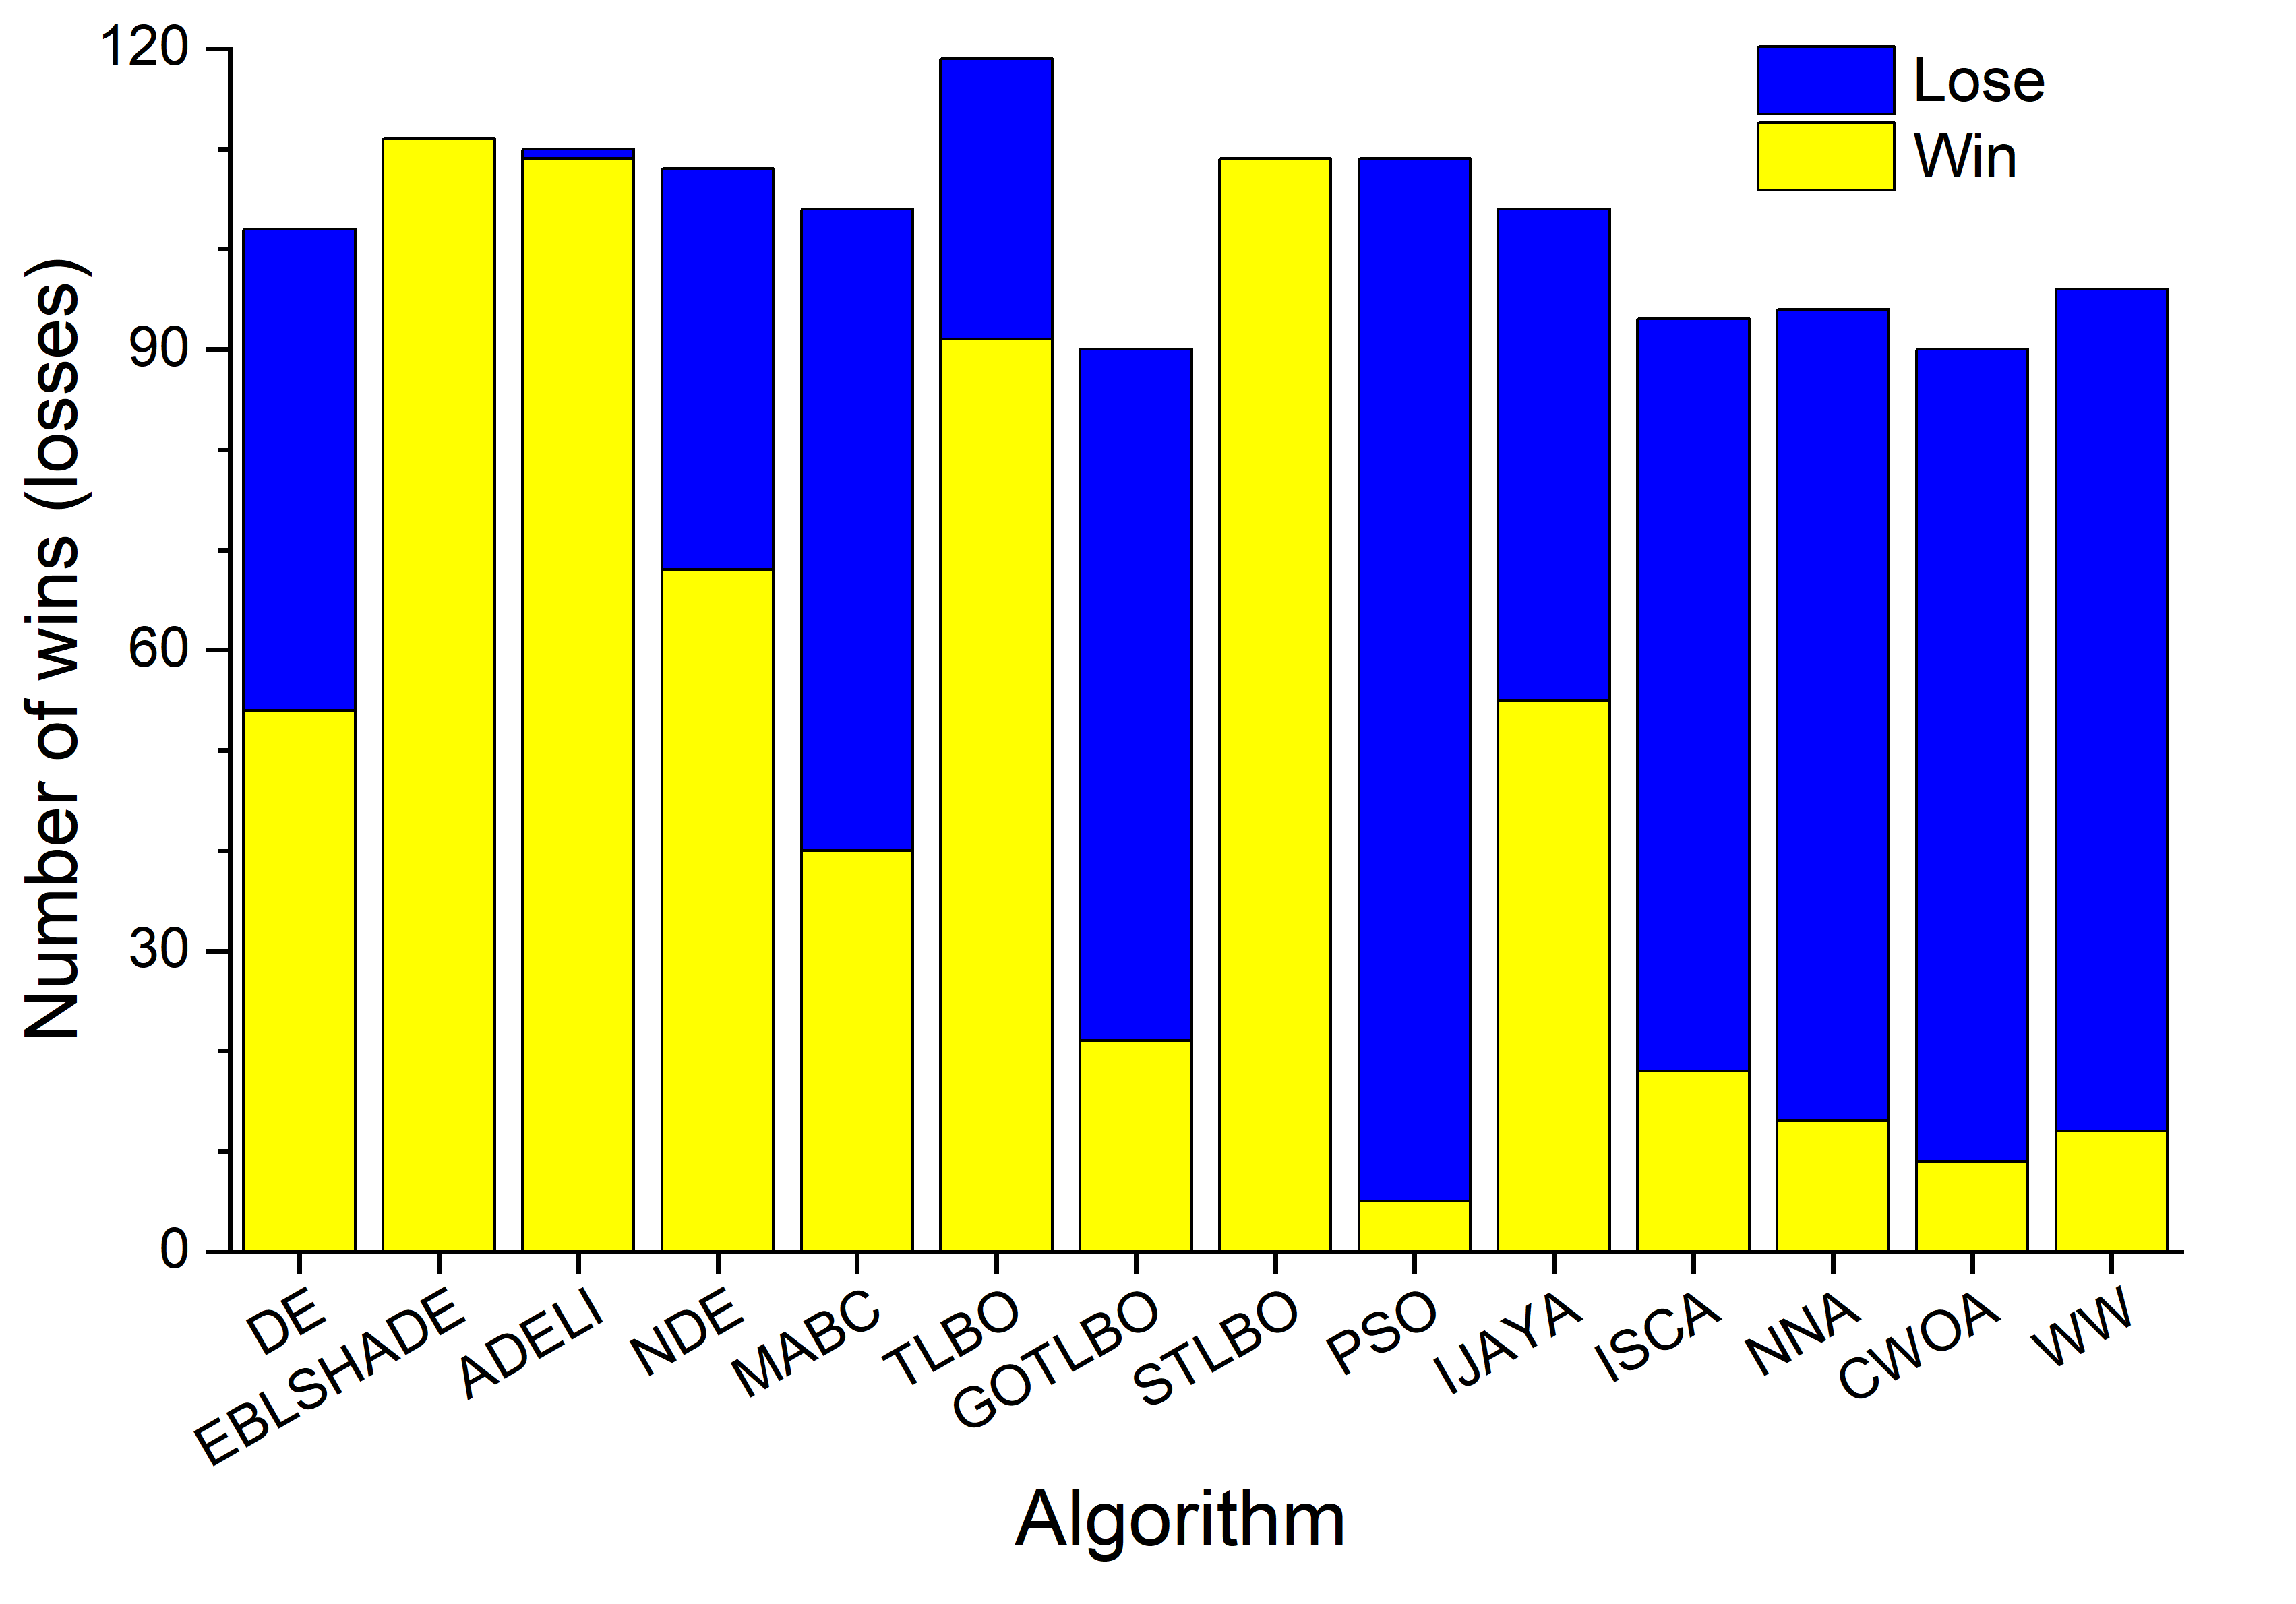
\includegraphics[width=0.45\columnwidth]{Fig6}
	  \caption{The total count of wins and losses for each algorithm in pairwise comparisons using the
               Wilcoxon signed-rank test with a significance level of $\alpha = 0.05$ in the single-IV case.}\label{figWilTotSingleIV}
\end{figure}

Fig.~\ref{figWilSingleIV} graphically depicts
the non-parametric statistical results of pairwise comparisons of the algorithms
based on the Wilcoxon signed--rank test.
For the Comp parameter comparisons, the differences in the performance scores
were normalized to the interval $[0,\, 1]$ to facilitate the comparison.
The figure shows that no single algorithm outperforms all the others in evaluating each parameter.
Furthermore, no algorithm surpasses all the others when estimating even a single parameter.


For example, as the figure states, STLBO shows a significant improvement over
DE, NDE, MABC, GOTLBO, PSO, IJAYA, ISCA, NNA, CWOA, and WW across all the parameters
considered with a level of significance $\alpha = 0.05$.
Simultaneously, no significant differences were detected between the STLBO algorithm
and both the EBLSHADE and ADELI algorithms for the estimation of all parameters.
Additionally, no significant differences were found between STLBO and TLBO for the Comp parameter comparisons.
EBLSHADE outperforms almost all other algorithms in the composite parameter except STLBO.
According to the count of victories in the Wilcoxon test,
the worst performances are exhibited by PSO and CWOA.
PSO achieved better results than ISCA, NNA, and CWOA in RMSPE value and
also outperformed WW in $n_2$ estimation and RMSPE.
Test detected significant differences between CWOA and WW in $n_2$ and $I_{01}$ estimations,
between CWOA and PSO in $I_{01}$, $I_{02}$, $R_\mathrm{s}$, and $I_\mathrm{ph}$ estimations,
and between CWOA and both ISCA and NNA in $R_\mathrm{s}$  estimation only.

Looking at the results of the Wilcoxon test from another perspective,
it can be observed that neither EBLSHADE nor STLBO suffered any defeats in pairwise comparisons,
while ADELI experienced only one loss.
ADELI was defeated in the Comp parameter only by  EBLSHADE,
primarily due to significantly longer run time.
The highest number of defeats was observed for the PSO and WW algorithms
(104 and 84, respectively).
Fig.~\ref{figWilTotSingleIV} summarizes the total number of wins and losses in the Wilcoxon test for each algorithm.



\begin{figure}[!ht]
	\centering
		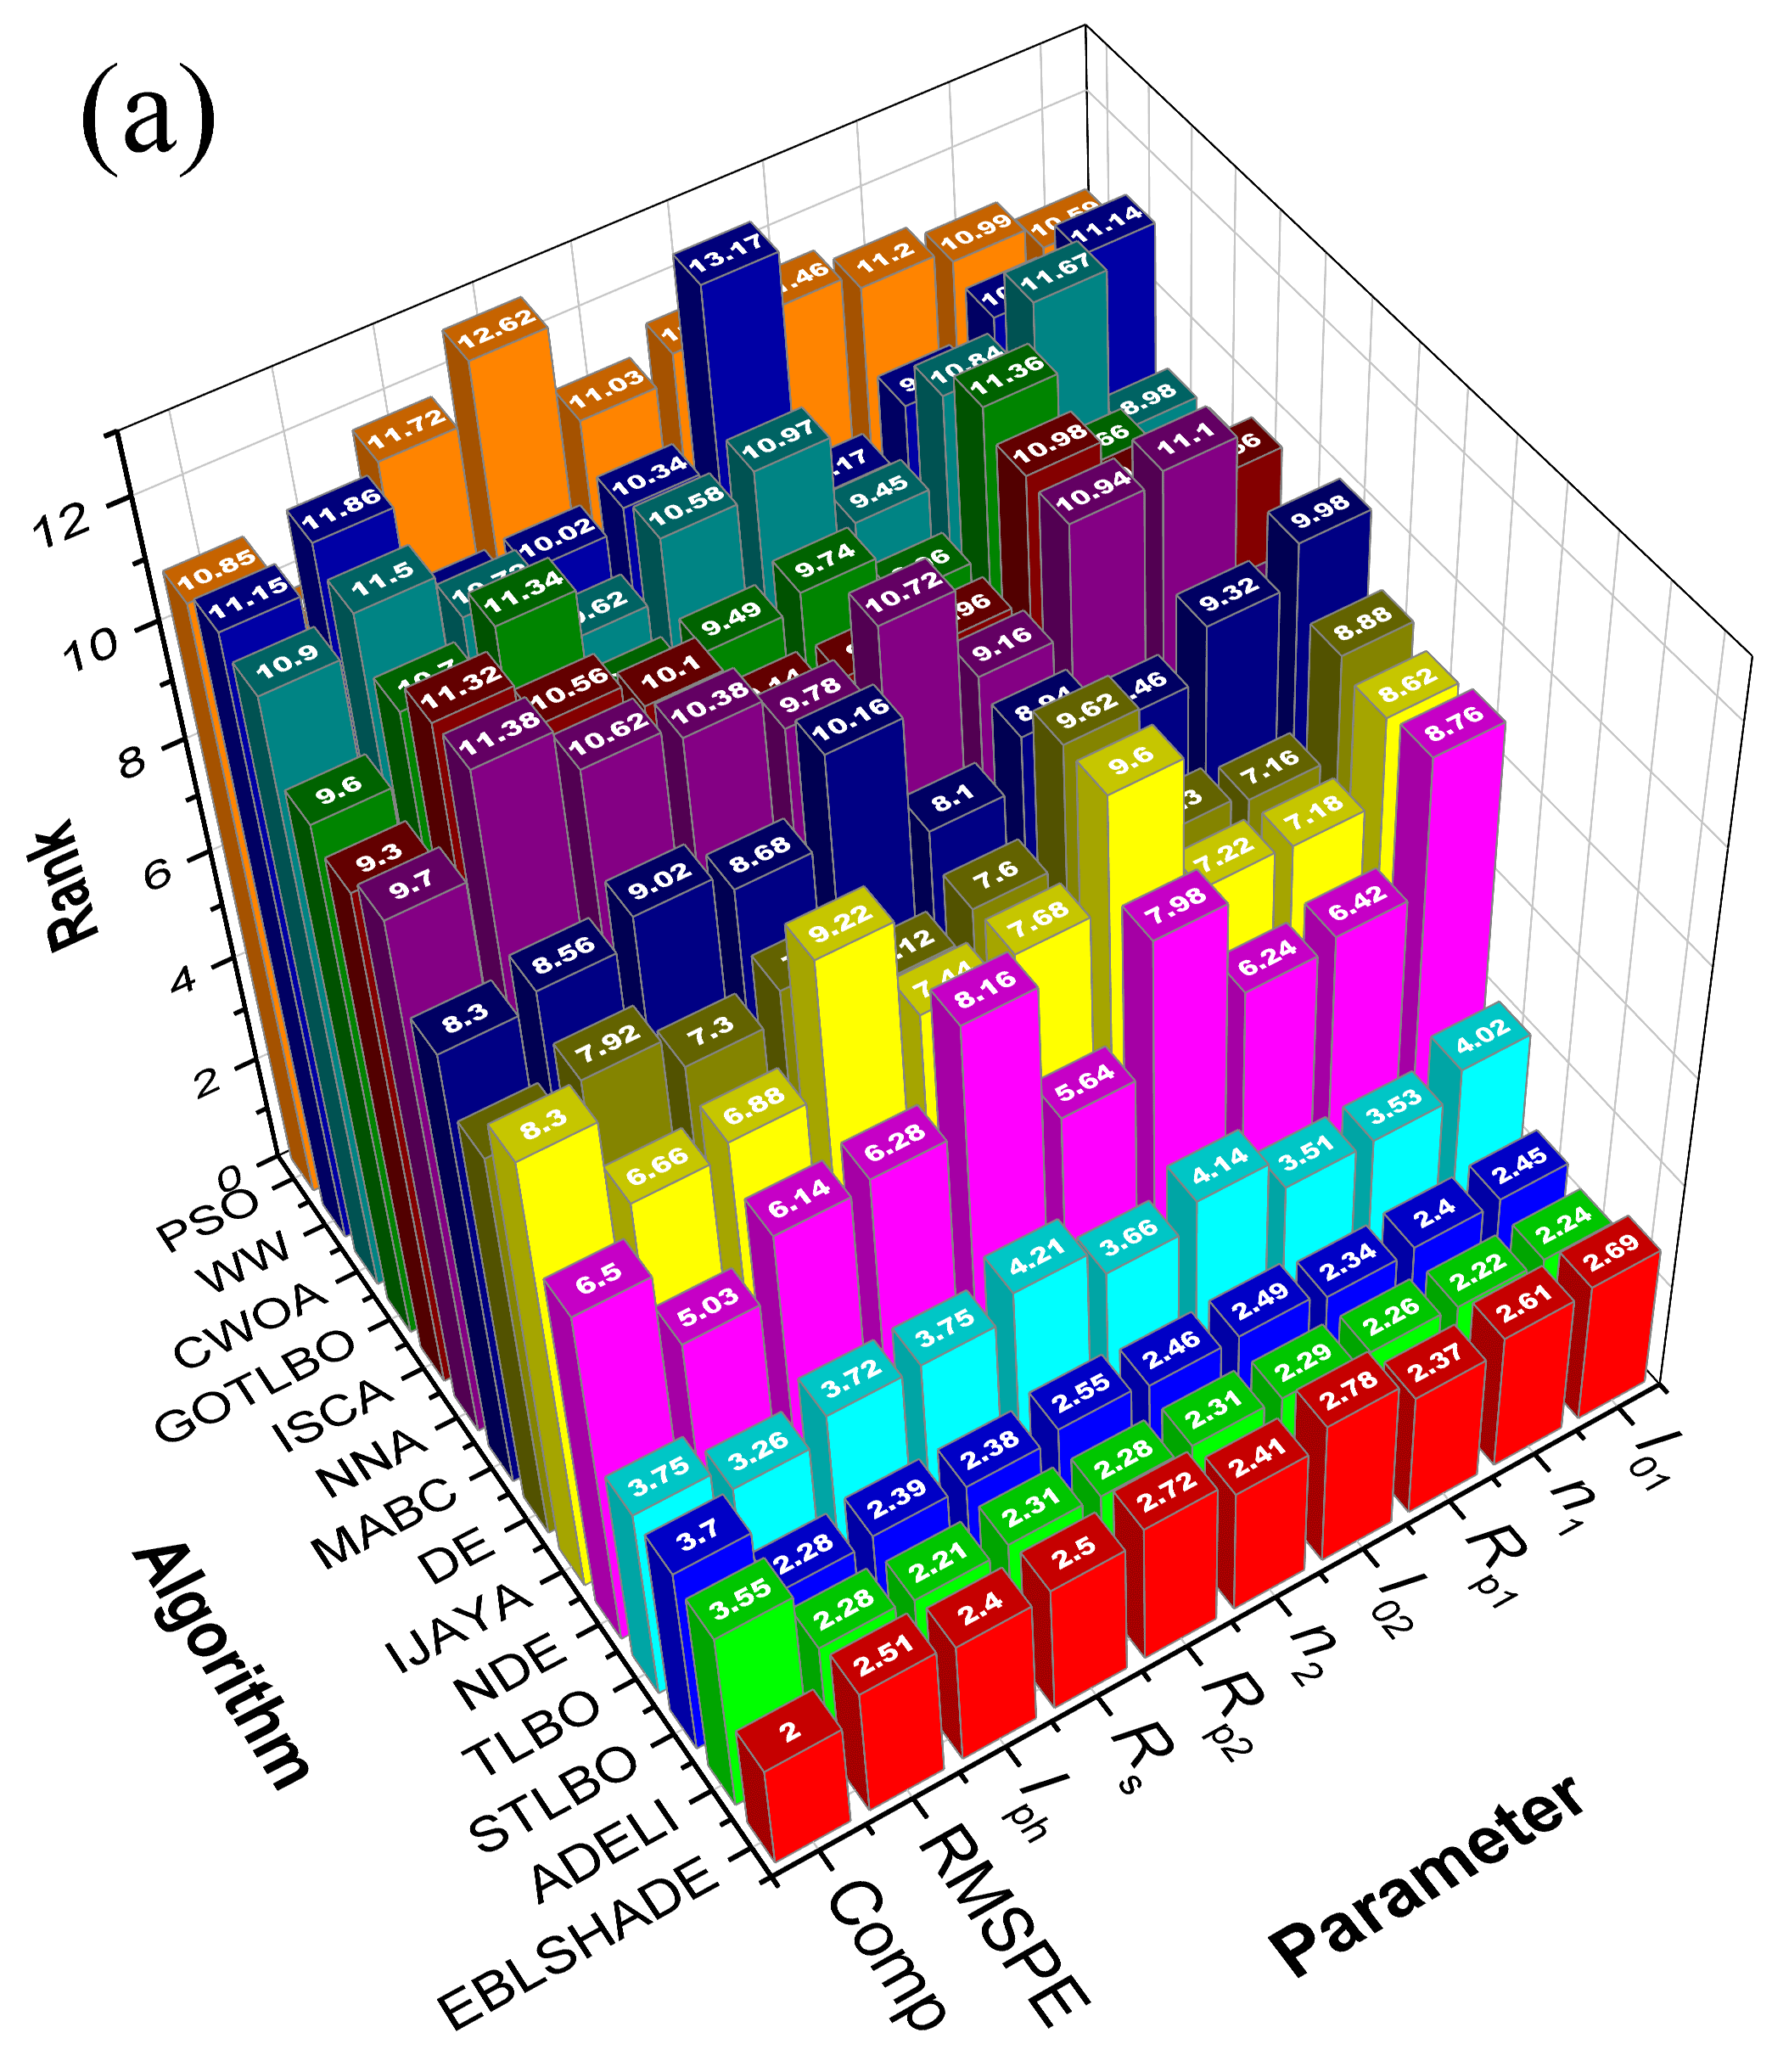
\includegraphics[width=.32\columnwidth]{Friedman}
        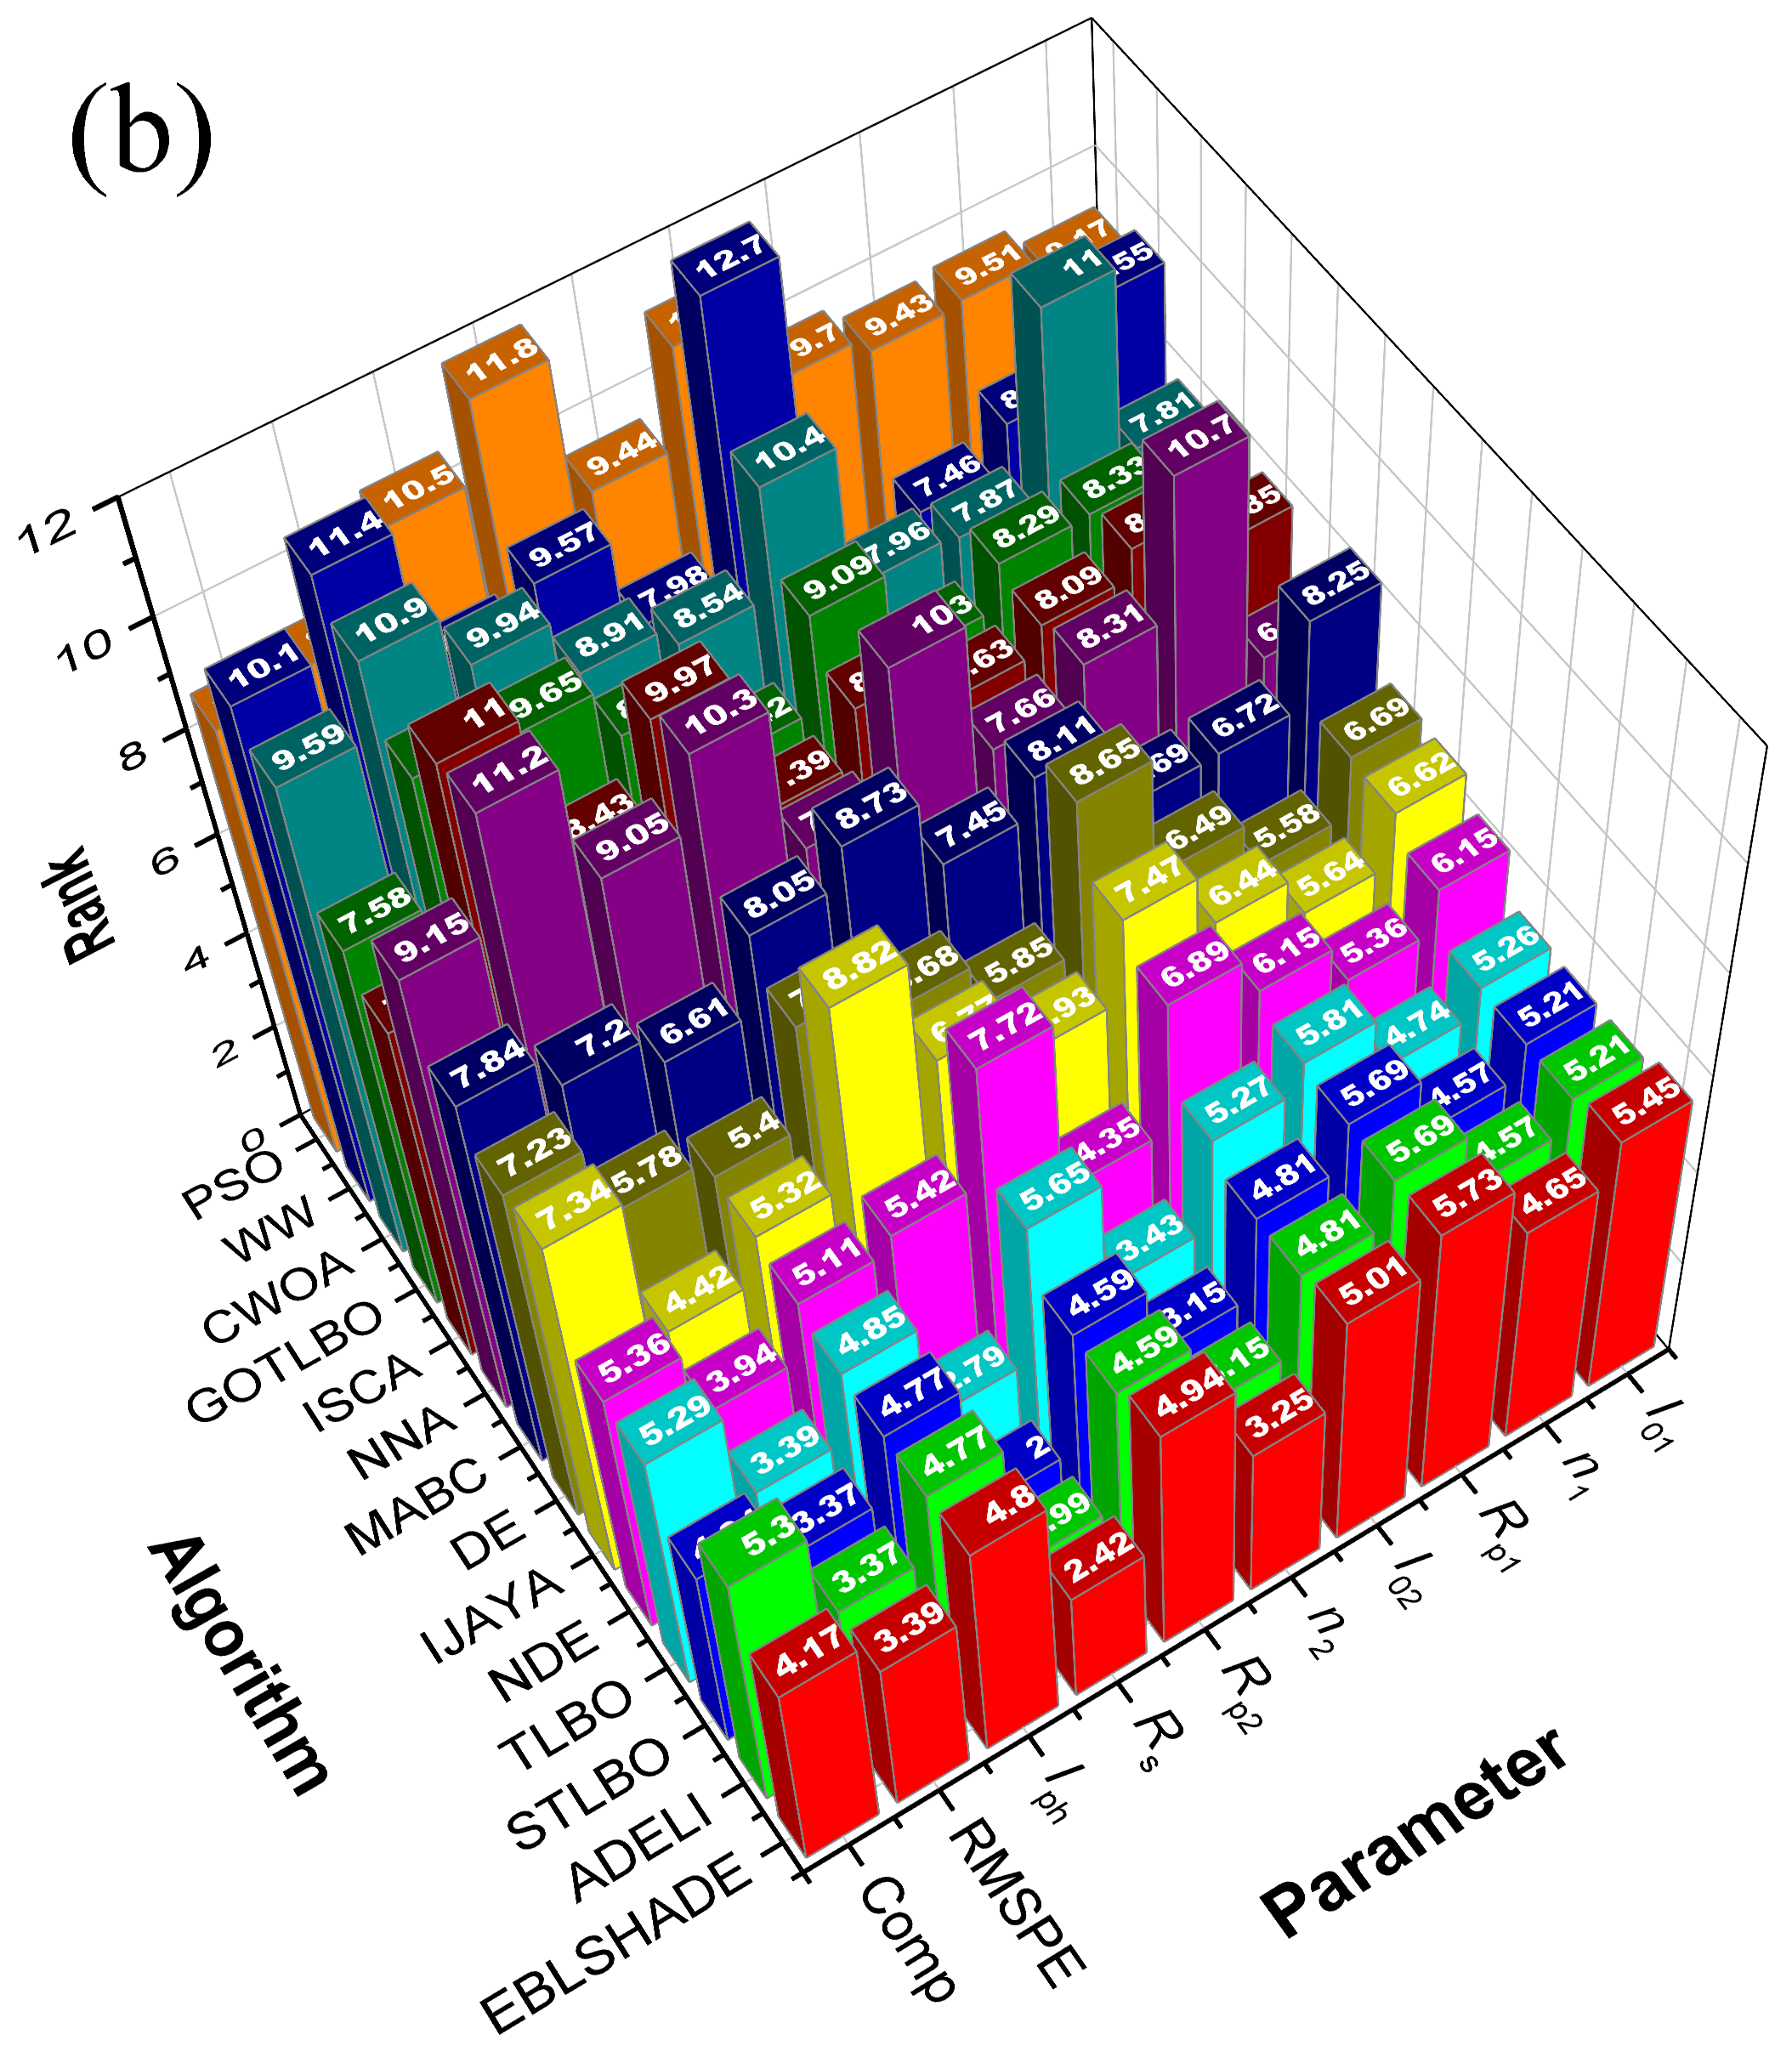
\includegraphics[width=.32\columnwidth]{FriedmanAlignedRank}
        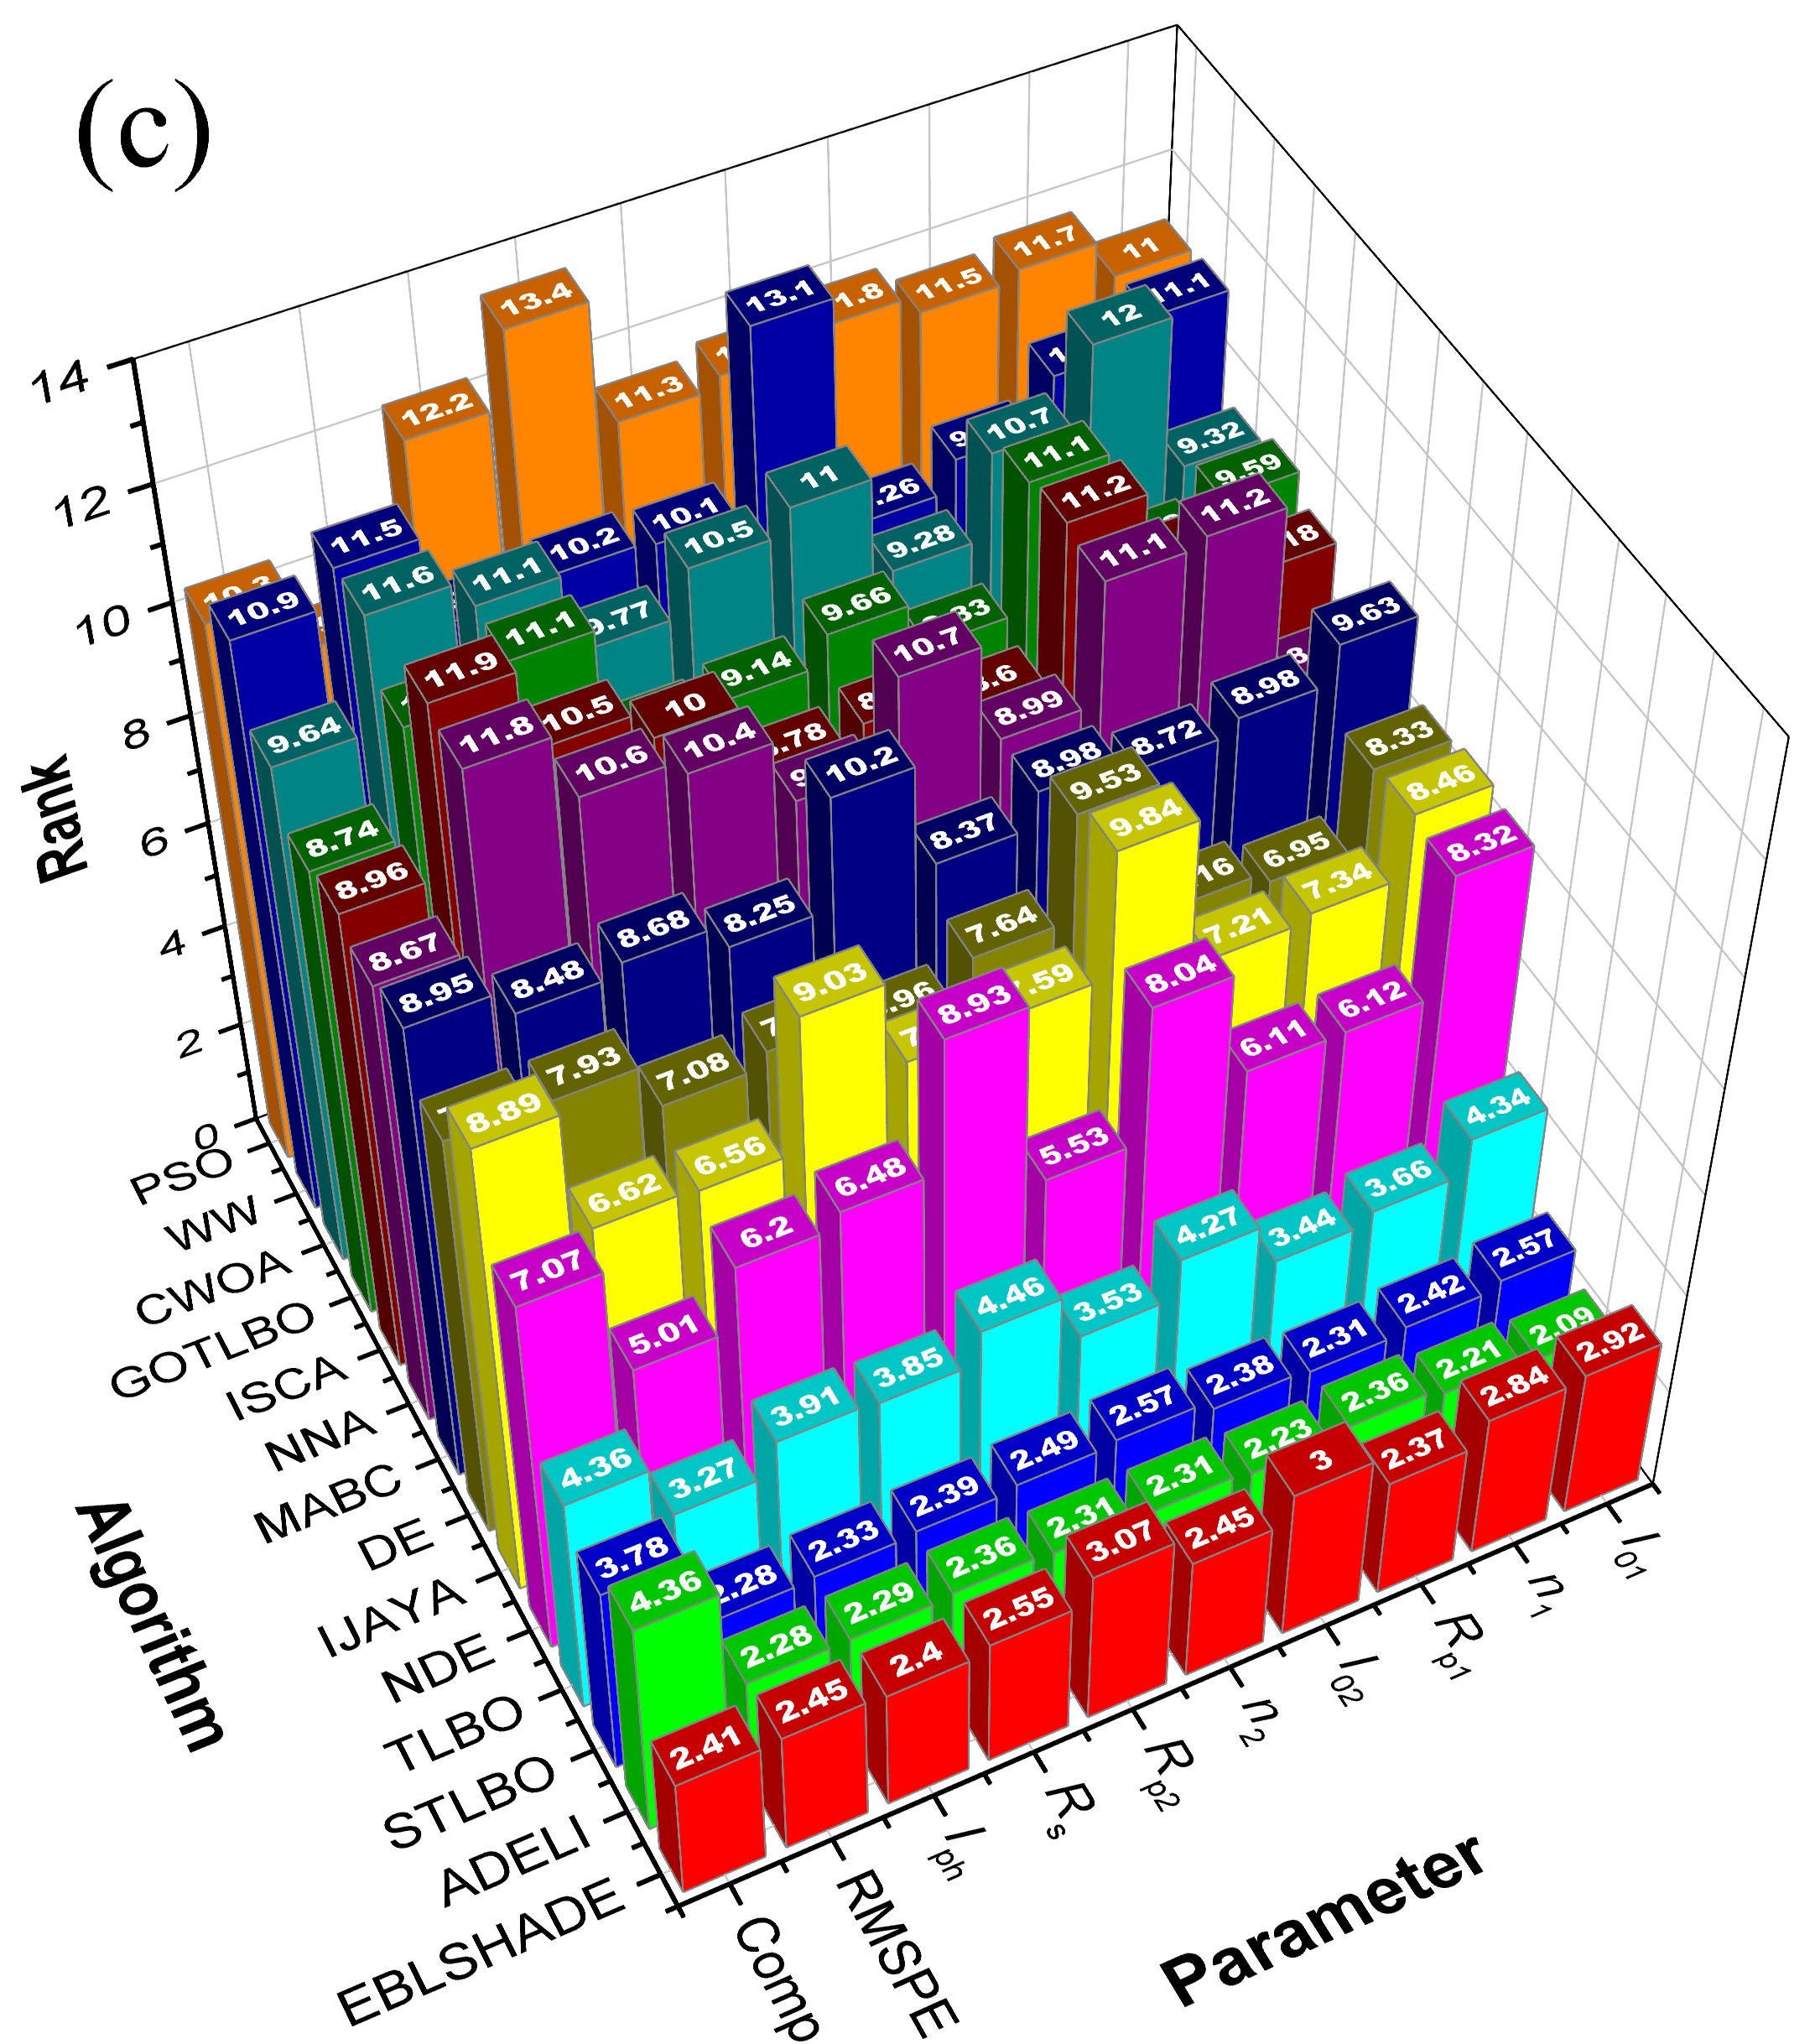
\includegraphics[width=.32\columnwidth]{QuadeRank}
	  \caption{Ranking of the algorithms according to Friedman (a), Friedman Aligned (b), and Quade (c) tests in the single-IV case.}\label{figRanksSingleIV}
\end{figure}

It is recommended \cite{Derrac2011} to initiate the multiple comparison tests by examining the null hypothesis $H_0$,
which asserts the equality of medians among the populations of results obtained by different algorithms.
The $p$--values for the null hypothesis, computed through the statistics of Friedman, Friedman Aligned,
and Quade tests and the Iman--Davenport extension, are provided in the supplementary material (table S2).
The highest observed $p(H_0)$--values were found to be $2.7\cdot10^{-5}$  (Friedman Aligned test for the task of Rp estimation),
$4.4\cdot10^{-4}$ (Friedman Aligned test for the composite parameter case),
and $8.3\cdot10^{-6}$ (Quade test, Comp parameter).
Thus, the obtained data strongly suggest the significant differences among the considered algorithms
in the accuracy of all model parameter determination, RMSPE values, and the Comp parameter.


Fig.~\ref{figRanksSingleIV} illustrates the ranks achieved
by the Friedman, Friedman Aligned, and Quade tests for the applied optimization algorithms in different tasks.
These ranks are also tabulated in the supplementary material (table S3).
In nearly all cases, the algorithms EBLSHADE, ADELI, and STLBO consistently achieve the top three ranks.
For instance, in assessing the accuracy of model parameter estimation, ADELI has ranked first  22 times.
The STLBO algorithm ranked first six times,
taking the sole first place twice ($I_{01}$ estimation according to Friedman Aligned test and
$R_\mathrm{p1}$ estimation according to Quade test)
and sharing it with ADELI four times ($n_1$, $R_\mathrm{p1}$, $n_2$, and $I_\mathrm{ph}$
estimation according to Friedman Aligned test).
In the RMSPE  case, ADELI and STLBO attained equal and top ranks across all three tests utilized.
When comparing based on the Comp parameter,
the STLBO algorithm secured the top rank according to the Friedman Aligned test,
whereas the Friedman and Quade tests identified EBLSHADE as the best performer.
For the most part, the TLBO algorithm consistently ranked fourth among all the tested algorithms.
Interestingly, in four cases ($I_{01}$ estimation, RMSPE value, and Comp parameter by Friedman Aligned test,
and Comp parameter by Quade test),
it even achieved a commendable third-place ranking.
We must note that overall, the absolute values of ranks for the ADELI, STLBO, EBLSHADE,
and TLBO algorithms differ only slightly, and the difference between the first and fourth ranks is often less than 0.5.
The worst ranks are observed for PSO, NNA, CWOA, and WW.

It is known \cite{Derrac2011} that
the Friedman, Friedman Aligned, and Quade tests are inadequate for establishing accurate comparisons between the considered algorithms.
To compare a control method (one of 14 tested)
with a set of other algorithms (the remaining 13),
one can define a family of null hypotheses related to the control method.
Applying a post-hoc procedure makes it possible to obtain a $p$--value that indicates
the probability of obtaining the observed results if the corresponding hypothesis is true.
We calculated $p$--values using four post-hoc procedures (Finner, Holm, Hochberg, and Holland) for all algorithms, tests, and tasks.
The reader is referred to the supplementary material for all $p$-values (Tables S4-S143).
In particular, a common feature of all comparisons is that
the Finner post-hoc procedure demonstrates the most powerful behavior, yielding the lowest $p$--values.


In our study, we adopted a threshold value of $p_{cr}=0.1$
to establish a critical level for comparing the algorithms' effectiveness
in both multiple $1\times N$  and $N\times N$ comparisons.
That is, it was defined that the likelihood of obtaining a result as extreme as the observed one
if there is no difference between the two algorithms (null hypothesis), was less than 10\%.



\begin{table*}[<options>]
\caption{The total count of wins and losses for each algorithm in $1\times N$ multiple comparisons using the
Friedman, Friedman Aligned, and Quade tests and Finner, Holm, Hochberg, and Holland post-hoc procedures
in single--IV case.
The criterion for victory was a adjusted $p$-value less than 0.1.
}\label{tbl1NWins}
\begin{tabular*}{\tblwidth}{@{}LCCCCCCCCCCC@{}}
\toprule
\multirow{3}{*}{Algorithm}& \multicolumn{11}{C}{Wins / Loses} \\
&  \multicolumn{10}{C}{task}  &\multirow{2}{*}{Total}\\
  & $I_{01}$& $n_1$ & $R_\mathrm{p1}$ &$I_{02}$& $n_2$& $R_\mathrm{p2}$&$R_\mathrm{s}$&$I_\mathrm{ph}$&RMSPE&Comp&\\ % Table header row
\midrule
DE & 24/43 & 56/34 & 48/35 &  4/73 & 48/43 & 49/34 & 49/40  & 45/35  & 49/48 & 16/27  & 388/412\\
EBLSHADE & 108/\textbf{0} & 108/\textbf{0}  & \textbf{107}/\textbf{0}  & 103/\textbf{0}  & 107/\textbf{0}  & 104/\textbf{0}  & 111/2  & \textbf{105}/\textbf{0}  &  \textbf{109}/\textbf{0}& \textbf{88}/\textbf{0}  & 1050/2 \\
ADELI & \textbf{122}/\textbf{0} & \textbf{110}/\textbf{0}  &  \textbf{107}/\textbf{0} &  \textbf{128}/\textbf{0} &  \textbf{110}/\textbf{0} &  \textbf{122}/\textbf{0} & \textbf{119}/\textbf{0}  & \textbf{105}/\textbf{0}  &  \textbf{109}/\textbf{0}& 61/2  & \textbf{1093}/2\\
NDE & 35/19  & 56/32  & 56/19  & 36/49  & 77/32  & 23/45  &  73/32 & 48/8 & 83/29 & 23/20  & 519/285\\
MABC &  8/61 & 28/69 & 44/45  &  9/57 & 40/55  & 4/82  & 32/51  & 32/66  & 44/62 & 8/30  & 249/578\\
TLBO & 80/3 & 102/\textbf{0} & 101/\textbf{0} &  84/13&  99/\textbf{0}& 87/18 & 93/10 & 94/\textbf{0} & 100/\textbf{0} & 65/2  & 905/46\\
GOTLBO & 8/60  & 12/73  & 4/84  & 16/49  & 20/74  & 13/54 & 20/61  & 4/80 & 16/85  & 13/28  & 126/648\\
STLBO & 109/\textbf{0} & \textbf{110}/\textbf{0}  & \textbf{107}/\textbf{0}  & 125/\textbf{0}  & 107/\textbf{0}  & 119/\textbf{0}  & 116/\textbf{0}  & \textbf{105}/\textbf{0}  & \textbf{109}/\textbf{0} & 81/\textbf{0}  & 1088/\textbf{0}\\
PSO & 0/84  & 8/88  & 0/100  & 0/108  & 4/101  & 0/96  &  0/124 & 0/96  & 20/70  & 4/49  & 72/916\\
IJAYA &  28/28 &  56/34 &  48/35 & 13/52  & 45/43 &  54/34 &  20/61 & 56/29  & 57/38  & 16/34  & 393/388\\
ISCA & 8/56  & 12/76  & 4/84  & 12/45  & 28/65  & 16/51  & 8/61  & 17/68  & 0/92  & 16/32  & 121/630\\
NNA & 33/29  & 0/92  & 4/84  & 12/49  & 12/84  & 12/57  & 8/77  & 12/80  & 0/92& 0/52  & 93/696\\
CWOA & 8/60  & 0/96  &  4/80& 8/52  & 8/84& 4/83  & 20/61  & 0/88  & 0/92 & 0/52  & 52/748\\
WW & 0/96  & 12/76  & 16/76&  36/43 & 0/108 & 10/60 & 12/77  & 12/66  & 0/92& 0/52  & 98/844\\
\bottomrule
\end{tabular*}
\end{table*}


The statistical results of the comparison of algorithm effectiveness are available in the supplementary materials (figure S3).
Among the compared algorithms, EBLSHADE, ADELI, and STLBO consistently outperform the others in $1\times N$ multiple comparisons.
On the other hand, algorithms such as PSO, ISCA, CWOA, and NNA consistently yield lower-quality results.
The main changes observed in nonparametric statistical estimation of different parameters evaluation
mainly concern algorithms with moderate effectiveness.



In all cases, the Quade test yields higher adjusted $p$-values.
In particular, in the case of the complex parameter, the $p$-value for any comparison did not exceed the chosen threshold value $p_{cr}$.



The adjusted $p$--values obtained from the direct comparisons of EBLSHADE, ADELI, and STLBO
do not allow us to determine the best algorithm among them.
However, we can use the results of these top three algorithms,
obtained from their comparisons with less efficient optimization methods, for this purpose.
Table~\ref{tbl1NWins} summarizes the counts of wins and losses for each algorithm in $1\times N$ multiple comparisons.
The maximum possible number of wins achieved in every 10 tasks is 156,
obtained from comparisons with 13 algorithms across 3 tests using 4 procedures.
Among the compared algorithms, ADELI showed the highest number of statistically
significant improvements (1093) over others,
indicating its superior performance.
Conversely, STLBO demonstrated the lowest number of defeats (0)
in similar comparisons, suggesting its consistently strong performance.


The results above show the outcomes of the procedures used to control the Family-Wise Error Rate (FWER)
for comparisons with a control algorithm.
We individually tested each of the 14 algorithms to determine if any of them were superior to the others.
The results below display the multiple comparisons carried out,
involving the computation of all possible pairwise comparisons ($N\times N$ comparison).
Three procedures (Shaffer’s static, Nemenyi, and Holm) were employed to control FWER.
These procedures consider that the hypotheses being tested belong to a family of all
pairwise comparisons and are logically interrelated; thus,
not all combinations of true and false hypotheses are possible.

Starting from the analysis performed by the Friedman test on our results, 
we can raise the 91 null hypotheses of equality among 
the 14 algorithms in our study for each task and apply the previously mentioned methods to contrast them.

Starting from the analysis performed by the Friedman test over our results, we can raise the
91 hypotheses of equality among the 14 algorithms of our study for each task,
and apply the methods mentioned earlier to contrast them.
Table~\ref{tblNNpValueI01} lists a portion of the hypotheses and the 
adjusted $p$-values achieved for the task of $I_{01}$ estimation.
For the remaining 46 hypotheses not indicated in the table,
a $p$-value of 1 was obtained after applying each of the procedures.
The full version of the table, as well as the data obtained for other tasks, 
are given in the supplementary material (tables S144-S153).


\begin{table*}[<options>]
\caption{Adjusted $p$-values for tests for $N\times N$ multiple comparisons of $I_{01}$ estimation
         among all methods in the single--IV case ($p<1.0$ are only shown).}\label{tblNNpValueI01}
\begin{tabular*}{\tblwidth}{@{}LCCC@{}}
\toprule
\multirow{2}{*}{Hypothesis}& \multicolumn{3}{C}{post-hoc procedure} \\
  &Nemenyi & Holm & Shaffer\\ % Table header row
\midrule
ADELI versus WW&<1E-13&<1E-13&<1E-13\\
ADELI versus NDE&1.17195E-12&1.15907E-12&1.00453E-12\\
STLBO versus CWOA&1.17195E-12&1.15907E-12&1.00453E-12\\
TLBO versus PSO&1.21236E-12&1.17240E-12&1.03917E-12\\
STLBO versus GOTLBO&1.21236E-12&1.17240E-12&1.03917E-12\\
ADELI versus DE&1.73772E-12&1.64224E-12&1.48948E-12\\
STLBO versus DE&1.83875E-12&1.71752E-12&1.57607E-12\\
ADELI versus CWOA&3.83915E-12&3.50164E-12&3.29070E-12\\
EBLSHADE versus GOTLBO&4.20286E-12&3.78719E-12&3.60245E-12\\
STLBO versus NDE&5.01110E-12&4.46043E-12&4.29523E-12\\
ADELI versus GOTLBO&5.41522E-12&4.76064E-12&4.64162E-12\\
EBLSHADE versus CWOA&5.98099E-12&5.19229E-12&5.12657E-12\\
EBLSHADE versus ISCA&1.17195E-11&1.00453E-11&1.00453E-11\\
EBLSHADE versus DE&1.45282E-11&1.22931E-11&1.06966E-11\\
EBLSHADE versus NDE&4.17053E-11&3.43725E-11&3.07061E-11\\
STLBO versus ISCA&8.17133E-11&6.64482E-11&6.01625E-11\\
TLBO versus WW&8.82197E-11&7.07696E-11&6.49529E-11\\
TLBO versus MABC&1.07900E-10&8.53717E-11&7.94431E-11\\
EBLSHADE versus MABC&3.09961E-10&2.38431E-10&2.28213E-10\\
ADELI versus NNA&3.24570E-10&2.46102E-10&2.38969E-10\\
ADELI versus ISCA&3.83410E-10&2.86504E-10&2.82291E-10\\
STLBO versus MABC&1.58351E-09&1.16588E-09&1.16588E-09\\
STLBO versus NNA&1.83408E-09&1.33021E-09&1.33021E-09\\
TLBO versus ISCA&3.49326E-09&2.49519E-09&2.22648E-09\\
ADELI versus MABC&5.83612E-09&4.10452E-09&3.71972E-09\\
EBLSHADE versus NNA&1.23520E-08&8.55140E-09&7.87272E-09\\
EBLSHADE versus PSO&1.47150E-08&1.00256E-08&9.37877E-09\\
STLBO versus PSO&5.32586E-08&3.57008E-08&3.39450E-08\\
ADELI versus PSO&1.50038E-07&9.89261E-08&.56286E-08\\
TLBO versus GOTLBO&2.16253E-07&1.40208E-07&1.37831E-07\\
EBLSHADE versus WW&2.39169E-07&1.52438E-07&1.52438E-07\\
TLBO versus CWOA&2.89034E-07&1.81043E-07&1.77867E-07\\
TLBO versus DE&5.91345E-07&3.63905E-07&3.63905E-07\\
STLBO versus WW&6.86296E-07&4.14794E-07&4.14794E-07\\
TLBO versus NDE&1.37158E-06&8.13904E-07&7.68687E-07\\
TLBO versus NNA&1.17758E-04&6.72904E-05&6.59964E-05\\
NNA versus WW&2.21281E-02&1.24015E-02&1.24015E-02\\
IJAYA versus WW&2.36193E-01&1.29777E-01&1.24585E-01\\
NNA versus PSO&2.36193E-01&1.29777E-01&1.24585E-01\\
NDE versus WW&4.04596E-01&2.13413E-01&2.13413E-01\\
DE versus WW&6.28685E-01&3.24706E-01&3.24706E-01\\
CWOA versus WW&8.94683E-01&4.52257E-01&4.52257E-01\\
GOTLBO versus WW&1.0&5.07626E-01&5.07626E-01\\
IJAYA versus PSO&1.0&8.15876E-01&7.97333E-01\\
NNA versus MABC&1.0&9.64793E-01&9.64793E-01\\
\bottomrule
\end{tabular*}
\end{table*}



It can be seen that at a significance level of 0.1, 
only 37 hypotheses of equality are rejected by the Nemenyi, Holm, and Shaffer methods.
These hypotheses show the improvement of EBLSHADE, ADELI, TLBO, and STLBO 
over DE, NDE, MABC, GOTLBO, PSO, ISCA, NNA, CWOA, and WW, 
as well as NNA over WW. 
None of the remaining 54 hypotheses can be rejected using these procedures.


It should be noted that when testing complementary hypotheses 
(``algorithm A vs algorithm B'' and ``algorithm B vs algorithm A''), 
a $p$--value less than 1 can be obtained in only one of the two cases.
For instance, when using the Nemenyi procedure to $I_{01}$ evaluating by comparing ``ADELI vs MABC'', 
a $p$--value of $5.84\cdot10^{-9}$ was obtained. 
Conversely, when comparing ``MABC vs ADELI'', the $p$--value was 1.
The $p$-values were computed for all possible hypotheses in the study to identify algorithms whose results statistically deviate from those of other algorithms.
In this case, a critical value of $p_{cr}=0.1$ was used, similar to the $1\times N$ multiple comparisons.
Typical examples of the obtained results for specific parameter cases are presented in Fig.~\ref{figNNRezSingleIV}.
Please refer to figure S4 in the supplementary materials for more detailed and comprehensive data.
Generalized results regarding the total count of victories and defeats in the $N\times N$ comparisons 
are listed in Table~\ref{tblNNWins}.
 In the case of $N\times N$ comparisons, the maximum possible number of wins achieved in every 10 tasks is 39, 
obtained from comparing 13 algorithms in 3 post-hoc procedures.


\begin{figure*}[!ht]
	\centering
		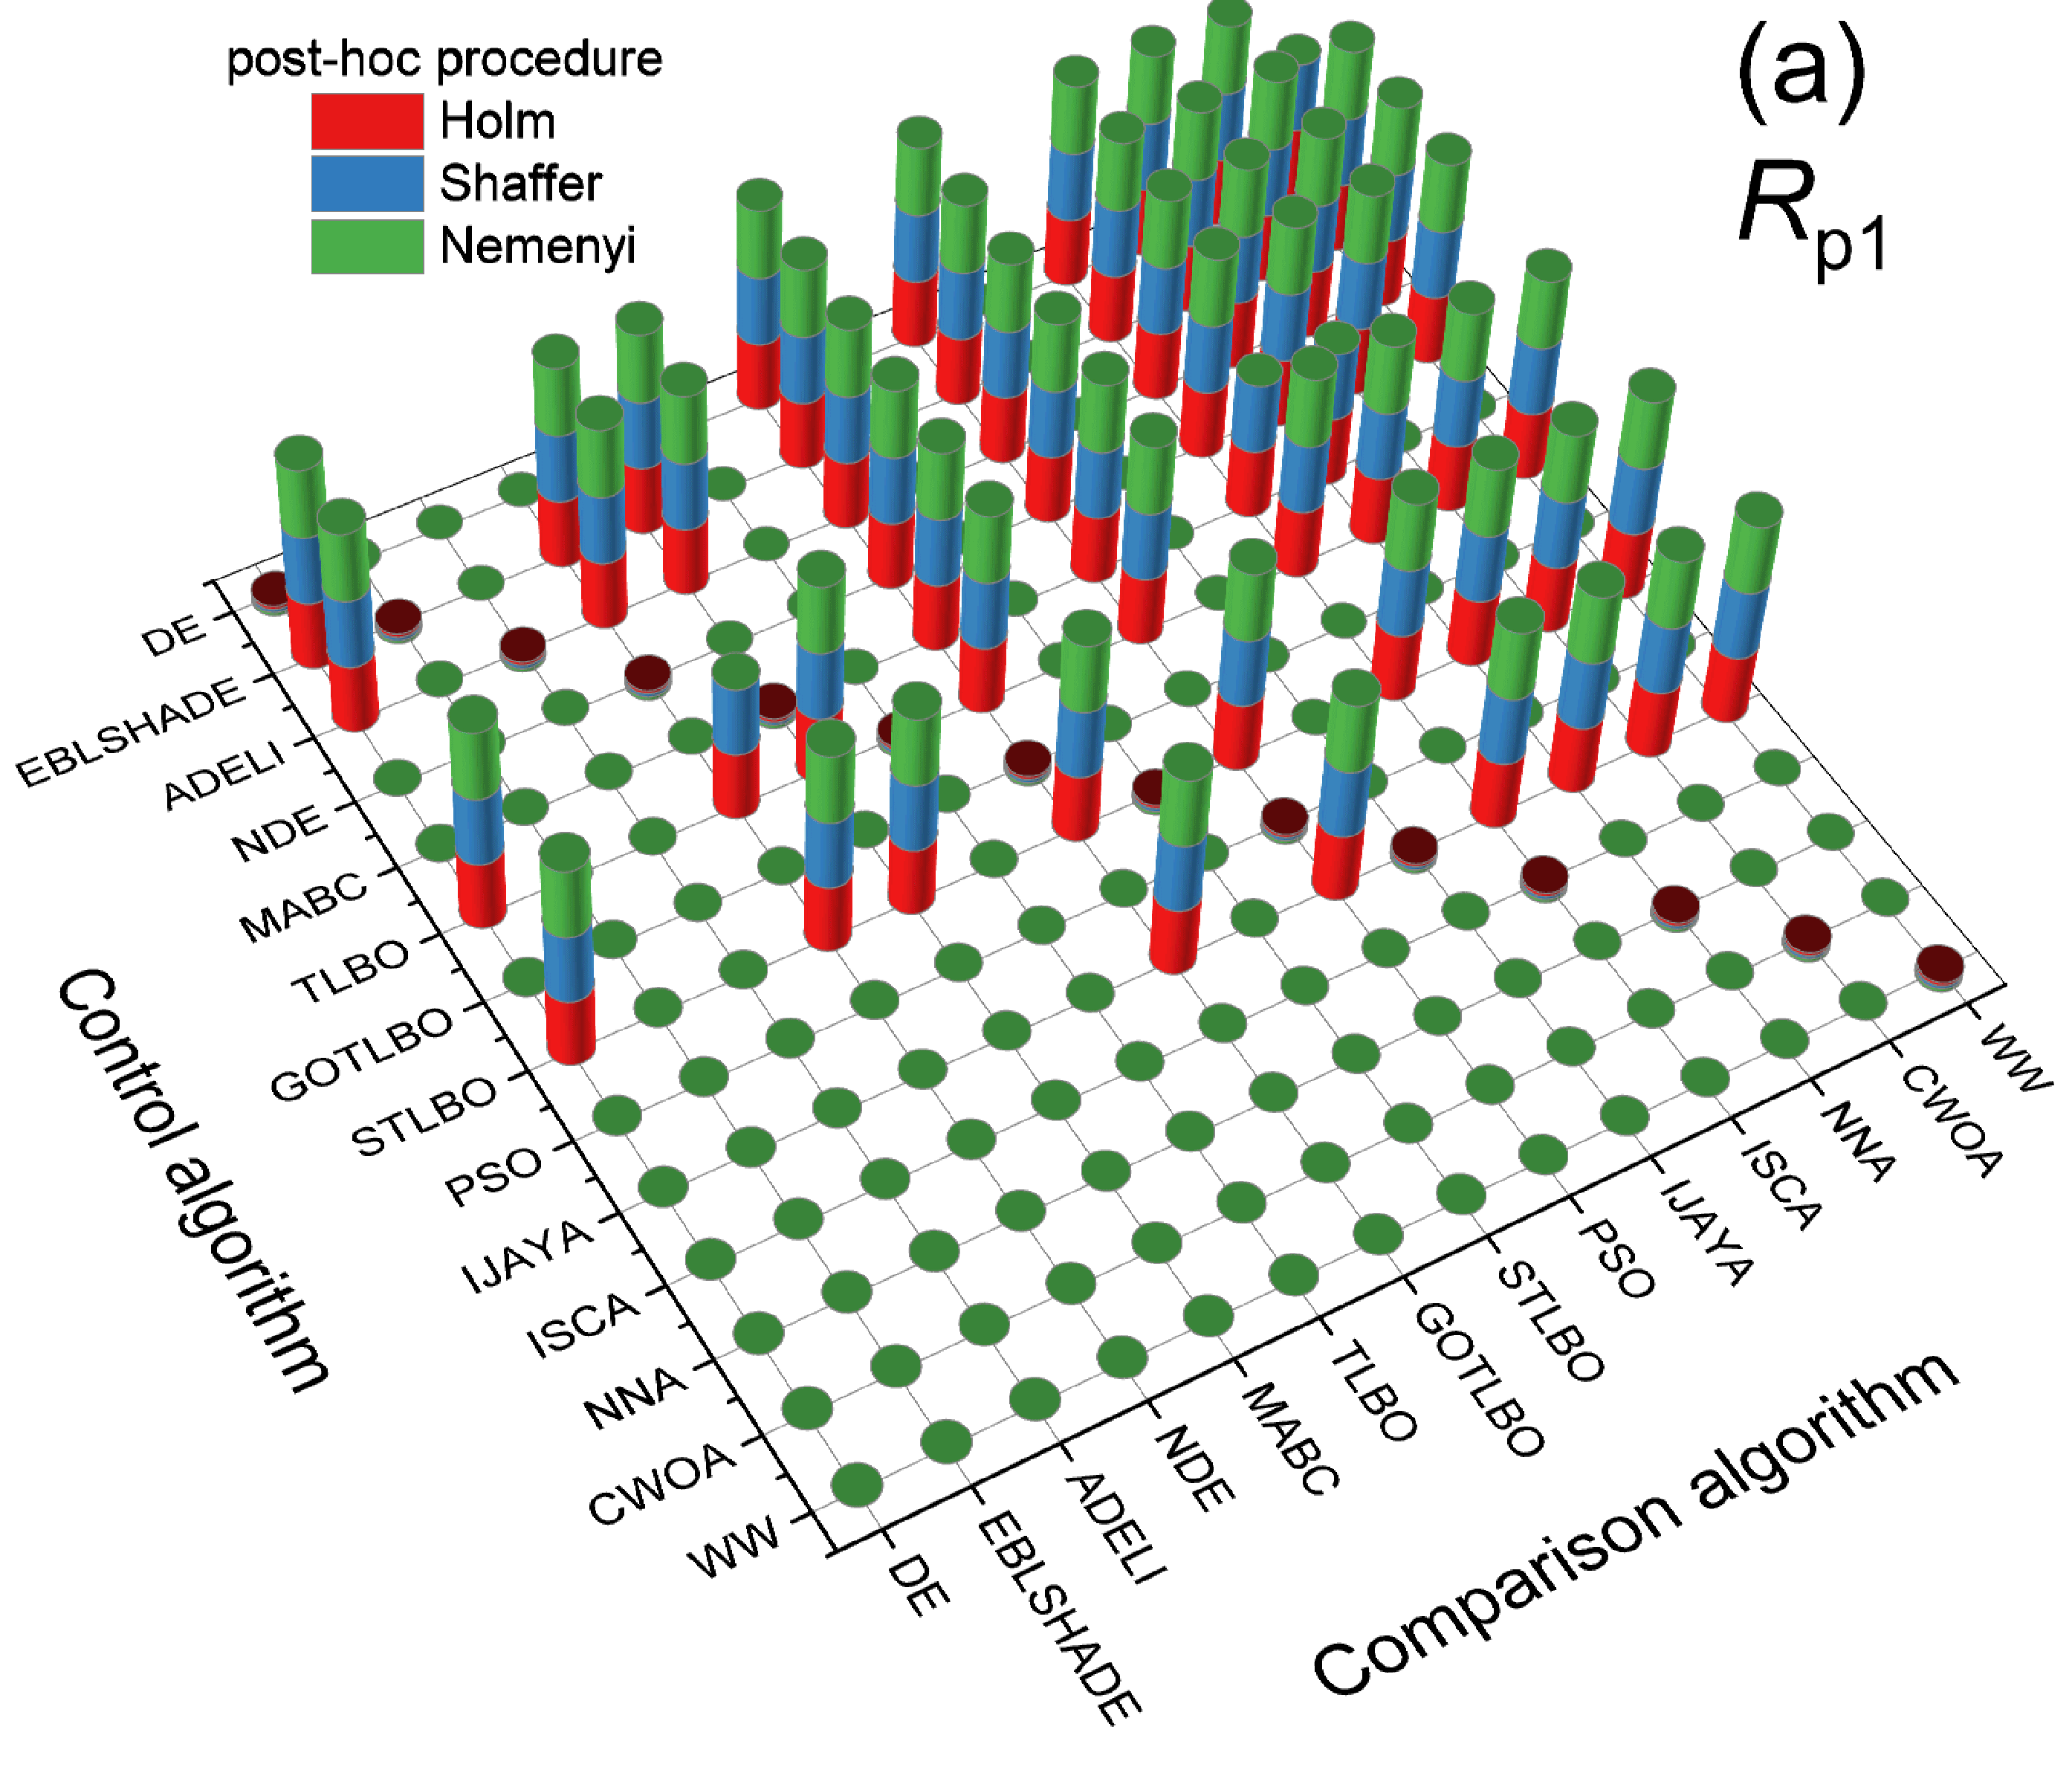
\includegraphics[width=.49\textwidth]{Rp1shot_NN}
        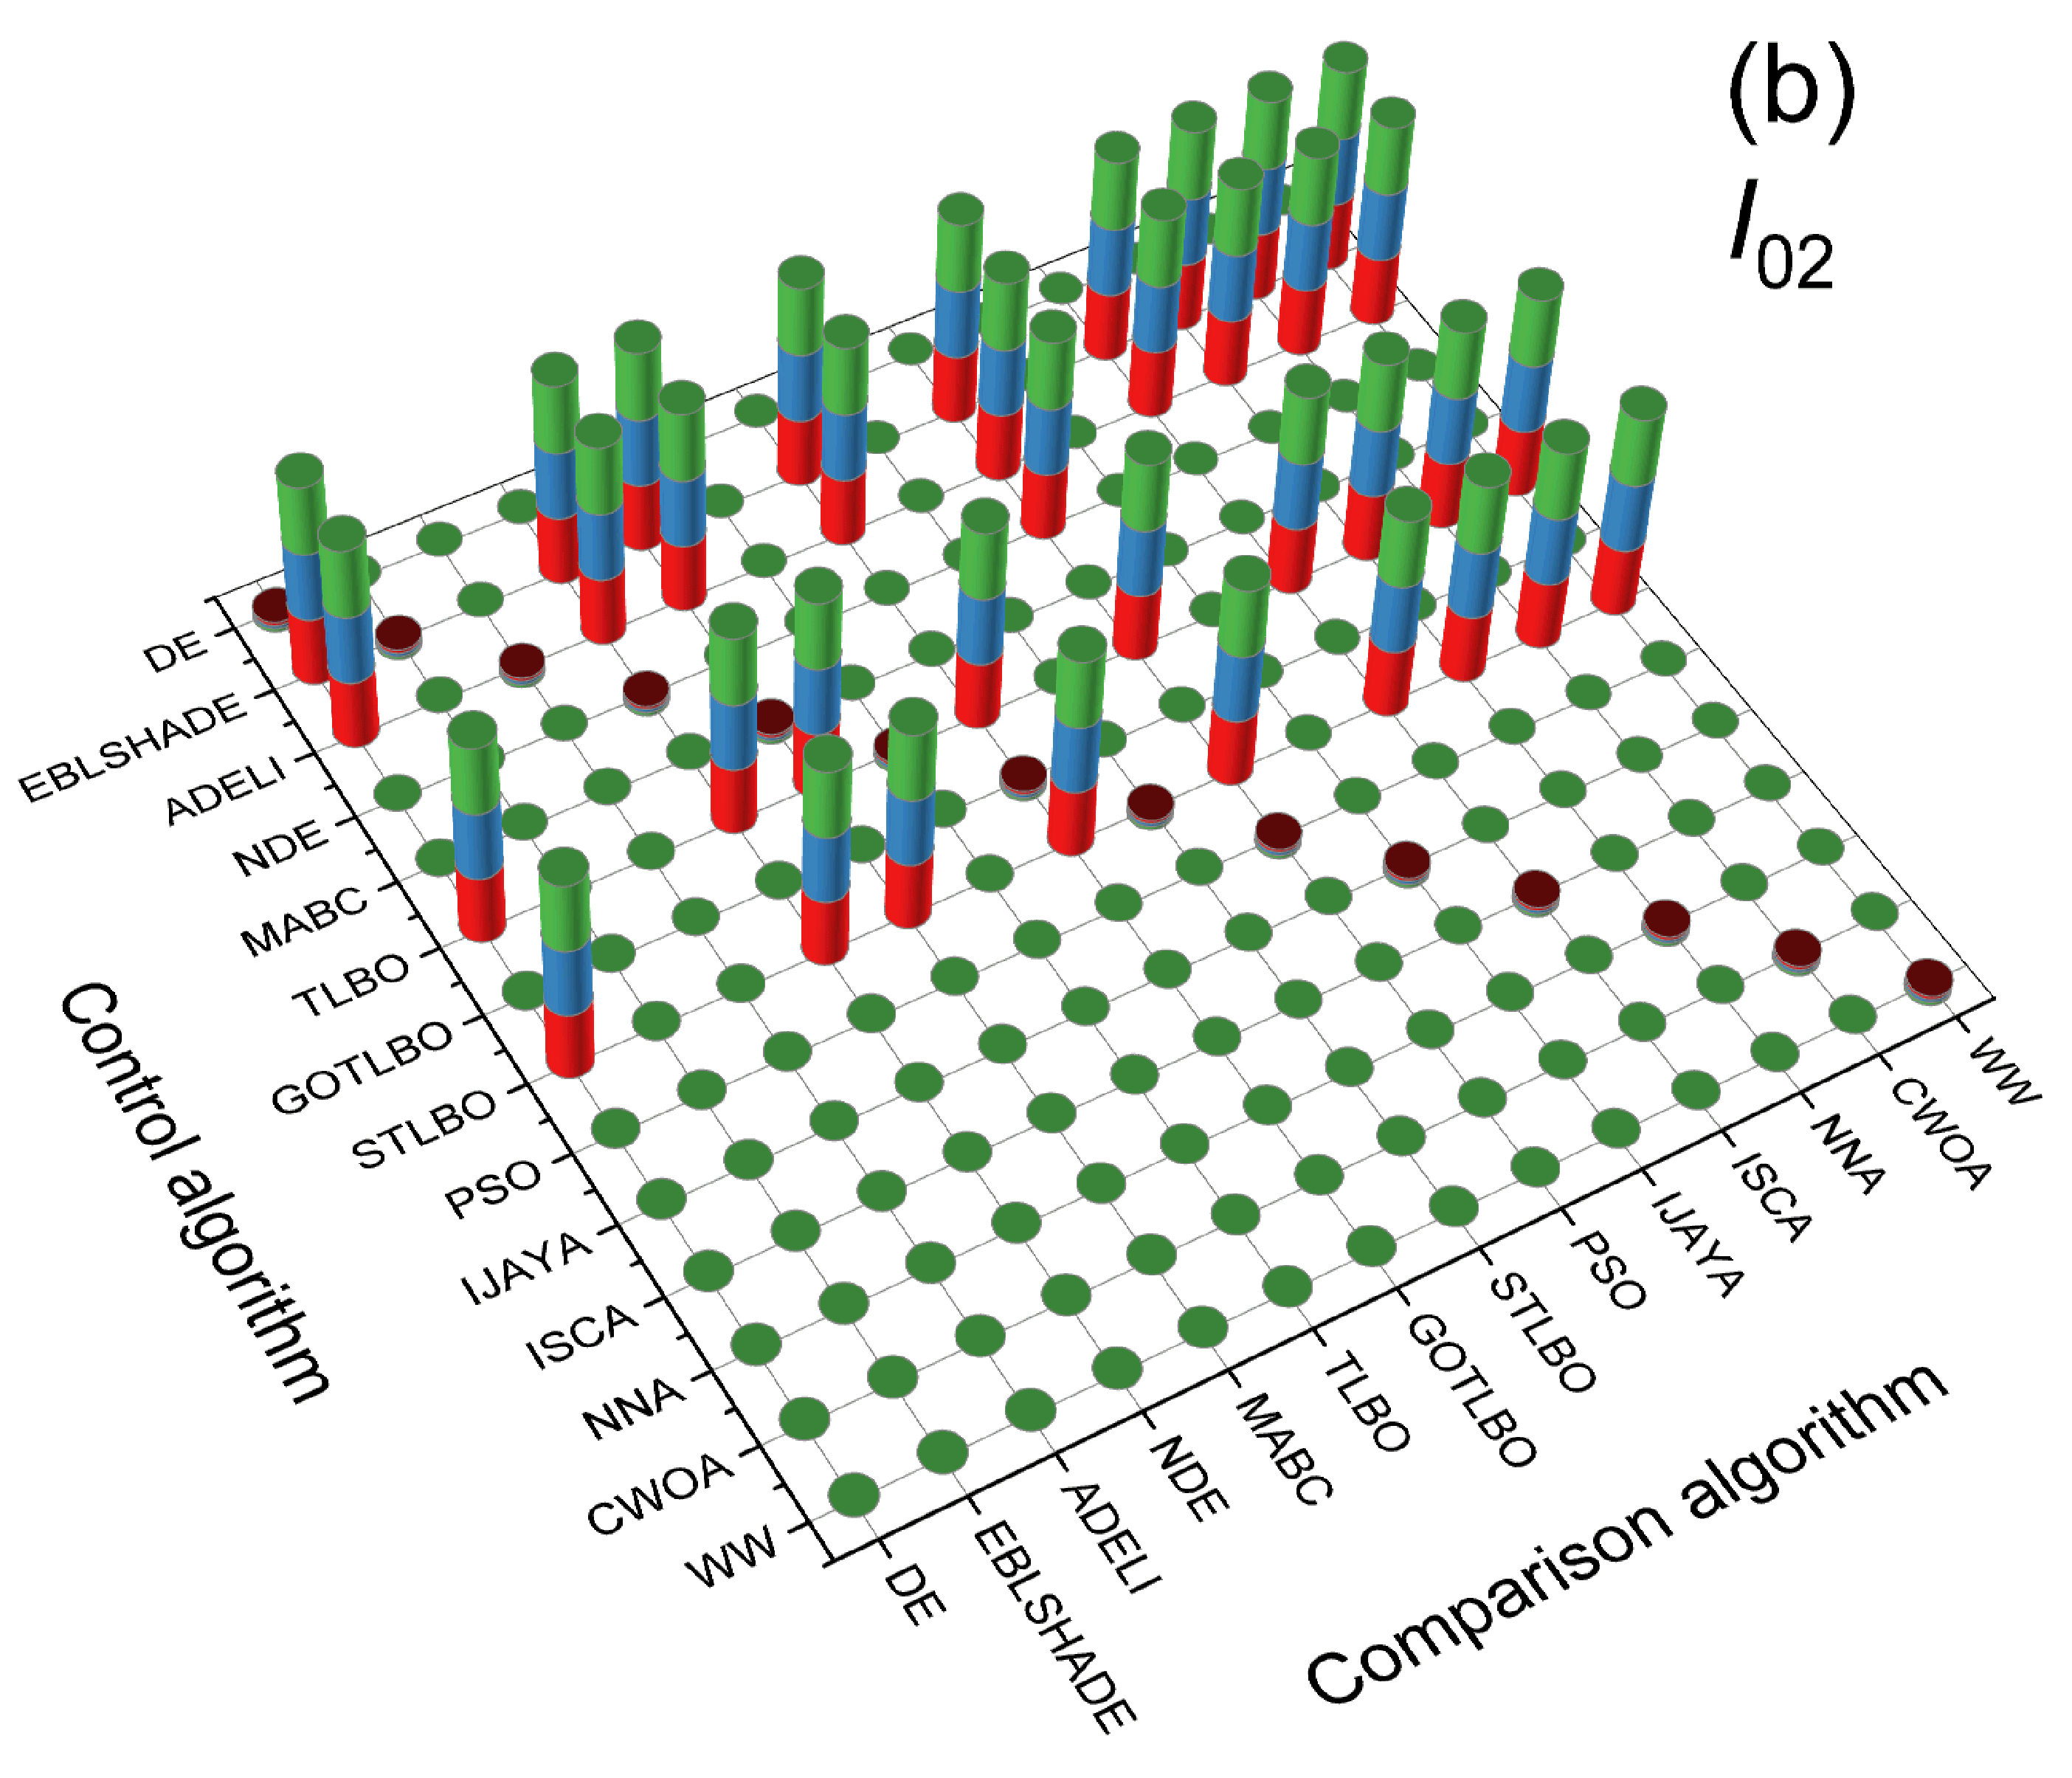
\includegraphics[width=.49\textwidth]{I02shot_NN}
	  \caption{The results of $N\times N$ multiple comparisons of $R_\mathrm{p1}$ (a) and $I_{02}$ (b) estimation
               among all algorithms in the single--IV case.
               The colored cylinder indicates that the adjusted $p$-value,
               which tests the control algorithm outperforms the comparison algorithm,
               is not greater than $p_{lim}=0.1$.
               The correspondence between the color of the cylinder to a post-hoc procedure is shown in the figure's legend.
               }\label{figNNRezSingleIV}
\end{figure*}

\begin{table*}[<options>]
\caption{The total count of wins and losses for each algorithm in $N\times N$ multiple comparisons using the
Friedman test and Shaffer's static, Nemenyi, and Holm post-hoc procedures
in single--IV case.
The criterion for victory was a adjusted $p$-value less than 0.1.
}\label{tblNNWins}
\begin{tabular*}{\tblwidth}{@{}LCCCCCCCCCCC@{}}
\toprule
\multirow{3}{*}{Algorithm}& \multicolumn{11}{C}{Wins / Loses} \\
&  \multicolumn{10}{C}{task}  &\multirow{2}{*}{Total}\\
  & $I_{01}$& $n_1$ & $R_\mathrm{p1}$ &$I_{02}$& $n_2$& $R_\mathrm{p2}$&$R_\mathrm{s}$&$I_\mathrm{ph}$&RMSPE&Comp&\\ % Table header row
\midrule
DE & 0/12 & 17/12 & 17/12 &  0/12 & 12/12 & 14/12 & 5/12  & 17/12  & 15/15 & 0/0  & 97/111\\
EBLSHADE & 27/0 & 27/0  & 27/0  & 27/0  & 27/0  & 27/0  & 27/0 & 27/0  &  26/0& 21/0  & \textbf{263}/\textbf{0} \\
ADELI & 27/0 & 27/0  &  27/0 &  27/0 &  27/0 &  27/0 & 27/0  & 27/0  &  27/0& 14/0  & 257/\textbf{0}\\
NDE & 0/12  & 21/12  & 18/11  & 3/12  & 18/9  & 3/12  &  18/11 & 21/9 & 24/8 & 0/0  & 126/96\\
MABC &  0/12& 0/15& 10/12  &  0/12 & 11/12  & 0/17  & 3/12  & 2/15  & 12/15 & 0/3  & 38/125\\
TLBO & 27/0& 27/0 & 26/0 &  27/0&  24/0& 27/0 & 26/0 & 24/0 & 24/0 & 10/0  & 242/0\\
GOTLBO & 0/12  & 0/18  & 0/24  & 0/12  & 3/15  & 0/12 & 3/15  & 0/21 & 0/21  & 0/5  & 6/155\\
STLBO & 27/0 & 27/0  & 27/0  & 27/0  & 27/0  & 27/0  & 27/0  & 27/0  & 27/0 & 11/0  & 254/\textbf{0}\\
PSO & 0/12  & 0/21  & 0/24  & 0/15  & 0/24  & 0/21  &  0/34 & 0/23  & 0/18  & 0/12  & 0/204\\
IJAYA &  0/0 &  16/0 &  18/0 & 0/0  & 12/0 &  11/0 &  3/0 & 18/0  & 18/0  & 0/0  & 96/\textbf{0}\\
ISCA & 0/12  & 0/21  & 0/23  & 0/12  & 3/15  & 0/12  & 2/15  & 0/21  & 0/24 & 0/3  & 5/158\\
NNA & 3/12  & 0/21  & 0/23  & 0/12  & 0/23  & 0/14  & 0/17  & 0/21  & 0/24& 0/9  & 3/176\\
CWOA & 0/12  & 0/21  &  0/21& 0/12  & 0/24& 0/18  & 3/15  & 0/21  & 0/24 & 0/12  & 3/180\\
WW & 0/15  & 0/21  & 0/20&  0/12 & 0/30 & 0/18 & 2/15  & 0/20  & 0/24& 0/12  & 2/187\\
\bottomrule
\end{tabular*}
\end{table*}

In most instances, all post-hoc procedures considered lead to similar conclusions 
regarding the outperformance of one algorithm over another. 
For example, in the case of the $R_\mathrm{p1}$ estimation task, 
the Nemenyi procedure disagrees with the Holm and Shaffer methods in only 4 out of 57 cases.
Particularly, this happens for the hypotheses "DE vs WW," "MABC vs ISCA," "MABC vs NNA," and "TLBO vs NDE" --- see Fig.~\ref{figNNRezSingleIV}(a).
On the other hand, as evident from Fig.~\ref{figNNRezSingleIV}(b), 
such situations are not observed at all for the $I_{02}$ evaluation task.
In general, the results of the Holm procedure differ from those of the Shaffer procedure in only two comparisons: 
the improvement of IJAYA over GOTLBO in the $n_1$  estimation and the outperformance of TLBO over NNA for the composite parameter.


Totally $1\times N$ multiple comparisons exhibit more powerful behavior than $N\times N$ ones, resulting in lower $p$-values.
As a result, IJAYA did not lose in any of the $N\times N$ comparisons --- see Table~\ref{tblNNWins}.
Another striking  example can be observed when considering the case of the composite parameter.
Based on the $1\times N$ comparisons, conclusions were drawn about the outperformance of one algorithm over another in 67 cases,
whereas for the $N\times N$ comparisons, such situations were identified in only 20 cases:
the improvement of EBLSHADE over MABC, GOTLBO, PSO, ISCA, NNA, CWOA, and WW,
the statistically significant difference ADELI and GOTLBO, PSO, NNA, CWOA, and WW,
and outperformance of both TLBO and STLBO over PSO, NNA, CWOA, and WW.
As a result, $N\times N$ comparisons yield a less precise ranking of all algorithms. 
Nonetheless, it remains feasible to discern the best and worst-performing algorithms. 
The data obtained reveal that EBLSHADE, ADELI, and STLBO consistently emerge as the top-performing algorithms across all tasks, 
while PSO, ISCA, NNA, CWOA, and WW consistently rank among the worst performers.

Thus, the results presented in this subsection demonstrate that 
no examined algorithm can be defined as one that allows for precisely estimating only one 
(e.g., only $R_\mathrm{p2}$ or only $I_{02}$) parameter in the opposed two-diode model.
The algorithms that exhibit high efficiency (EBLSHADE, ADELI, and STLBO) 
allow for the most precise estimation of all parameters. 
However, certain algorithms indeed display higher accuracy in determining specific parameters.
Indeed, DE and IJAYA are the most effective in estimating $R_\mathrm{p2}$ and $I_\mathrm{ph}$, as shown in see table~S1.
Nevertheless, this highest level of accuracy appears not worth significant attention when compared to other optimization methods. 
As a result, the performance metrics of algorithms for individual parameter evaluation will not be analyzed in the following subsection, 
which is dedicated to the analysis of \emph{IV} curves with different parameter ratios.


%Будь-ласка, покращ англійську в наступних реченнях, які я буду пропонувати. Зокрема, треба буде виправити граматичні та стилістичні помилки
%якщо можна, окрім виправленого речення, наводь інформацію про зміни, які зроблені


\subsubsection{Parameter extraction in IV--set case}


\begin{figure*}[]
	\centering
		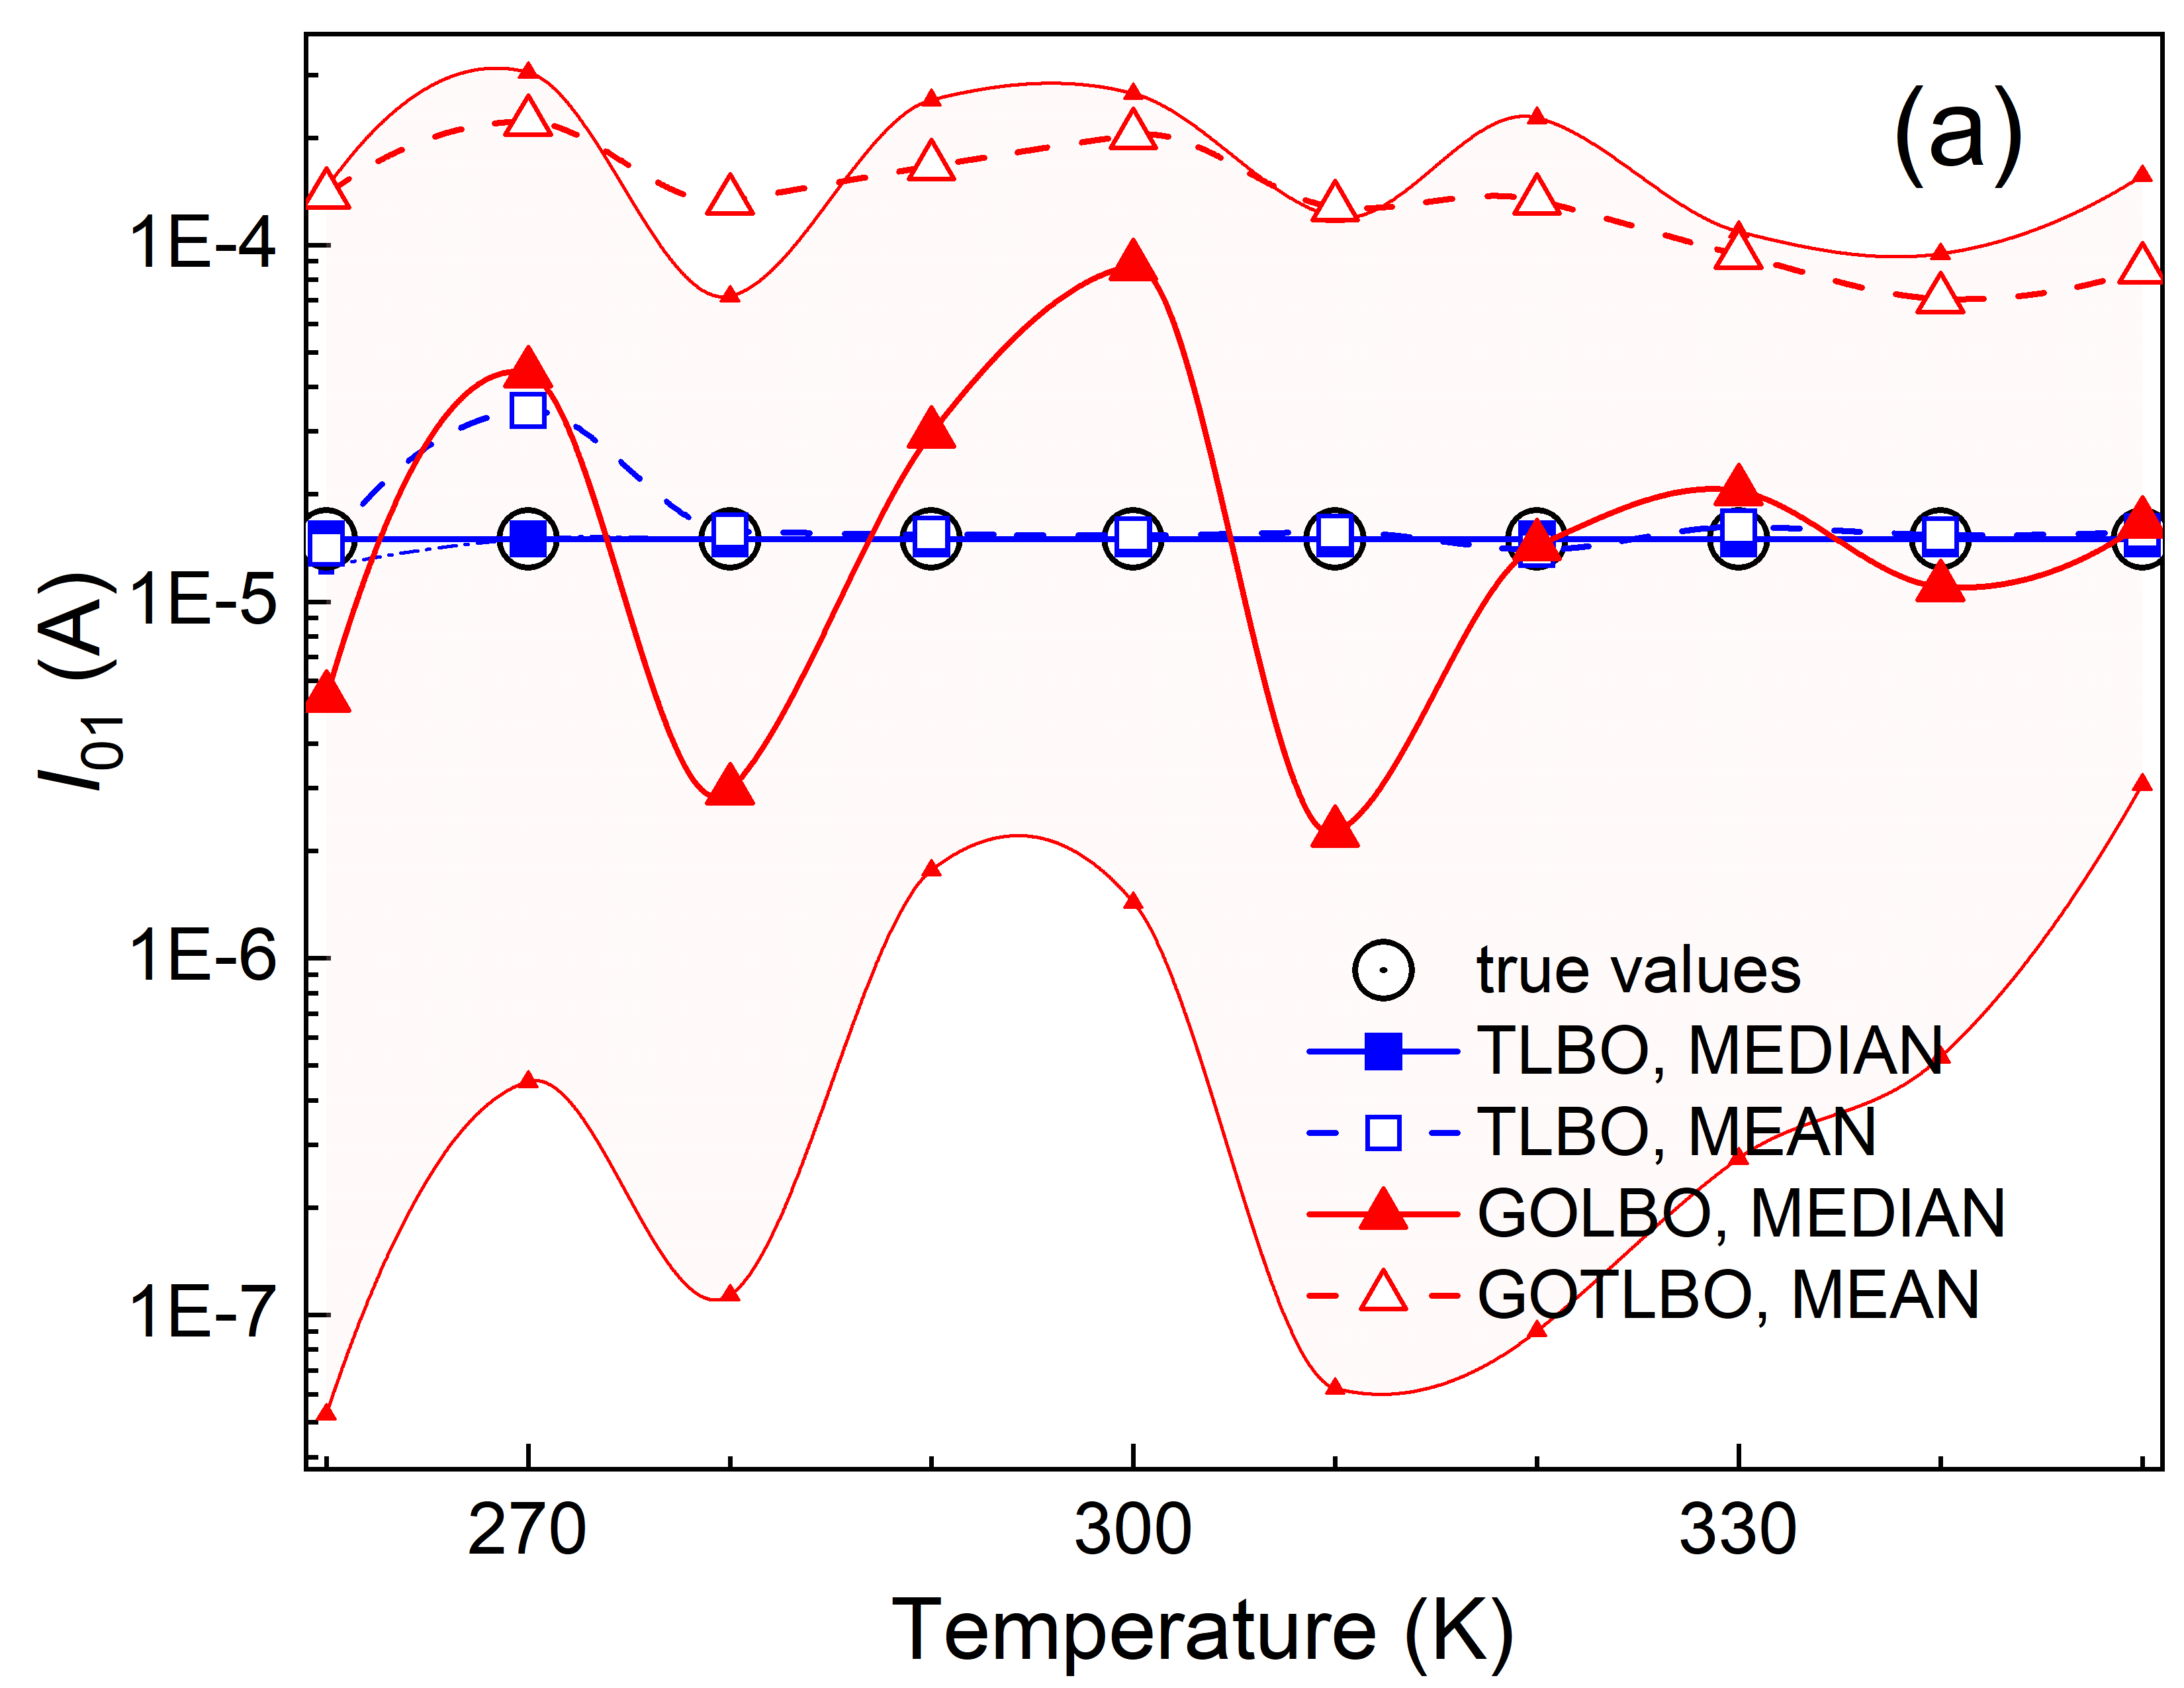
\includegraphics[width=.32\textwidth]{AfigA}
        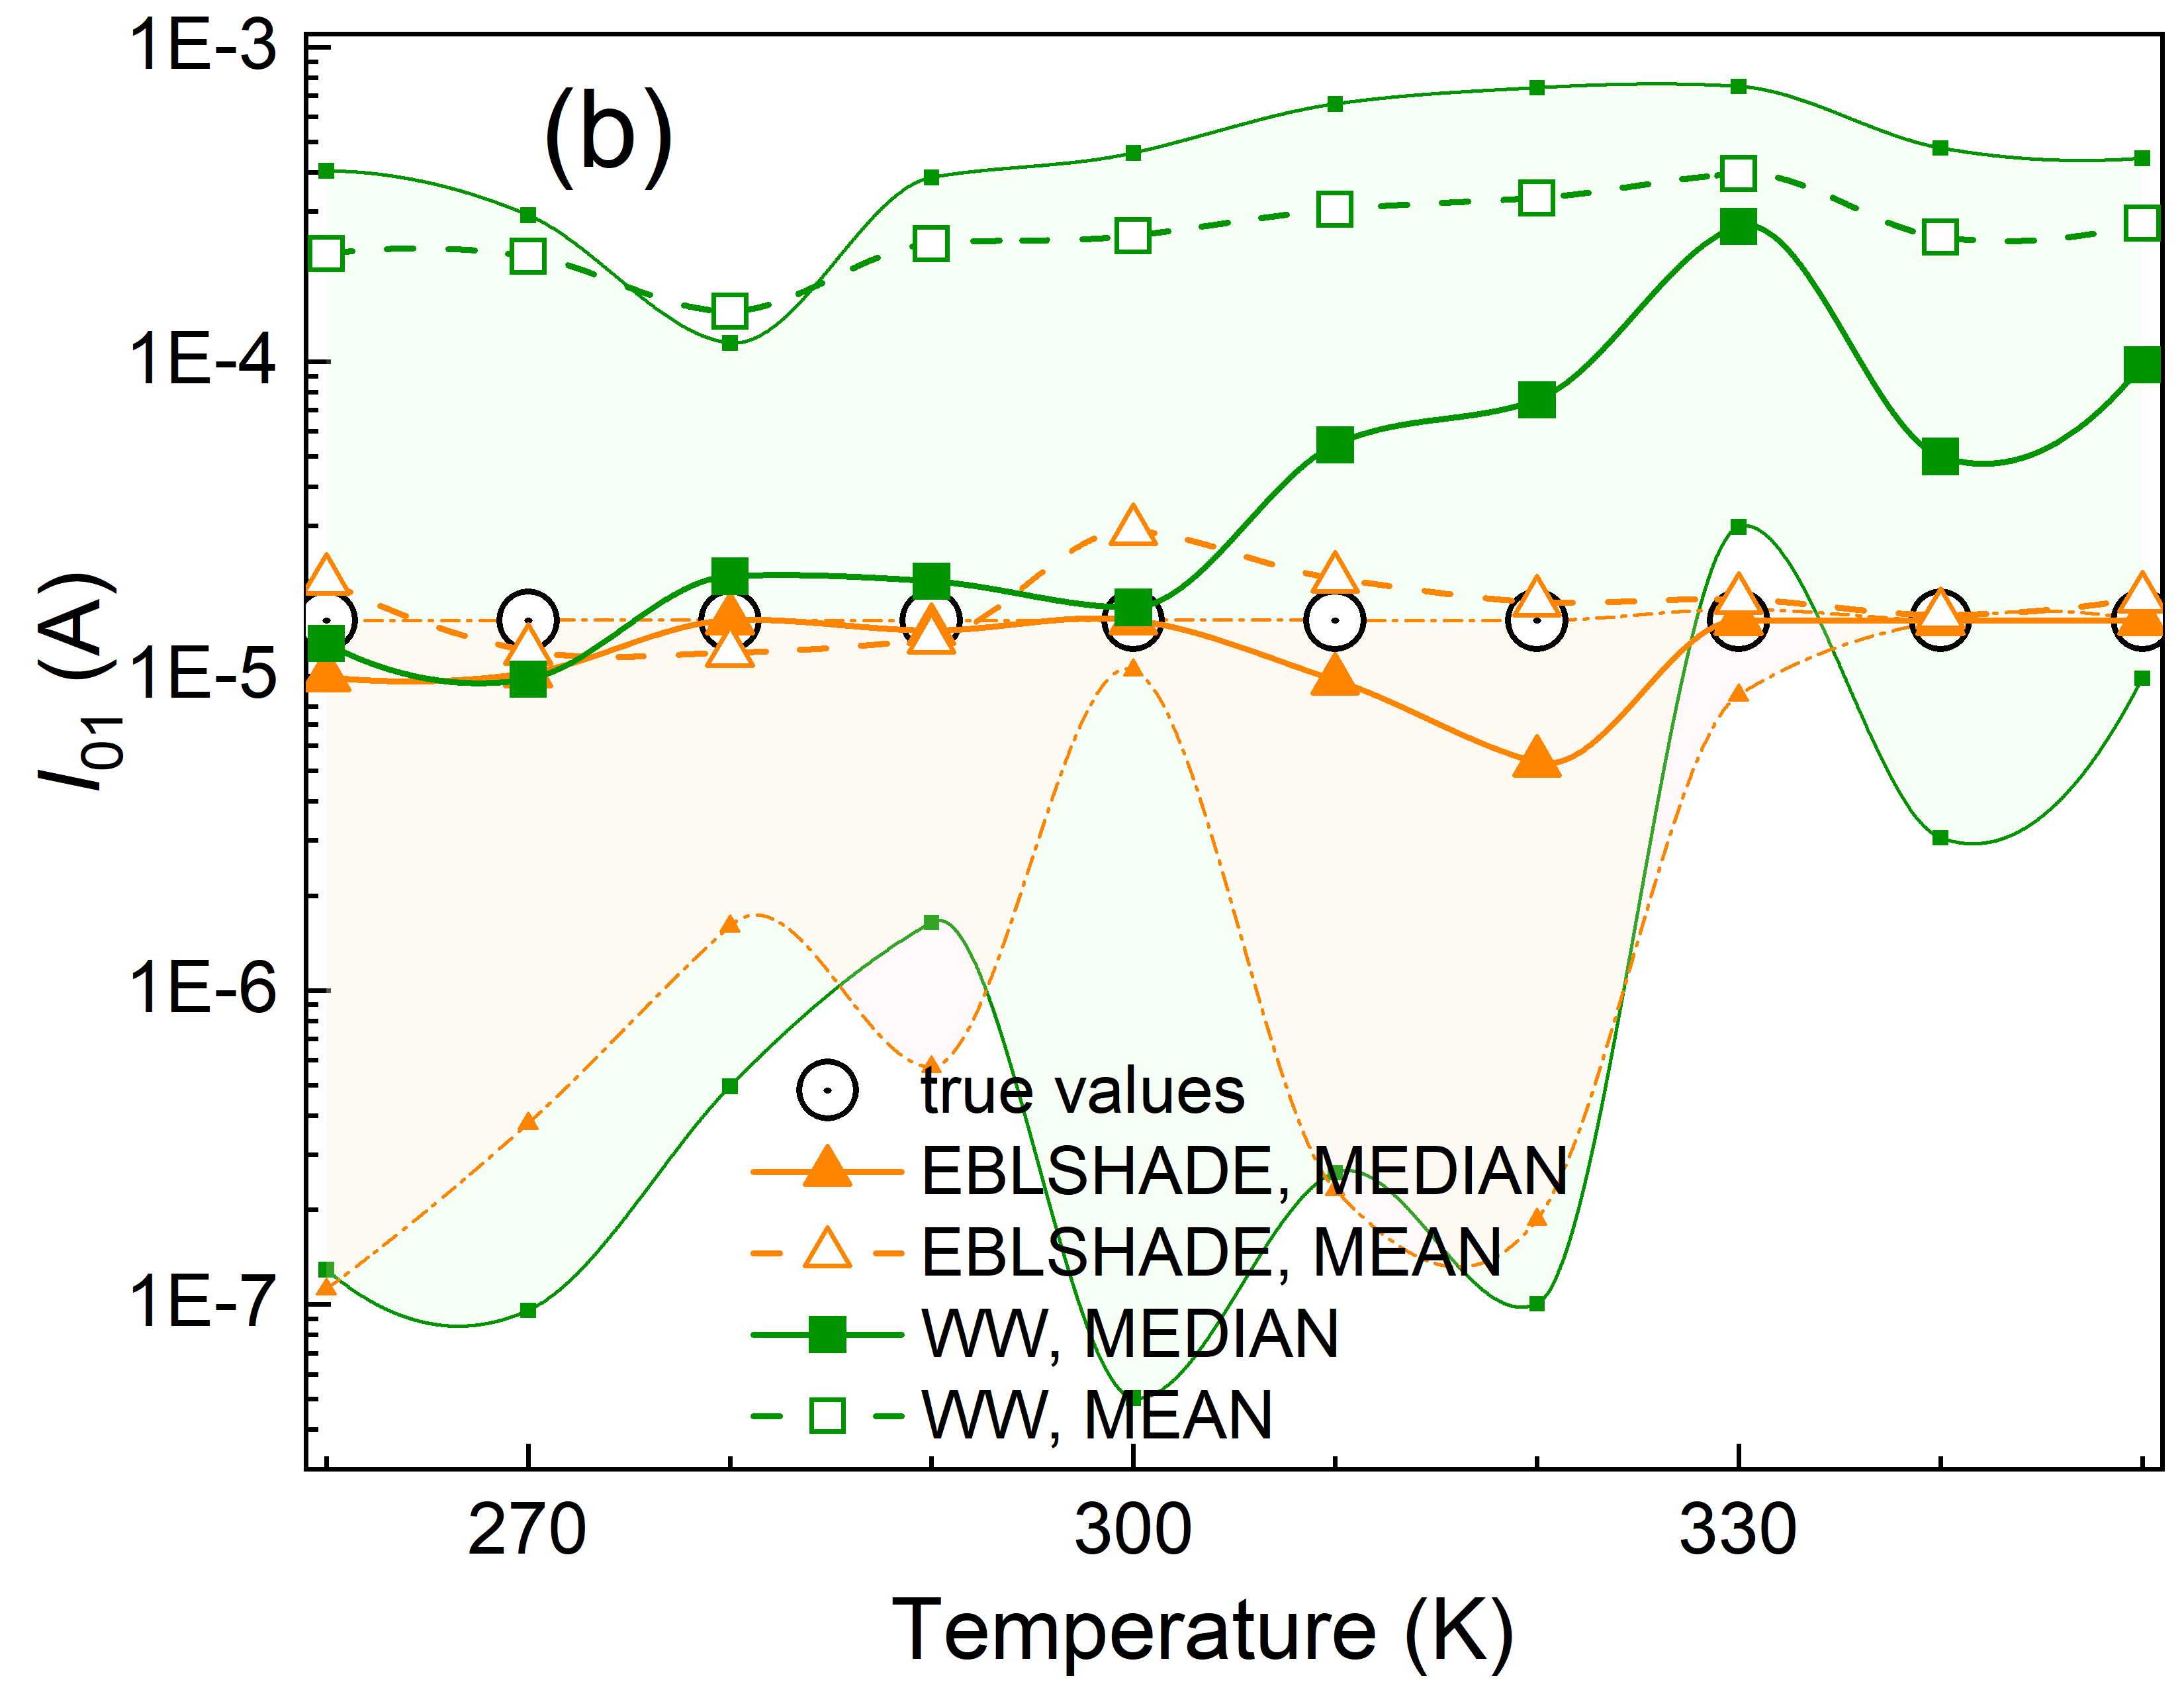
\includegraphics[width=.32\textwidth]{AfigB}
        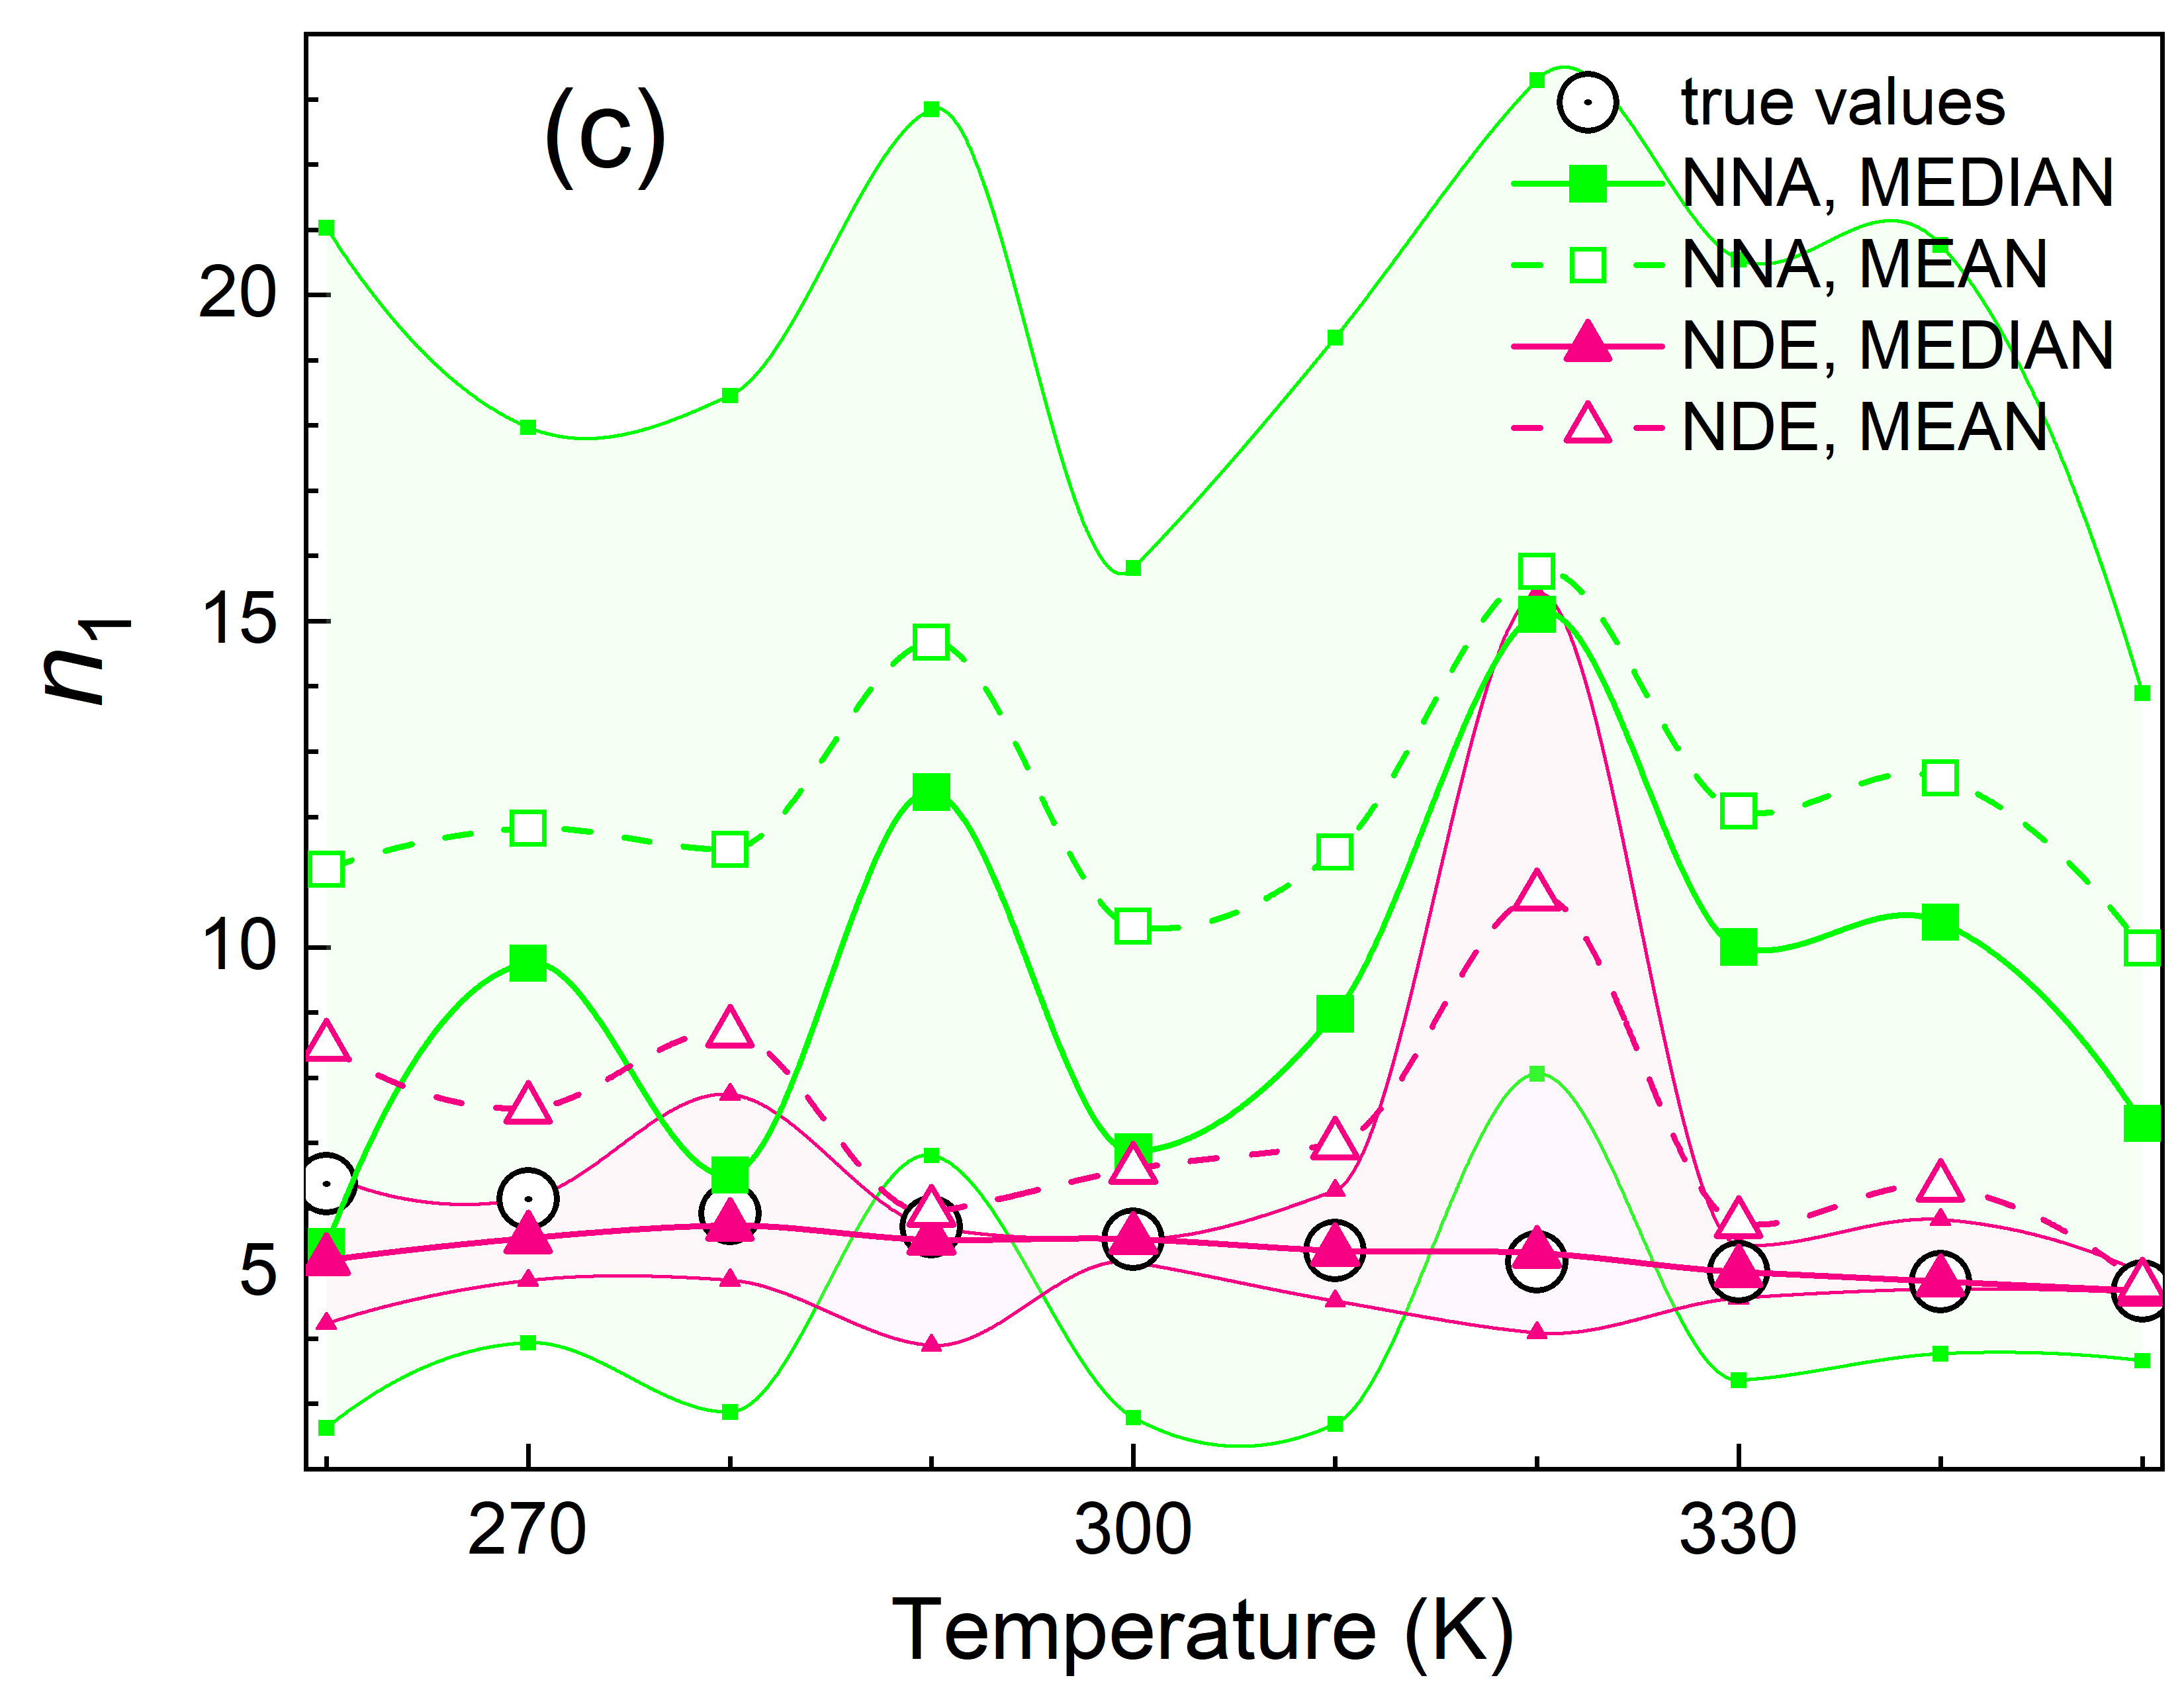
\includegraphics[width=.32\textwidth]{AfigC}
		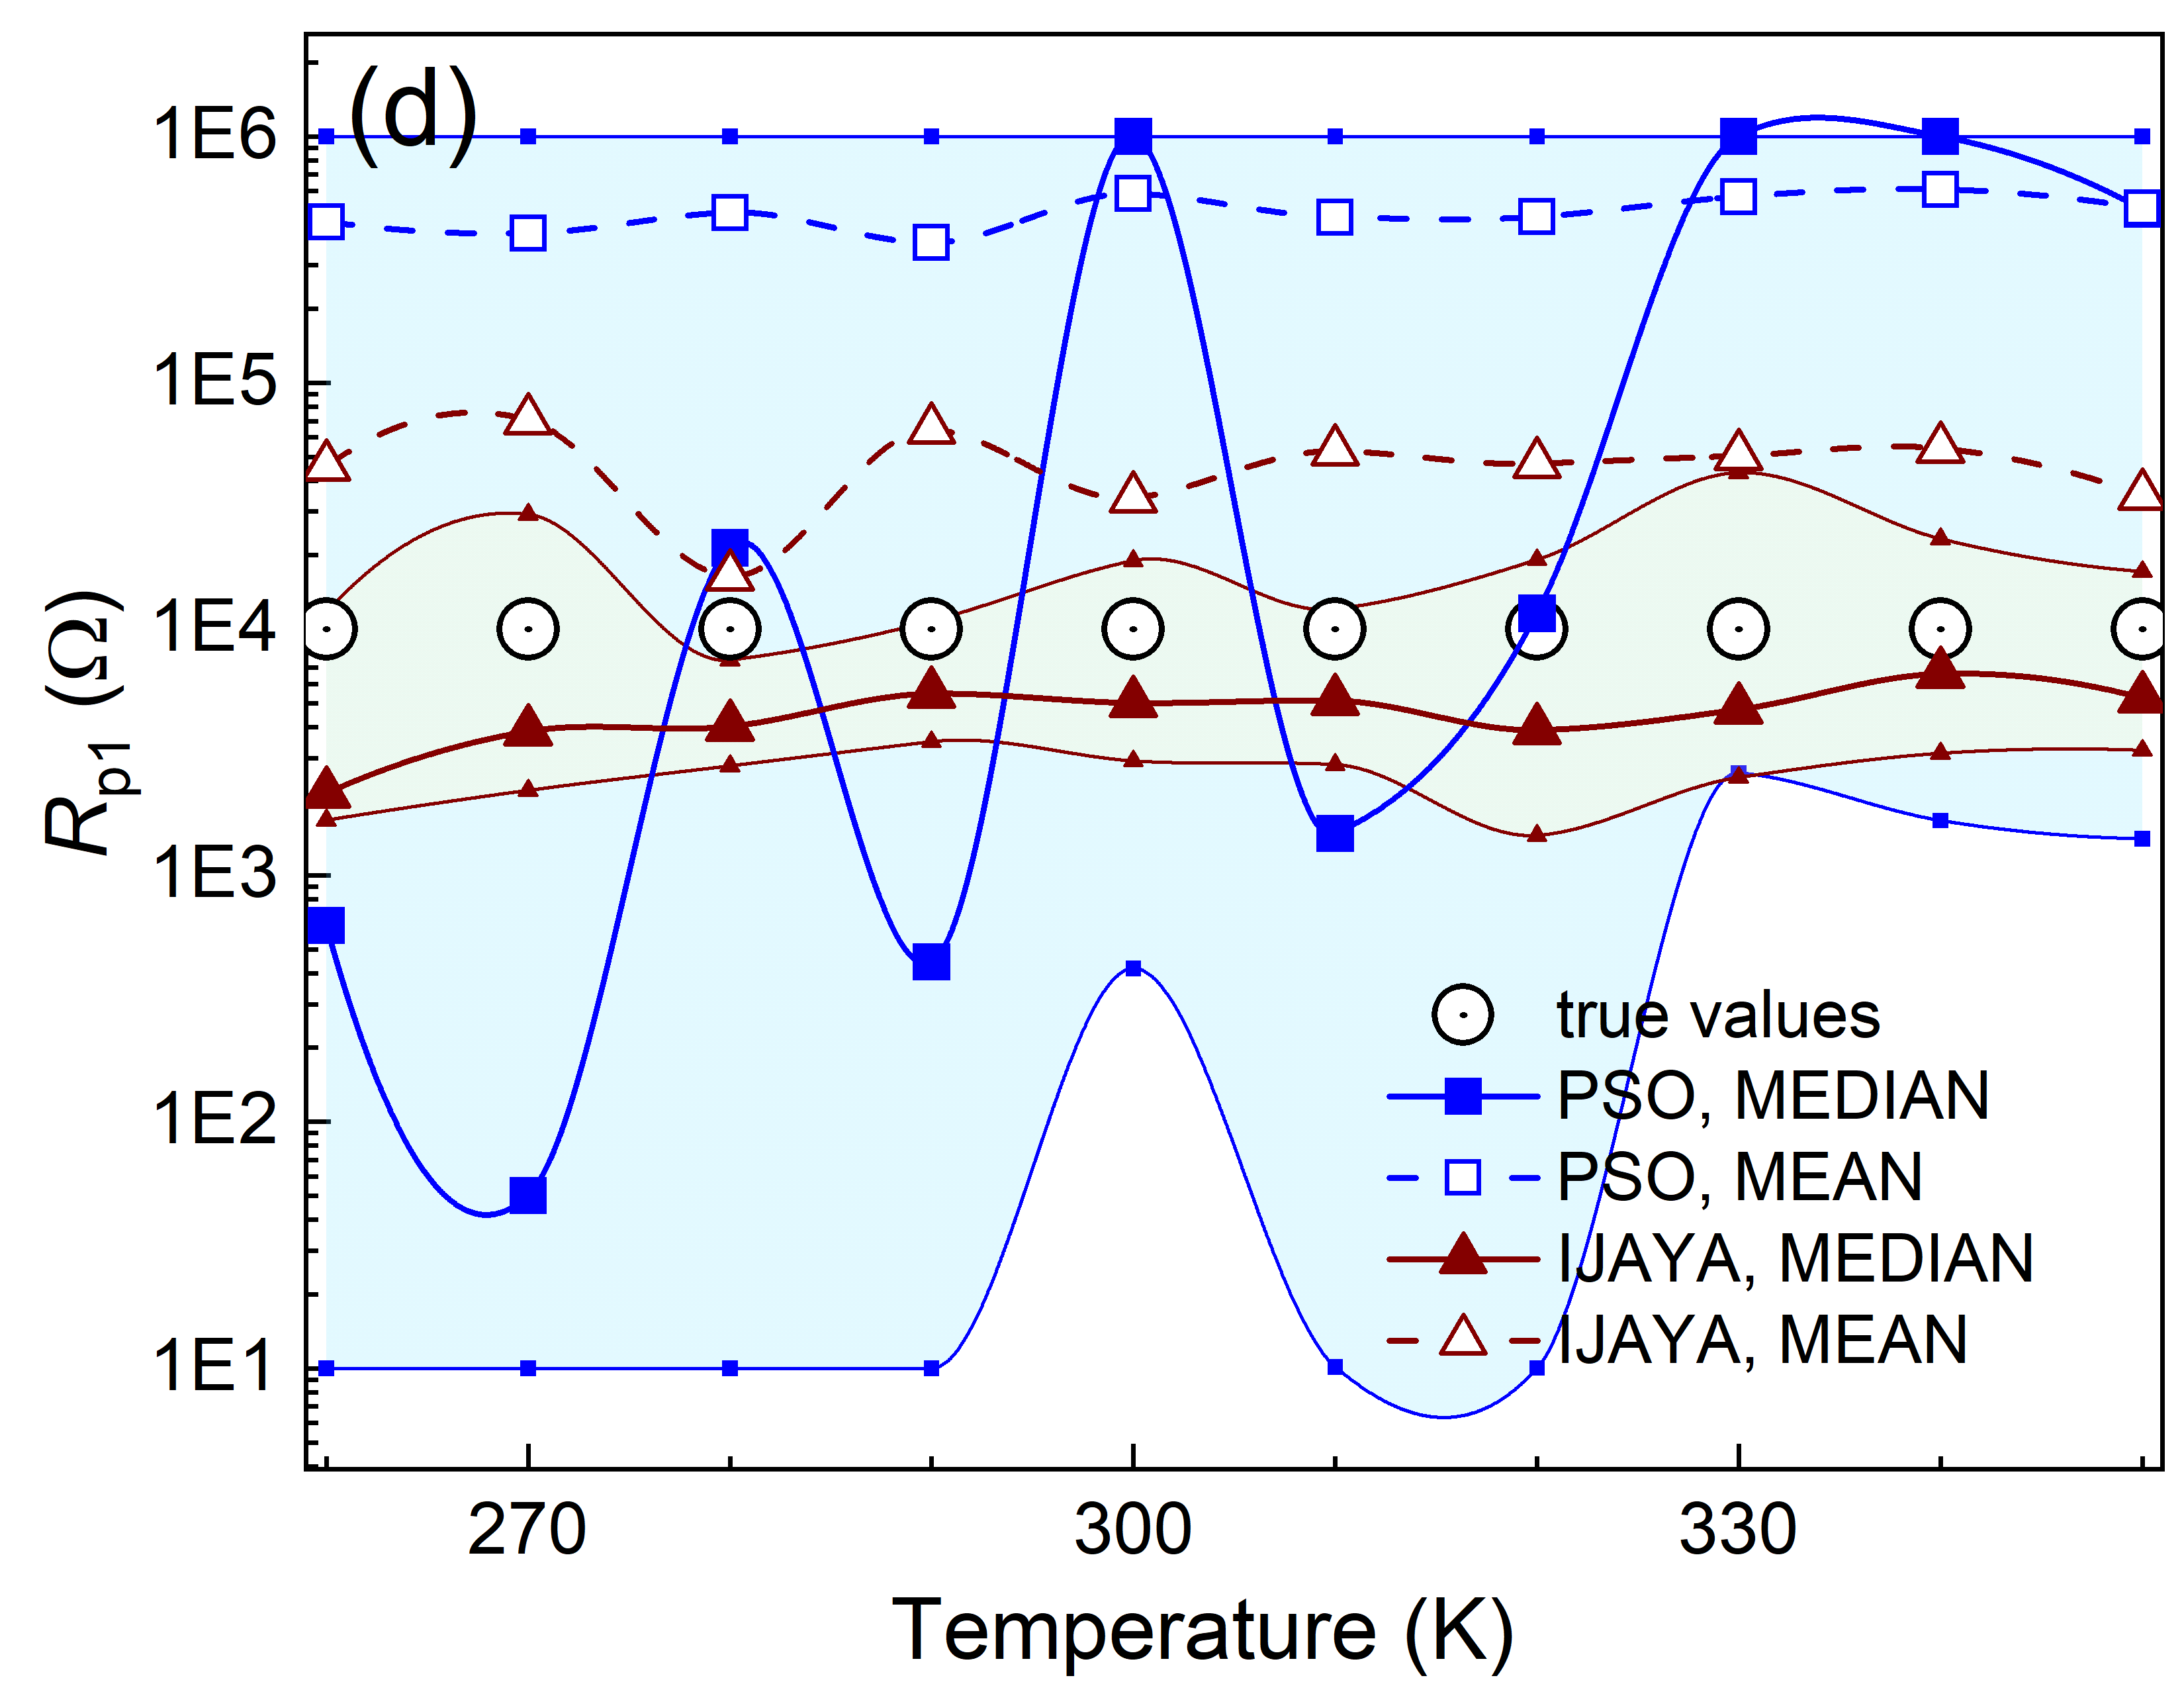
\includegraphics[width=.32\textwidth]{AfigD}
        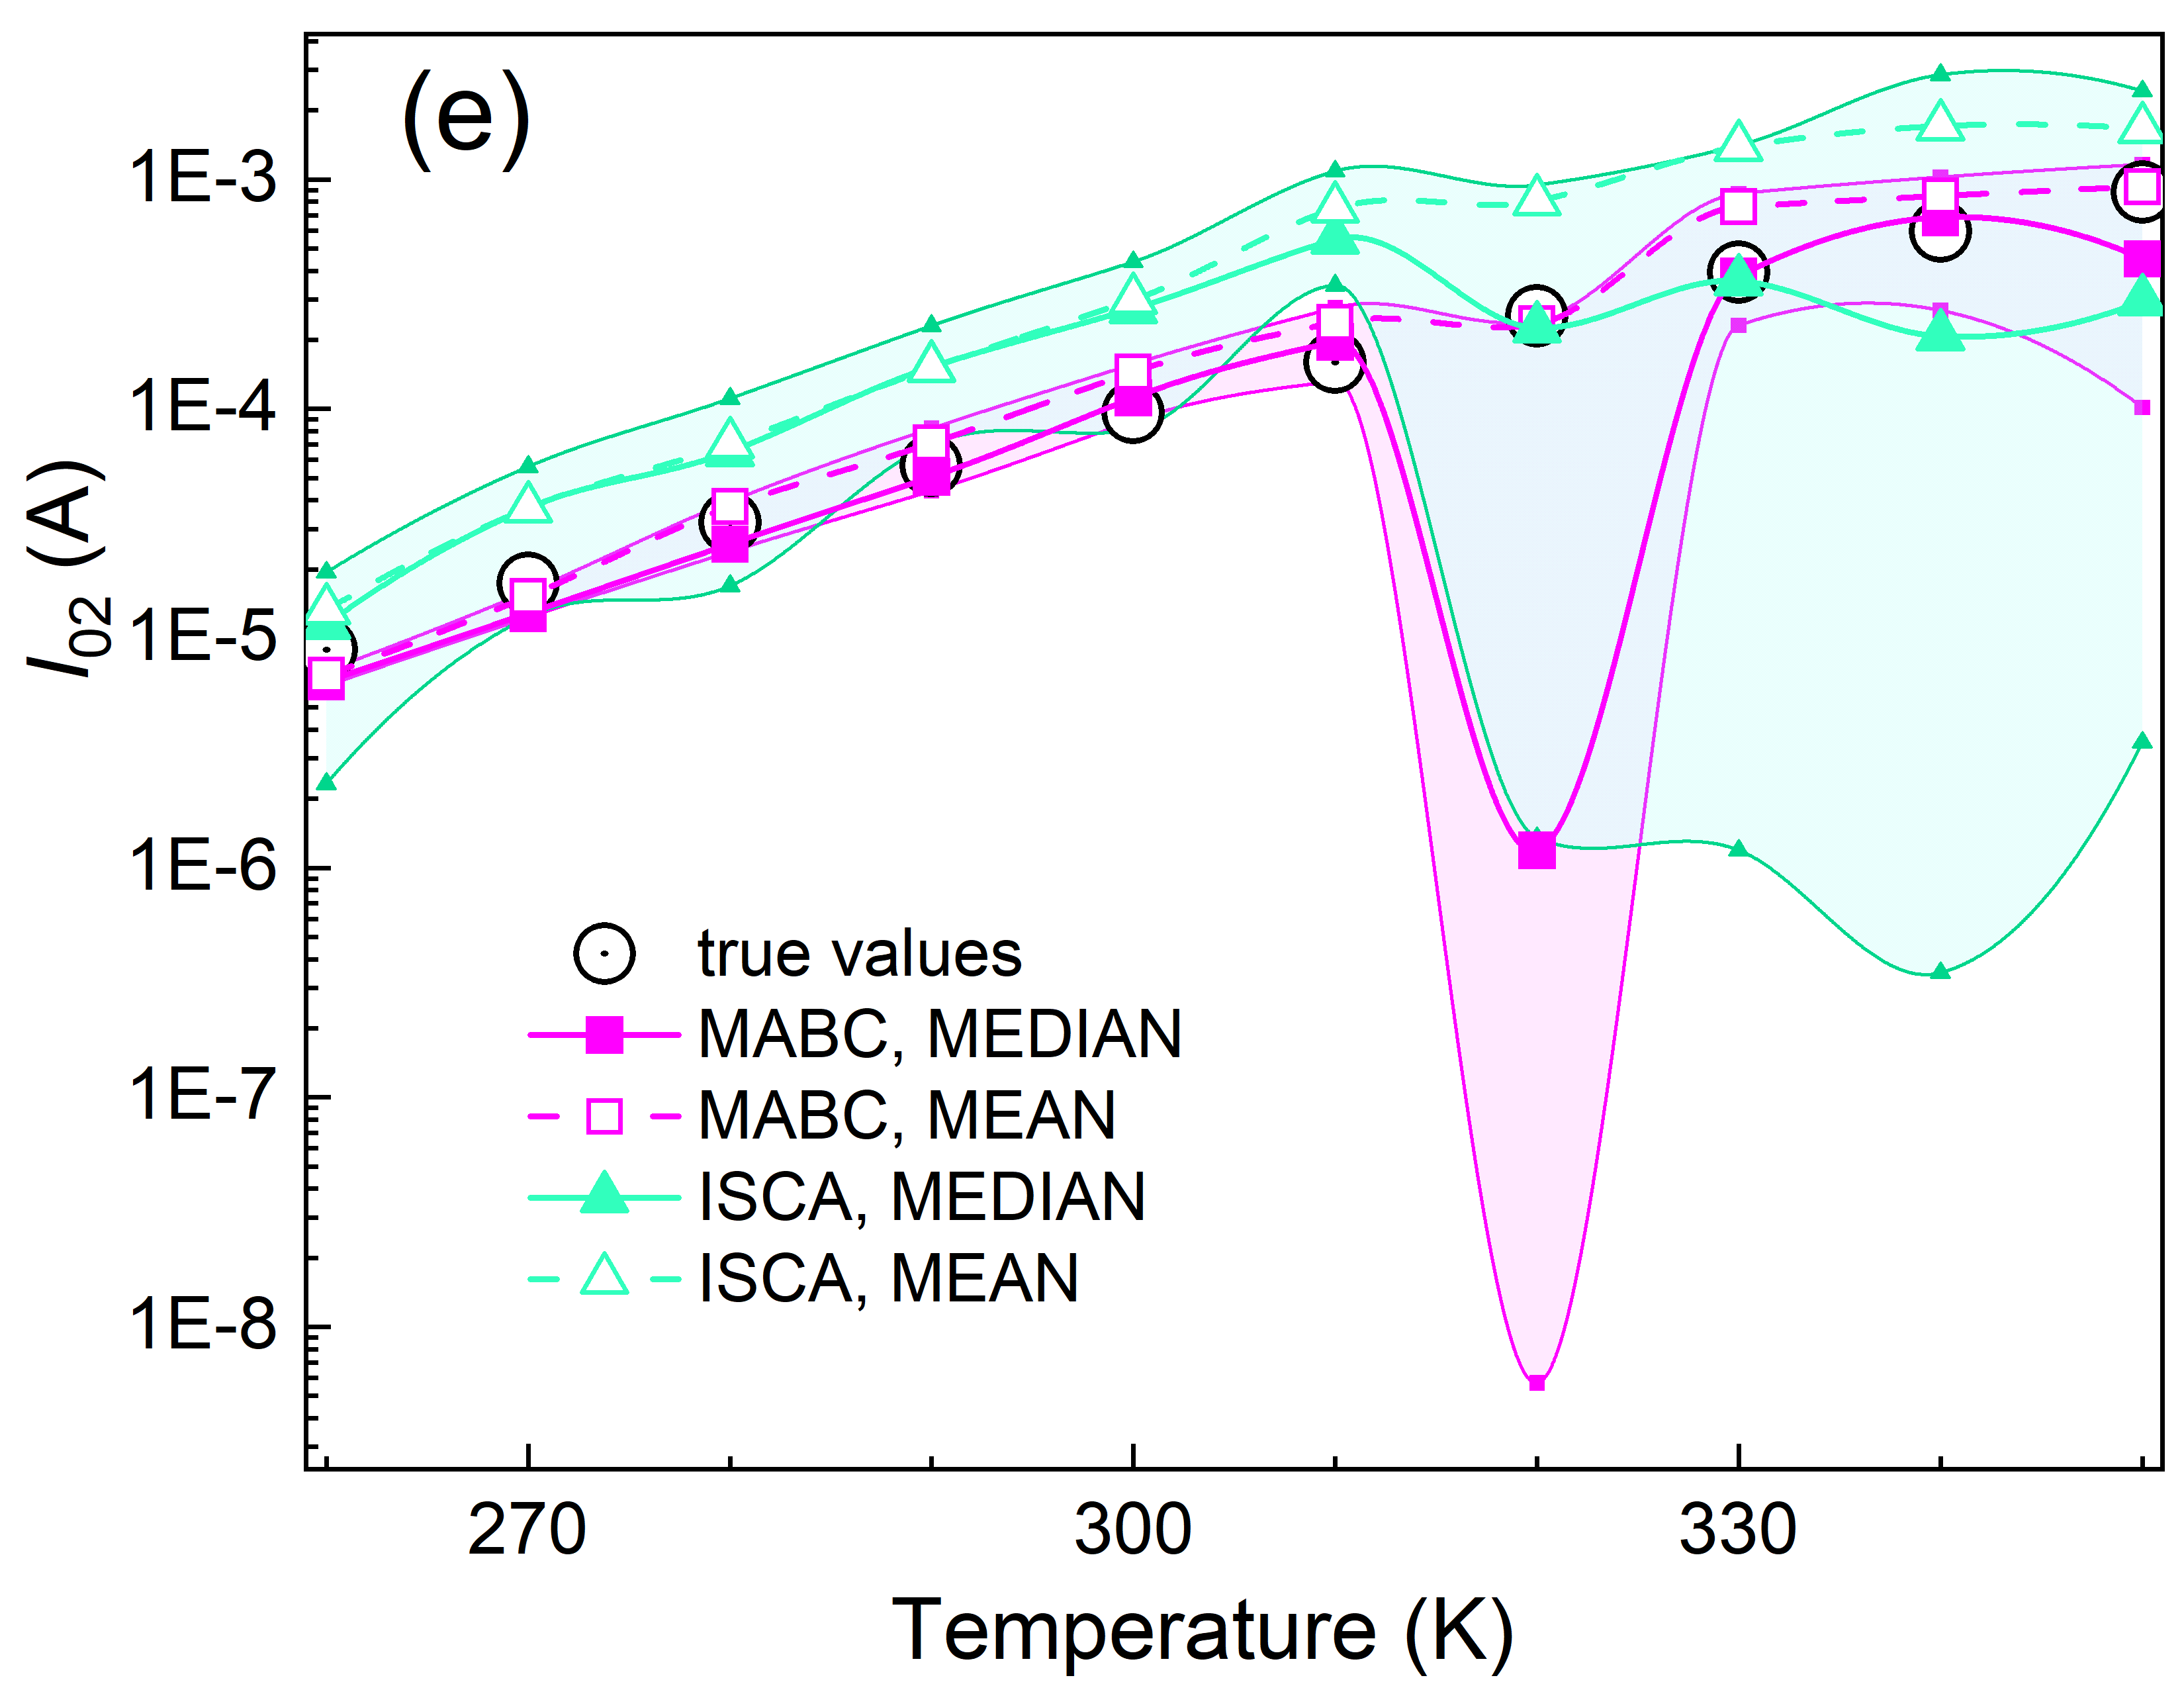
\includegraphics[width=.32\textwidth]{AfigE}
        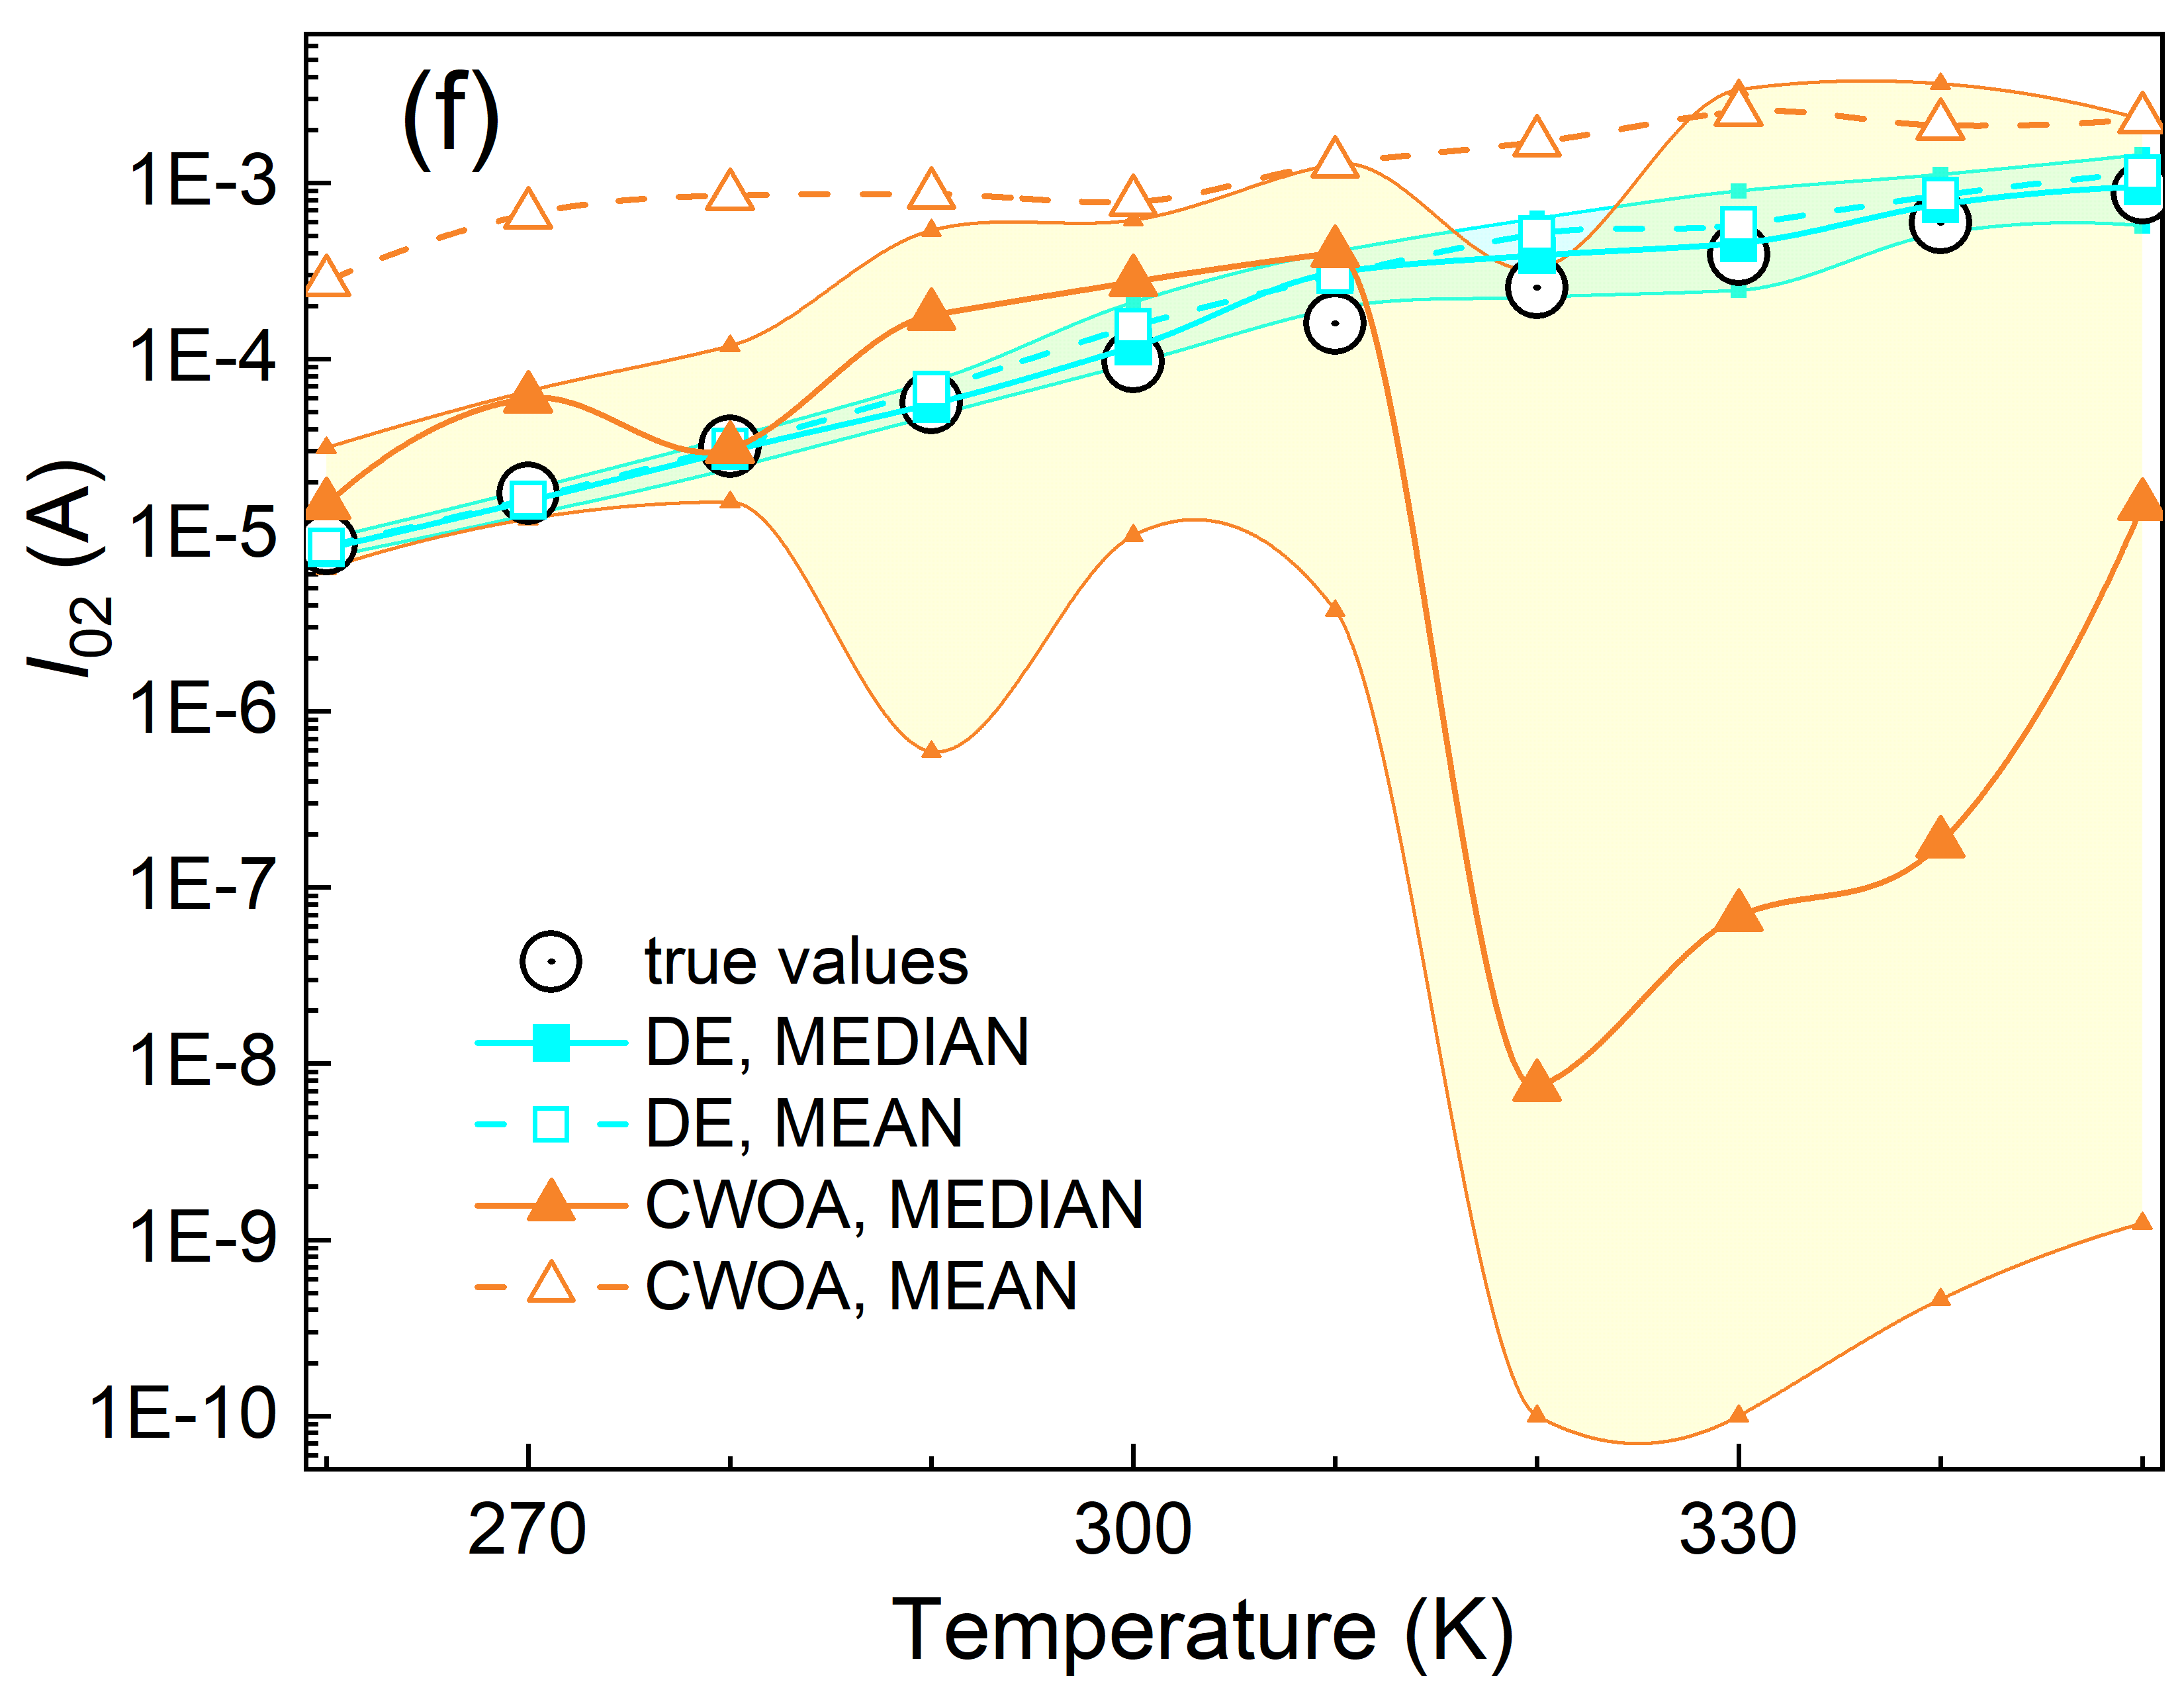
\includegraphics[width=.32\textwidth]{AfigF}
		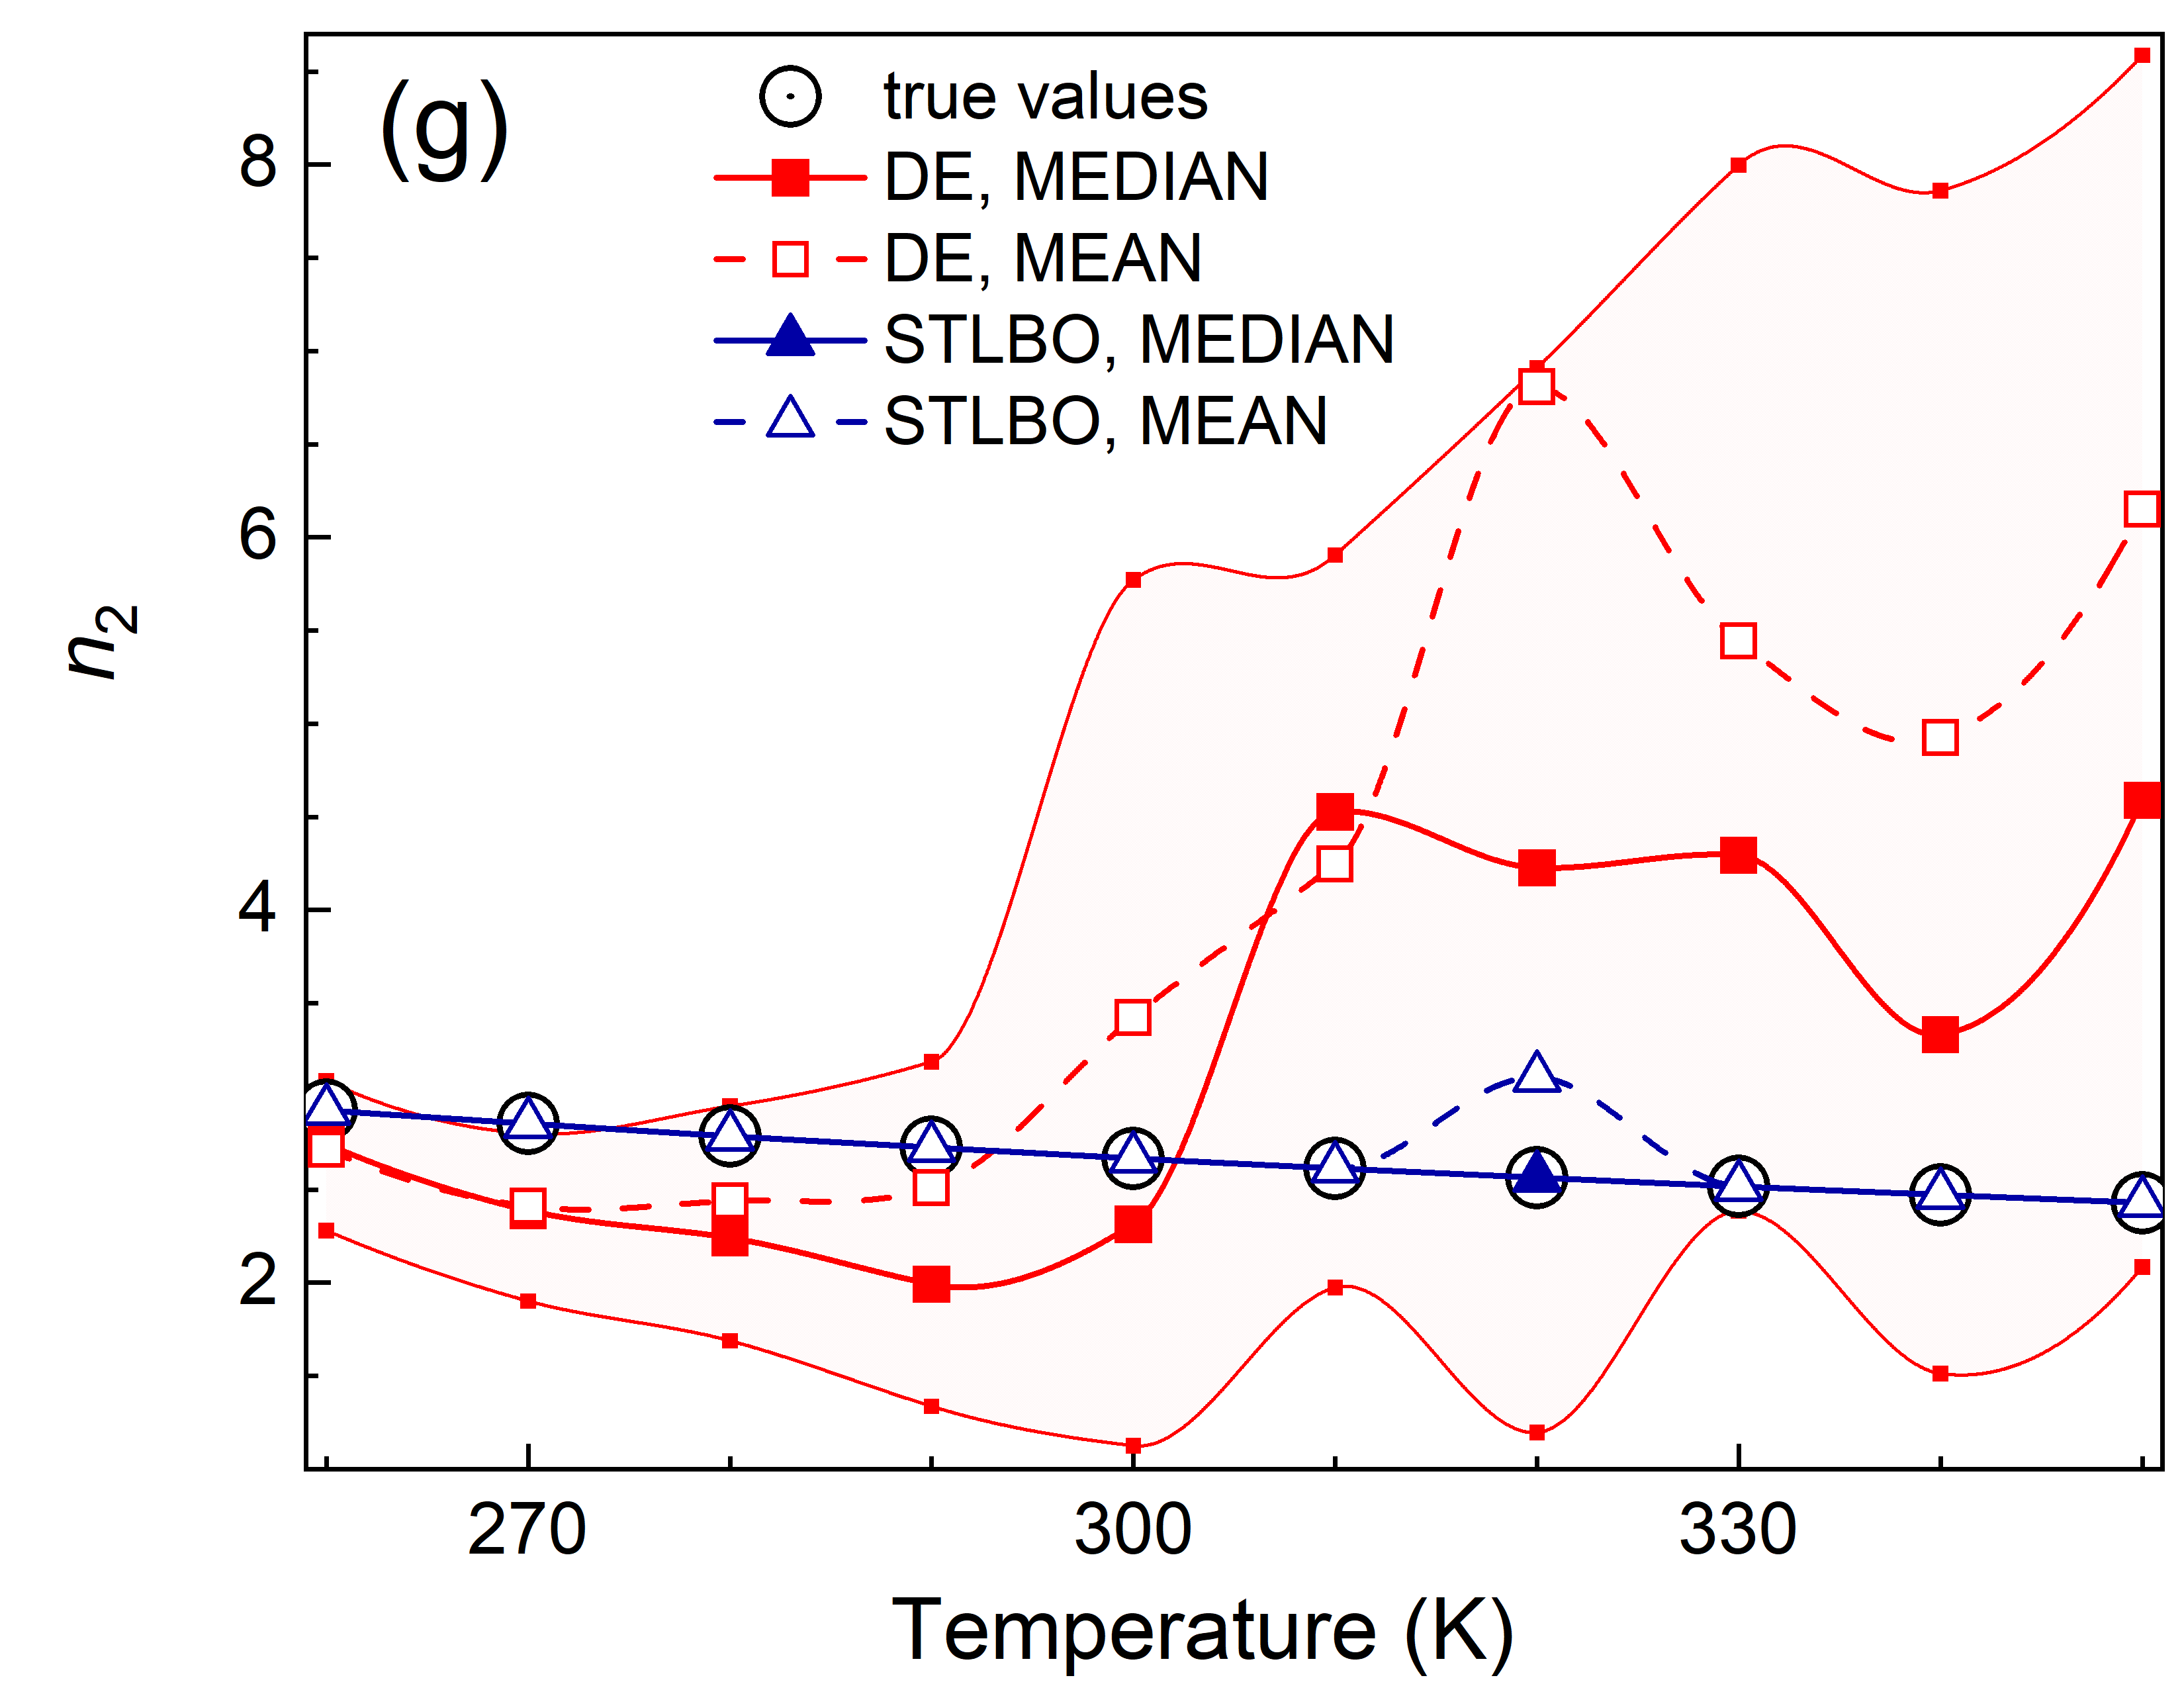
\includegraphics[width=.32\textwidth]{AfigG}
        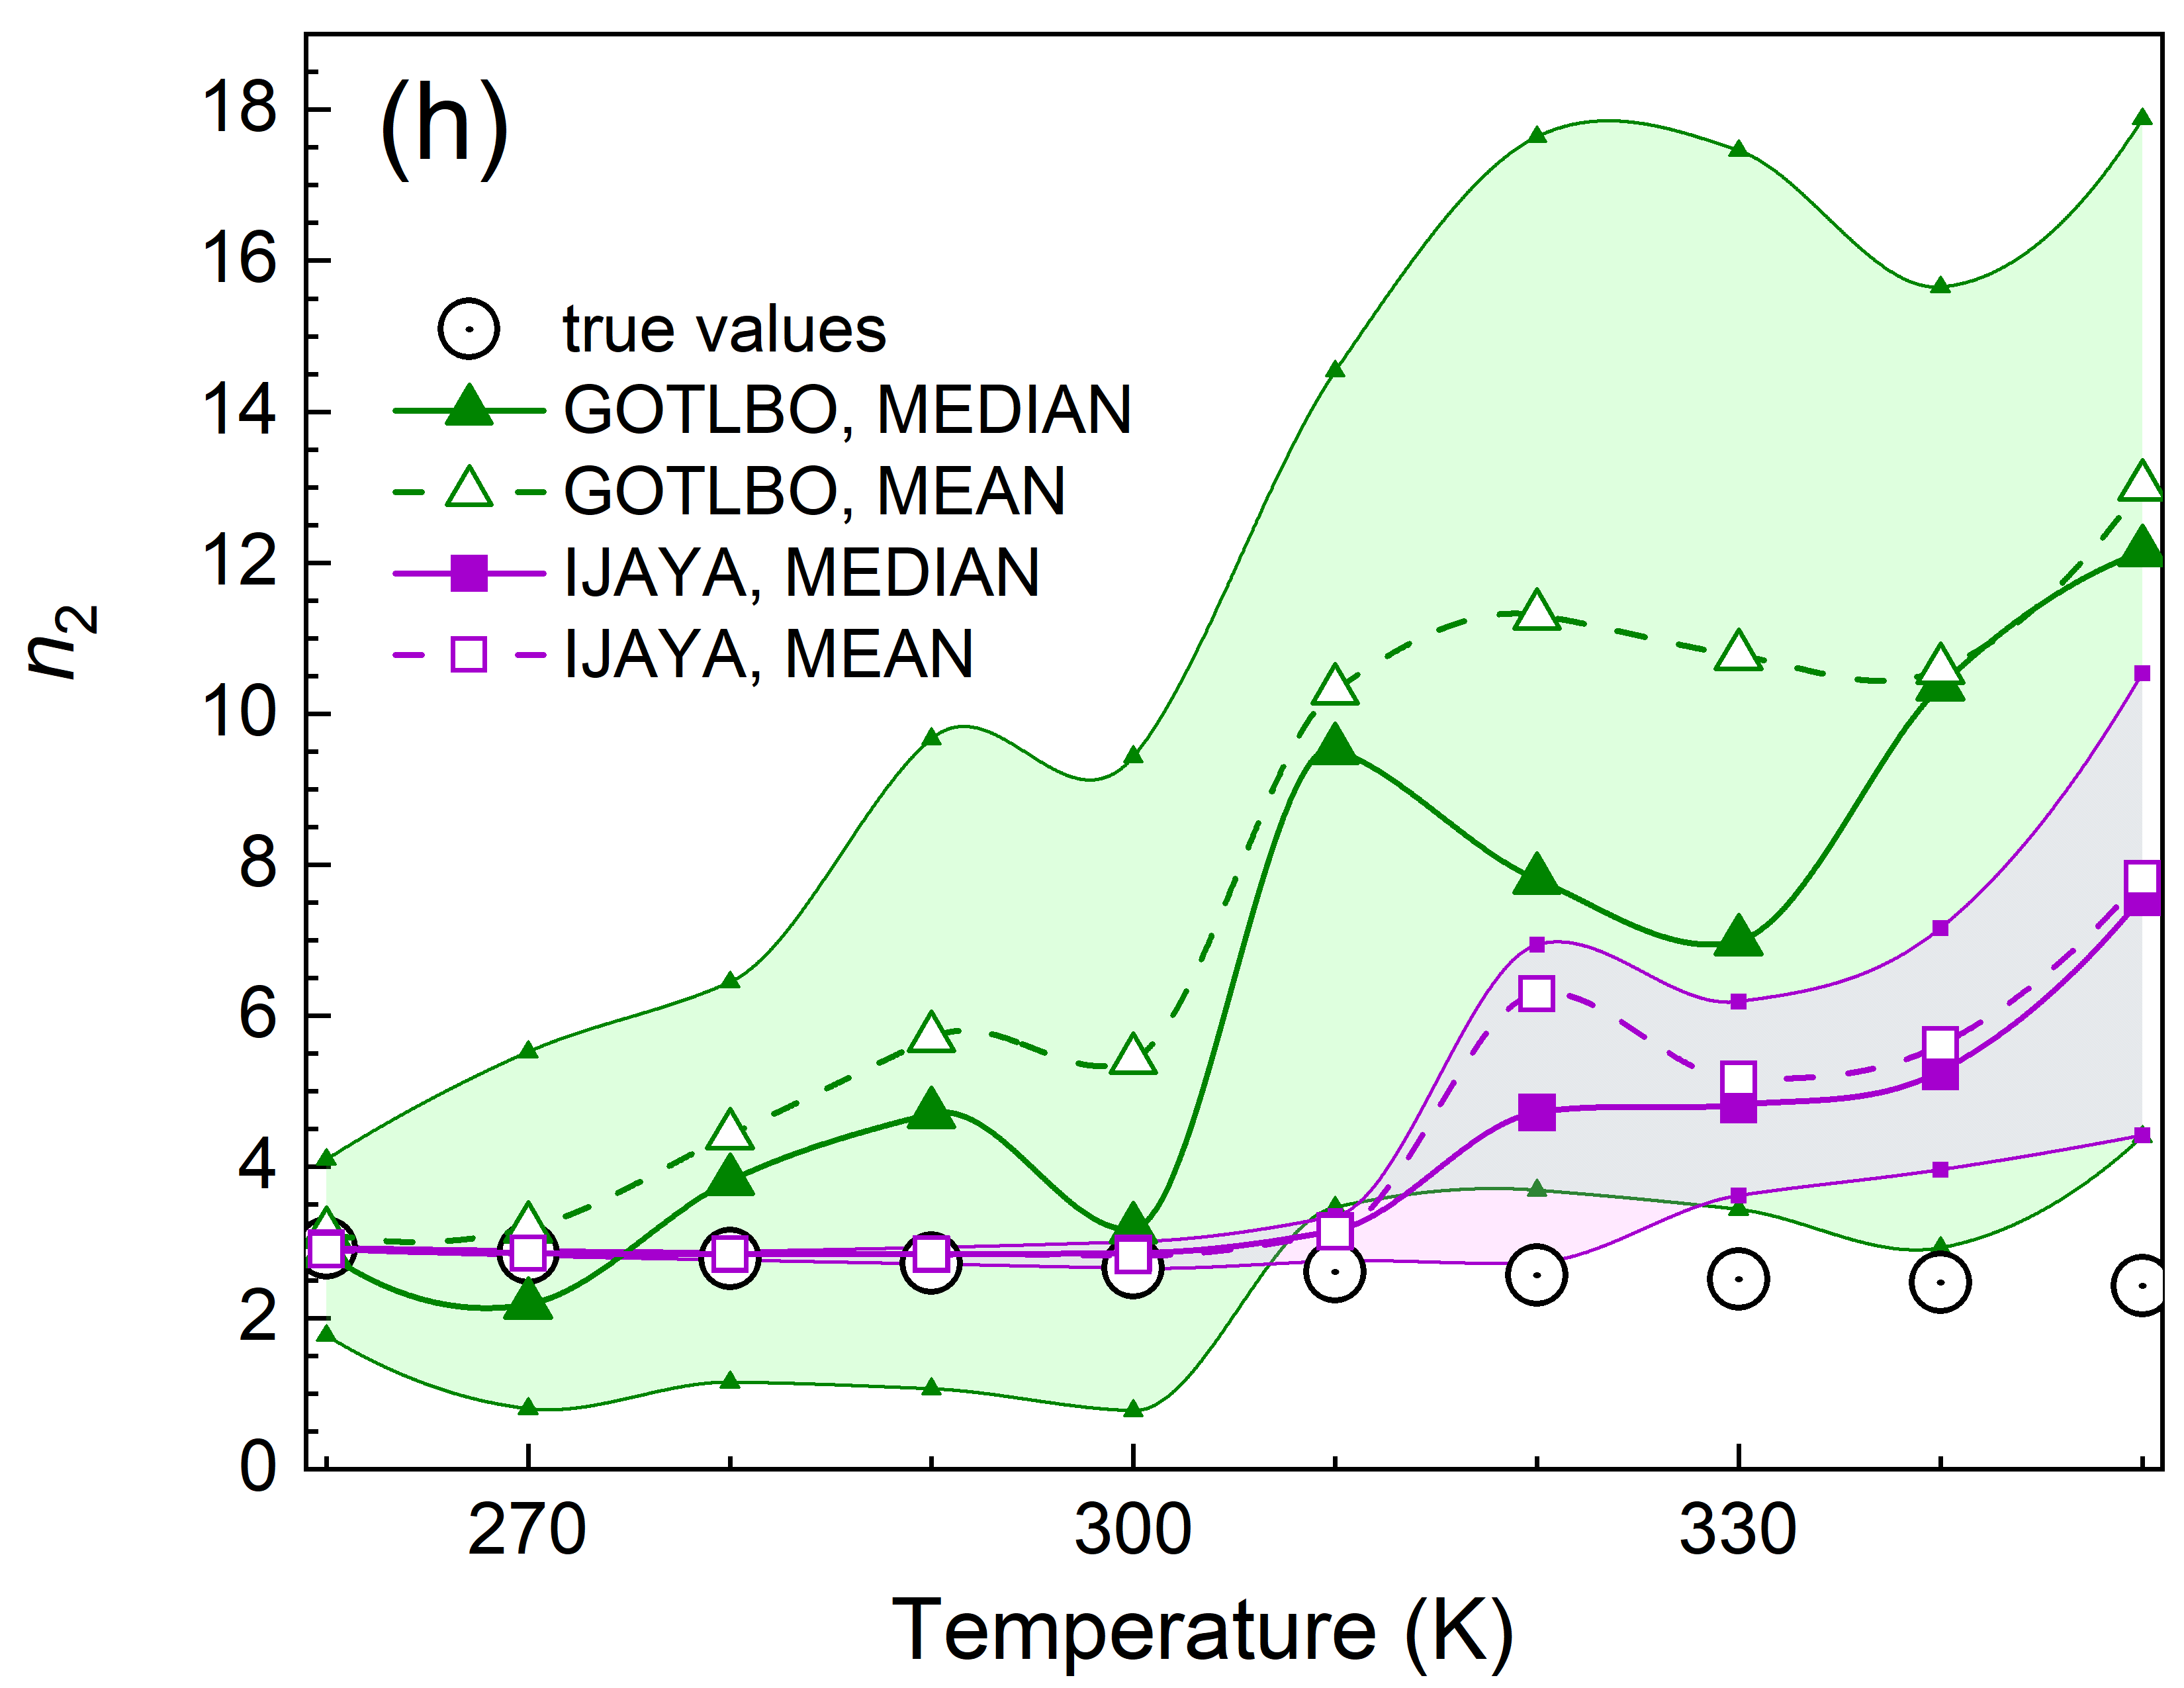
\includegraphics[width=.32\textwidth]{AfigH}
        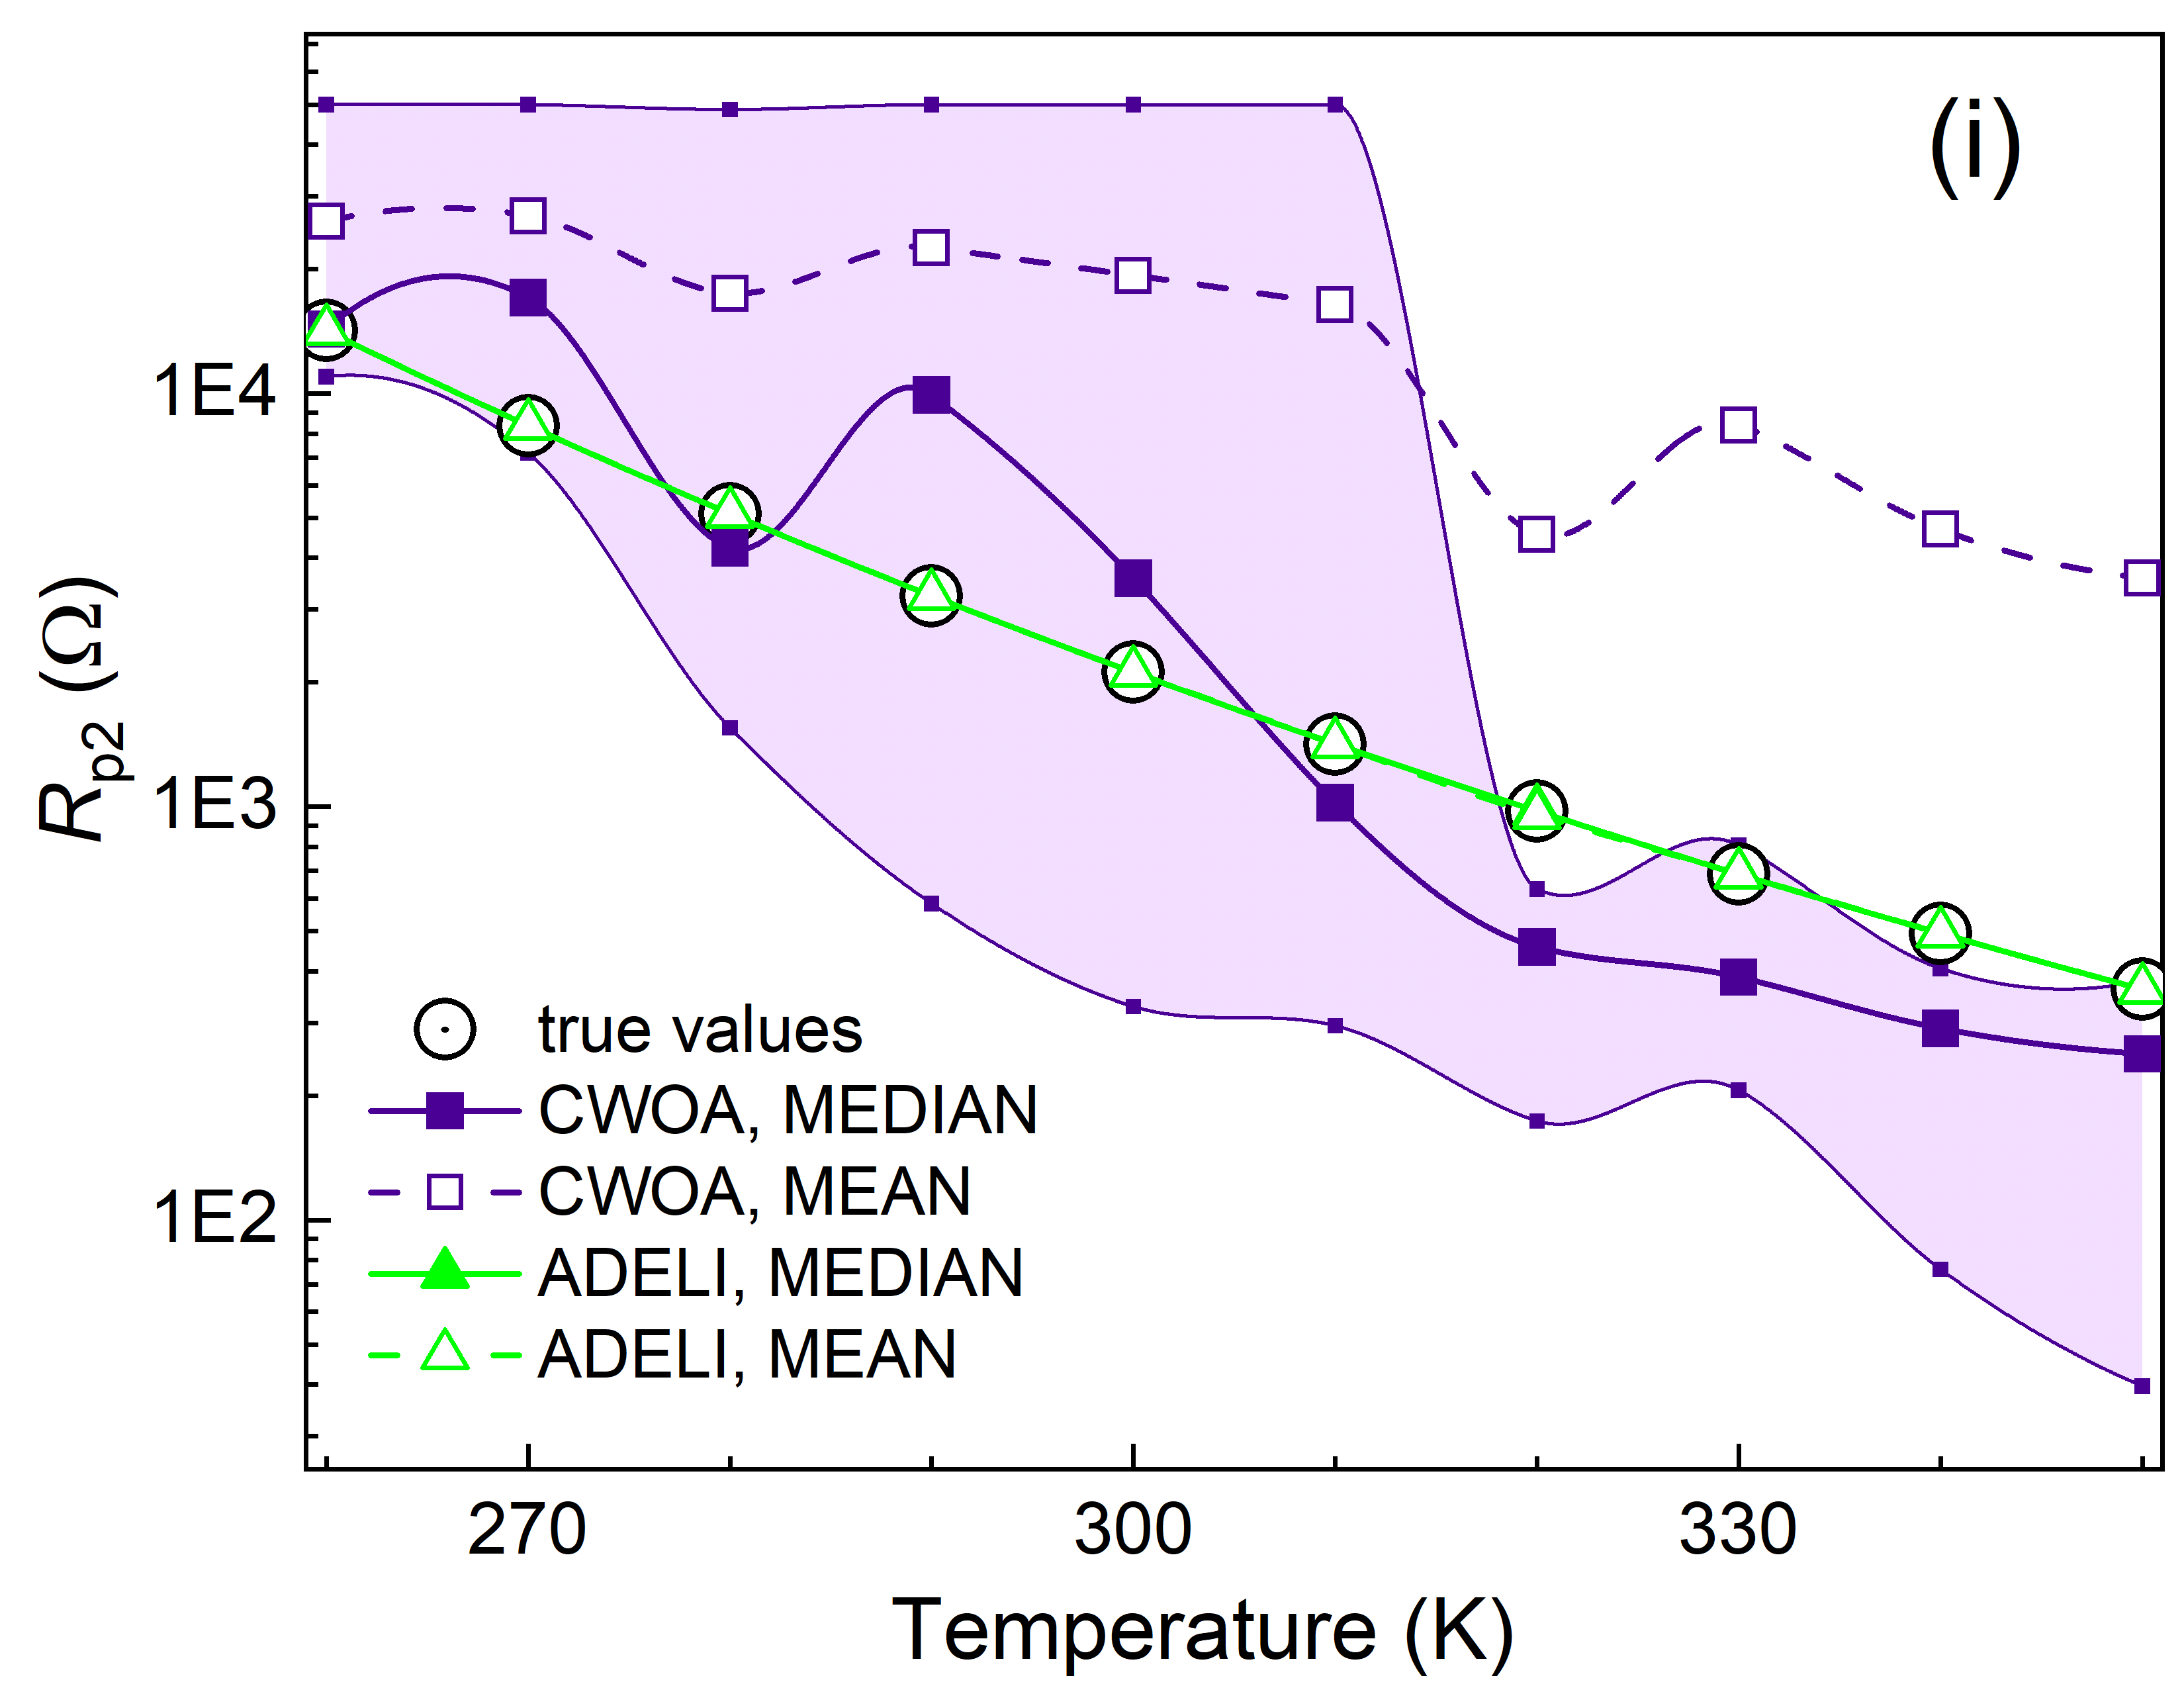
\includegraphics[width=.32\textwidth]{AfigI}
		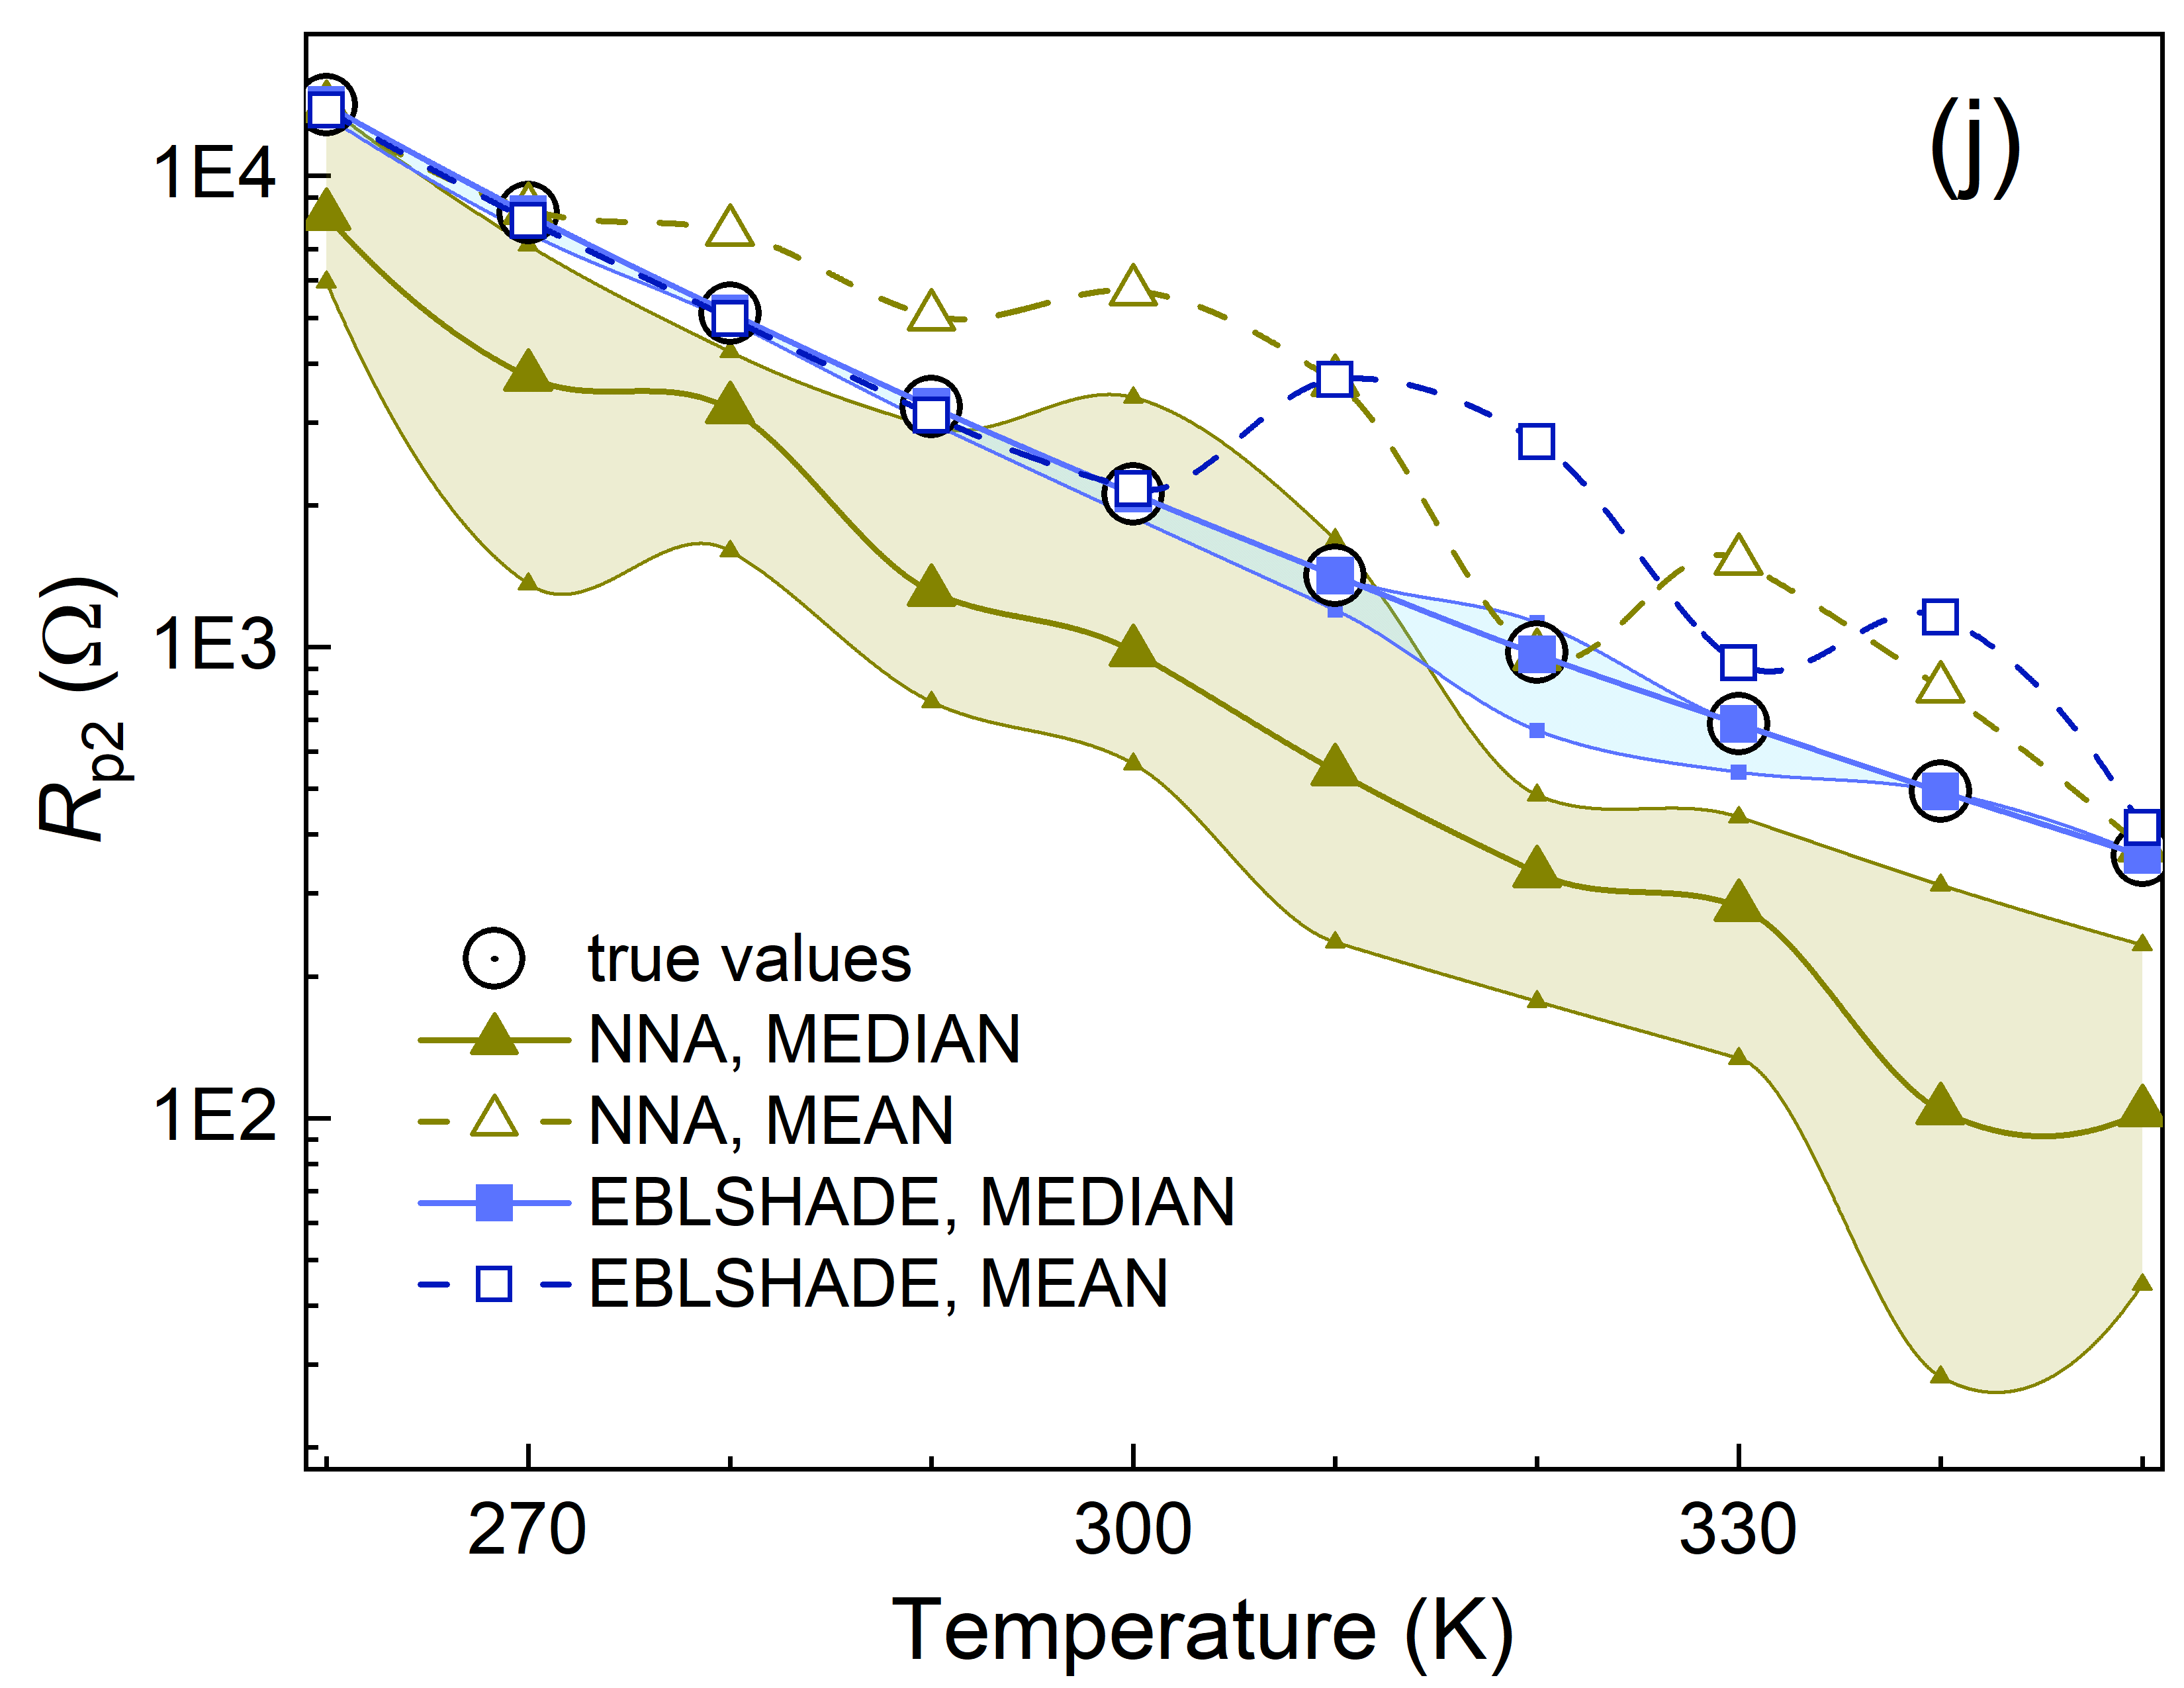
\includegraphics[width=.32\textwidth]{AfigJ}
        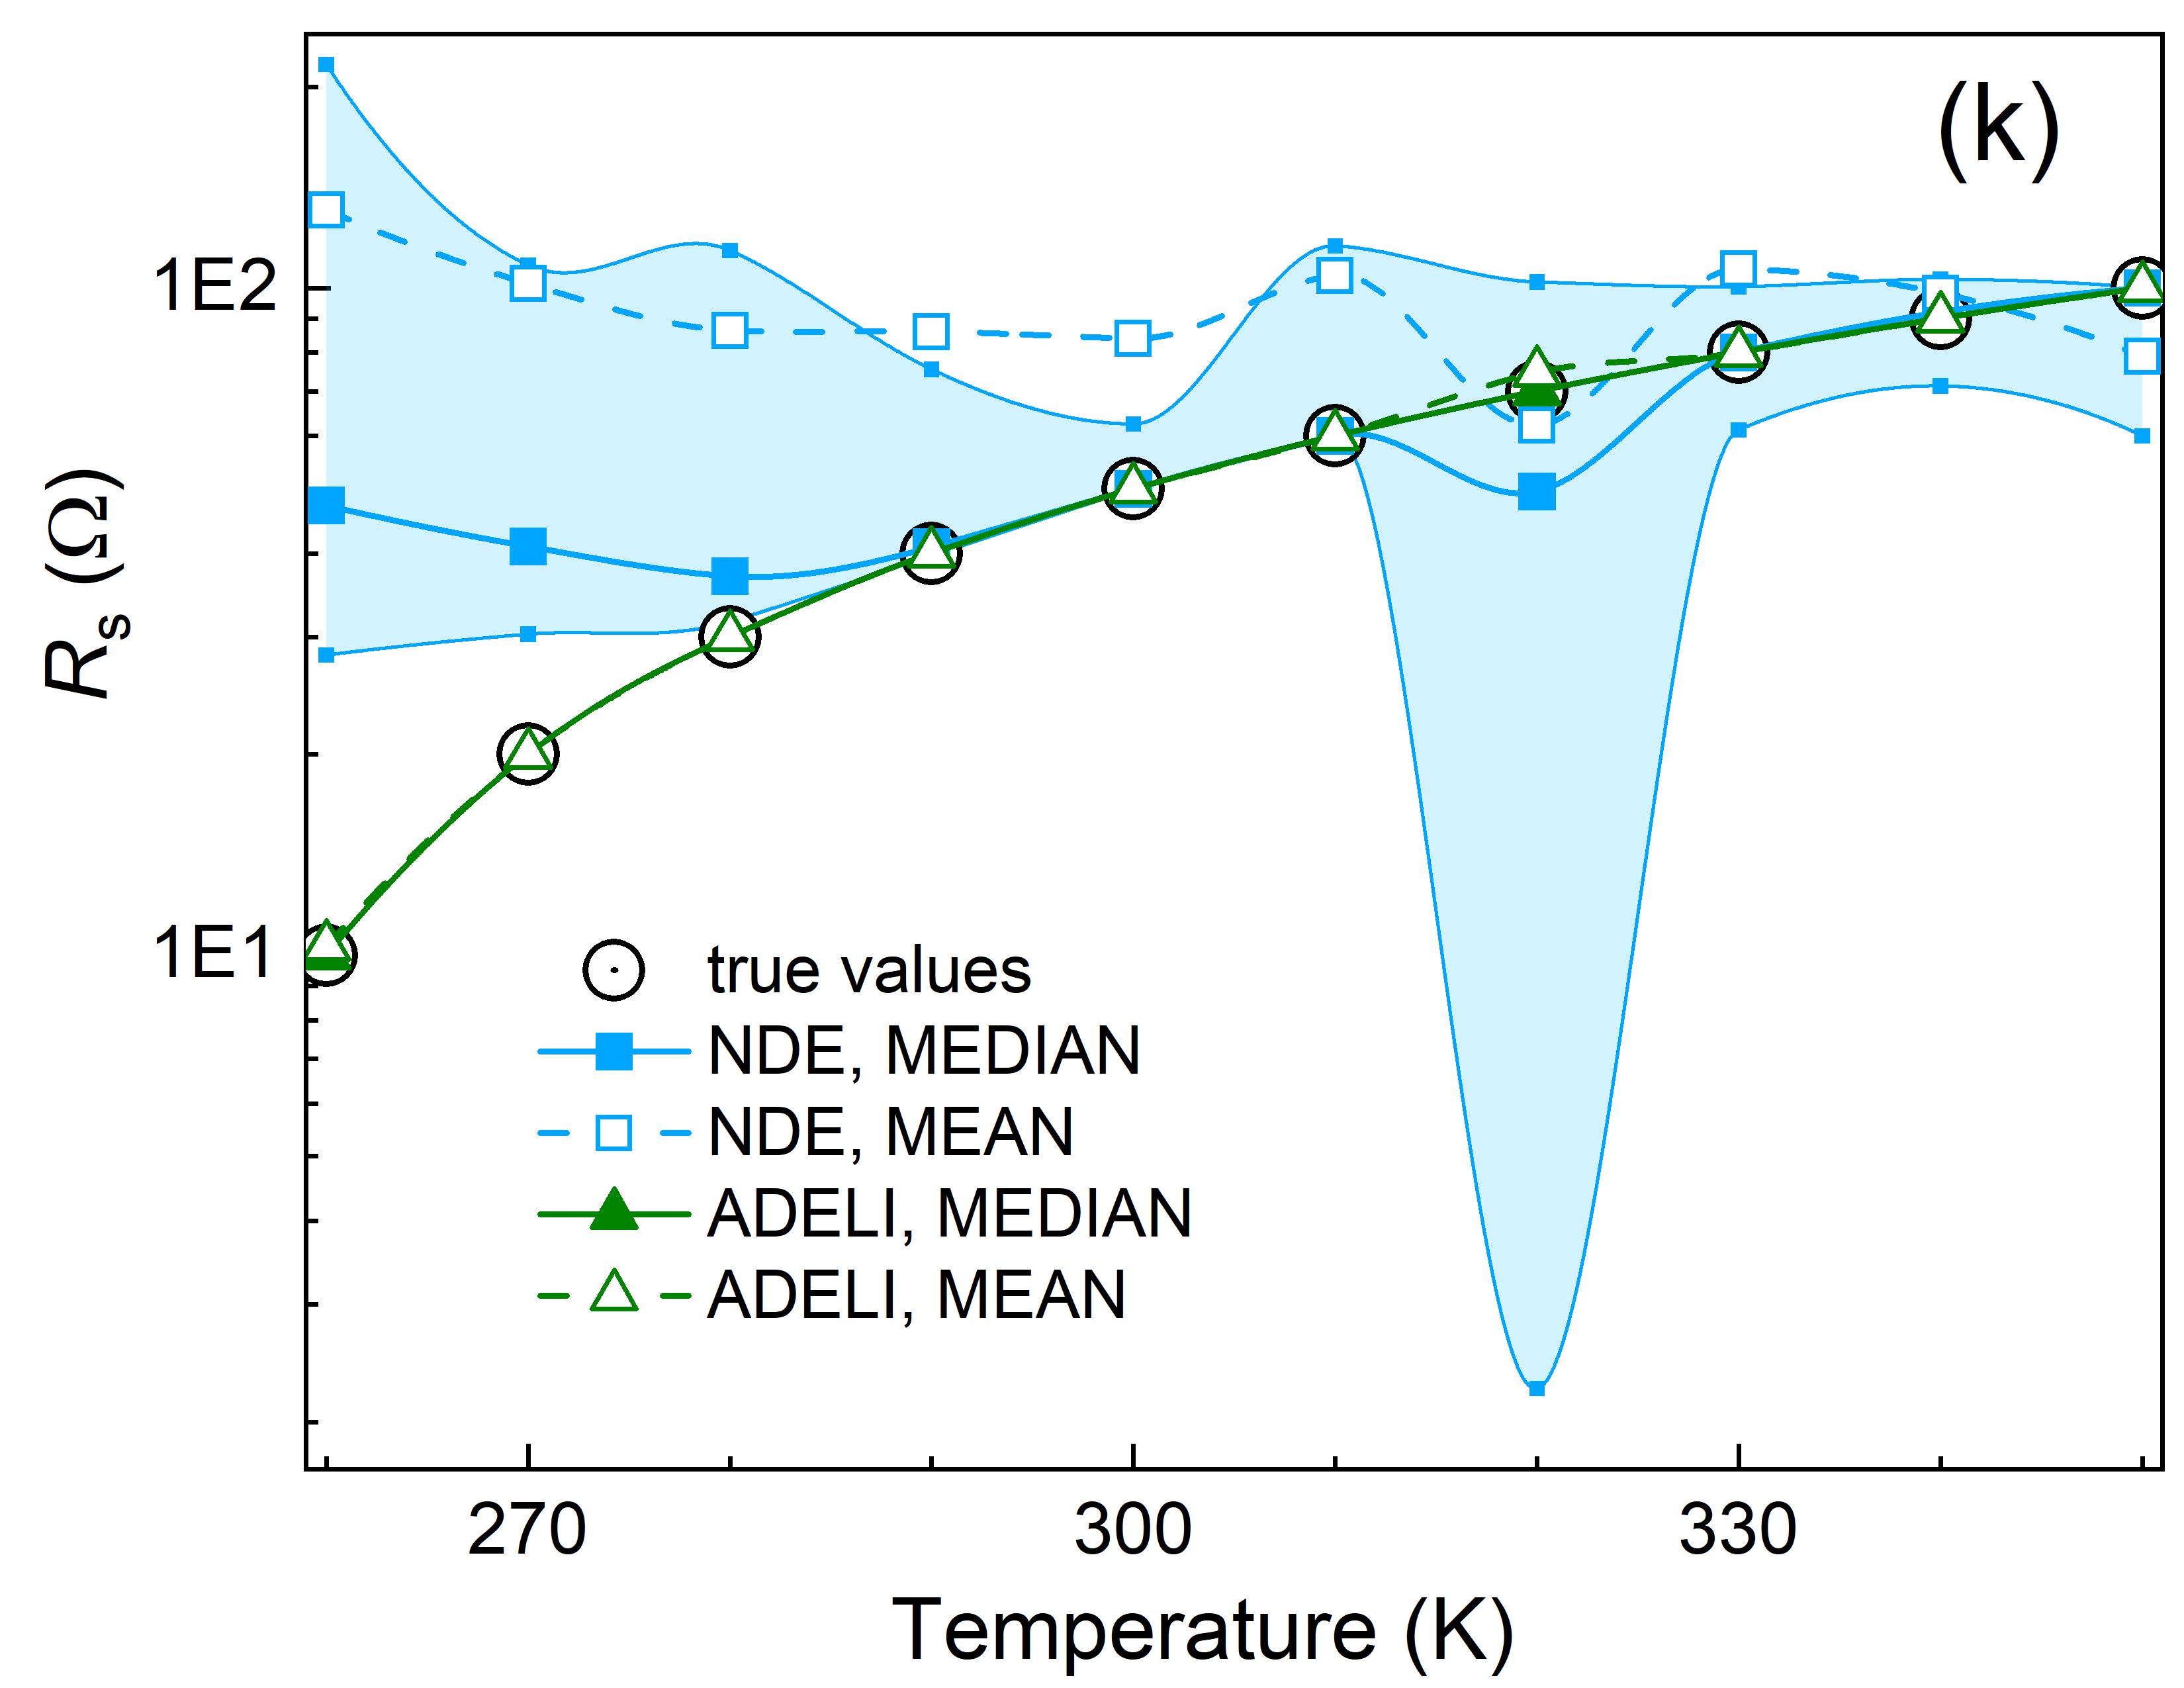
\includegraphics[width=.32\textwidth]{AfigK}
        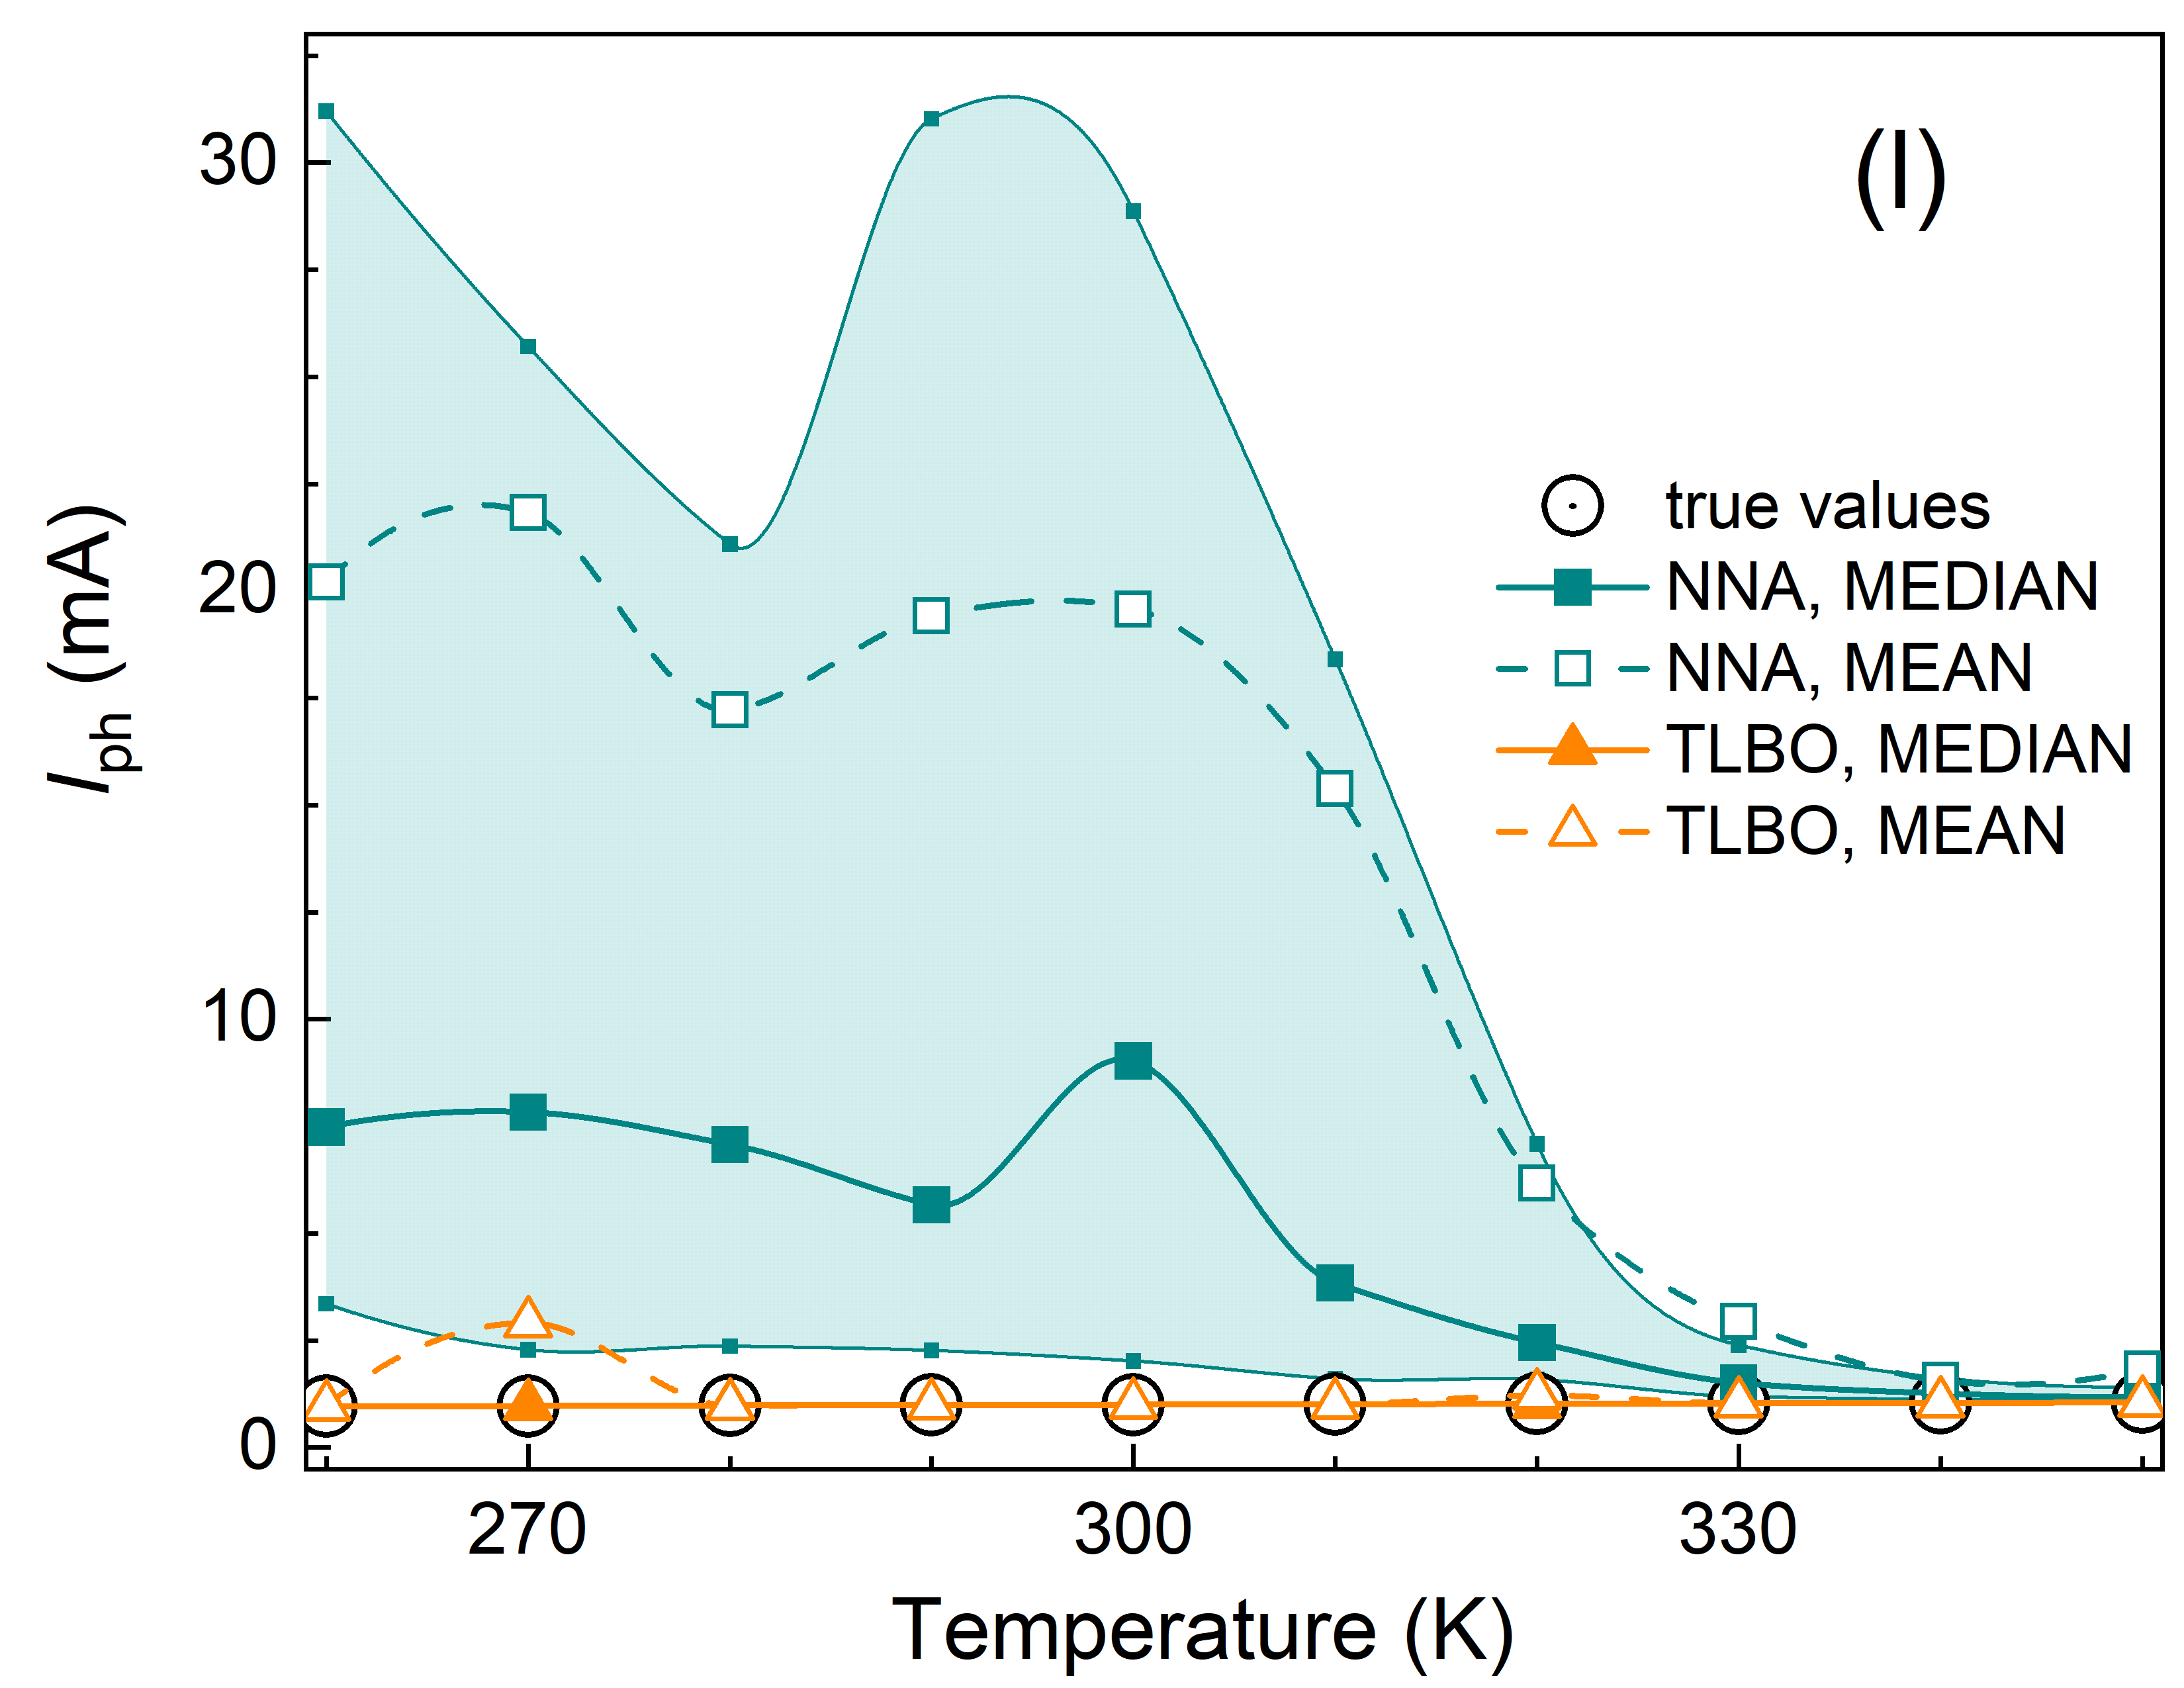
\includegraphics[width=.32\textwidth]{AfigL}
		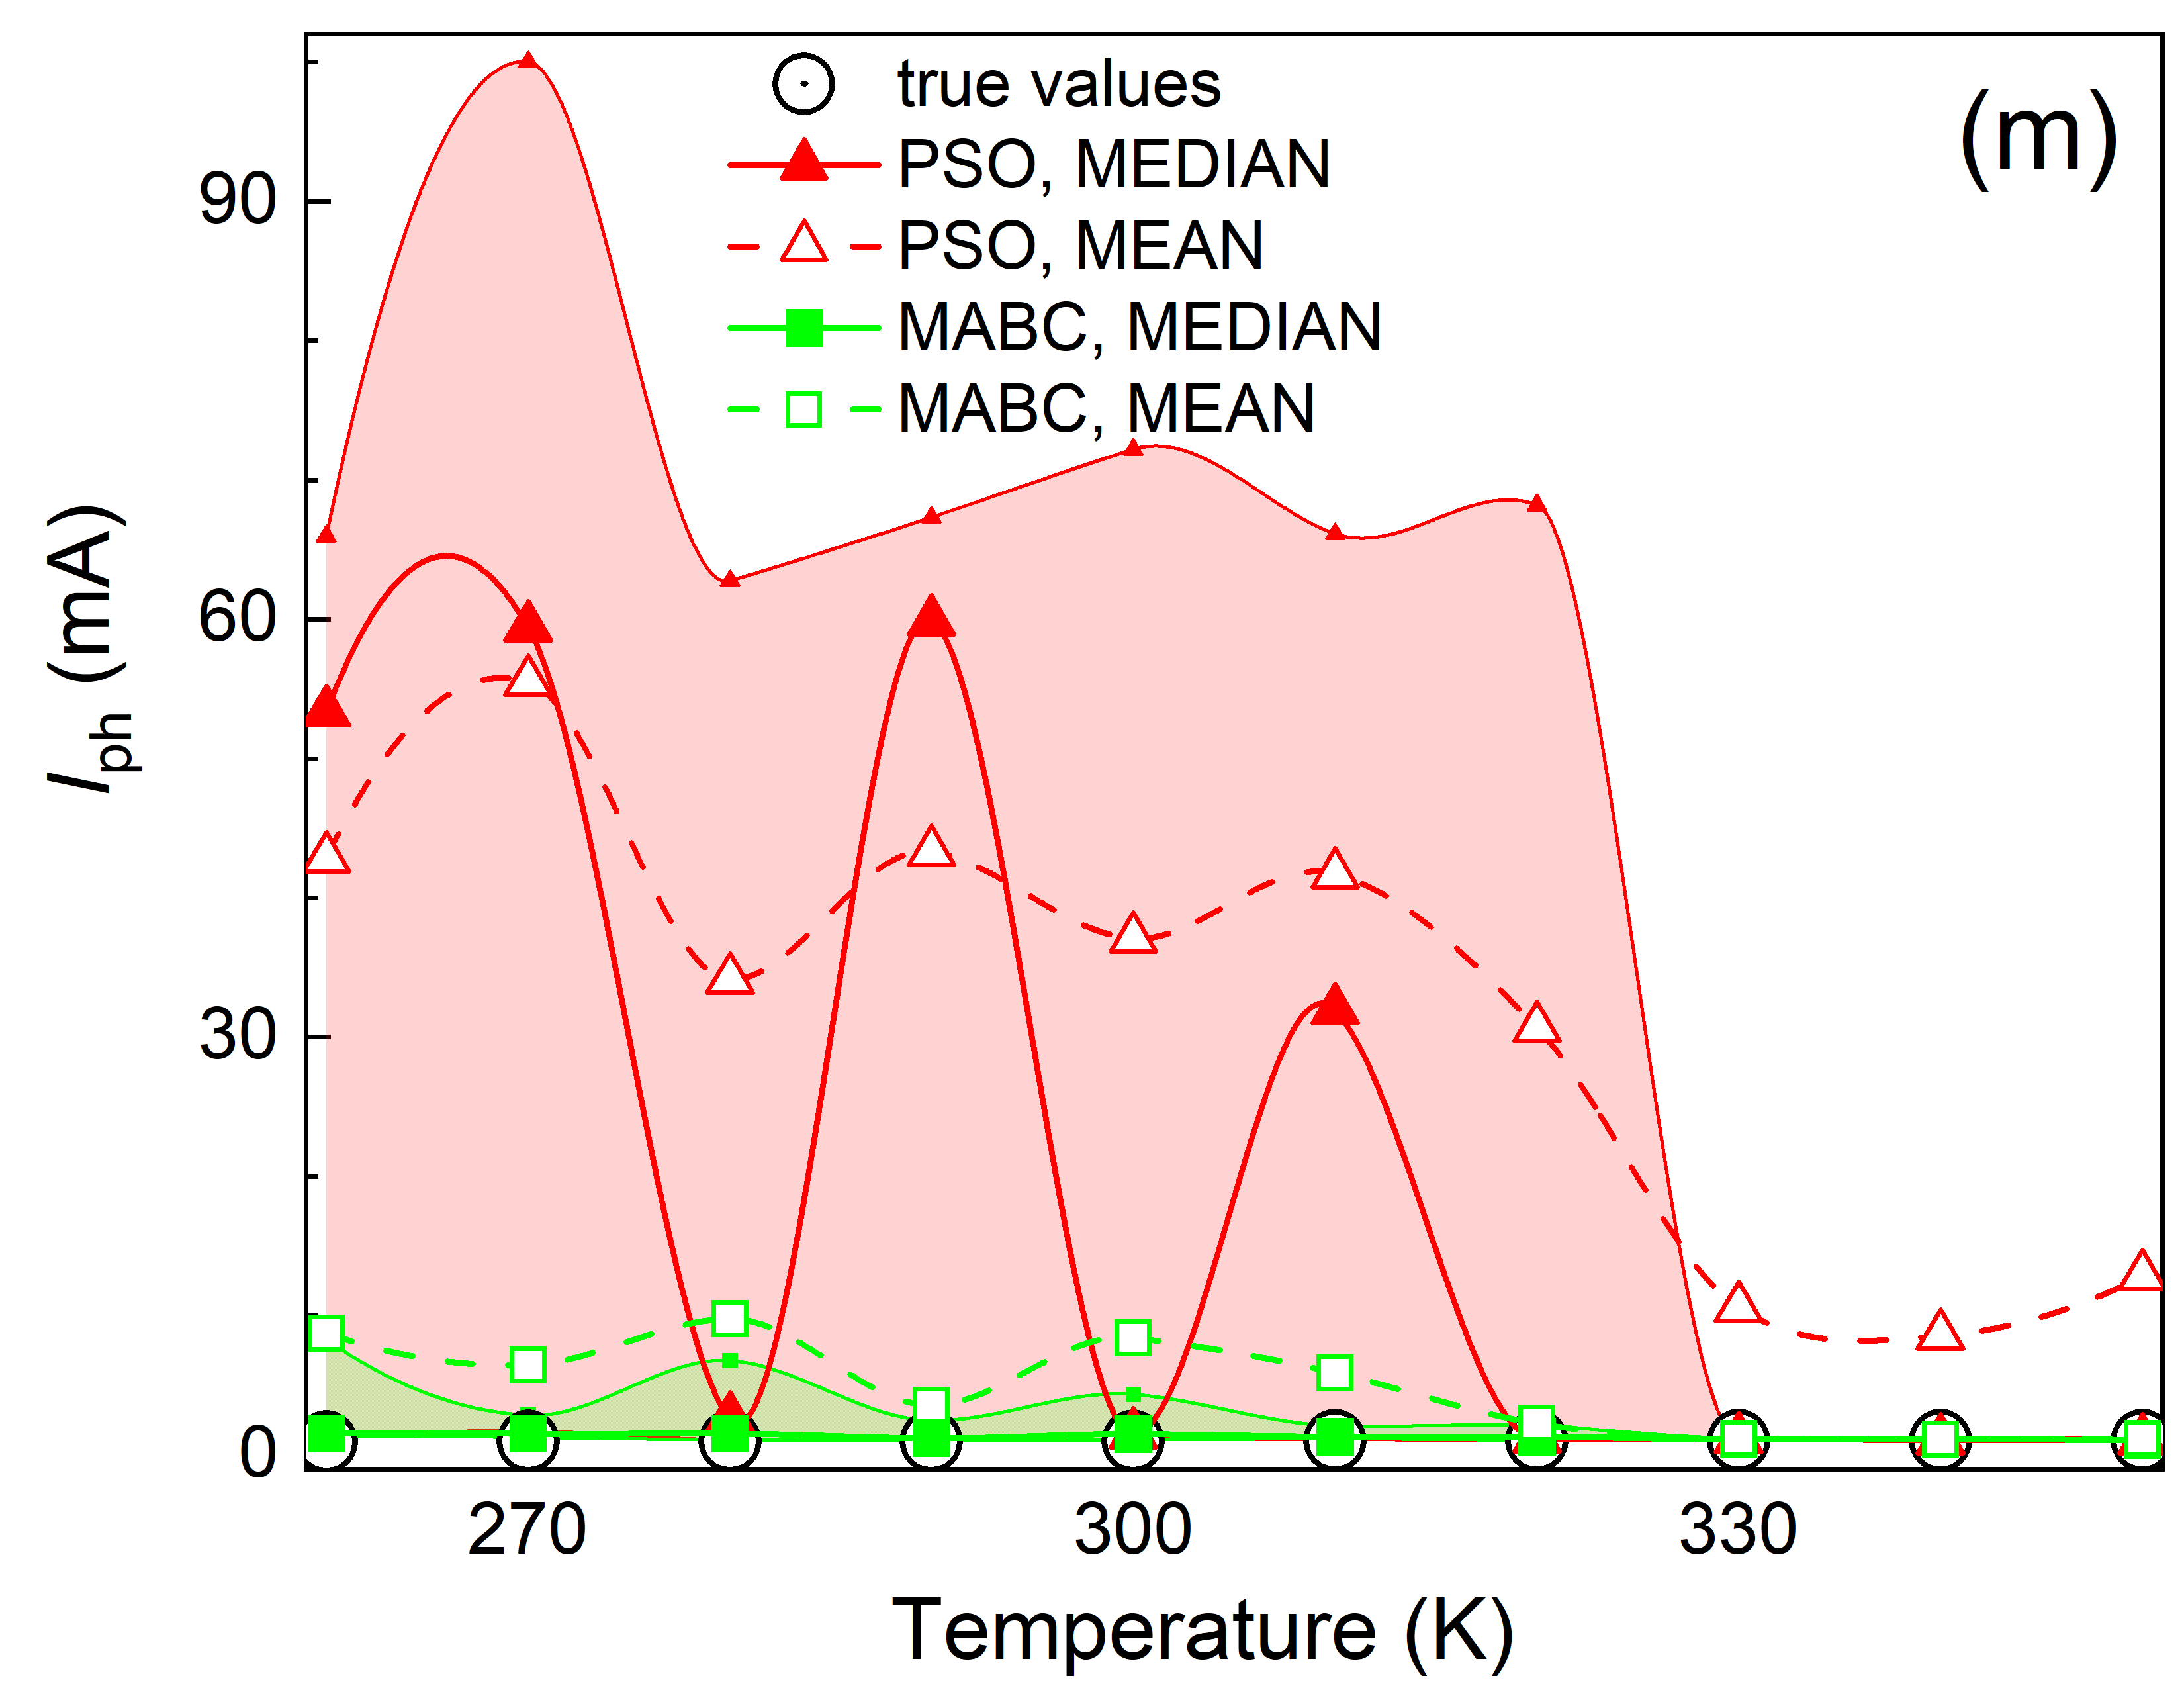
\includegraphics[width=.32\textwidth]{AfigM}
        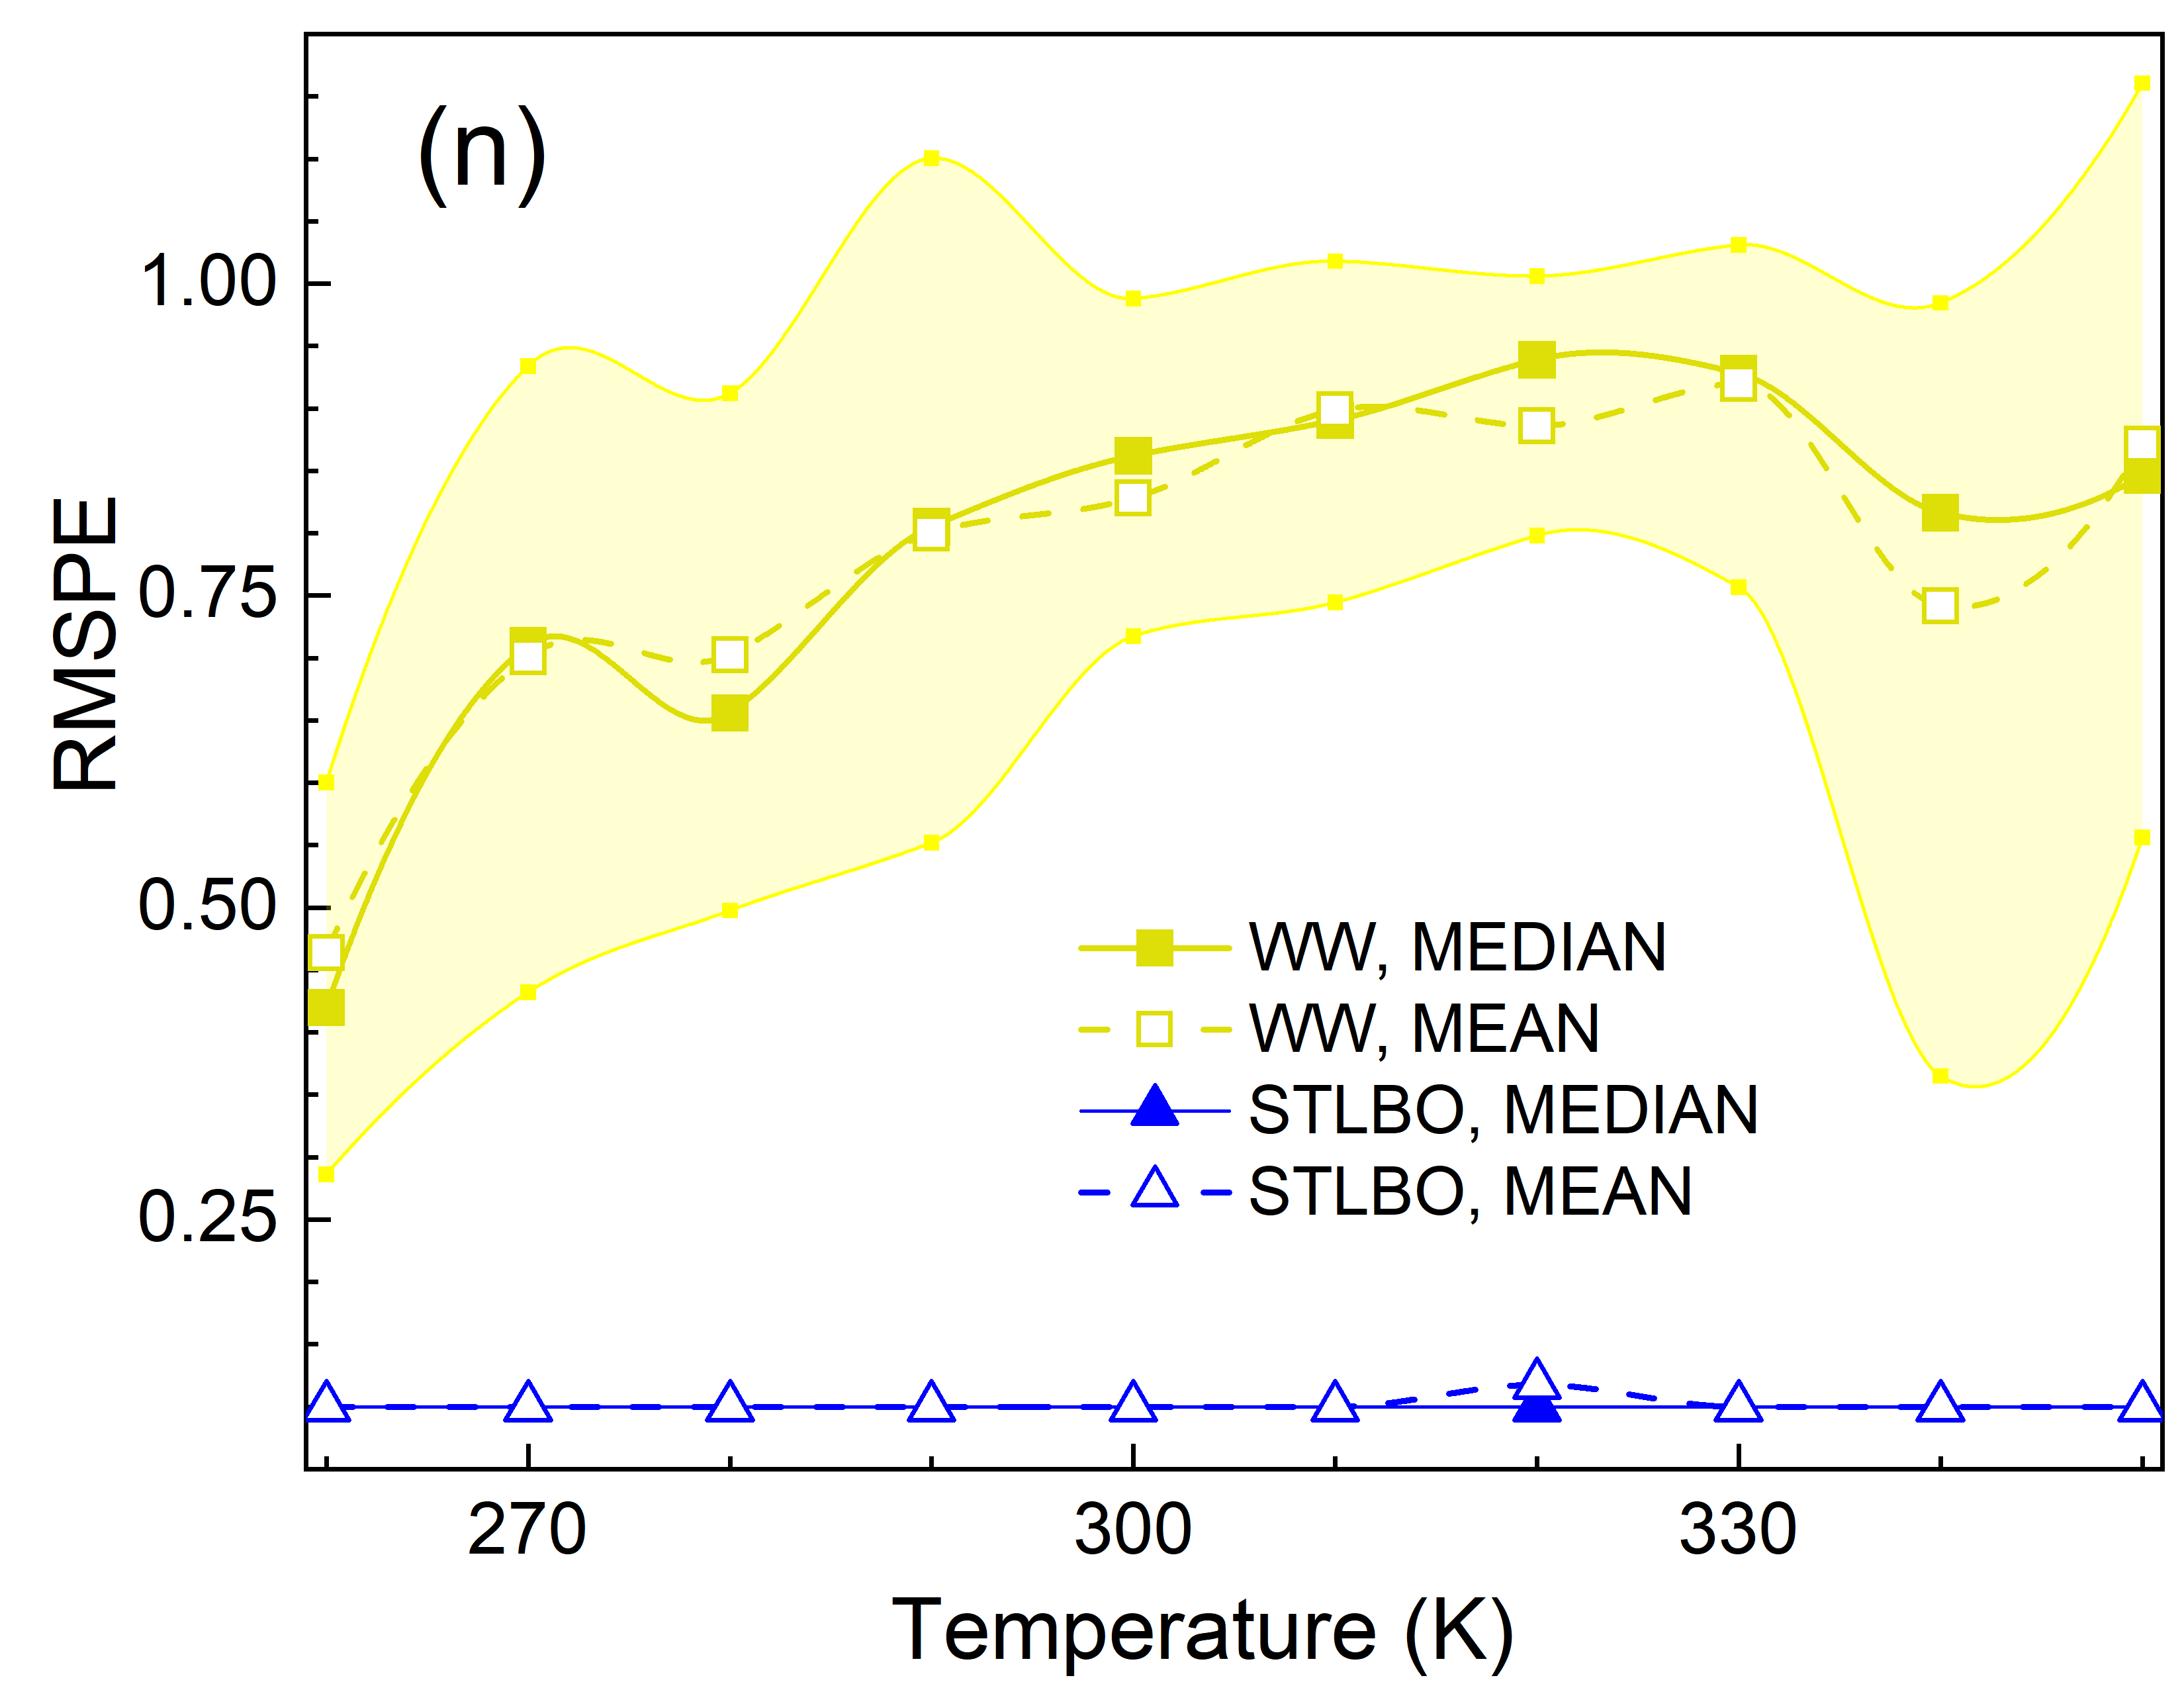
\includegraphics[width=.32\textwidth]{AfigN}
        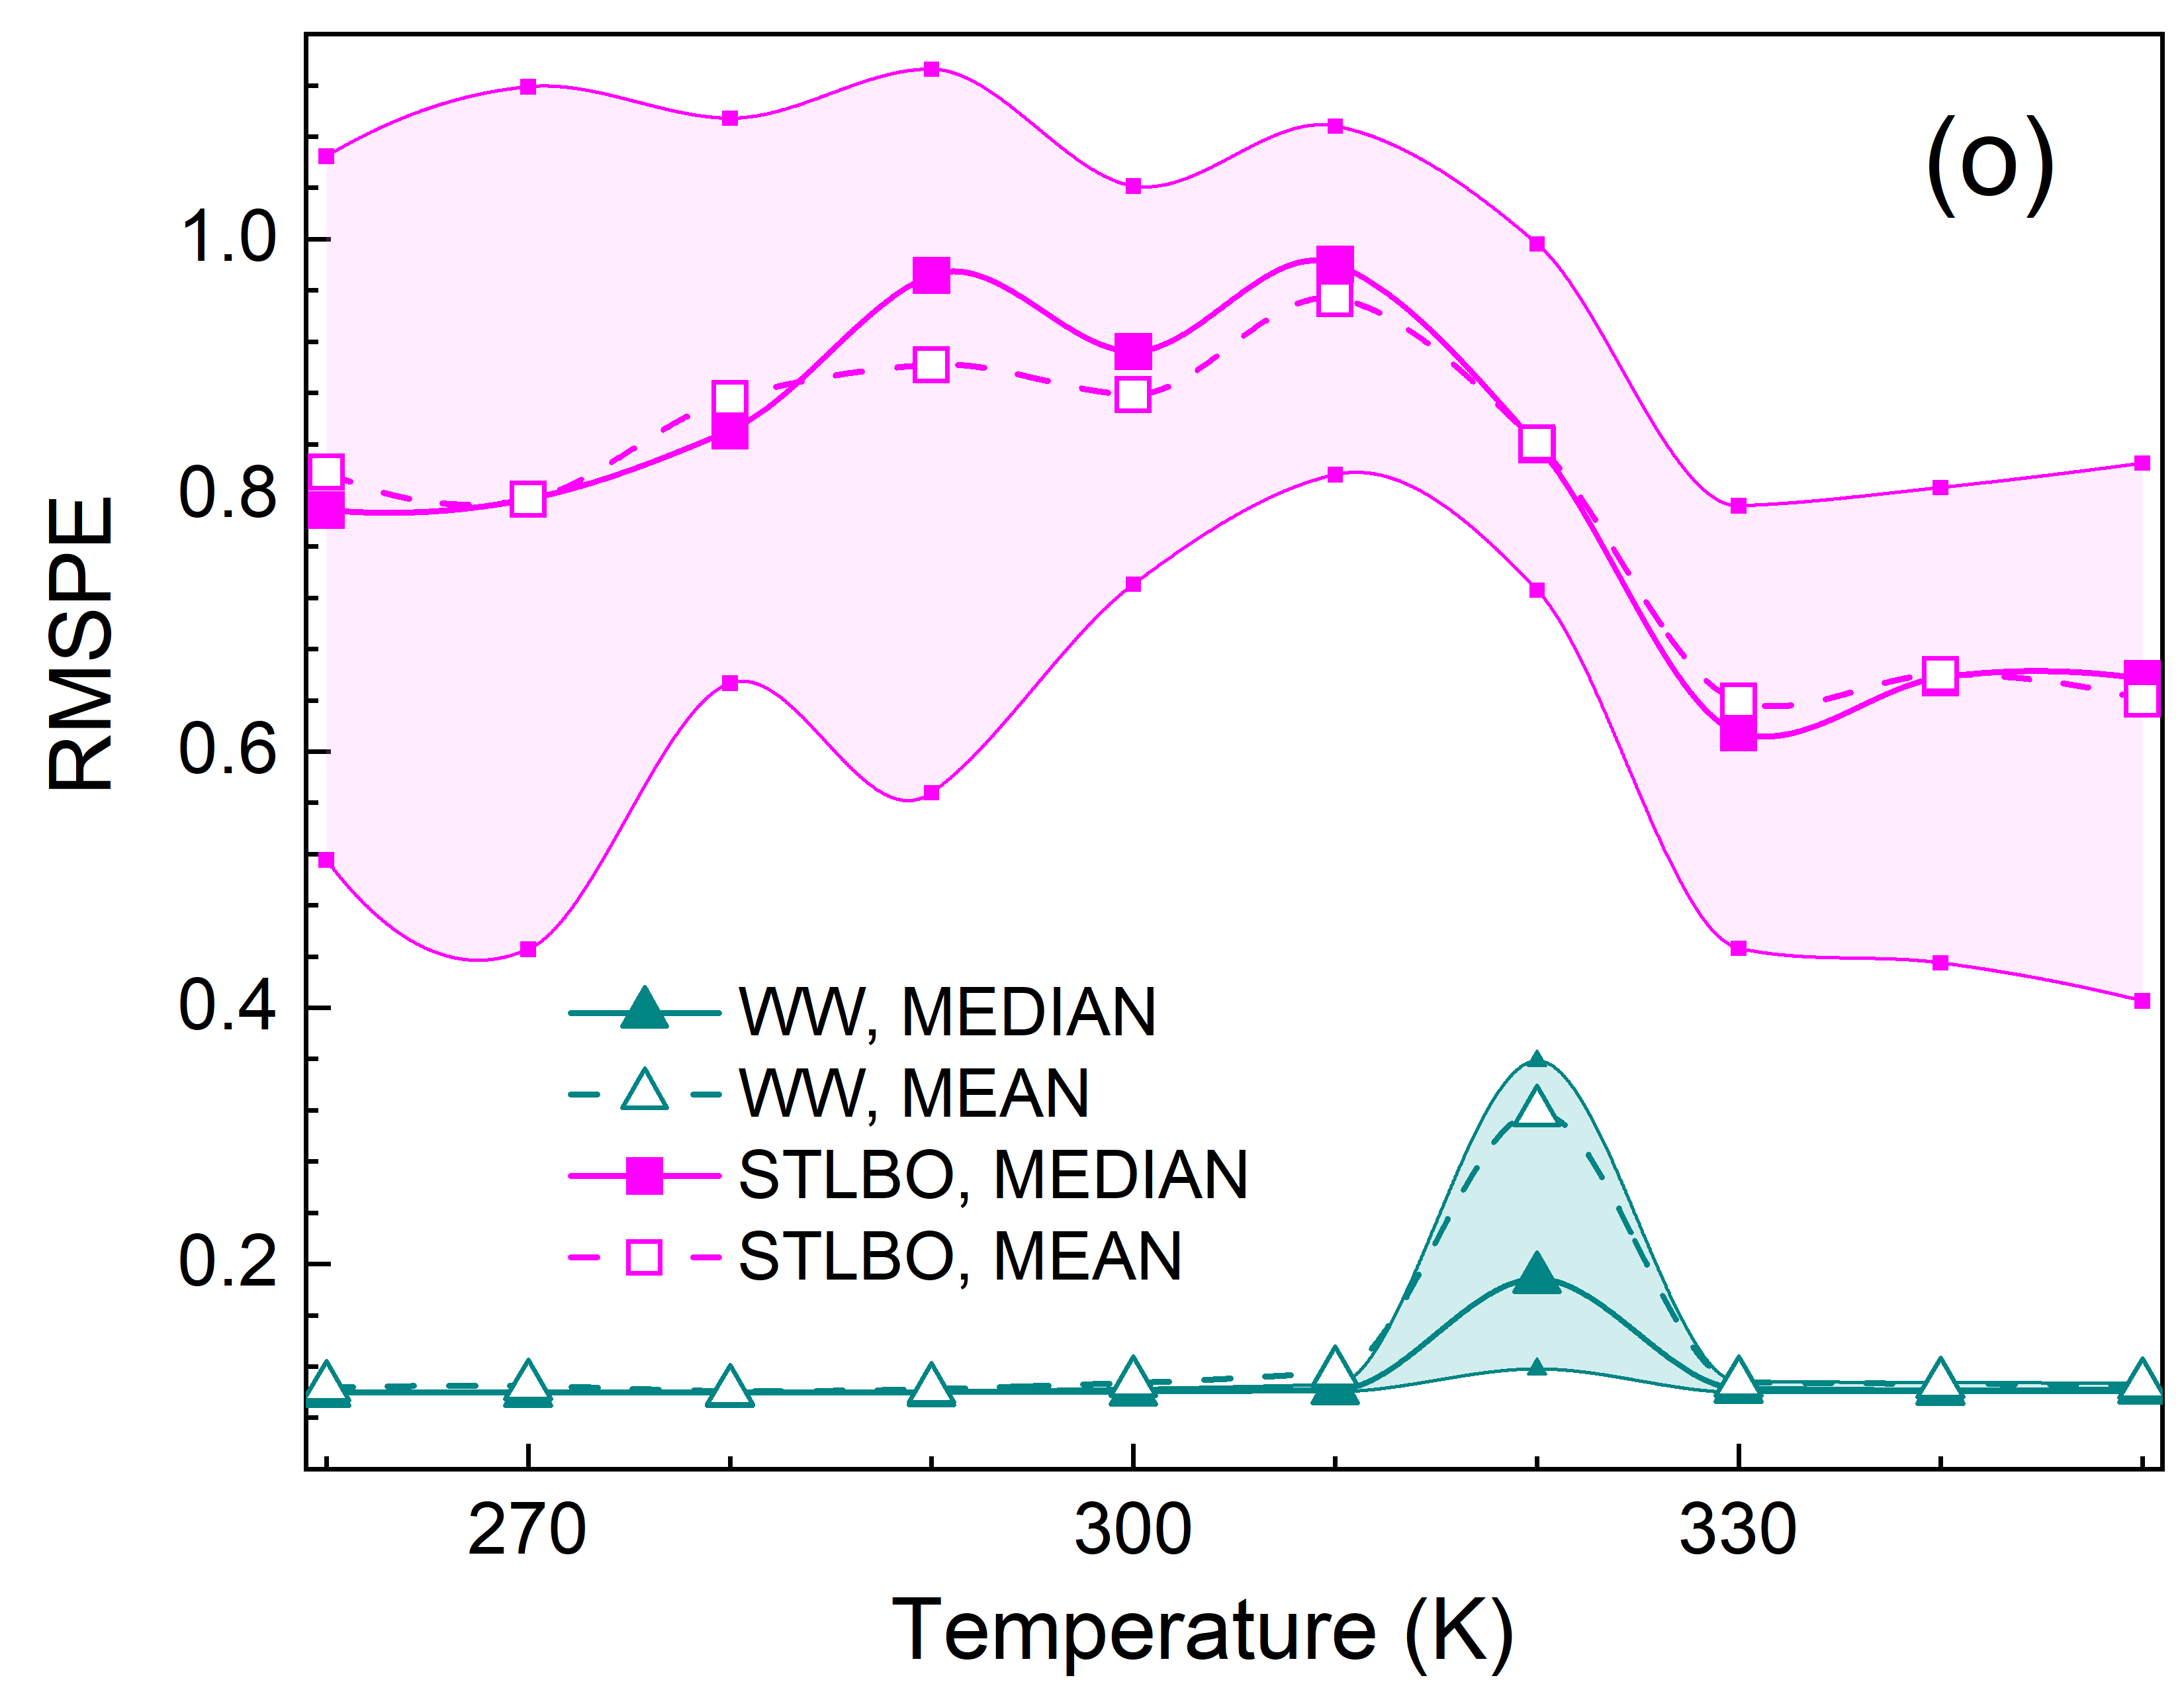
\includegraphics[width=.32\textwidth]{AfigO}
	  \caption{Dependences of the $I_{01}$ (a, b), $n_1$ (c), $R_\mathrm{p1}$ (d), $I_{02}$ (e, f),
               $n_2$ (g, h), $R_\mathrm{p2}$ (i, j), $R_\mathrm{s}$ (k), $I_\mathrm{ph}$ (l, m), and RMSPE (n, o)
               estimation by different algorithm on the synthesis temperature.
               The IV-set is used.
               The circles represent the values, which have been used in IV curve simulations,
               the filled marks represent the median values, and the empty marks represent the mean values.
               The colored regions correspond to the IQR.
               The lines only serve as guide to the eye.
               }\label{figTDepIVset}
\end{figure*}

Fig.~\ref{figSetIV} shows several typical fitting results of a set of synthetic \emph{IV} curves
simulated according to the opposed two-diode model using the parameter values described in Sec.~\ref{SetIV}.
A more comprehensive and enhanced version, including the fitting results obtained using each algorithm,
is provided in the supplementary materials (figure S4).
Similar to the single--\emph{IV} case, the algorithms EBLSHADE, ADELI, NDE, IJAYA, TLBO, and STLBO 
demonstrate the highest agreement between the fitting curves and the points of simulated current-voltage curves.
Fig.~\ref{figTDepIVset} represents a portion of the results obtained from evaluating solar cell parameters using various algorithms,
as well as the corresponding RMSPE data.
The supplementary material contains the temperature dependencies of all 
parameters determined by all algorithms applied --- see figures~S5-S13.
The results, including MEAN, MEDIAN, STD, and IQR, are also tabulated (table S154 in the supplementary material).


It should be noted that in several cases, the accuracy of parameter estimation depends on temperature, even for constant parameters.
For instance, as the temperature increases, 
the errors in determining $R_\mathrm{p1}$ decrease for NDE, MABC, GOTLBO, IJAYA, ISCA, and WW. 
However, under the same conditions, the estimation quality of $I_{01}$ worsens using DE, ISCA, and WW.
These results indicate that some parameter determination accuracy
depends on the value of this parameter and other parameter values.
However, the specific dependencies of parameter estimation accuracy 
for each algorithm were beyond the scope of the study. 
We aimed to determine the best algorithms only.


\begin{table*}[<options>]
\caption{The results of Wilcoxon signed-rank test with a level of significance $\alpha = 0.05$ in the IV-set case.
         The ``+'' indicated that the null hypothesis was rejected, and the control algorithm (in the row) performed better
         then the comparison algorithm (in the column).
         The ``0'' indicates to rejection of the hypothesis about outperforming the control algorithm.
         }\label{tblWilIVset}
\begin{tabular*}{\tblwidth}{@{}LCCCCCCCCCCCCCCC@{}}
\toprule
Control & \multicolumn{14}{C}{Comparison algorithm}&Total \\
algorithm  &DE&EBLSHADE&ADELI&NDE&MABC&TLBO&GOTLBO&STLBO&PSO&IJAYA&ISCA&NNA&CWOA&WW&$(+/=/-)$\\ % Table header row
\midrule
DE&$\blacksquare$&0&0&0&+&0&+&0&+&0&+&+&+&+&7/0/6\\
EBLSHADE&+&$\blacksquare$&0&+&+&0&+&0&+&+&+&+&+&+&10/0/3\\
ADELI&+&+&$\blacksquare$&+&+&+&+&+&+&+&+&+&+&+&13/0/0\\
NDE&+&0&0&$\blacksquare$&+&0&+&0&+&+&+&+&+&+&9/0/4\\
MABC&0&0&0&0&$\blacksquare$&0&+&0&+&0&+&+&+&+&6/0/7\\
TLBO&+&+&0&+&+&$\blacksquare$&+&0&+&+&+&+&+&+&11/1/1\\
GOTLBO&0&0&0&0&0&0&$\blacksquare$&0&+&0&+&+&+&+&5/0/8\\
STLBO&+&+&0&+&+&0&+&$\blacksquare$&+&+&+&+&+&+&11/1/1\\
PSO&0&0&0&0&0&0&0&0&$\blacksquare$&0&0&0&0&0&0/4/9\\
IJAYA&+&0&0&0&+&0&+&0&+&$\blacksquare$&+&+&+&+&8/0/5\\
ISCA&0&0&0&0&0&0&0&0&0&0&$\blacksquare$&0&0&0&0/3/10\\
NNA&0&0&0&0&0&0&0&0&0&0&0&$\blacksquare$&0&0&0/3/10\\
CWOA&0&0&0&0&0&0&0&0&0&0&0&0&$\blacksquare$&0&0/4/9\\
WW&0&0&0&0&0&0&0&0&0&0&0&+&0&$\blacksquare$&1/3/9\\
\bottomrule
\end{tabular*}
\end{table*}

\begin{figure}[]
	\centering
%		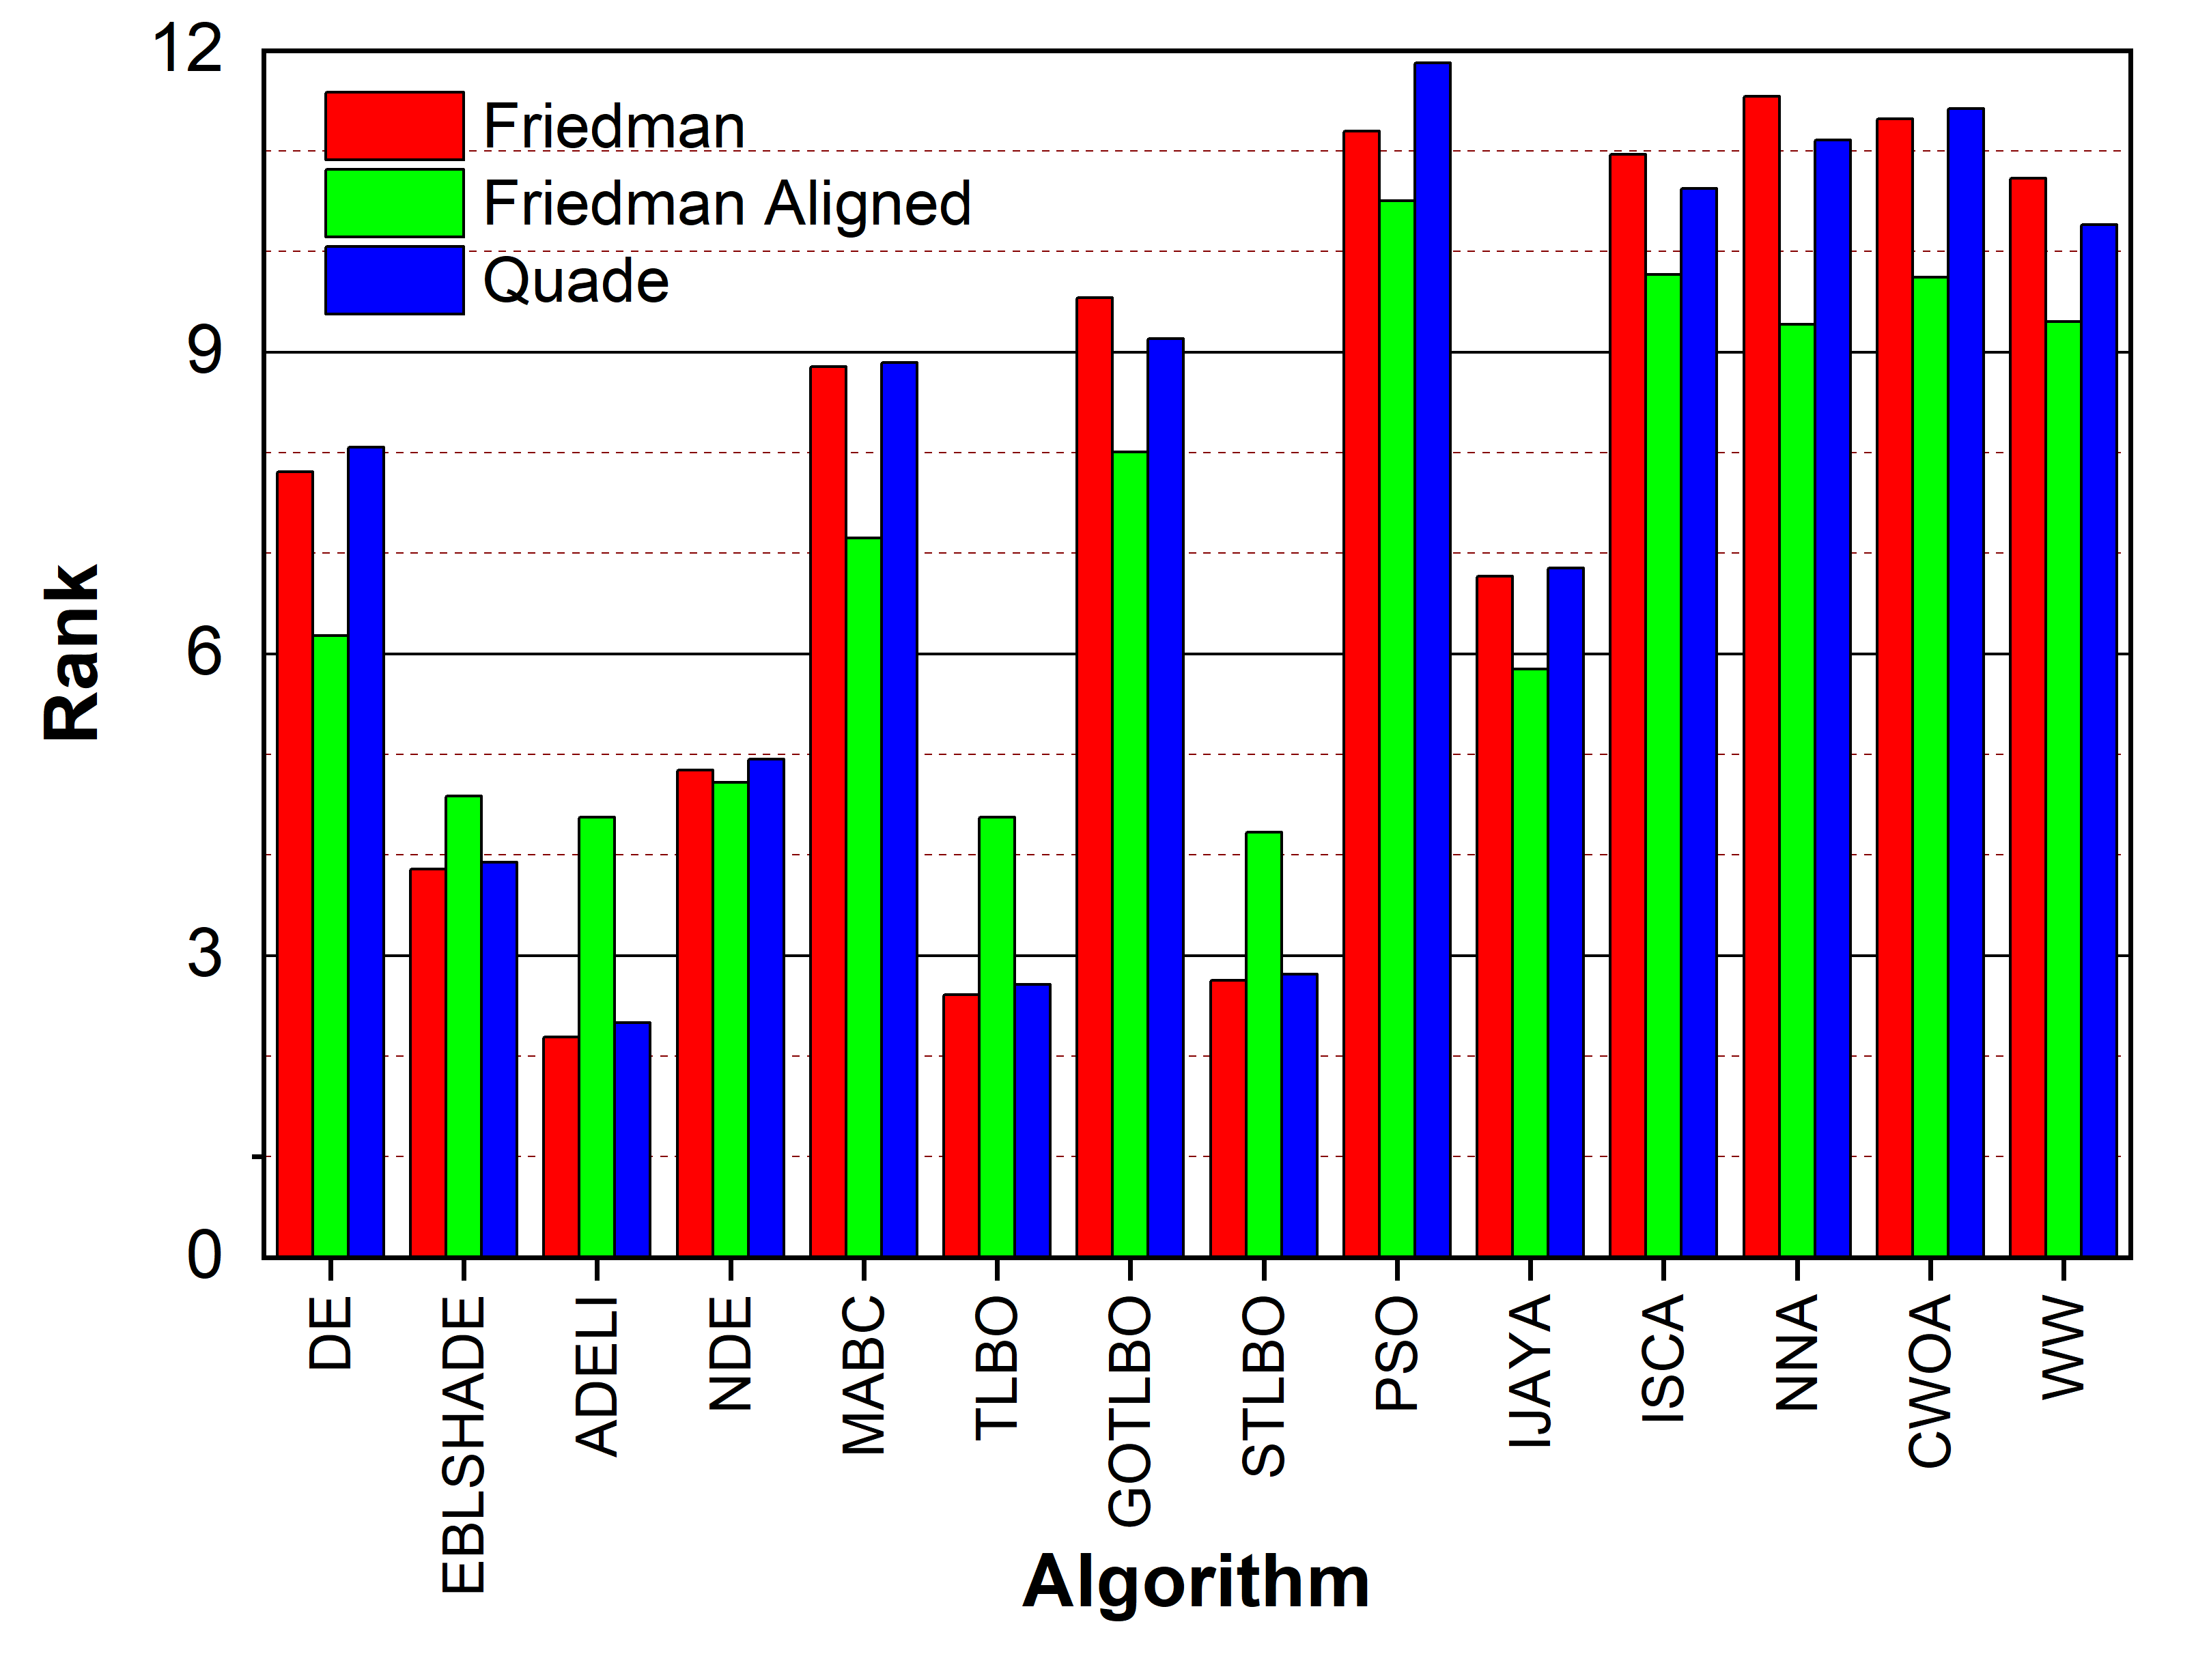
\includegraphics[width=1.0\columnwidth]{FigRankT}
		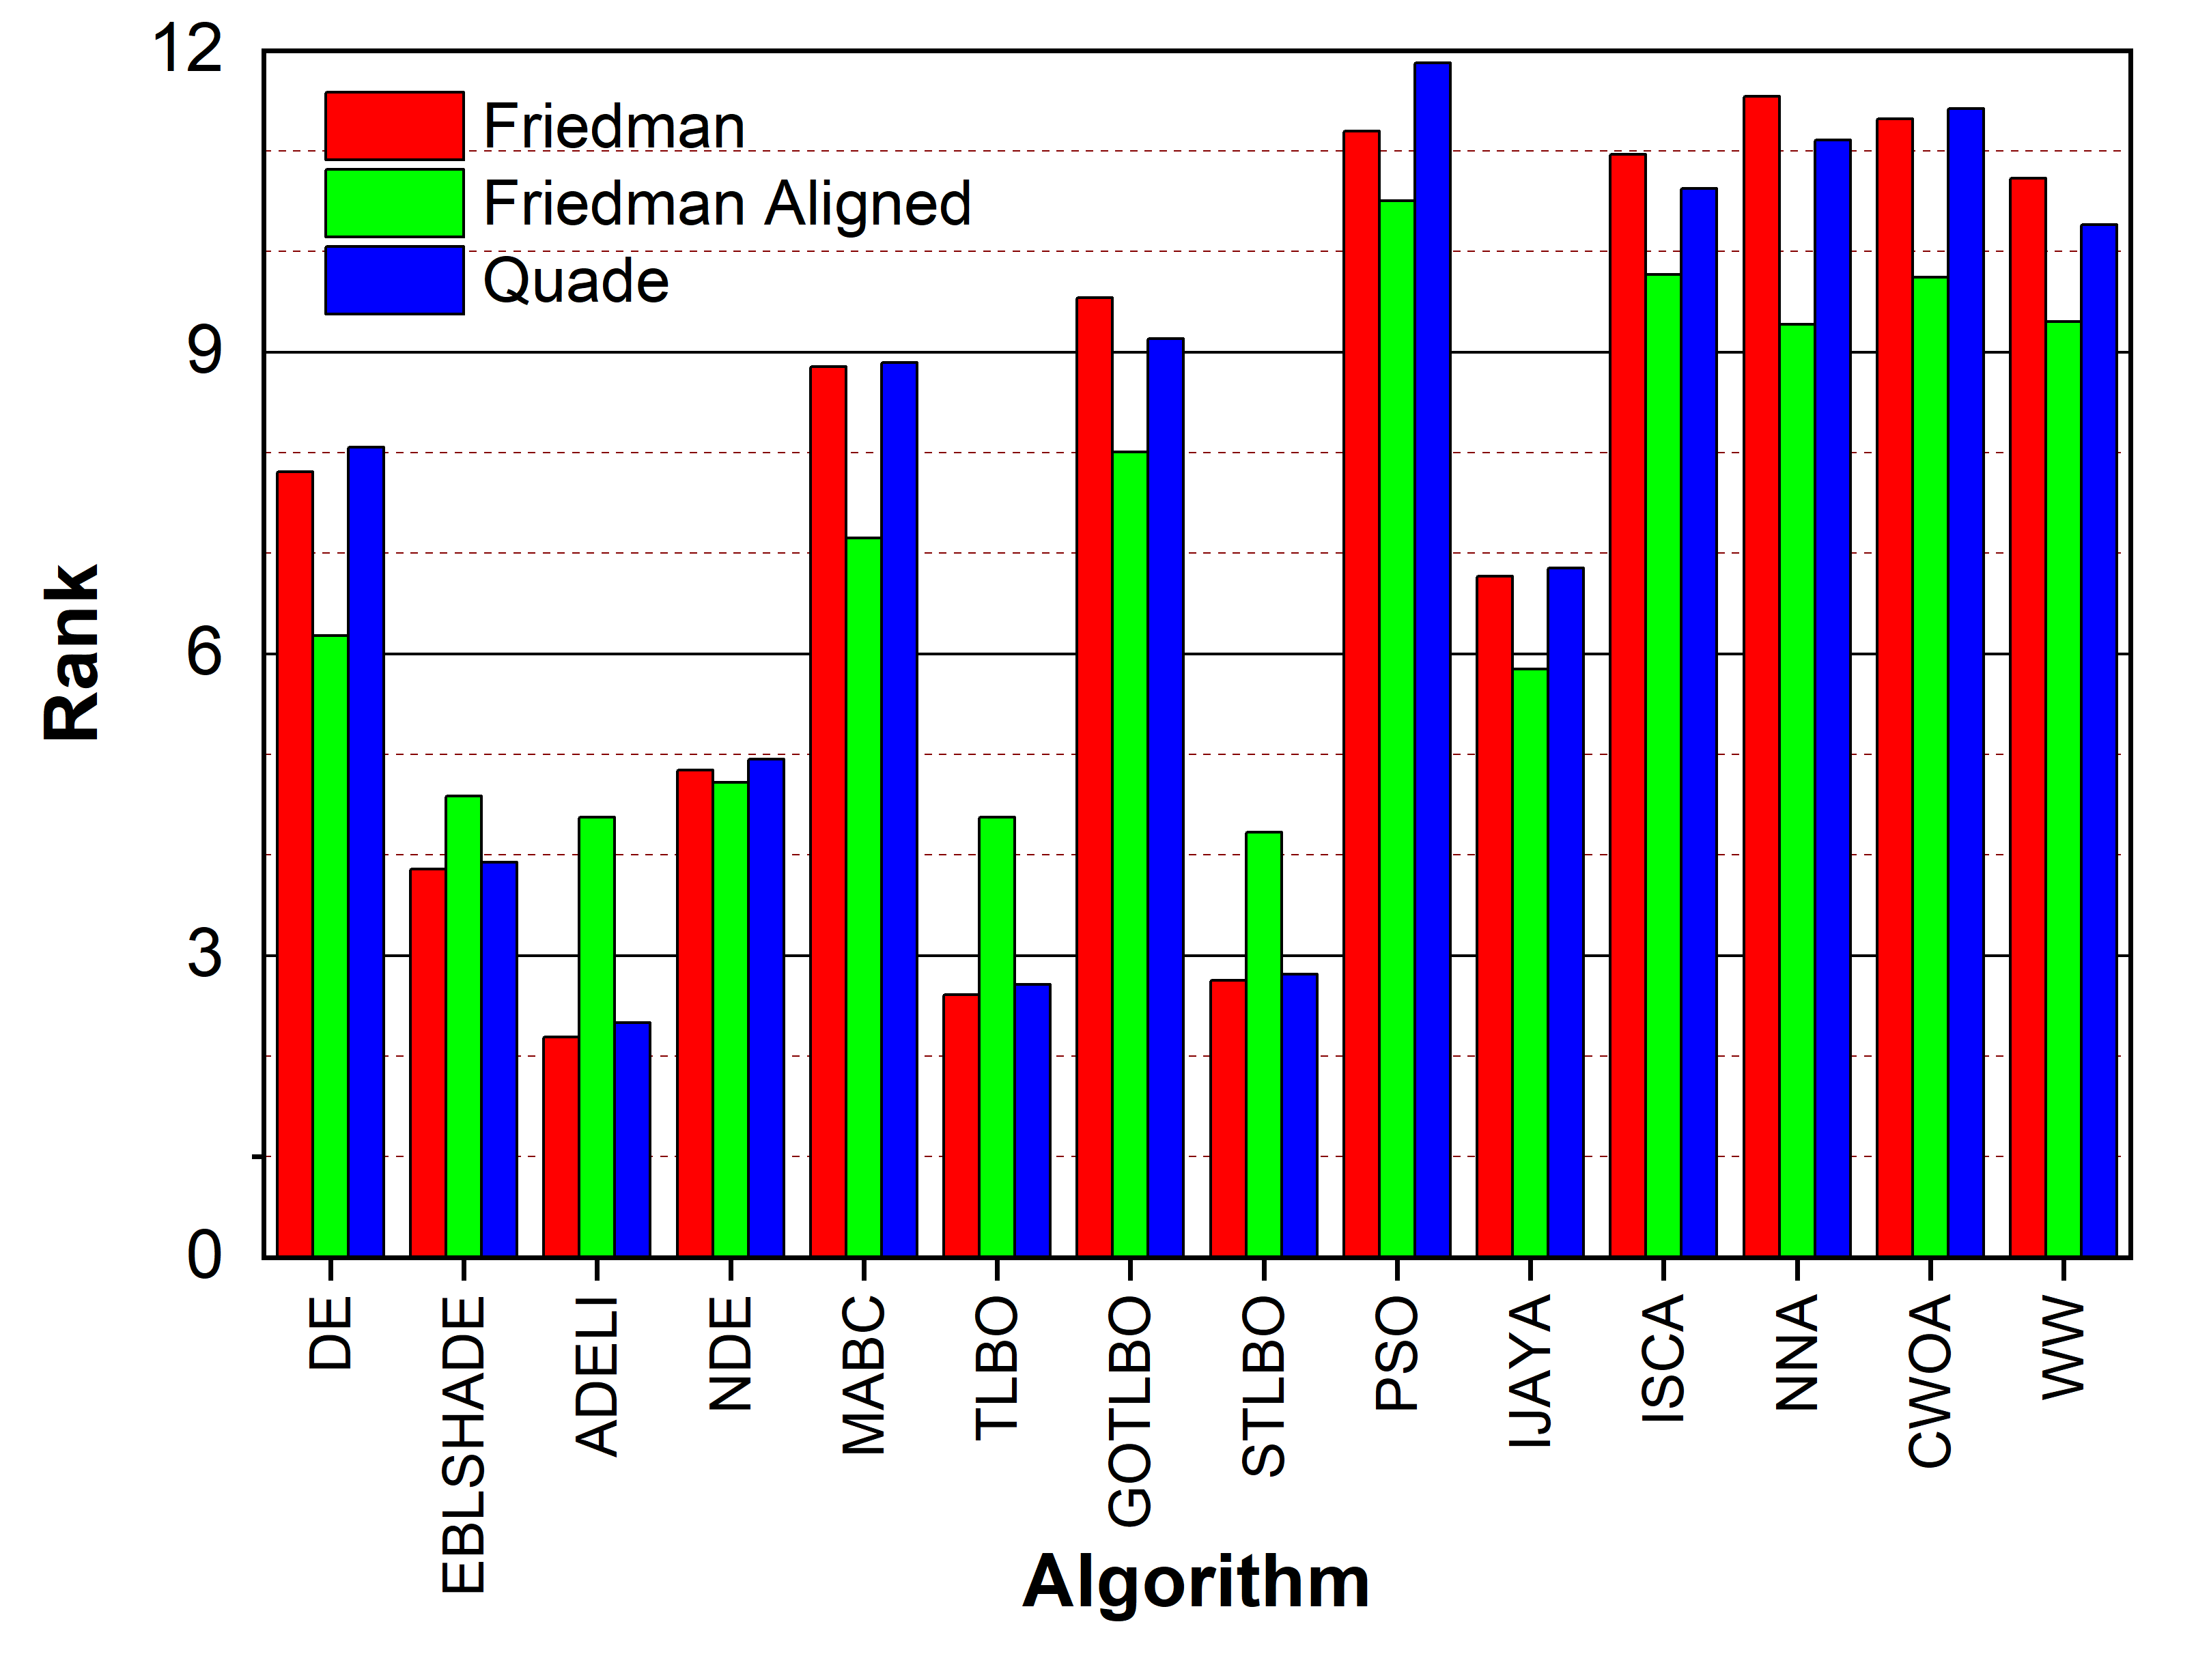
\includegraphics[width=0.5\columnwidth]{FigRankT}
	  \caption{Ranking of the algorithms according to Friedman, Friedman Aligned, and Quade tests in the IV-set case.}\label{figRankIVset}
\end{figure}



The presented data display several features similarly found in the single--\emph{IV} case.
For instance, the error in parameter estimation by mean values is higher than median value errors in most instances.
Exceptions arise at some temperatures, 
particularly when evaluating $I_{01}$ using IJAYA, 
$n_1$ using IJAYA and DE, 
$R_\mathrm{p1}$ using DE and MABC, 
and $R_s$ using DE and WW.
However, with high-precision algorithms, the deviation of MEDIAN from 
the true value does not exceed that of MEAN. 
Additionally, these algorithms exhibit small IQR values that do not exceed STD. 
Similar to the previous case, small RMSPE values do not always indicate high accuracy 
in determining the parameters of a solar cell.


At the same time, the number of algorithms exhibiting minimal errors has decreased.
Significant deviations from true values are observed for median values
of $I_{01}$, $n_{1}$, $R_\mathrm{p1}$, $n_2$, $R_s$, and $I_\mathrm{ph}$ evaluated by EBLSHADE at various temperatures,
as well as for median values of diode D1 characteristics and series resistor determined using TLBO at 260~K.
Thus, only ADELI and STLBO remain as algorithms without visible errors. 
Although this claim of infallibility applies only to median values, 
substantial errors are observed for mean values in several cases. 
Simultaneously, EBLSHADE, TLBO, IJAYA, and NDE constitute a group of algorithms with low RMSPE values 
but imperfect model parameter estimation.



In the \emph{IV}--set case, to assess the statistical performance of compared algorithms,
the run time and all $\mathrm{APE}_\mathrm{MEDIAN}$ and $\mathrm{RMSPE}_\mathrm{MEDIAN}$ values 
for each \emph{IV} curve were taken into account.
This approach mirrors the use of the Comp parameter in the previous subsection;
however, in this scenario, $N_\mathrm{pr}=81$ is employed:
\begin{equation*}
N_\mathrm{pr}= 10\,T_\mathrm{values}\times(8\,\mathrm{APE}_\mathrm{MEDIAN}+1\,\mathrm{RMSPE}_\mathrm{MEDIAN})+1\,t_\mathrm{run}\,.
\end{equation*}
Therefore, this approach is well--suited for nonparametric statistical analysis of $k=14$ meta--heuristic algorithms.
Certainly, at first glance, it would be interesting to consider incorporating an additional 80 values of the interquartile range into the dataset. 
This strategy could offer insight into the stability of algorithm performance as well.
However, it is known \cite{Derrac2011} that for multiple comparisons,
a value of$N_\mathrm{pr}\geq 8\cdot k=112$ could be too high, resulting in no significant comparisons.

%Будь-ласка, покращ англійську в наступних реченнях, які я буду пропонувати. Зокрема, треба буде виправити граматичні та стилістичні помилки
%якщо можна, окрім виправленого речення, наводь інформацію про зміни, які зроблені

Table~\ref{tblWilIVset} presents the statistical results generated by the Wilcoxon test. 
According to the table, ADELI outperforms all other algorithms with a significance level of $\alpha = 0.05$. 
STLBO and TLBO demonstrate improvements over DE, EBLSHADE, NDE, MABC, GOTLBO, PSO, IJAYA, ISCA, NNA, CWOA, and WW.

The counts of statistically significant cases $(+/=/-)$ are presented in the last row of Table~\ref{tblWilIVset}. 
It can be seen that PSO, ISCA, NNA, and CWOA did not outperform any of the algorithms,
whereas WW statistically significantly improved over NNA only.
Therefore, although these algorithms boast promising run times, 
they are not recommended for SC parameter estimation based on the opposed two-diode model.

The $p$--values required to test the null hypothesis, computed using the 
Friedman, Friedman Aligned, Quade tests, and the Iman-Davenport extension,
can be found in table~S2 of the supplementary materials. 
None of these values exceeds $2.3\cdot10^{-6}$, thus rejecting the hypothesis of equivalent medians in all tests.


Ranks achieved by the Friedman, Friedman Aligned, and Quade tests are shown in Fig..~\ref{figRankIVset} 
and table~S3 (supplementary material). 
According to the given results, ADELI has been placed first by the Friedman and Quade tests, 
while STLBO has ranked first by the Friedman Aligned test.

Ranks achieved by the Friedman, Friedman Aligned, and Quade tests are shown in Fig.~\ref{figRankIVset} and table~S3 in the supplementary material.
As per the given results, ADELI has been placed at first rank by Friedman and Quade tests,
and STLBO has ranked first by the Friedman Aligned test.
TLBO has been recorded as the second-best algorithm by all three tests. 
Furthermore, PSO was identified as the worst-performing algorithm by the tests' unanimous decision.




\begin{figure}[]
	\centering
%		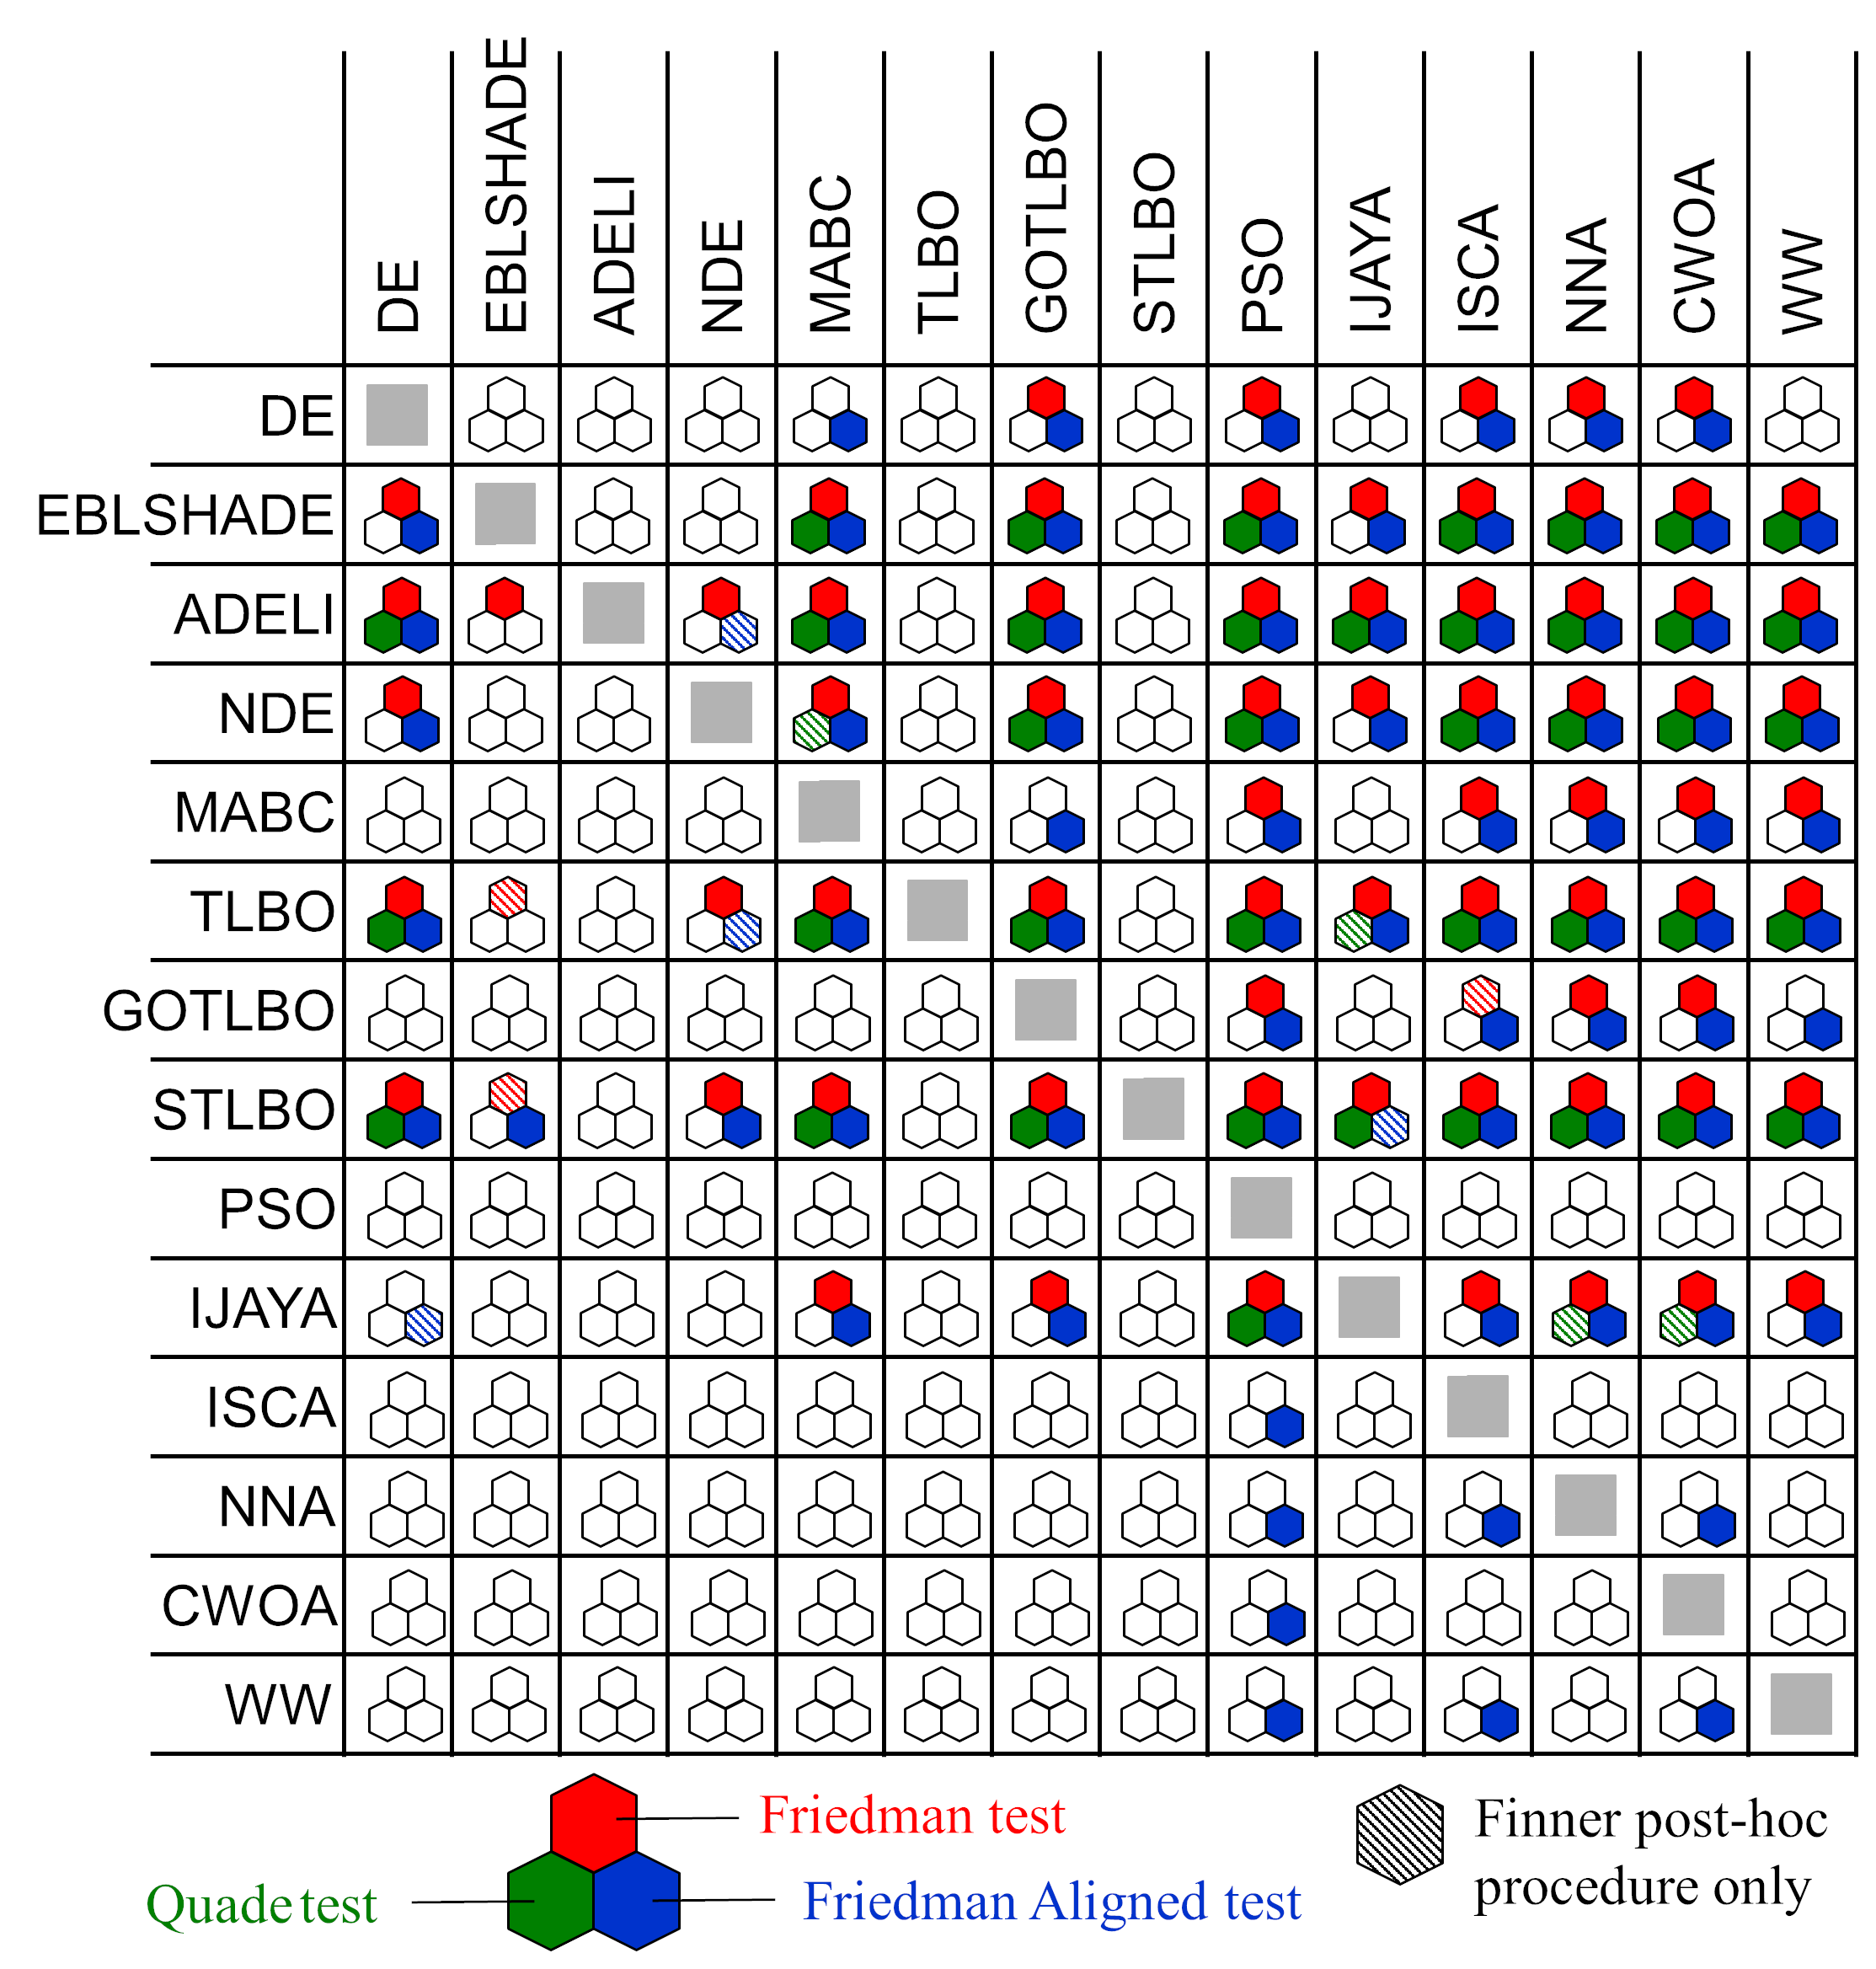
\includegraphics[width=1.0\columnwidth]{N1Tresult}
		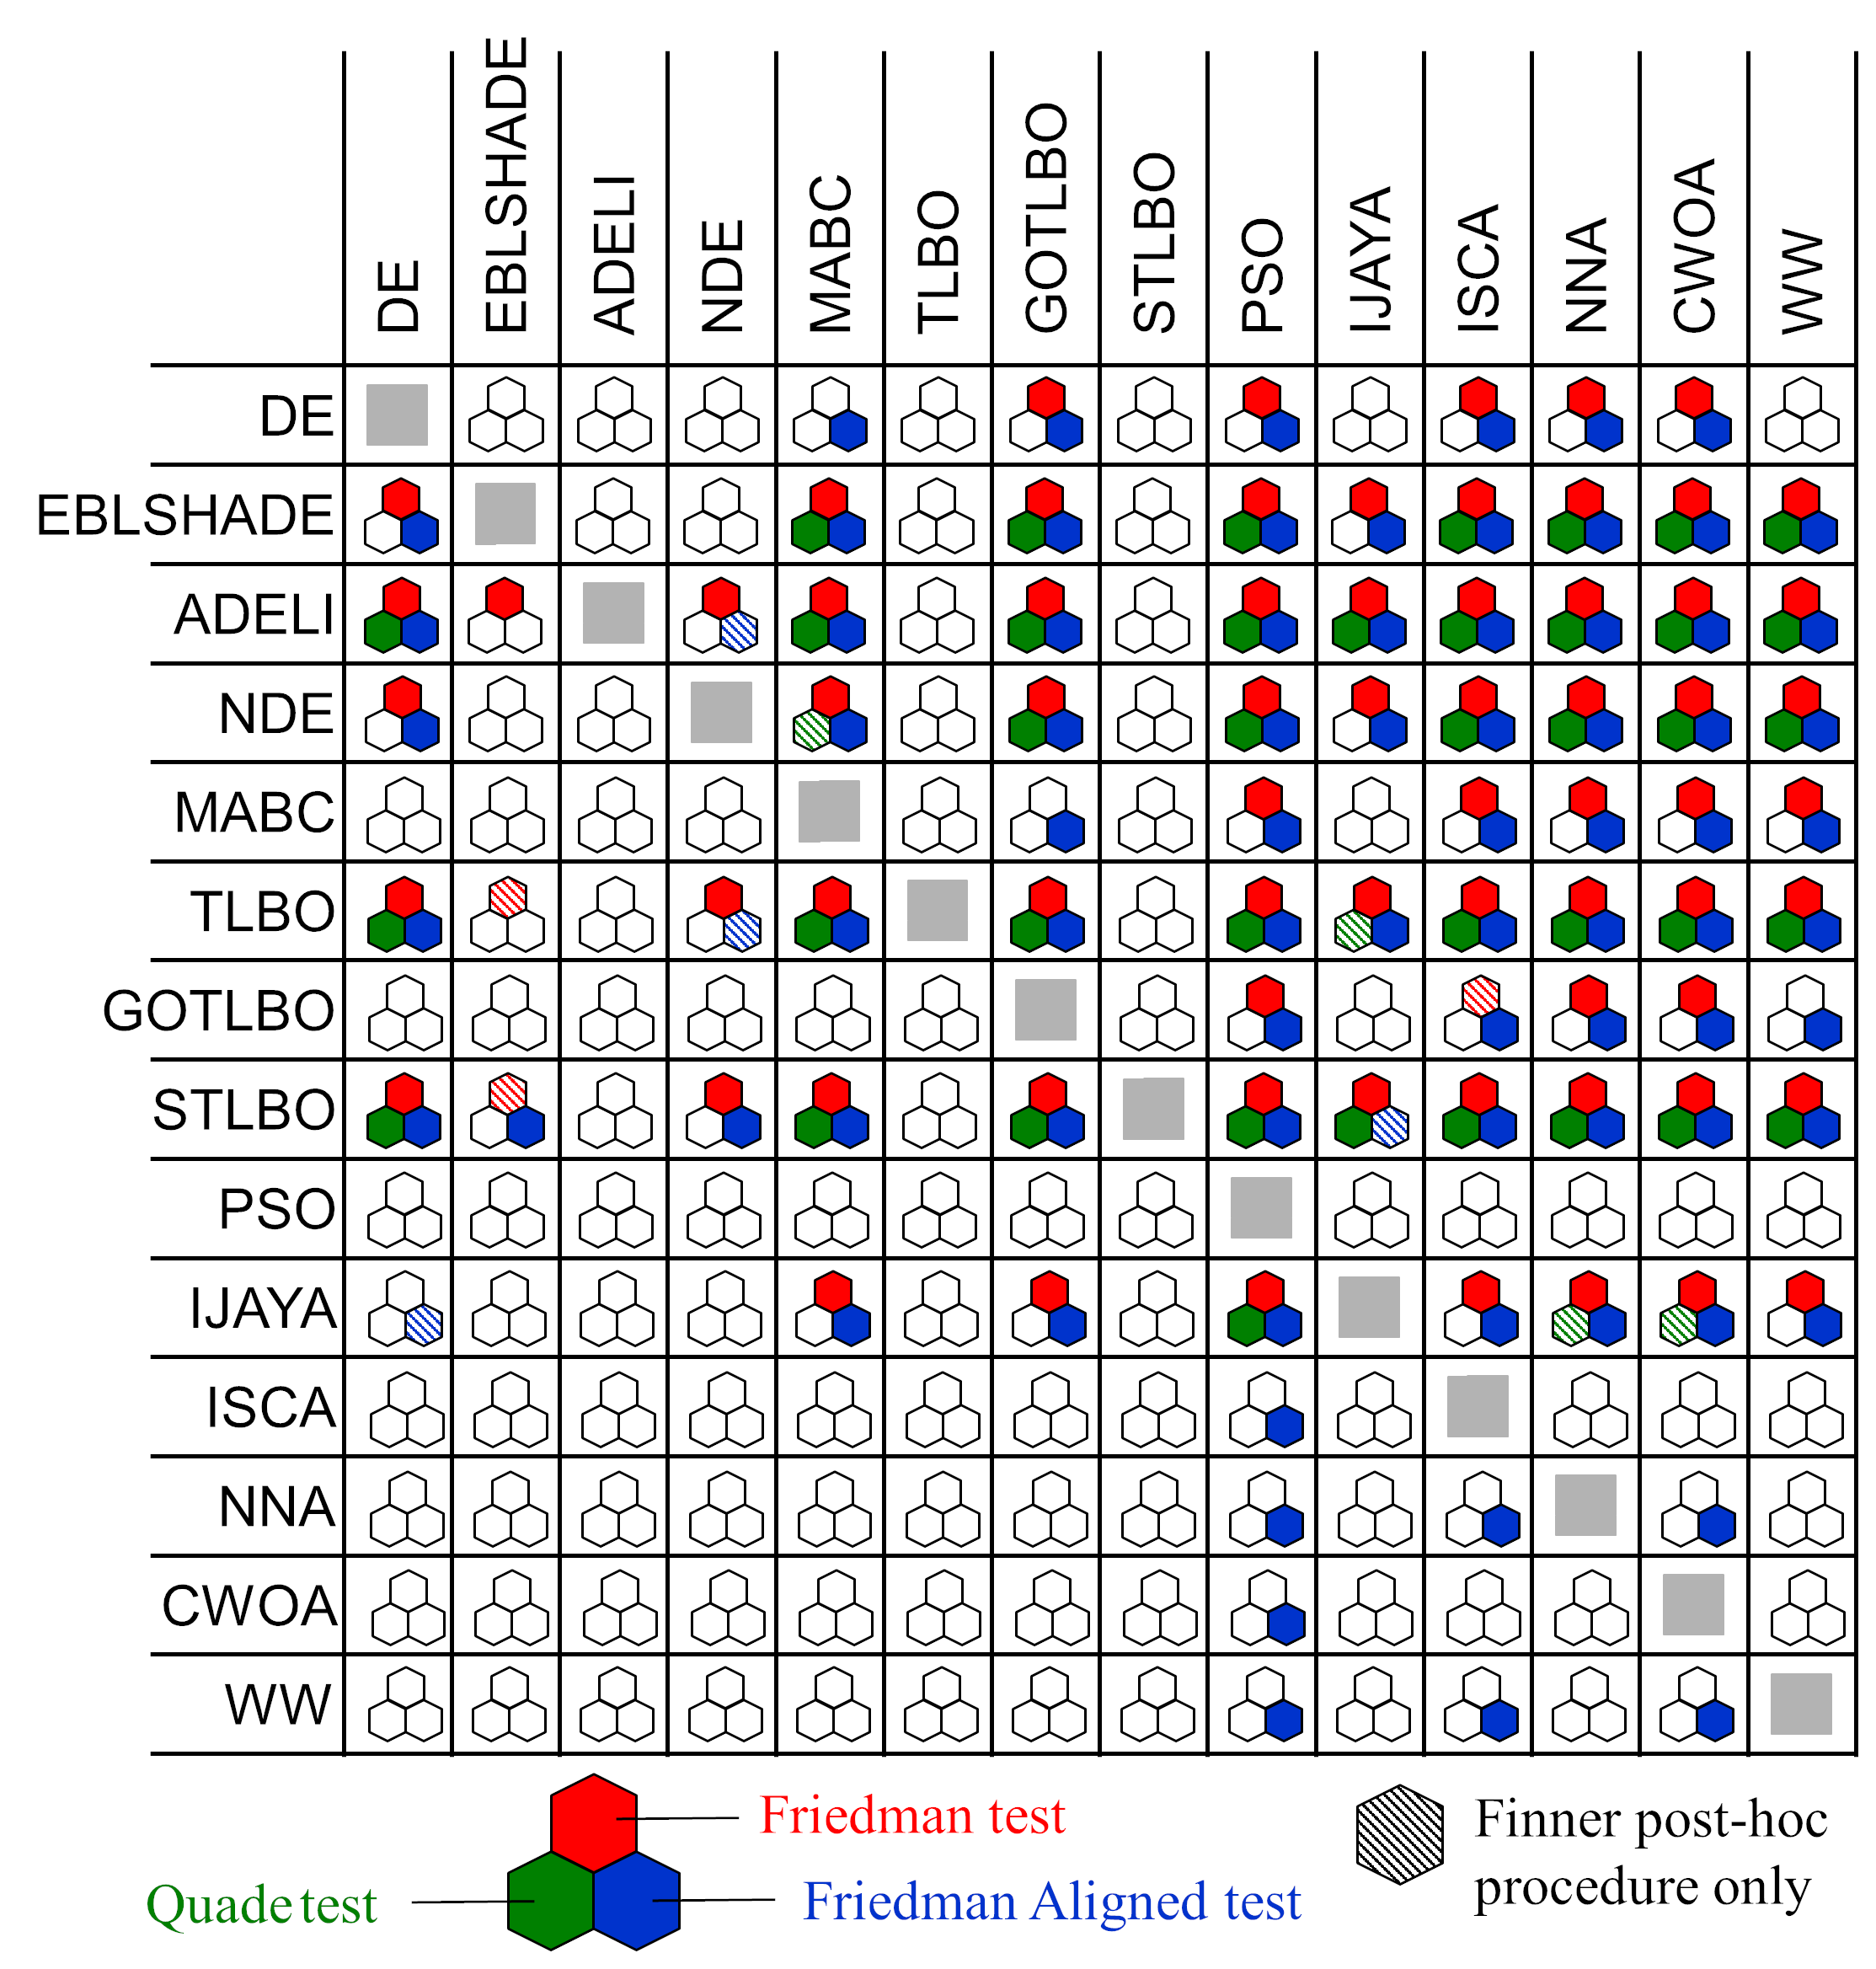
\includegraphics[width=0.5\columnwidth]{N1Tresult}
	  \caption{The results of algorithm $1\times N$ comparisons by Friedman, Friedman Aligned, and Quade tests in the IV-set case.
               The colored hexagon indicates that the adjusted $p$-value,
               which tests the hypothesis that an algorithm in a row outperforms the algorithm in a column,
               is not greater than $p_{cr}=0.1$.
               The solid fill signifies that every post-hoc procedure resulted in $p<p_{cr}$;
               the dashed fill indicates that the Finner post-hoc procedure was the only method that produced this result.
               The correspondence between the color and position of the hexagon to a test
               is shown in a legend at the bottom of the figure.
               }\label{figN1RezIVset}
\end{figure}


\begin{figure}[]
	\centering
%		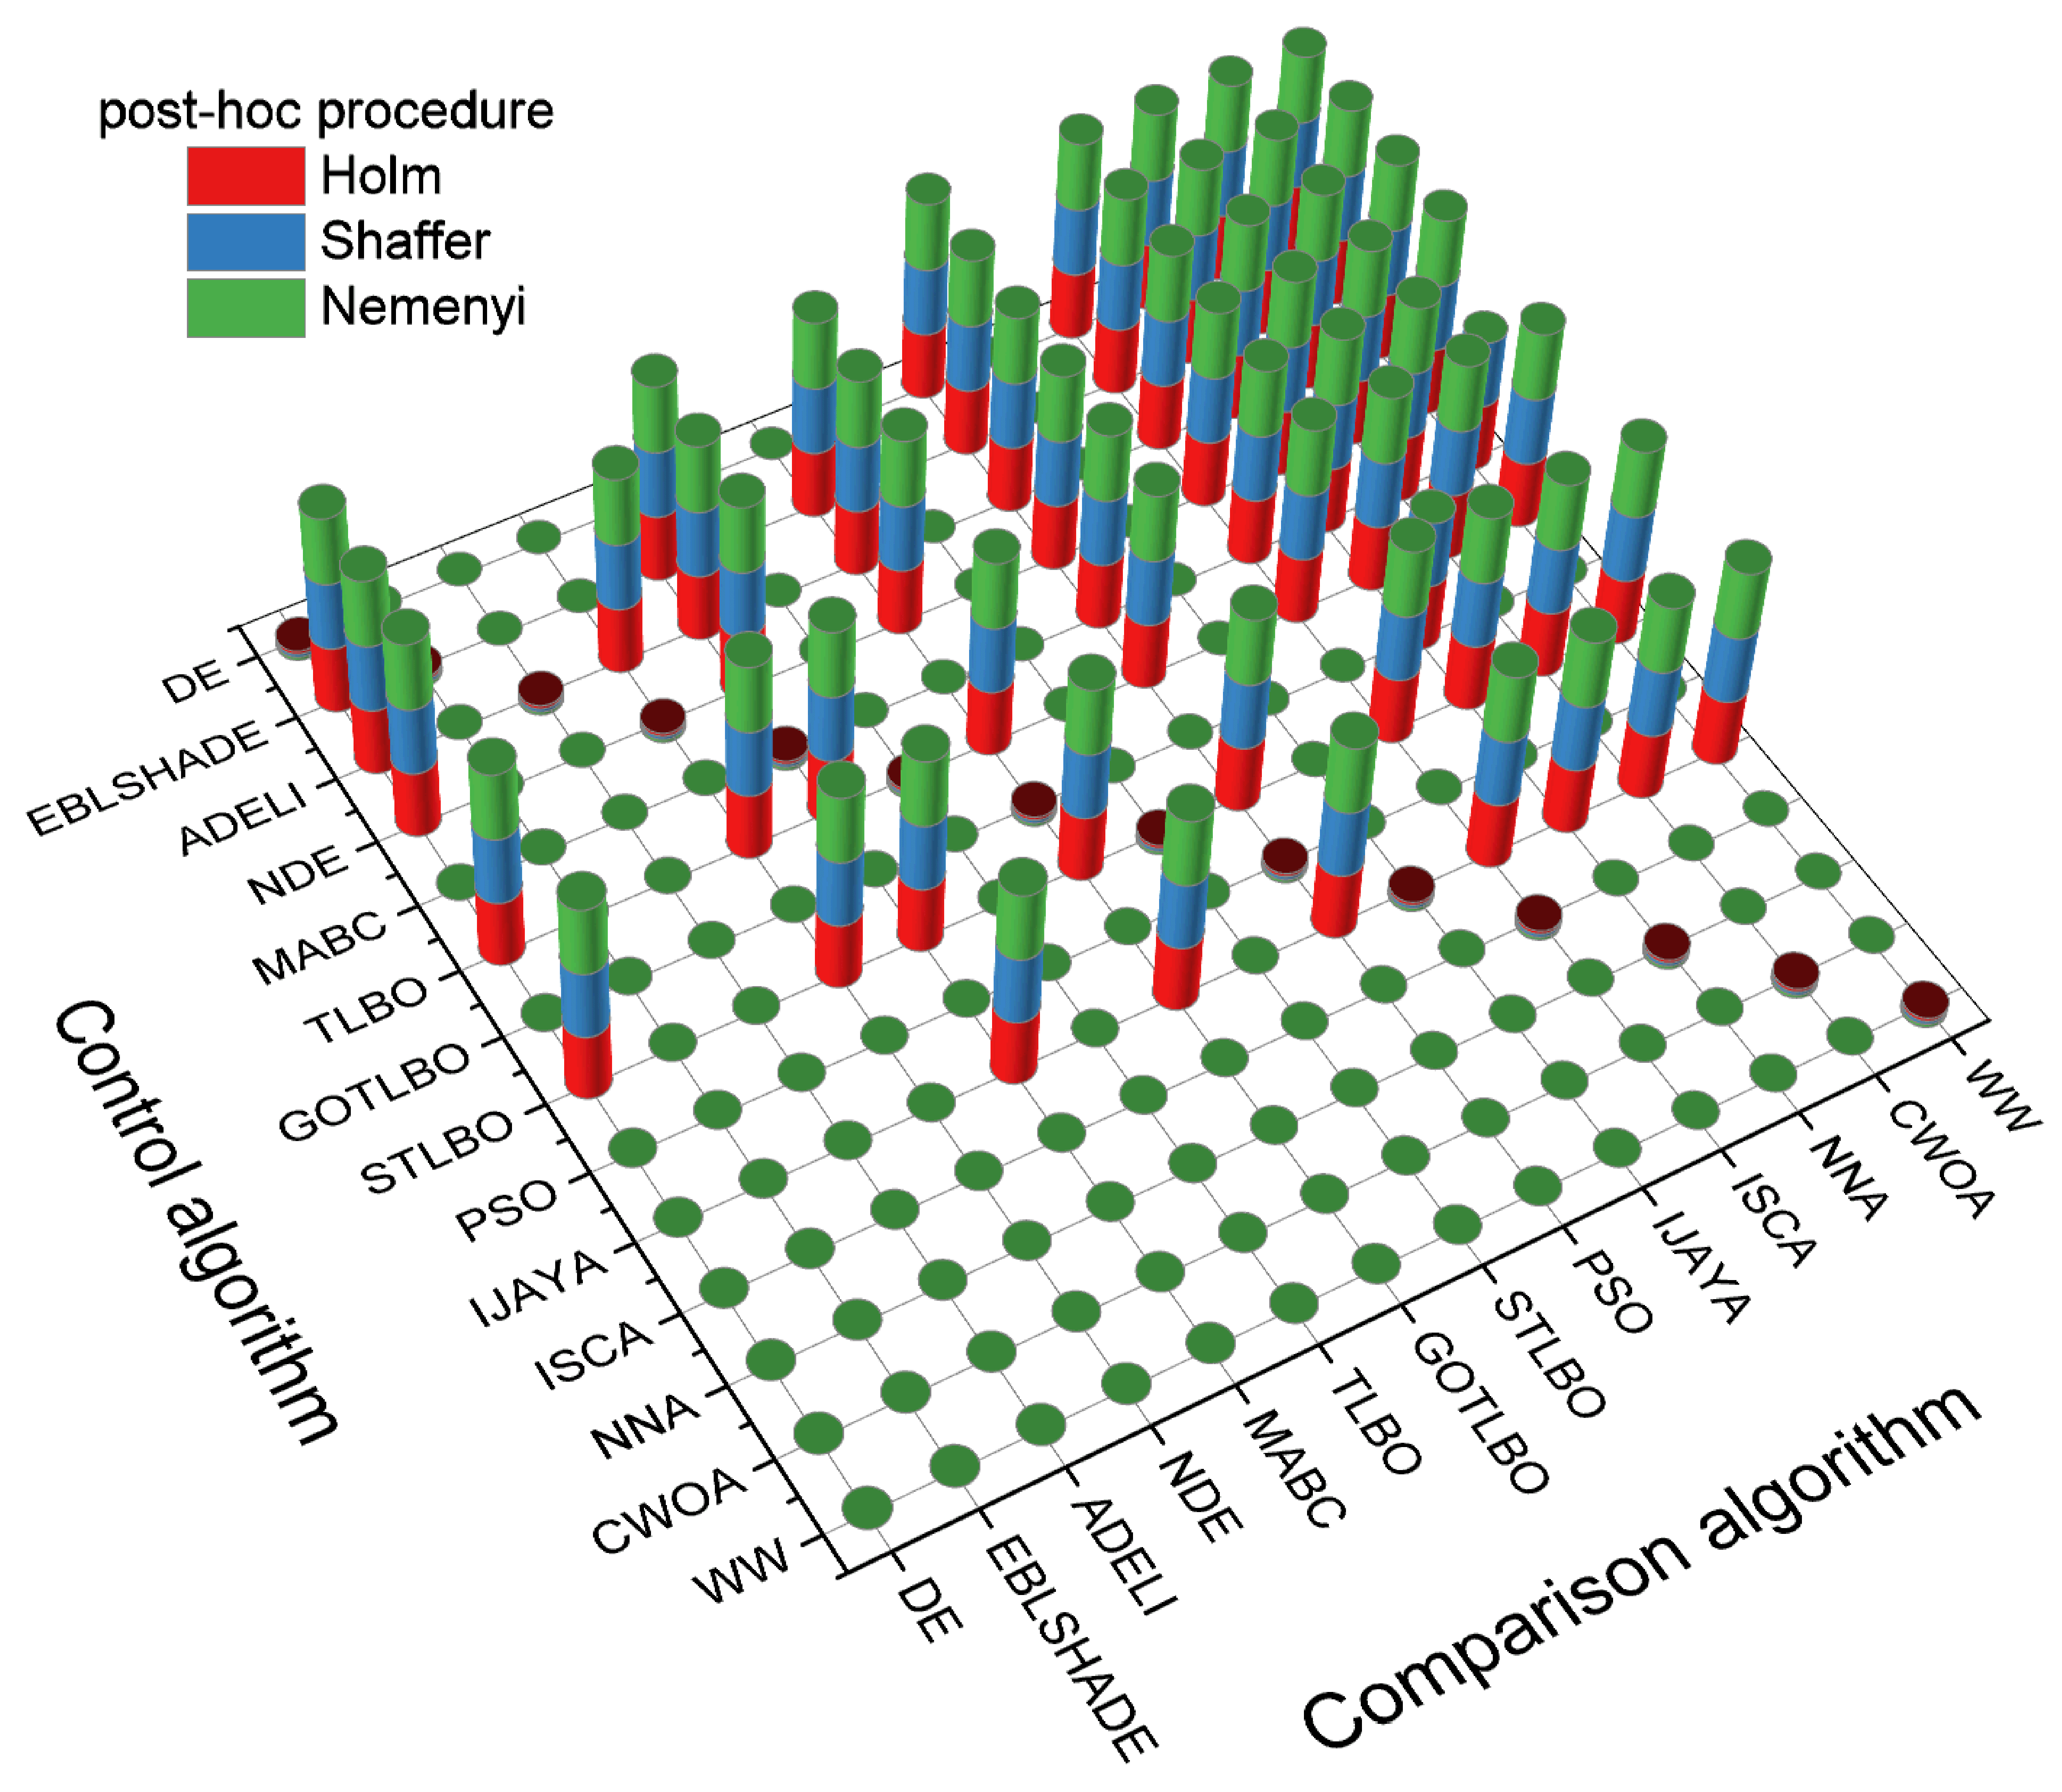
\includegraphics[width=1.0\columnwidth]{NNresult}
		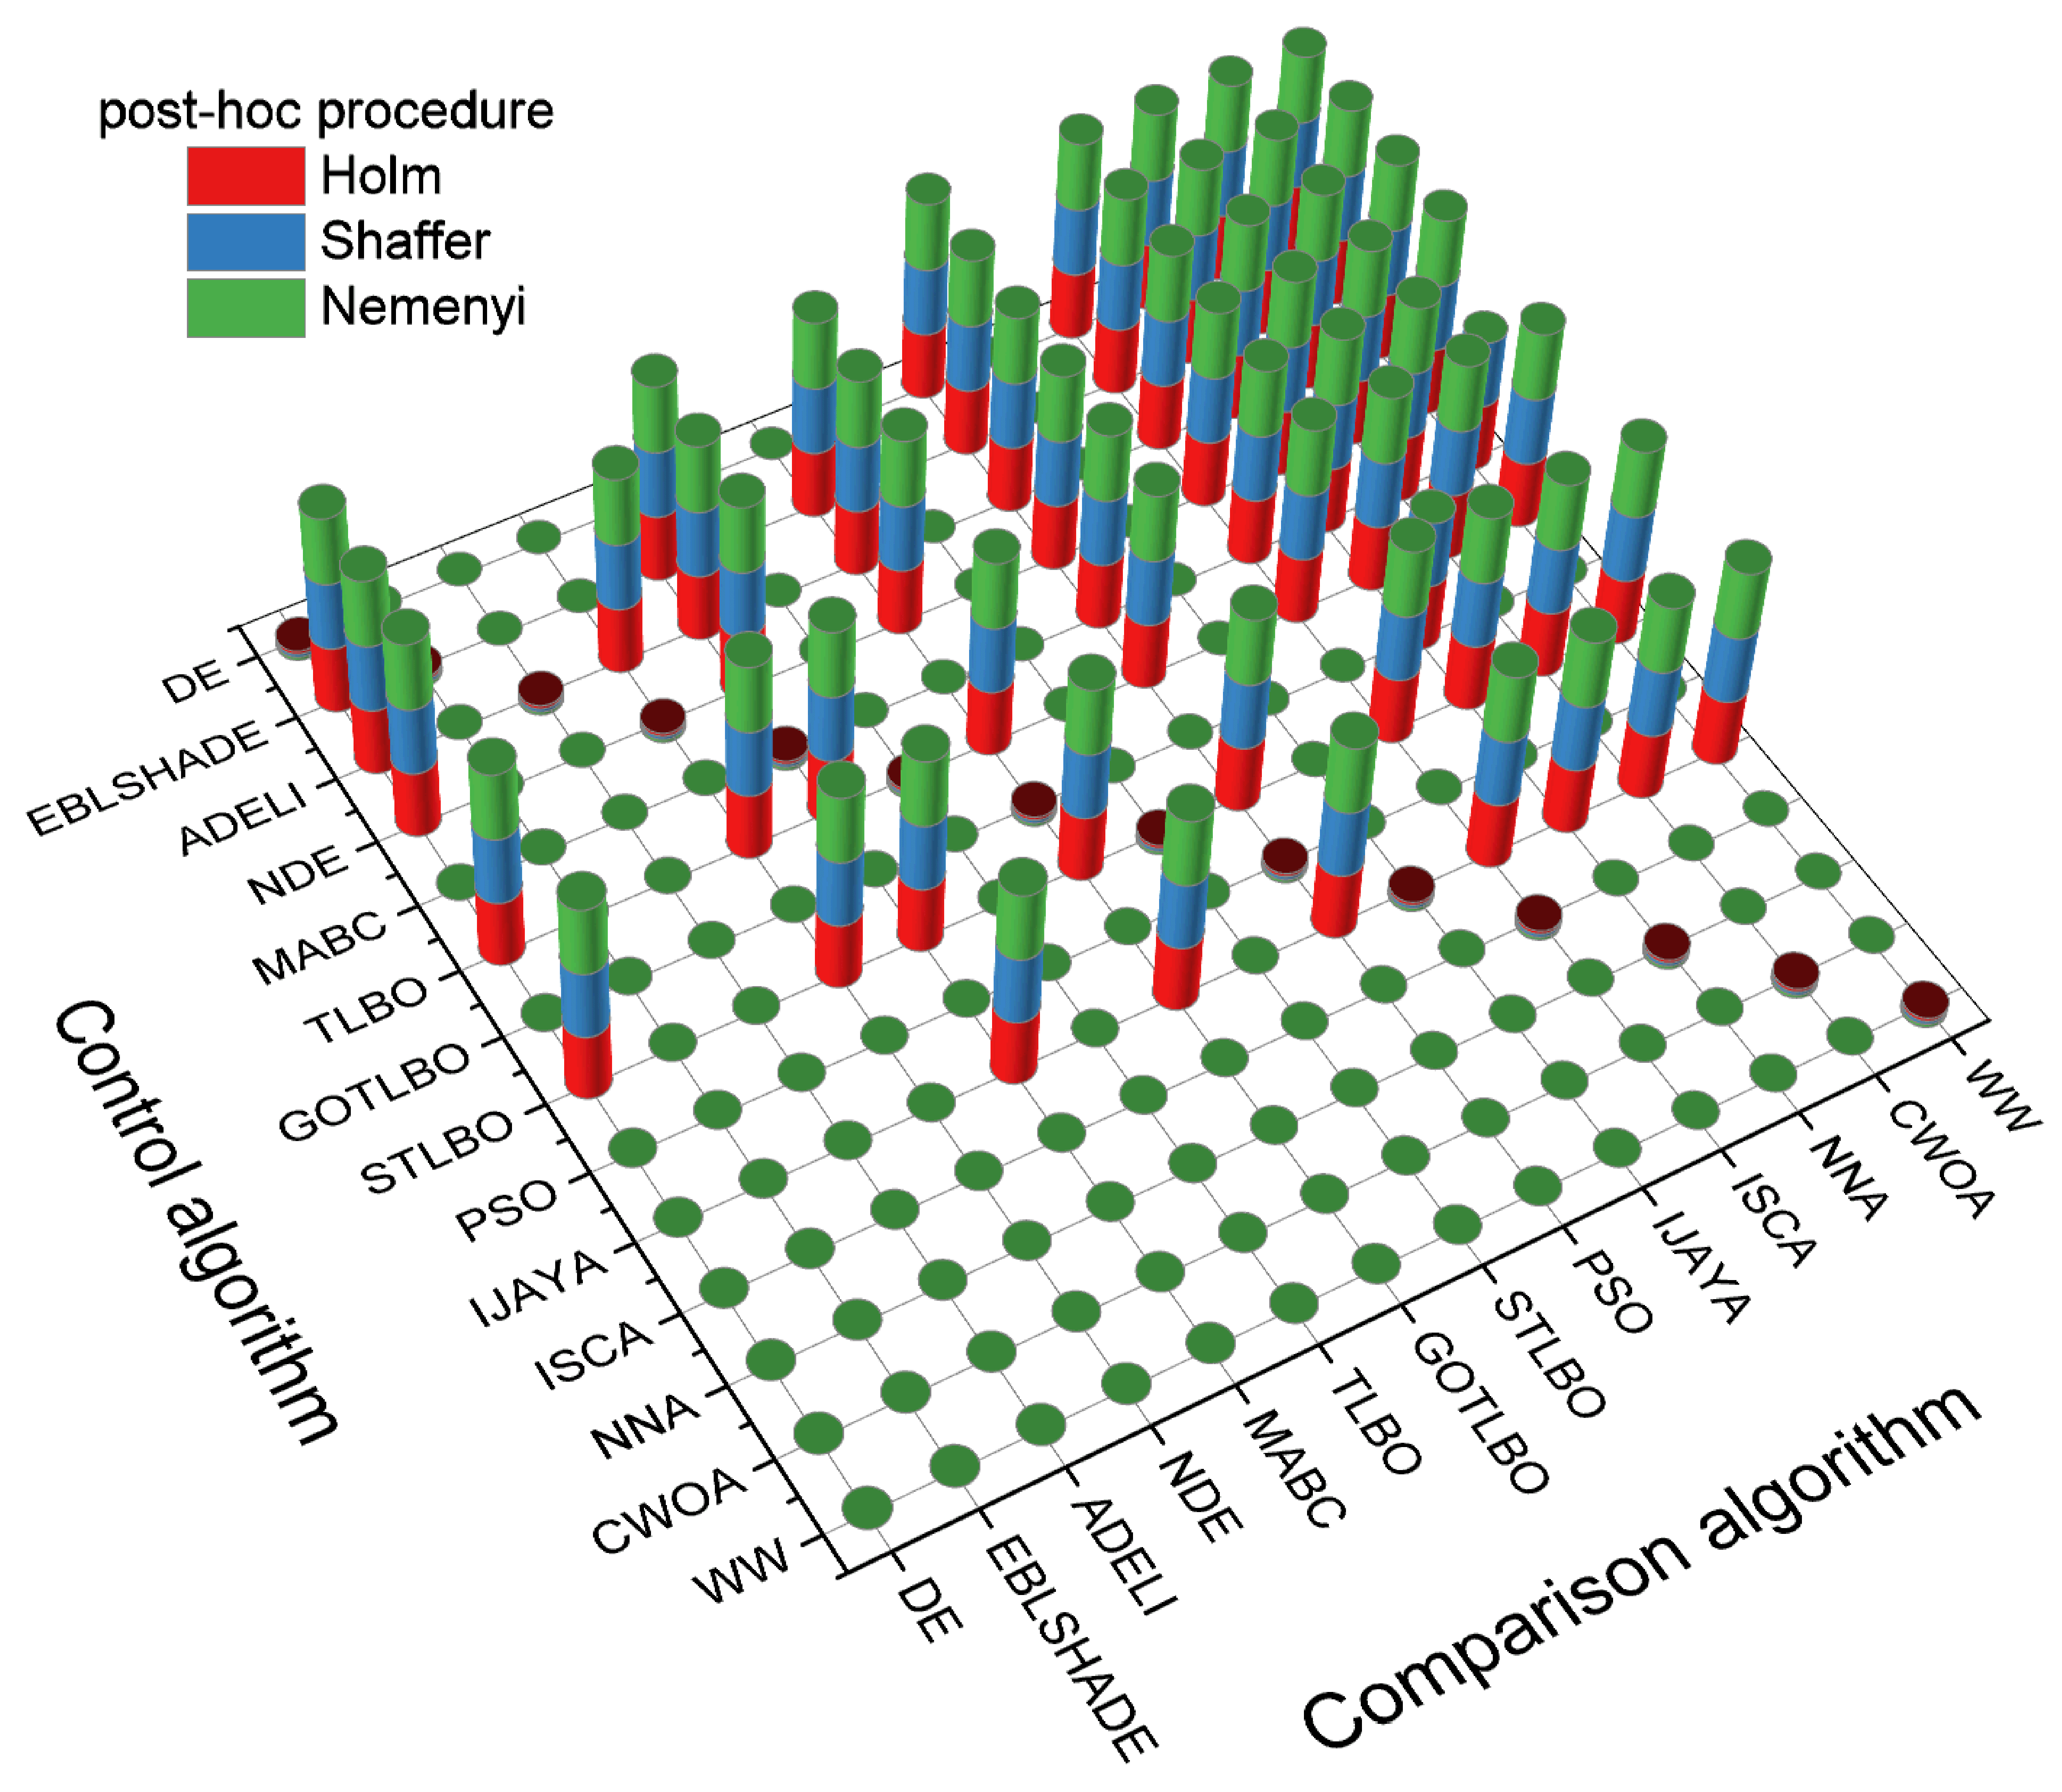
\includegraphics[width=0.5\columnwidth]{NNresult}
	  \caption{The results of multiple comparisons among all algorithms in the IV-set case.
               The colored cylinder indicates that the adjusted p-value,
               which tests the control algorithm outperforms the comparison algorithm,
               is not greater than $p_{cr}=0.1$.
               The correspondence between the color of the cylinder to a post-hoc procedure is shown in the figure's legend.
               }\label{figNNRezIVset}
\end{figure}

\begin{table}[<options>]
\caption{The total count of wins and losses for each algorithm in $1\times N$ and $N\times N$ multiple comparisons using the
all tests and post-hoc procedures in the IV-set case.
The criterion for victory was a adjusted $p$-value less than 0.1.
The best results are bolded.
}\label{tblAllWins}
\begin{tabular*}{\tblwidth}{@{}LCC@{}}
\toprule
\multirow{2}{*}{Algorithm}& \multicolumn{2}{C}{Wins / Loses} \\
  & $1\times N$ comparisons& $N\times N$ comparisons\\ % Table header row
\midrule
DE & 44/53 & 15/15\\
EBLSHADE & 100/6 & 24/\textbf{0} \\
ADELI & 117/\textbf{0} & \textbf{27}/\textbf{0}\\
NDE & 97/18 & 24/9\\
MABC &  44/69 & 14/18\\
TLBO & 111/\textbf{0} & \textbf{27}/\textbf{0}\\
GOTLBO & 25/80 & 2/18\\
STLBO & \textbf{118}/\textbf{0} & \textbf{27}/\textbf{0}\\
PSO & 0/112 & 0/24\\
IJAYA &  63/46 & 21/\textbf{0}\\
ISCA & 4/97 & 0/24\\
NNA & 12/93 & 0/26\\
CWOA & 4/101 & 0/24\\
WW & 12/80 & 0/23\\
\bottomrule
\end{tabular*}
\end{table}




The $p$-values, obtained for $1\times N$ multiple comparisons are shown in tables~S155-168 in the supplementary material.
There are results of applying  Finner, Holm, Hochberg, and Holland procedures,
as a post-hoc method after Friedman, Friedman Aligned, and Quade tests.
The reader is referred to supplementary material (table~S169) for $p$-values of
applying  Shaffer, Nemenyi, and Holm post-hoc procedures after the Friedman test in the
case of $N\times N$ multiple comparisons.
The results, which determine whether one algorithm yielded a statistically better estimation of parameters
than the other (with a $p$-value $\leq p_{cr}=0.1$), are summarized in Fig.~\ref{figN1RezIVset} and \ref{figNNRezIVset}
for $1\times N$ and $N\times N$ comparisons, respectively.
The counts of statistically  significant cases are presented in the Table~\ref{tblAllWins}.

As can be seen,
ADELI, TLBO, and STLBO were never outperformed by any of the algorithms,
both in the case of $1\times N$ and $N\times N$ multiple comparisons.
By the way, for $N\times N$ comparisons, the same property is observed with EBLSHADE and IJAYA.
Overall, the parameter estimation results obtained from the set of IV curves
using ADELI, TLBO, and STLBO algorithms for $N\times N$ comparisons in the opposed two-diode model are practically indistinguishable
(when it comes to precise $p$-values, only minor differences can be observed).
In $1\times N$ comparisons, TLBO demonstrates lower performance compared to ADELI and STLBO,
in terms of efficiency when compared to the EBLSHADE algorithm.
Specifically, the improvement of TLBO over EBLSHADE is proved only by the Finner procedure applied in the Friedman test.
Based on $1\times N$ comparisons, it is observed as well that there are slight differences between ADELI and STLBO,
primarily when compared to the non-worst algorithms.
For instance, the Quade test confirms the improvement of ADELI over EBLSHADE for every post-hoc procedure,
however, the Friedman and Friedman Aligned tests did not show statistically significant differences between these algorithms.
Meanwhile, the Friedman Aligned and Quade tests find a difference between STLBO and EBLSHADE
for every post-hoc procedure and Finner procedure only, respectively.
Regarding comparison with NDE, the Friedman Aligned test demonstrated that STLBO is better according to all post-hoc procedures.
In contrast, for ADELI, this outperforming was only observed using the Finner method.
In the case of IJAYA,
the results of the Friedman Aligned test show a reversal:
only the Finner procedure indicates an improvement for STLBO,
whereas ADELI outperforms all post-hoc methods utilized.

In deciding the optimal algorithm for parameter estimation of solar cell parameters
from the IV curve using the opposed two-diode model,
the practical choices boil down to EBLSHADE, ADELI, TLBO, and STLBO.
However, TLBO exhibited lower performance when applied in the single-IV case.
The parameter estimation error when using EBLSHADE was not always minimal in the IV-set case.
Despite the minimal advantage in terms of win counts in $1\times N$ comparisons
(see Table~\ref{tblAllWins}),
we hesitate to declare STLBO as the best.
In our opinion, STLBO and ADELI both hold the top position in the competition conducted in this study.



Over the last few decades, researchers have strived to enhance the performance of metaheuristic algorithms using various concepts, including \cite{Kepler}:
hybridization between two or more metaheuristics, quantum computing concept, opposition-based theory, chaotic maps,  L\'{e}vy-Flight strategy.
Our research has revealed that the most promising approaches to solving
the parameter estimation problem for S-shaped \emph{IV} curves involve the use of enhanced mutation strategies.
Specifically, this entails employing chaotic maps to tune mutation coefficients and utilizing the elite strategy (STLBO).
Furthermore, highly productive results were achieved through the application of nonlinear (polynomial) approximation of potential solutions (ADELI).




\section{Conclusion}\label{SecConsl}

In this paper, the possibility of using meta--heuristic algorithms
to solve the parameter estimation problems of photovoltaic cells
with S--shaped current--voltage characteristics has been explored.
The parameter estimation has been performed within the framework of the opposed two-diode model.
A total of 14 meta--heuristic algorithms from various classes were implemented
to extract the solar cell parameters from synthetic IV curves, which were generated with a range of parameter values.
The obtained results have been compared using nonparametric statistical procedures,
including pairwise comparisons, $1\times N$ multiple comparisons, and $N\times N$ multiple comparisons.

Research has demonstrated that utilizing a squared error-based fitness function offers clear advantages in tackling a provided problem.
The overall performance results of various algorithms generally fit the No Free Lunch theory.
%‘‘No-Free-Lunch’’ theorem.
GOTLBO, PSO, ISCA, NNA, CWOA, and WW are completely unsuitable for parameter estimation according to the opposed two-diode model.
The results of DE, NDE, MABC, and IJAYA are not as poor as those in the previous group;
however, in general, it is still not recommended to use these algorithms for solving parameter identification problems.
Generally, the EBLSHADE and TLBO are effective in accurately determining parameter values in most cases.
However, investigation has shown that these algorithms may make mistakes under certain conditions.
Therefore, EBLSHADE and TLBO applications in the case of solar cells with S-shaped IV curves should be approached with caution.
Finally, results have illustrated that STLBO and ADELI have superior performance in terms of accuracy and reliability
when compared with other used algorithms.
In particular, these two algorithms successfully solve the task of accurately determining parameters
from similar IV curves corresponding to photovoltaic cells with distinct characteristics.

It is important to note that in this study,
the parameters were obtained from idealized IV curves,
where the voltage-current relationships were precisely defined by Eq.~(\ref{eqIV_g}).
In a real experiment, there is a potential for errors in the measurement of both current and voltage.
Hence,  it would be worthwhile to explore the efficacy of various meta--heuristic algorithms
in determining parameters from IV data corrupted by noise in future research.

This work of testing and comparative analysis of
different meta--heuristic algorithms for the estimation
of solar cell parameters should be useful for further research and development on photovoltaic systems.


\section*{Supplementary data}
Supplementary data to this article can be found online at
\url{http://surl.li/phuem}

%\section*{CRediT}
%O.~Olikh: Conceptualization, Methodology, Software, Formal analysis, Writing - Original Draft, Writing - Review \& Editing.
%L.~Olikh: Validation, Data Curation, Writing - Original Draft, Visualization.

%https://www.mediafire.com/file/935ys71ak88jwp5/SupplementaryMaterial.pdf/file
%https://www.mediafire.com/file/io7oz2rh59s7k6b/SupplementaryMaterial.pdf/file
%https://www.mediafire.com/file/29s6gxrz4l19u6k/SupplementaryMaterial.pdf/file
\section*{Data availability}
Data will be made available on request.


\bibliographystyle{model1-num-names}
\bibliography{olikh_Methods}


\end{document}




